\documentclass[
  11pt,             % 10pt | 11pt | 12pt
  french,           % french | english
  greyCover,        %
  fancyChapter,     %
  fancyPart,        %
  %squeezeCommittee %
  %showframe        %
]{these-LUNAM_mod}

%\usepackage{etex}                            % solve compatibility issues
\usepackage[utf8]{inputenc}                   %
\usepackage[T1]{fontenc}                      %
\usepackage{textcomp}                         % °, <<, >>, etc.
\usepackage{times}                            %
\usepackage{natbib}                           %
\usepackage{xifthen}                          %
\usepackage{relsize}                          % \mathlarger
\usepackage{multirow}                         %
\usepackage{booktabs}                         % \addlinespace, \toprule, etc.
\usepackage{subfigure}                        %
\usepackage{tikz}                             %
\usepackage{pgfplots}                         %
\usepackage{makeidx}                          %
\usepackage{amsthm}                           % theorem definition and styling
\usepackage{epigraph}                         % chapter heading quote
\usepackage[inline]{enumitem}                 %
\usepackage{ragged2e}                         % \justifying
\usepackage{rotating}                         % \sideways in table
\usepackage{lipsum}                           %
\usepackage{mathabx}                          % $\drsh$
\usepackage[ruled,linesnumbered]{algorithm2e} %
\usepackage{listings}                         %

\usetikzlibrary{positioning, topaths, shapes, arrows, patterns}

\setlength\epigraphwidth{10cm}
\setlength\epigraphrule{0cm}

\RequirePackage[bookmarks,
                colorlinks,
                urlcolor=black,
                citecolor=black,
                linkcolor=black,
                hyperfigures,
                pagebackref,
                pdfcreator=LaTeX,
                breaklinks=true,
                pdfpagelayout=SinglePage,
                bookmarksopen=true,
                bookmarksopenlevel=2]{hyperref}

\geometry{inner=2.5cm, outer=2.5cm, top=2.5cm, bottom=2cm}
\geometry{inner=3.5cm, outer=3.5cm, top=4cm, bottom=3.5cm} % CUSTOM
%\geometry{inner=1.5cm, outer=1.5cm, top=2cm, bottom=2cm}

\setlist[enumerate]{itemsep=0mm}  % minimum spacing between items (it is not
\setlist[itemize]{itemsep=0mm}    % same as \setlist[...]{noitemsep}
\renewcommand{\labelitemi}{--}
\renewcommand{\labelitemii}{-}
\renewcommand{\labelitemiii}{-}
\renewcommand{\labelitemiv}{-}

%-------------------------------------------------------------------------------
\newcommand\setlstxml{
  \footnotesize
  \lstset{language=XML}
  \lstset{morekeywords={
    notice, titre, resume, encoding, TEI, xmlns, xmlns:tei, teiHeader, fileDesc,
    sourceDesc, biblStruct, type, analytic, title, author, persName, ana,
    forename, surname, profileDesc, abstract, p, martif, martifHeader, text,
    body, termEntry, langSet, tig, term, xml:id, stdf, soHeader, annotations,
    annotationGrp, target, span, from, num, link, note
  }}
  \lstset{literate={'}{{'}}1 {é}{{\'e}}1 {è}{{\`e}}1 {ê}{{\^e}}1 {à}{{\`a}}1 {ô}{{\^o}}1}
  \lstset{frame=single}
  \lstset{stringstyle=\color{red}}
  \lstset{keywordstyle=\color{blue}}
}

%-------------------------------------------------------------------------------

\newcommand\chaptercite[2]{\epigraph{\justifying{\Large``}\textit{#1}{\Large''}}{--- #2}}
\newcommand\smallchaptercite[2]{\epigraph{\hfill{}{\Large``}\textit{#1}{\Large''}}{--- #2}}

\newcommand\ditto{$_{^\textnormal{\normalsize\textquotedbl}}$}

\renewcommand\cite[2][]{\ifthenelse{\equal{#1}{}}{\citep{#2}}{\citep[#1]{#2}}}
\newcommand\newcite[2][]{\ifthenelse{\equal{#1}{}}{\citet{#2}}{\citet[#1]{#2}}}

\newcommand\TODO[1]{\textcolor[rgb]{1, 0, 0}{[TODO #1]}}
\newcommand\REMARK[1]{\textcolor[rgb]{0, 1, 0}{[#1]}}
\newcommand\ANNOTATE[2]{\textcolor{blue}{[#1 \textbf{$\rightarrow$ #2}]}}
\newcommand\FILL[1]{\textcolor{red}{\lipsum[#1]}}

\theoremstyle{remark}
\newtheorem{example}{Exemple}

\makeindex

%%%%%%%%%%%%%%%%%%%%%%%%%%%%%%%%%%%%%%%%%%%%%%%%%%%%%%%%%%%%%%%%%%%%%%%%%%%%%%%%

\titre{Indexation automatique par termes-clés\\en domaines de spécialités}
%\soustitre{}

\title{Automatic Domain-Specific Keyphrase Annotation}
%\subtitle{}

\author{M.}{Adrien}{Bougouin}

\discipline{Informatique}                             %
\sectionCNU{27}                                       % Informatique
\specialty{Traitement automatique du langage naturel} %


\institution{UN} % - UN, UA, UM, ECN, MN (formerly EMN), Oniris, Agro
%\coinstitution[10pt]{<description>}{<acronyme>}{2.4cm}
%\cosupervisingforeigninstitution[10pt]{<description>}{<acronyme>}{3.2cm}

\doctoralschool{Sciences et technologies de l'information, et mathématiques}
%\europeanlabel
\laboratory{Laboratoire d'informatique de Nantes-Atlantique (LINA)}
%\thesisnumber{}
\date{27 octobre 2015}


%% DEFENSE COMMITTEE %%%%%%%%%%%%%%%%%%%%%%%%%%%%%%%%%%%%%%%%%%%%%%%%%%%%%%%%%%%

\reviewer{Mme}{Brigitte}{Grau}{Professeur des universités}{ENSIIE}
\reviewer{M.}{Jacques}{Savoy}{Professeur des universités}{Université de Neuchâtel}
%\reviewer{<civilité>}{<nom>}{<prénom>}{<titre>}{<établissement>}
% absent during defense
%\reviewer*{<civilité>}{<nom>}{<prénom>}{<titre>}{<établissement>}

%\president{<civilité>}{<nom>}{<prénom>}{<titre>}{<établissement>}
\examiner{Mme}{Fabienne}{Moreau}{Maître de conférences}{Université de Rennes}
%\examiner{<civilité>}{<nom>}{<prénom>}{<titre>}{<établissement>}
% absent during defense
%\examiner*{<civilité>}{<nom>}{<prénom>}{<titre>}{<établissement>}

%\guest{<civilité>}{<nom>}{<prénom>}{<titre>}{<établissement>}

%-------------------------------------------------------------------------------

\supervisor{Mme}{Béatrice}{Daille}{Professeur des universités}{Université de Nantes}
%\foreignsupervisor{<civilité>}{<nom>}{<prénom>}{<titre>}{<établissement>}
\cosupervisor{M.}{Florian}{Boudin}{Maître de conférences}{Université de Nantes}
%\foreignercosupervisor{<civilité>}{<nom>}{<prénom>}{<titre>}{<établissement>}

%%%%%%%%%%%%%%%%%%%%%%%%%%%%%%%%%%%%%%%%%%%%%%%%%%%%%%%%%%%%%%%%%%%%%%%%%%%%%%%%

%\setcounter{tocdepth}{3}
%\setcounter{secnumdepth}{3}

\begin{document}
  % must not exceed one page (displayed on the last page)
  \begin{resume}\justify\tiny
    Un terme-clé, couramment appelé mot-clé, est un mot ou une expression qui
représente un des aspects les plus importants d'un document. À l'instar d'un
résumé, les termes-clés attribués à un document donnent une représentation
synthétique de ce dernier et permettent à un lecteur de se faire une idée rapide
et précise de son contenu sans en lire l'intégralité. En plus de cela, ils
permettent d'indexer des documents pour la recherche d'information. Bien
qu'avantageux, les termes-clés ne sont pas toujours disponibles et il faut donc
indexer automatiquement les documents par leur termes-clés. Pour réaliser cette
tâche, la communauté scientifique peine toujours à atteindre le seuil
psychologique de 50~\% de précision. Dans cette thèse, nous nous intéressons à
la tâche d'indexation automatique par termes-clés et proposons trois nouvelles
méthodes. Notre démarche s'organise en deux temps.

Dans un premier temps, nous nous intéressons à l'indexation par termes-clés dans
un contexte généraliste et proposons une méthode pour sélectionner des
termes-clés candidats dans un document et une méthode pour ordonner par
importance les termes-clés candidats. Avant de proposer une méthode de sélection
des candidats, nous étudions les propriétés linguistiques des termes-clés
français et anglais et montrons que la catégorie des adjectifs, en particulier
s'il est relationnel, permet de décider si un adjectif doit faire partie d'un
terme-clé candidat. Fondée sur cette analyse, notre méthode sélectionne les
séquences de noms et d'adjectifs comme candidats, puis supprime de ces derniers
les adjectifs superflus. La seconde méthode que nous proposons, TopicRank, se
situe en aval de la sélection des candidats. Il s'agit du c\oe{}ur de
l'indexation par termes-clés, qui consiste à déterminer quels sont les candidats
les plus important dans le document. TopicRank, est une méthode dite \og{}à base
de graphe\fg{}, c'est-à-dire qu'elle projette des entités du document dans un
graphe et utilise un algorithme qui simule le concept du vote pour déterminer
celles les plus importantes. TopicRank groupe les termes-clés candidats qui
véhiculent le même sujet, projettent les sujets dans le graphe et extrait un
seul terme-clé par sujet important. Nos expériences réalisées sur des ressources
de langue et de nature différentes, montrent des performances significativement
supérieures aux précédentes méthodes \og{}à base de graphe\fg{}.

Dans un second temps, nous adaptons notre travail au contexte de l'indexation
par termes-clés en domaines de spécialités. Après une étude de la méthodologie
d'indexation par termes-clés réalisée manuellement par des indexeurs
professionels, nous étendons TopicRank pour simuler leur comportement. Notre
méthode, TopicCoRank, ajoute à TopicRank un graphe qui représente le domaine de
spécialité du document, modélisé par les termes-clés de référence dans le
domaine. Grâce à ce second graphe unifié au graphe de sujets initial,
TopicCoRank possède la rare capacité à fournir des termes-clés pertinents, même
lorsqu'ils n'aparaissent pas dans le document analysé. Appliqué à cinq domaines
de spécialités, TopicCoRank améliore significativement TopicRank.

  \end{resume}

  \begin{motscles}\tiny
     Terme-clé, mot-clé, domaine de spécialité, indexation automatique, méthode
     à base de graphe.
  \end{motscles}

  % must not exceed one page (displayed on the last page)
  \begin{abstract}\justify\tiny
    Keyphrases are words or multi-word expressions that represent the content of a
document. Keyphrases give a synoptic view of a document and help to index it for
information retrieval. This Ph.D thesis focuses on domain-specific automatic
keyphrase annotation. Automatic keyphrase annotation is still a difficult task,
and current systems do not achieve satisfactory results. Our work is divided in
two steps. First, we propose a keyphrase candidate selection method that focuses
on the categories of adjectives relevant within keyphrases and propose a method
to rank them according to their importance within the document. This method,
TopicRank, is a graph-based method that clusters keyphrase candidates into
topics, ranks the topics and extracts one keyphrase per important topic. Our
experiments show that TopicRank significantly outperforms other graph-based
methods for automatic keyphrase annotation. Second, we focus on domain-specific
documents and adapt our previous work. We study the best practice of manual
keyphrase annotation by professional indexers and mimic it with a new method,
TopicCoRank. TopicCoRank adds a new graph representing the specific domain to
the topic graph of TopicRank. Leveraging this second graph, TopicCoRank
possesses the rare ability to provide keyphrases that do not occur within
documents. Applied on four corpora of four specific domains, TopicCoRank
significantly outperforms TopicRank. 


  \end{abstract}

  \begin{keywords}\tiny
     Keyphrase, keyword, specific domain, automatic keyphrase annotation,
     graph-based method.
  \end{keywords}

  \maketitle

  %\onehalfspacing   % line spacing (not applied on first and last pages)
  %\frontmatter      % forbidden

%  \chapter*{Remerciements}
\label{chap:main-acknowledgment}
  Durant mes trois années de thèse, j'ai été dirigé par Béatrice Daille, ma
  directrice, et Florian Boudin, mon co-encadrant. Je tiens à les en remercier~:
  Béatrice pour la confiance qu'elle m'a accordé, ainsi que pour ses conseils,
  ses encouragements et sa sollicitude (\og{}Tu as plein de choses à faire,
  comment tu vas faire pour te reposer~?\fg{})~; Florian pour sa présence
  constante, les nombreux cafés offerts et ses conseils (\og{}Il faut que ce
  soit plus sexy~!\fg{}).

  Ce travail n'aurait pas eu lieu sans le support financier de l'\textsc{Anr}
  (Agence Nationale de la Recherche), dans le cadre du projet Termith
  (\textsc{Anr}-12-\textsc{Cord}-0029). Je souhaite remercier tous les
  partenaires du projet Termith (Atilf, Inist, Inria, Lidilem). Parmi eux, je
  tiens à remercier particulièrement Evelyne, coordinatrice du projet, et
  Sabine, avec qui j'ai eu le plus de contacts.

  L'environnement de travail est aussi un facteur important dans le bon
  déroulement d'un projet. Je tiens à remercier tous les membres du Lina~:
  les membres de l'administration, les membres du service informatique, les
  membres permanents de l'équipe \textsc{Taln} et tous les doctorants. Parmi ces
  derniers, je remercie tout particulièrement mes collègues de bureau (passés et
  présents)~: Ophélie, Liza, Damien et Gregoire~; et mes amis, Brice et Ronan,
  pour les nombreuses discussions sur nos travaux respectifs et autres moments
  de détente.

  Enfin, parce que leurs encouragements sont source de motivation, je termine en
  remerciant ma famille et Hai, mon amie, qui ont réussi à me supporter pendant
  ces trois années.


%  \chapter*{Résumé}
  Un terme-clé, couramment appelé mot-clé, est un mot ou une expression qui
représente un des aspects les plus importants d'un document. À l'instar d'un
résumé, les termes-clés attribués à un document donnent une représentation
synthétique de ce dernier et permettent à un lecteur de se faire une idée rapide
et précise de son contenu sans en lire l'intégralité. En plus de cela, ils
permettent d'indexer des documents pour la recherche d'information. Bien
qu'avantageux, les termes-clés ne sont pas toujours disponibles et il faut donc
indexer automatiquement les documents par leur termes-clés. Pour réaliser cette
tâche, la communauté scientifique peine toujours à atteindre le seuil
psychologique de 50~\% de précision. Dans cette thèse, nous nous intéressons à
la tâche d'indexation automatique par termes-clés et proposons trois nouvelles
méthodes. Notre démarche s'organise en deux temps.

Dans un premier temps, nous nous intéressons à l'indexation par termes-clés dans
un contexte généraliste et proposons une méthode pour sélectionner des
termes-clés candidats dans un document et une méthode pour ordonner par
importance les termes-clés candidats. Avant de proposer une méthode de sélection
des candidats, nous étudions les propriétés linguistiques des termes-clés
français et anglais et montrons que la catégorie des adjectifs, en particulier
s'il est relationnel, permet de décider si un adjectif doit faire partie d'un
terme-clé candidat. Fondée sur cette analyse, notre méthode sélectionne les
séquences de noms et d'adjectifs comme candidats, puis supprime de ces derniers
les adjectifs superflus. La seconde méthode que nous proposons, TopicRank, se
situe en aval de la sélection des candidats. Il s'agit du c\oe{}ur de
l'indexation par termes-clés, qui consiste à déterminer quels sont les candidats
les plus important dans le document. TopicRank, est une méthode dite \og{}à base
de graphe\fg{}, c'est-à-dire qu'elle projette des entités du document dans un
graphe et utilise un algorithme qui simule le concept du vote pour déterminer
celles les plus importantes. TopicRank groupe les termes-clés candidats qui
véhiculent le même sujet, projettent les sujets dans le graphe et extrait un
seul terme-clé par sujet important. Nos expériences réalisées sur des ressources
de langue et de nature différentes, montrent des performances significativement
supérieures aux précédentes méthodes \og{}à base de graphe\fg{}.

Dans un second temps, nous adaptons notre travail au contexte de l'indexation
par termes-clés en domaines de spécialités. Après une étude de la méthodologie
d'indexation par termes-clés réalisée manuellement par des indexeurs
professionels, nous étendons TopicRank pour simuler leur comportement. Notre
méthode, TopicCoRank, ajoute à TopicRank un graphe qui représente le domaine de
spécialité du document, modélisé par les termes-clés de référence dans le
domaine. Grâce à ce second graphe unifié au graphe de sujets initial,
TopicCoRank possède la rare capacité à fournir des termes-clés pertinents, même
lorsqu'ils n'aparaissent pas dans le document analysé. Appliqué à cinq domaines
de spécialités, TopicCoRank améliore significativement TopicRank.


\chapter*{Abstract}
  Keyphrases are words or multi-word expressions that represent the content of a
document. Keyphrases give a synoptic view of a document and help to index it for
information retrieval. This Ph.D thesis focuses on domain-specific automatic
keyphrase annotation. Automatic keyphrase annotation is still a difficult task,
and current systems do not achieve satisfactory results. Our work is divided in
two steps. First, we propose a keyphrase candidate selection method that focuses
on the categories of adjectives relevant within keyphrases and propose a method
to rank them according to their importance within the document. This method,
TopicRank, is a graph-based method that clusters keyphrase candidates into
topics, ranks the topics and extracts one keyphrase per important topic. Our
experiments show that TopicRank significantly outperforms other graph-based
methods for automatic keyphrase annotation. Second, we focus on domain-specific
documents and adapt our previous work. We study the best practice of manual
keyphrase annotation by professional indexers and mimic it with a new method,
TopicCoRank. TopicCoRank adds a new graph representing the specific domain to
the topic graph of TopicRank. Leveraging this second graph, TopicCoRank
possesses the rare ability to provide keyphrases that do not occur within
documents. Applied on four corpora of four specific domains, TopicCoRank
significantly outperforms TopicRank. 





  \tableofcontents

%  \section{Introduction}
\label{sec:introduction}
  % * définition de terme-clé, applications et enjeux
  Un terme-clé est un mot ou une expression polylexicale qui représente un
  concept important d'un document auquel il est associé. En pratique, plusieurs
  termes-clés représentant des concepts différents sont associés à un même
  document. Ils forment alors un ensemble de termes-clés à partir duquel il est
  possible de déduire le contenu principal du document. Du fait de leur capacité
  à synthétiser le contenu d'un document, les termes-clés sont utilisés dans
  diverses applications en Recherche d'Information (RI)~: résumé
  automatique~\cite{avanzo2005keyphrase}, classification de
  documents~\cite{han2007webdocumentclustering}, indexation
  automatique~\cite{medelyan2008smalltrainingset}, etc. Avec l'essor du
  numérique, de plus en plus de documents (articles scientifiques, articles
  journalistiques, etc.) sont accessibles depuis des médiums d'informations tels
  que Internet. Afin de permettre à un utilisateur de rapidement trouver des
  documents, ainsi que d'avoir un bref aperçu de leur contenu, les tâches
  sus-mentionnées sont nécessaires.
  Cependant, la majorité des documents ne sont pas associés avec des termes-clés
  et, compte tenu du nombre important de documents numériques, l'ajout manuel de
  ces derniers n'est pas envisageable. Pour pallier ce problème, de plus en plus
  de chercheurs s'intéressent à l'extraction automatique de termes-clés et
  certaines campagnes d'évaluations, telles que DEFT~\cite{paroubek2012deft} et
  SemEval~\cite{kim2010semeval}, proposent des tâches d'extraction automatique
  de termes-clés.

  % * qu'est-ce que l'extraction automatique de termes-clés
  % * deux écoles : indexation libre et indexation contrôlée (assignation de
  %                 termes-clés)
  %   -> nous sommes de la première école
  % * deux catégories de méthodes : supervisées et non-supervisées
  %    -> en supervisé ils utilisent la structure des documents
  %    -> très peu de travaux en non-supervisé (filtrage des candidats)
  L'extraction automatique de termes-clés, ou indexation libre, est la tâche qui
  consiste à extraire les unités textuelles les plus importantes d'un document,
  en opposition à la tâche d'assignation automatique de termes-clés, ou
  indexation contrôlée, qui consiste à assigner des termes-clés à partir d'une
  terminologie donnée~\cite{paroubek2012deft}. Parmi les méthodes d'extraction
  automatique de termes-clés existantes, nous distinguons deux catégories~: les
  méthodes supervisées et les méthodes non-supervisées. Dans le cas supervisé,
  la tâche d'extraction de termes-clés est considérée comme une tâche de
  classification binaire~\cite{witten1999kea}, où il s'agit d'attribuer la
  classe \og{}\textit{terme-clé}\fg{} ou \og{}\textit{non terme-clé}\fg{} aux
  termes-clés candidats extraits du document. Une collection de documents
  annotés en termes-clés est alors nécessaire pour l'apprentissage d'un modèle
  de classification reposant sur divers traits, allant de la simple fréquence
  aux informations structurelles du document (titre, résumé, introduction,
  conclusion, etc.). Dans le cas non-supervisé, les méthodes attribuent un
  score d'importance à chaque candidat en fonction de divers indicateurs tels
  que la fréquence et la position de la première occurrence dans le document.
  Bien que les méthodes supervisées soient en général plus performantes, la
  faible quantité de documents annotés en termes-clés disponibles, ainsi que la
  forte dépendance des modèles de classification au type des documents à partir
  desquels ils sont appris, poussent les chercheurs à s'intéresser de plus en
  plus aux méthodes non-supervisées.

  % * ici, on cherche à identifier l'échelle de difficulté d'indexation des
  %   documents en Sciences Humaines et Sociales (SHS)
  % * on dispose de 4 collections de notices de 4 disciplines différentes de
  %   SHS + 1 collection de notices de chimie (science dure)
  Dans cette article, nous nous intéressons à l'extraction non-supervisée de
  termes-clés dans les articles scientifiques, et plus particulièrement à la
  performance des méthodes d'extraction de termes-clés dans des domaines de
  spécialité. Au moyen de cinq corpus disciplinaires, notre objectif est
  d'observer et d'analyser l'échelle de difficulté pour l'extraction
  automatique de termes-clés dans des articles scientifiques appartenant à cinq
  disciplines différentes~: Archéologie, Sciences de l'Information,
  Linguistique, Psychologie et Chimie.
  \TODO{Dire pourquoi nous nous intéressons aux méthodes non-supervisées}
  \TODO{Dire pourquoi nous nous intéressons aux articles scientifiques}

  % * annonce du plan
  L'article est structuré comme suit. Un bref état de l'art est donné dans la
  section~\ref{sec:etat_de_l_art}, les données utilisées sont présentées dans la
  section~\ref{sec:presentation_des_donnees} et les expériences menées, ainsi
  que les résultats obtenus, sont décrits dans la section~\ref{sec:experiences}.
  Enfin, une analyse des résultats est donnée dans la
  section~\ref{sec:discussion}, puis une conclusion générale et des perspectives
  de travaux futurs sont présentés en
  section~\ref{sec:conclusion_et_perspectives}.


%  \chapter[Indexation automatique par termes-clés]{Indexation automatique\\par termes-clés}
\label{part:main-state_of_the_art}
  \section{Introduction}
  \label{sec:main-state_of_the_art-introduction}
    Les termes-clés\index{Terme-cle@Terme-clé \textit{(keyphrase)}|textbf},
    souvent appelés mots-clés\index{Mot-cle@Mot-clé
    \textit{(keyword)}|textbf}\footnote{Lorsque nous utilisons le terme
    \og{}mot-clé\fg{}, il s'agit d'un terme-clé composé d'un et un seul mot.},
    sont les unités textuelles (mots ou expressions) qui caractérisent le mieux
    le contenu principal d'un document~: les sujets qu'il aborde, ses idées,
    etc. Ceux-ci donnent une description précise de ce que contient un document
    et peuvent servir à la Recherche d'Information (\textsc{Ri}). Nous parlons
    donc d'indexation par termes-clés\index{Indexation par
    termes-cles@Indexation par termes-clés \textit{(automatic keyphrase
    annotation)}|textbf}. Cette indexation ne doit toutefois pas être confondue
    avec l'indexation dite \og{}plein texte\fg{} au c\oe{}ur de nombreux
    systèmes de \textsc{Ri}. L'indexation plein texte pondère tous les mots d'un
    document selon leur importance relative à celui-ci, tandis que l'indexation
    par termes-clés fournit un ensemble restreint de mots ou expressions qui
    représentent ses sujets importants, explicites ou non.

    Dans la littérature, nous distinguons deux catégories indexations
    automatiques par termes-clés~: l'une libre, l'autre contrôlée. L'indexation
    libre\index{Indexation libre@Indexation libre \textit{(free indexing)}|see
    {Extraction automatique de termes-clés \textit{(automatic keyphrase
    extraction)}}} consiste à extraire du document les unités textuelles jugées
    les plus importantes dans son contexte. Nous parlons d'extraction
    automatique de termes-clés\index{Extraction automatique de
    termes-cles@Extraction automatique de termes-clés \textit{(automatic
    keyphrase extraction)}|textbf}. L'indexation contrôlée\index{Indexation
    controlee@Indexation contrôlée \textit{(controlled indexing)}|see
    {Assignation automatique de termes-clés \textit{(automatic keyphrase
    assignment)}}} fournit les termes-clés en se fondant sur un vocabulaire
    contrôlé et sans se restreindre aux unités textuelles présentes dans le
    document. Nous parlons d'assignation automatique de
    termes-clés\index{Assignation automatique de termes-cles@Assignation
    automatique de termes-clés \textit{(automatic keyphrase
    assignment)}|textbf}.

    Dans la suite, nous présentons les tâches d'extraction automatique de
    termes-clés et d'assignation automatique de termes-clés. Nous commençons par
    introduire une étape préliminaire à la plupart des méthodes de chacune~: la
    sélection des termes-clés candidats, qui commence à devenir un objet d'étude
    à part entière~\cite{wang2014keyphraseextractionpreprocessing}.

  %-----------------------------------------------------------------------------

  \section{Sélection des termes-clés candidats}
  \label{sec:main-state_of_the_art-keyphrase_candidate_selection}
    % Quel est l'objectif ?
    La sélection des termes-clés candidats\index{Selection des termes-cles
    candidats@Sélection des termes-clés candidats \textit{Keyphrase candidate
    selection}|textbf}\index{Terme-cle candidat@Terme-clé candidat
    \textit{(keyphrase candidate)}|textbf} consiste à déterminer quelles sont
    les unités textuelles qui sont potentiellement des termes-clés, c'est-à-dire
    les unités textuelles qui ont des particularités similaires à celles des
    termes-clés définis par des humains. Nous savons par exemple que les
    termes-clés sont majoritairement constitués de noms et d'adjectifs. Cette
    étape présente deux avantages. Le premier est la réduction du temps de
    calcul nécessaire à l'extraction des  termes-clés. Le second est la
    suppression d'unités textuelles non pertinentes pouvant affecter
    négativement les performances de l'ordonnancement. Pour distinguer les
    différents candidats sélectionnés, nous définissons deux catégories~: les
    candidats positifs\index{Candidat positif@Candidat positif \textit{(positive
    candidate)}|textbf}, qui correspondent aux termes-clés assignés par des
    humains (termes-clés de référence), et les candidats négatifs\index{Candidat
    negatif@Candidat négatif \textit{(negative candidate)}|textbf}. Parmi les
    candidats négatifs, nous distinguons deux sous-catégories~: les candidats
    porteurs d'indices\index{Candidat porteur d'indices@Candidat porteur
    d'indices \textit{(clue candidate)}|textbf} de différentes natures pouvant
    influencer la promotion de candidats positifs (\TODO{exemple}) et les
    candidats non pertinents\index{Candidat non pertinent@Candidat non pertinent
    \textit{(irrelevant candidate)}|textbf}, que nous considérons comme des
    erreurs de sélection.

    Plusieurs méthodes de sélection de candidats sont utilisées, de la simple
    sélection de n-grammes jusqu'à la sélection de \textit{chunks} nominaux, en
    passant par la sélection d'unités textuelles grammaticalement définies.

    ~\\Les n-grammes\index{N-gramme@N-gramme \textit{(n-gram)}|textbf} sont toutes
    les séquences ordonnées de $n$ mots adjacents. La sélection des n-grammes
    est très exhaustive, elle fournit un grand nombre de termes-clés candidats,
    ce qui maximise la quantité de candidats positifs, la quantité de candidats
    porteurs d'indices, mais aussi la quantité de candidats non pertinents. Pour
    réduire cette dernière, il est courant de filtrer les n-grammes avec un
    anti-dictionnaire\index{Anti-dictionnaire@Anti-dictionnaire
    \textit{(stopwords)}|textbf}, selon le principe suivant~: un n-gramme
    contenant un mot de l'anti-dictionnaire en début ou en fin n'est pas
    considéré comme un terme-clé candidat. L'anti-dictionnaire regroupe les mots
    fonctionnels de la langue (conjonctions, prépositions,~etc.) et les mots à
    usage courants (\og{}particulier\fg{}, \og{}près\fg{}, \og{}beaucoup\fg{},
    etc.).
    
    Malgré son aspect bruité, la sélection des n-grammes est largement utilisée
    pour l'indexation par termes-clés, notamment par les méthodes
    supervisées~\cite{witten1999kea,turney1999learningalgorithms,hulth2003keywordextraction},
    dont la phase d'apprentissage les rend moins sensibles aux éventuels
    candidats erronés (bruit) que les méthodes non supervisées.

    \begin{example}
      \TODO{$\{1..3\}$-grammes à partir d'une phrase de l'exemple fil rouge}
    \end{example}

    ~\\Les \textit{chunks} nominaux\index{NP-chunk@NP-\textit{chunk}|textbf}
    sont des syntagmes\index{Syntagme@Syntagme
    \textit{(syntagm)}|textbf}\footnote{Syntagme~: Unité syntaxique
    intermédiaire entre le mot et la phrase. Aussi appelé groupe, le syntagme
    constitue une unité de sens dont chaque constituant conserve sa
    signification et sa syntaxe propre.} non récursifs (ou minimaux) dont la
    tête est un nom accompagné de ses éventuels déterminants et modifieurs
    usuels. Ils sont linguistiquement définis et leur sélection est donc plus
    fiable que celle des n-grammes. \newcite{hulth2003keywordextraction} le
    montrent dans ses expériences consacrées à l'apport de connaissances
    linguistiques pour l'extraction automatique de termes-clés. Cependant, ses
    propos sont nuancés par un autre de ses constats~: l'usage de l'étiquetage
    grammatical des n-grammes dans une méthode supervisée d'extraction
    automatique de termes-clés permet d'éliminer les n-grammes grammaticalement
    incorrects et induit de meilleures performances qu'avec les \textit{chunks}
    nominaux.

    \begin{example}
      \TODO{NP-\textit{chunks} à partir d'une phrase de l'exemple fil rouge}
    \end{example}

    ~\\La sélection d'unités textuelles qui forment des séquences
    grammaticalement définies\index{Sequence grammaticalement definie@Séquence
    grammaticalement définie \textit{(POS sequence)}|textbf} permet de contrôler
    avec précision la nature et la grammaticalité des candidats sélectionnés.
    Pour cela, il faut définir des patrons grammaticaux tels que \texttt{(<NOM>
    | <ADJ>)*}, qui représente les plus longues séquences de noms et
    d'adjectifs, d'après la syntaxe des expréssions rationnelles.

    À l'instar des \textit{chunks} nominaux, la sélection des séquences
    grammaticalement définies est plus fondée linguistiquement que celle des
    n-grammes. Dans ses travaux, \newcite{hulth2003keywordextraction}
    sélectionne les candidats à partir des patrons des termes-clés de référence
    les plus fréquents dans sa collection d'apprentissage (plus de dix
    occurrences). D'autres chercheurs, tels que \newcite{wan2008expandrank}, se
    concentrent uniquement sur les plus longues séquences de noms (noms propres
    inclus) et d'adjectifs.

    \begin{example}
      \TODO{Plus longues séquences de noms et d'adjectifs à partir d'une phrase de l'exemple fil rouge}
    \end{example}

    ~\\En plus des trois précédentes méthodes de sélection de termes-clés
    candidats, d'autre chercheurs comme
    \newcite{huang2006semanticnetworkstructureanalysis} proposent un filtrage
    des candidats sélectionnés.
    \newcite{huang2006semanticnetworkstructureanalysis} filtrent tout d'abord
    les candidats peu fréquents dans le document, puis mettent ensuite en
    compétition ceux ayant un mot en commun. Pour chaque groupe de
    candidats mis en compétitions, un seul candidat peu être retenu comme
    terme-clé candidat, celui le plus fréquent. Un candidat peut être en
    compétition dans différents groupes. Dans ce cas, il doit être le
    \og{}vainqueur\fg{} de chaque groupe pour être retenu.

    Le travail de \newcite{huang2006semanticnetworkstructureanalysis}, sur la
    sélection des termes-clés candidats, fait partie d'un système d'extraction
    de termes-clés qu'ils ont développés. Ce dernier à fait l'objet d'une
    évaluation, mais aucune étude n'a été conduite pour montrer l'efficacité de
    leur filtrage hors des frontières de leur système.

    ~\\Contrairement à \newcite{huang2006semanticnetworkstructureanalysis},
    \newcite{you2009refinedcandidateset} se sont fixé pour objectif d'améliorer
    la qualité de l'extraction automatique de termes-clés en réduisant le nombre
    de candidats sélectionnés sans perdre de candidats positifs ni même
    augmenter la complexité algorithmique de la sélection. Leur méthode se
    divise en deux étapes: sélection de candidats préliminaires grâce à une
    liste de mots-clés, puis réduction de cet ensemble de candidats
    préliminaires à un ensemble non redondant de candidats porteurs de sens.

    Dans un premier temps, \newcite{you2009refinedcandidateset} extraient les
    $k$ mots les plus fréquents du document, excluant les mots d'un
    anti-dictionnaire, et les définissent comme mots-clés du document. Ensuite,
    chaque occurrence de chaque mot-clé sert à définir au plus sept candidats
    préliminaires~: le mot-clé lui même, un bi-gramme commençant par le mot-clé,
    un bi-gramme se terminant par le mot-clé, un tri-gramme commençant par le
    mot-clé, un tri-gramme se terminant par le mot-clé, un quadri-gramme
    commençant par le mot-clé et un quadri-gramme se terminant par le
    mot-clé\footnote{La taille maximale de 4 pour les n-grammes a été fixée par
    les auteurs après une analyse statistique de leurs données. Cette taille peut
    diverger selon les données, auquel cas les candidats préliminaires
    sélectionnés pour chaque occurrence d'un mots-clés peut excéder sept.}.

    \begin{example}
      \TODO{Un 1-gramme, deux 2-grammes, deux 3-grammes et deux 4-grammes à partir d'une phrase de l'exemple fil rouge}
    \end{example}

    Dans un second temps, \newcite{you2009refinedcandidateset} analysent chaque
    7-uplets de $\{1..4\}$-grammes et retirent les candidats préliminaires jugés
    incomplets, non porteurs de sens. À la fin de cette étape, seuls deux
    candidats préliminaires sont retenus pour chaque 7-uplet~: l'un commençant par le
    mot-clé et l'autre se terminant par le mot-clé. Pour cela, ils utilisent
    deux arbres représentant le chevauchement des $\{1..4\}$-grammes commençant
    ou se terminant par le mot-clé (\TODO{figure}) et utilisent une heuristique
    fréquentielle pour parcourir ces graphes et ne retenir qu'un candidat.

    \TODO{Exemple de graphe obtenu à partir de l'exemple précédent (faire
    référence à ce graph dans le paragraph précédent)}

    Comparée à la sélection des $\{1..3\}$-grammes réalisée dans plusieurs
    travaux, la méthode de \newcite{you2009refinedcandidateset} réduit
    significativement le nombre de candidats (environ 75~\%), mais n'induit pas
    une amélioration significative des performances des méthodes d'indexation
    par termes-clés.

    ~\\Pour contribuer à la sélection des termes-clés candidats,
    \newcite{newman2012bayesiantextsegmentation} se sont intéressés aux travaux
    effectués dans le domaine de la segmentation en mots et à l'adaptation de
    l'un d'eux~\cite{goldwater2009bayesianwordsegmentation} pour la détection
    des frontières séparant les mots et les expressions dans la phrase.
    \TODO{détailler le fonctionnement de la méthode}

  %-----------------------------------------------------------------------------

  \section{Extraction automatique de termes-clés}
  \label{sec:main-state_of_the_art-automatic_keyphrase_extraction}
    \TODO{introduction}

    \subsection{Méthodes non supervisées}
    \label{subsec:main-state_of_the_art-automatic_keyphrase_extraction-unsupervised_keyphrase_extraction}
      Les méthodes non supervisées d'extraction de termes-clés ordonnent
      principalement les termes-clés candidats par importance. Elles ont la
      particularité de s'abstraire du domaine et de la langue du document. Les
      termes-clés candidats sont analysés avec des règles simples fondées sur
      des traits statistiques extraits du document ou d'un corpus de référence
      non annoté.

      De nombreuses approches ont été proposées. Certaines se fondent uniquement
      sur des statistiques et d'autres les combinent avec des représentations
      plus complexes du document, principalement des groupes sémantiques et des
      graphes de cooccurrences de mots. Dans la suite, nous présentons les
      méthodes proposées pour chacune de ces approches. Il existe aussi une
      étude comparative des performances de ces
      méthodes~\cite{hassan2010conundrums}.

      \subsubsection{Méthodes statistiques}
      \label{subsubsec:main-state_of_the_art-automatic_keyphrase_extraction-unsupervised_keyphrase_extraction-statistical_approaches}
        Les approches statistiques cherchent à définir ce qu'est un terme-clé en s'appuyant sur certains
        traits statistiques et en étudiant leur rapport avec la notion
        d'importance d'un terme-clé candidat. Plus un terme-clé candidat est
        jugé important vis-à-vis du document analysé, plus celui-ci est
        pertinent en tant que terme-clé.

        TF-IDF (cf. équation \ref{math:tfidf}) de \newcite{jones1972tfidf} et
        Likey (cf. équation \ref{math:likey}) de \newcite{paukkeri2010likey}
        sont deux méthodes qui comparent le comportement d'un terme-clé
        candidat dans le document analysé avec son comportement dans une
        collection de documents. L'objectif est de trouver ceux dont le
        comportement dans le document varie positivement comparé à leur
        comportement global dans la collection. Dans les deux méthodes ceci
        s'exprime par le fait qu'un terme-clé candidat a une forte importance
        vis-à-vis du document analysé s'il y est très présent et s'il ne l'est
        pas dans le reste de la collection.
        \begin{align}
          \text{TF-IDF}(\text{terme}) &= TF(\text{terme}) \times \log\left(\frac{N}{DF(\text{terme})}\right) \label{math:tfidf}\\
          \notag\\
          \text{Likey}(\text{terme}) &= \frac{\text{rang}_{\text{document}}(\text{terme})}{\text{rang}_{\text{corpus}}(\text{terme})} \label{math:likey}
        \end{align}\\
        Dans TF-IDF, $TF$ (\textit{Term Frequency}) représente le nombre
        d'occurrences d'un terme-clé candidat dans le document analysé et $DF$
        (\textit{Document Frequency}) représente le nombre de documents dans
        lequel il est présent, $N$ étant le nombre total de documents. Plus le
        score TF-IDF d'un terme-clé candidat est élevé, plus celui-ci est
        important dans le document analysé. Dans Likey, le rang d'un terme-clé
        candidat dans le document et dans le corpus est obtenu à partir de son
        nombre d'occurrences, respectivement dans le document et dans la
        collection de documents. Plus le rapport entre ces deux rangs est
        faible, plus le terme-clé candidat évalué est important dans le
        document analysé.

        Okapi (ou BM25) \cite{robertson1999okapi} est une mesure alternative
        à TF-IDF. En Recherche d'Information (RI), celle-ci est plus utilisée
        que le TF-IDF. Bien que l'extraction automatique de termes-clés soit
        une discipline à la frontière entre le TAL et la RI, la méthode de
        pondération Okapi n'a, à notre connaissance, pas été appliquée pour
        l'extraction de termes-clés. Dans l'article de
        \newcite{claveau2012vectorisation}, Okapi est décrit comme un TF-IDF
        prenant mieux en compte la longueur des documents. Cette dernière est
        utilisée pour normaliser le $TF$ (qui devient $TF_{BM25}$)~:
        \begin{align}
          \text{Okapi}(\text{terme}) &= TF_{BM25}(\text{terme}) \times \log\left(\frac{N - DF(\text{terme}) + 0,5}{DF(\text{terme}) + 0,5}\right) \label{math:okapi}\\
          \notag\\
          TF_{BM25} &= \frac{TF(\text{terme}) \times (k_1 + 1)}{TF(\text{terme}) + k_1 \times \left(1 - b + b \times \frac{DL}{DL_{\text{moyenne}}}\right)} \label{math:tf_bm25}
        \end{align}\\
        Dans la formule (\ref{math:tf_bm25}), $k_1$ et $b$ sont des constantes
        fixées à $2$ et $0,75$ respectivement. $DL$ représente la longueur du
        document analysé et $DL_{moyenne}$ la longueur moyenne des documents
        de la collection utilisée.

        \newcite{barker2000nounphrasehead} travaillent avec les groupes nominaux
        comme candidats et estiment que les groupes nominaux complexes sont
        plus informatifs que les mots simples. Pour cela, leur approche est
        très simple : plus un groupe nominal est long et fréquent dans le
        document analysé, plus il est jugé pertinent en tant que terme-clé de
        ce document. Cependant, pour éviter la répétition dans le texte, les
        auteurs des documents utilisent les mêmes expressions sous des formes
        alternatives (plus courtes, par exemple). La fréquence d'une locution
        ne reflète donc pas forcément sa fréquence réelle d'utilisation, car
        celle-ci est répartie dans les différentes alternatives. De ce fait,
        \newcite{barker2000nounphrasehead} repèrent dans les groupes nominaux
        leur tête et utilisent en plus la fréquence de celle-ci.

        \newcite{tomokiyo2003languagemodel} tentent de vérifier statistiquement
        deux propriétés que doit respecter un terme-clé candidat pour être
        promu terme-clé. Les deux propriétés sont~:
        \begin{itemize}
          \item{l'informativité : un terme-clé doit capturer au moins une des
                idées essentielles exprimées dans le document analysé;}
          \item{la grammaticalité : un terme-clé doit être bien formé
                syntaxiquement.}
        \end{itemize}
        Pour vérifier ces deux propriétés, trois modèles de langue sont
        utilisés. Un modèle uni-gramme $ML_{\text{document}}^1$ et un modèle
        n-gramme $ML_{\text{document}}^N$ sont construits à partir du document
        analysé et le dernier modèle, n-gramme, $ML_{\text{référence}}^N$ est
        construit à partir d'une collection de documents (modèle de
        référence). Le modèle de référence fournit une vision globale de la
        distribution des n-grammes dans la langue (français, anglais, etc.).
        De ce fait, plus la probabilité d'un terme-clé candidat selon le
        modèle n-gramme du document diverge par rapport à sa probabilité selon
        le modèle de référence, plus il est informatif dans le document
        analysé (cf. équation \ref{math:informativeness}). De même, plus la
        probabilité d'un terme-clé candidat selon le modèle n-gramme du
        document diverge par rapport à sa probabilité selon le modèle
        uni-gramme du document, plus il respecte la propriété de
        grammaticalité (cf. équation \ref{math:phraseness}). La divergence est
        exprimée en terme de coût avec la divergence Kullback-Leibler (cf.
        équation \ref{math:kullbackleibler}).
        \begin{align}
          \text{informativité}(\text{terme}) &= KL_{\text{terme}}(ML_{\text{analyse}}^{N} || ML_{\text{référence}}^{N}) \label{math:informativeness}\\
          \notag\\
          \text{grammaticalité}(\text{terme}) &= KL_{\text{terme}}(ML_{\text{analyse}}^{N} || ML_{\text{analyse}}^{1}) \label{math:phraseness}\\
          \notag\\
          KL_{\text{terme}}(ML || ML') &= ML(\text{terme}) \log \frac{ML(\text{terme})}{ML'(\text{terme})} \label{math:kullbackleibler}\\
          \notag\\
          ML^N(\text{terme} = m_1\ m_2\ \dots\ m_k) &= \prod_{i = 1}^k P(m_i | m_{i - (N - 1)} m_{i - ((N - 1) - 1)} \dots m_{i - 1}) \notag
        \end{align}\\
        Pour finir, les termes-clés candidats sont ordonnés dans l'ordre
        décroissant de la somme des deux divergences et les meilleurs
        termes-clés candidats pour être des termes-clés sont ceux les mieux
        classés.

        Tout comme \newcite{tomokiyo2003languagemodel},
        \newcite{ding2011binaryintegerprogramming} tentent de définir des
        propriétés visant à affiner l'extraction de termes-clés. Les
        propriétés qu'ils définissent sont des contraintes sur l'ensemble de
        termes-clés qui doit être extrait. Les contraintes sont les
        suivantes~:
        \begin{itemize}
          \item{la couverture : un ensemble de termes-clés doit couvrir
                l'intégralité des sujets abordés dans le document
                représenté;}
          \item{la cohérence : les termes-clés de l'ensemble doivent être
                cohérents entre eux.}
        \end{itemize}
        La contrainte de couverture est calculée avec le modèle \textit{Latent
        Dirichlet Allocation} (LDA) \cite{blei2003lda} qui donne la
        probabilité d'un terme-clé candidat sachant un sujet. Dans l'ensemble,
        la contrainte de cohérence est calculée pour chaque paire de
        termes-clés avec la mesure d'information mutuelle. Ces deux
        contraintes permettent de réduire le champs des possibilités, mais il
        reste encore à trouver quel ensemble parmi ceux possibles contient les
        meilleurs termes-clés. Pour cela, le degré d'importance des
        termes-clés candidats est évalué grâce au TF-IDF ainsi qu'à des traits
        liés à la position et à la présence du terme-clé candidat dans le
        titre (cf. équation \ref{math:binaryintegerprogramming}). Les auteurs
        cherchent ensuite la meilleure solution en utilisant une méthode
        d'optimisation (programmation par les entiers), avec pour objectif de
        trouver l'ensemble qui respecte les contraintes et dont l'importance
        des termes-clés candidats qu'il contient est maximale. Cette méthode a
        la particularité de donner directement un ensemble de
        termes-clés\footnote{La taille de l'ensemble de termes-clés à extraire
        est elle aussi une contrainte.}.
        \begin{align}
          \text{importance}(\text{terme}) &= \alpha \times \text{TF-IDF}(\text{terme}) \notag\\
                            &+ \beta\ \text{poids\_est\_dans\_titre}(\text{terme}) \notag\\
                            &+ \gamma\ \text{poids\_est\_dans\_première\_phrase}(\text{terme}) \label{math:binaryintegerprogramming}\\
          \notag\\
          \alpha + \beta + \gamma &= 1 \notag
        \end{align}

        Les traits statistiques des méthodes précédentes sont uniquement
        utilisés pour déterminer un score de pertinence des candidats en tant
        que termes-clés. Une donnée statistique non citée précédemment, mais
        pourtant récurrente dans les méthodes d'extraction de termes-clés, est
        la fréquence de co-occurrences entre deux candidats. Deux candidats
        co-occurrent s'ils apparaissent ensemble dans le même contexte. La
        co-occurrence peut être calculée de manière stricte (les candidats
        doivent être côte-à-côte) ou bien dans une fenêtre de mots. Compter le
        nombre de co-occurrences entre deux candidats permet d'estimer s'ils
        sont sémantiquement liés ou non. Ce lien sémantique à lui seul ne peut
        pas servir à extraire des termes-clés, mais il permet de mieux
        organiser les locutions d'un document pour affiner l'extraction
        \cite{matsuo2004wordcooccurrence, liu2009keycluster,
        mihalcea2004textrank}.

      \subsubsection{Méthodes par regroupement}
      \label{subsubsec:main-state_of_the_art-automatic_keyphrase_extraction-unsupervised_keyphrase_extraction-clustering_approaches}
        Les approches par regroupement définissent des groupes dont les unités textuelles partagent une ou
        plusieurs caractéristiques communes (similarité lexicale, similarité
        sémantique, etc.). Ainsi, lorsque des termes-clés sont extraits à
        partir de chaque groupe, cela permet de mieux couvrir le document
        analysé en fonction des caractéristiques choisies.

        Dans la méthode de \newcite{matsuo2004wordcooccurrence}, les candidats
        les plus fréquents sont groupés en fonction de leur lien sémantique,
        calculé avec leur nombre de co-occurrences. Après ce regroupement, la
        méthode consiste à comparer les termes-clés candidats du document
        analysé avec les groupes $g$ de candidats fréquents, en faisant
        l'hypothèse qu'un terme-clé candidat qui co-occurre plus que selon
        toute probabilité avec les candidats fréquents d'un ou plusieurs
        groupes est plus vraisemblablement un terme-clé. La mesure $\chi^2$
        permet de vérifier cette hypothèse, en calculant le biais entre la
        fréquence de co-occurrence attendue et la fréquence de co-occurrence
        réelle~:
        \begin{align}
          \chi^2(\text{terme}) = \sum_{g} \frac{(\text{fréquence}(\text{terme}, g) - n_tp_g)^2}{n_tp_g}
        \end{align}
        $n_tp_g$ représente la fréquence de co-occurrence attendue entre le
        terme-clé candidat et le groupe $g$, $n_t$ étant le nombre de
        candidats avec lesquels le terme-clé candidat analysé co-occurre et
        $p_g$ étant la probabilité d'occurrence du groupe $g$ avec d'autres
        candidats\footnote{La probabilité des groupes de candidats fréquents
        est normalisée pour que la somme des probabilités des groupes soit
        égale à $1$.}. Lors de leurs expériences, les auteurs se sont aperçus
        que certains candidats peuvent être sémantiquement liées à un
        candidat fréquent dans un domaine plus général que celui du document
        analysé. En supposant que ces cas spéciaux soient ceux ayant le plus
        fort biais, ils décident de supprimer du $\chi^2$ l'argument maximum
        de la sommation~:
        \begin{align}
          \chi^2{'}(\text{terme}) = \chi^2 - \max_{g}\left\{\frac{(\text{fréquence}(\text{terme}, g) - n_tp_g)^2}{n_tp_g}\right\}
        \end{align}
        Les termes-clés extraits sont les termes-clés candidats ayant le plus
        fort biais mesuré avec la mesure $\chi^2{'}$.

        Dans l'algorithme KeyCluster,  \newcite{liu2009keycluster} utilisent
        aussi un regroupement sémantique, mais dans leur cas ils ne
        considèrent que les mots (pas les candidats) du document analysé (mots
        vides exclus). Dans chaque groupe sémantique, le mot qui est le plus
        central est sélectionné comme mot de référence. L'ensemble des mots de
        référence est ensuite utilisé pour filtrer les candidats. Les
        termes-clés sont tous les candidats qui contiennent au moins un mot de
        référence (tous les mots de référence devant être utilisés dans au
        moins un terme-clé). Cette méthode présente l'avantage d'offrir une
        bonne couverture des sujets abordés dans un document, car tous les
        groupes sémantiques sont représentés par au moins un terme-clé.
        Cependant, les termes-clés extraits ne sont pas pondérés. Il n'est
        alors pas possible de définir un classement de ceux-ci dans le but de
        n'en extraire qu'un sous ensemble\footnote{Il est toutefois
        envisageable de définir un système de pondération basé par exemple sur
        le nombre de mots de références contenus dans le terme-clé candidat,
        en  utilisant le nombre de mots du groupe auquel appartiennent les
        mots de référence du terme-clé candidat, etc.}.

      \subsubsection{Méthodes à base de graphe}
      \label{subsubsec:main-state_of_the_art-automatic_keyphrase_extraction-unsupervised_keyphrase_extraction-graph_based_approaches}
        Les approches à base de graph sont actuellement les plus populaires. Elles consistent à représenter
        le contenu d'un document sous la forme d'un graphe. La méthodologie
        appliquée est issue de PageRank \cite{brin1998pagerank}, un
        algorithme d'ordonnancement de pages Web (n\oe{}uds du graphe) grâce
        aux liens de recommandation qui existent entre elles (arcs du graphe).
        TextRank \cite{mihalcea2004textrank} et SingleRank
        \cite{wan2008expandrank} sont les deux adaptations de base de
        PageRank pour l'extraction automatique de termes-clés\footnote{Dans
        l'article de \newcite{mihalcea2004textrank}, TextRank est aussi appliqué
        pour faire du résumé automatique.}. Dans celles-ci, les pages Web sont
        remplacées par des unités textuelles dont la granularité est le mot et
        un arc est créé entre deux n\oe{}uds si les mots qu'ils représentent
        co-occurrent dans une fenêtre de mots donnée.
      
        Le graphe est noté $G = (N, A)$, où $N$ est l'ensemble des n\oe{}uds
        du graphe et où $A$ est l'ensemble de ses arcs entrants et sortant :
        $A_{\text{entrant}} \cup A_{\text{sortant}}$\footnote{Dans le cas de
        TextRank et de SingleRank\ $A_{\text{entrant}} = A_{\text{sortant}}$,
        car le graphe n'est pas orienté.}. Pour chaque n\oe{}ud du graphe, un
        score est calculé par un processus itératif destiné à simuler la
        notion de recommandation d'une unité textuelle par
        d'autres\footnote{Plus le score d'une unité textuelle est élevé, plus
        celle-ci est importante dans le document analysé.} (cf. équation
        \ref{math:textrank}). Ce score, calculé pour chaque n\oe{}ud $n_i$,
        permet d'ordonner les mots par degré d'importance dans le document
        analysé. La liste ordonnée des mots est ensuite utilisée pour extraire
        les termes-clés~: les séquences de mots importants ($k$ premiers mots
        du classement) pour TextRank et les candidats dont la somme du score
        d'importance de leurs mots est la plus élevée pour SingleRank.
        \begin{align}
          S(n_i) &= (1 - \lambda) + \lambda \times \sum_{n_j \in A_{\text{entrant}}(n_i)} \frac{p_{j, i} \times S(n_j)}{\mathlarger{\sum}_{n_k \in A_{\text{sortant}}(n_j)} p_{j, k}} \label{math:textrank}
        \end{align}
        $\lambda$ est un facteur d'atténuation qui peut être considéré ici
        comme la probabilité pour que le n\oe{}ud $n_i$ soit atteint par
        recommandation. $p_{j, i}$ représente le poids de l'arc allant du
        n\oe{}ud $n_j$ vers le n\oe{}ud $n_i$, soit le nombre de
        co-occurrences entre les deux mots $i$ et $j$\footnote{TextRank
        utilise un graphe non-pondéré. Dans ce cas, $p_{j, i}$ vaut toujours
        $1$.}.

        Dans leurs travaux, \newcite{wan2008expandrank} s'intéressent à l'ajout
        d'informations dans le graphe grâce à des documents similaires
        (voisins) et aux relations de co-occurrences qu'ils possèdent. Cette
        méthode, appelée ExpandRank, a pour objectif de faire mieux ressortir
        les mots importants du graphe en ajoutant de nouveaux liens de
        recommandation ou bien en renforçant ceux qui existent déjà. Les
        termes-clés extraits sont uniquement issus du document $d$ analysé,
        mais leur extraction est affiné grâce à l'usage des document voisins
        $V_d$. L'usage de documents voisins peut cependant ajouter ou
        renforcer des liens qui ne devraient pas l'être. Pour éviter cela, les
        auteurs réduisent leur impact en utilisant leur degré de similarité
        avec le document analysé. Ce degré de similarité est utilisé lors de
        la pondération des arcs~:
        \begin{align}
          p_{j, i}^d &= \sum_{v \in V_d \cup \{d\}} \text{similarité}(d, v) \times p_{j, i}^v
        \end{align}
        La méthode CollabRank, également proposée par
        \newcite{wan2008collabrank}, est une alternative à ExpandRank. Elle
        fonctionne de la même manière, mais certains choix des auteurs rendent
        impossible l'usage du degré de similarité pour réduire l'impact des
        documents voisins. En effet, dans CollabRank les documents sont
        regroupés avant tout traitement et pour chaque groupe, le graphe n'est
        pas construit à partir d'un document donné (le document à analyser,
        dans la méthode ExpandRank), mais à partir de tous les documents du
        groupe. Les résultats moins concluants de CollabRank semblent
        confirmer la pertinence de l'usage du degré de similarité pour réduire
        les effets de bruit.

        Dans l'optique d'améliorer encore TextRank/SingleRank,
        \newcite{liu2010topicalpagerank} proposent une méthode qui cherche cette
        fois-ci à augmenter la couverture de l'ensemble des termes-clés
        extraits dans le document analysé (TopicalPageRank). Pour ce faire,
        ils tentent d'affiner le rang d'importance des mots dans le document
        en tenant compte de leur rang dans chaque sujet abordé. Le rang d'un
        mot pour un sujet est obtenu en intégrant à son score PageRank la
        probabilité qu'il appartienne au sujet (cf. équation
        \ref{math:topicalpagerank}). Cette probabilité est obtenue avec le
        modèle LDA \cite{blei2003lda}. Les candidats sont ensuite ordonnés,
        selon l'ordre décroissant d'un score calculé à partir des rangs, dans
        chaque sujet, des mots d'un candidat donné (cf. équation
        \ref{math:topicalpagerankfinalscore}).
        \begin{align}
          S_{\text{sujet}}(n_i) &= (1 - \lambda) \times p(\text{sujet} | i) + \lambda \times \sum_{n_j \in A_{\text{entrant}}(n_i)} \frac{p_{j, i} \times S(n_j)}{\mathlarger{\sum}_{N_k \in A_{sortant}(N_j)} p_{j, k}} \label{math:topicalpagerank}\\
          Score(\text{terme}) &= \mathlarger{\sum}_{\text{sujet}} p(\text{sujet} | \text{document}) \times \sum_{m \in \text{terme}} \text{rang}_{\text{sujet}}(m) \label{math:topicalpagerankfinalscore}
        \end{align}

        Les approches à base de graphe présentées ci-dessus effectuent toutes
        un ordonnancement des mots du document selon leur importance dans
        celui-ci. Pour extraire les termes-clés il est ensuite nécessaire
        d'effectuer un travail supplémentaire à partir de la liste ordonnée de
        mots. Dans la méthode TextRank, les $k$ mots les plus importants sont
        considérés comme les mots-clés du document et toutes les séquences de
        mots-clés adjacents dans le document sont extraites comme termes-clés.
        La technique utilisée dans les autres méthodes consiste à ordonner les
        termes-clés candidats en fonction de la somme du score des mots qui
        les composent. Cependant, puisque l'un des avantages du graphe est que
        les n\oe{}uds peuvent avoir une granularité contrôlée,
        \newcite{liang2009querylog} décident d'utiliser les termes-clés
        candidats au lieu des mots simples et de tirer profit de traits
        supplémentaires pour pondérer les arêtes. Ces traits sont la taille
        des termes-clés candidats et leur première position dans le document
        analysé~:
        \begin{align}
          p'_{j, i} &= (\text{taille}(j) + \text{position}(j)) \times p_{j, i}
        \end{align}
        Selon cette formule, $\text{position}(j)$ ne semble pas correspondre à
        la position de $j$, mais plutôt à l'inverse de sa position. Ainsi,
        l'importance est donnée aux candidats situés au début du document
        analysé.

        \newcite{tsatsaronis2010semanticrank} travaillent aussi directement sur
        le calcul d'un score pour les candidats. Dans leur approche, ils
        modifient les relations utilisées entre les n\oe{}uds du graphe (cf.
        équation \ref{math:semanticrank}), ainsi que le calcul du score pour
        chacun d'eux. La relation qui lie deux n\oe{}uds est toujours une
        relation sémantique, mais celle-ci est déterminée de manière plus
        précise. Pour cela, les ressources externes WordNet
        \cite{miller1995wordnet} et Wikipédia sont utilisées. WordNet est une
        base de données lexicales qui fournit un vecteur de synonymes pour les
        noms, les verbes, les adverbes et les adjectifs. Le vecteur de
        synonymes est ici considéré comme l'ensemble de tous les sens
        possibles pour une unité lexicale, c'est son vecteur sémantique. À
        partir des vecteurs sémantiques, toutes les paires sémantiques $P_{i,
        j}$ possible entre deux termes-clés candidats $t_i$ et $t_j$ (un sens
        de $t_i$ avec un sens de $t_j$) ainsi que tous les chemins $C_{i, j}$
        possible pour atteindre un sens de $t_j$ à partir d'un sens de $t_i$
        (selon les données de WordNet) sont construits. Le score de similarité
        sémantique avec WordNet est obtenu en trouvant le couple paire
        sémantique/chemin sémantique pour lequel le produit des mesures
        sémantiques \textit{Semantic Compactness} (SCM) et \textit{Semantic
        Path Elaboration} (SPE), introduites par
        \newcite{tsatsaronis2010textrelatedness}, est le plus élevé (cf.
        équation \ref{math:wordnetsemanticrelatedness}). Dans le cas où l'un
        des termes-clés candidats n'est pas présent dans WordNet, la
        similarité sémantique est calculée avec les données de Wikipédia.
        Cette similarité est défini par
        \newcite{milne2008wikipediasemanticrelatedness} (cf. équation
        \ref{math:wikipediasemanticrelatedness}). Pour cette similarité,
        l'intuition est que plus deux candidats sont utilisés dans les mêmes
        articles, plus ils sont liés sémantiquement.
        \begin{align}
          p_{j, i} &= \left\{\begin{array}{ll}
            1 & \text{si $t_i = t_j$}\\
            \text{Sim}_{WN} & \text{sinon, si $t_i, t_j \in \text{WordNet}$}\\
             \text{Sim}_{W} &  \text{sinon, si $t_i, t_j \in \text{Wikipedia}$}\\
            0 & \text{sinon}
          \end{array}\right. \label{math:semanticrank}\\
          \notag\\
          \text{Sim}_{WN}(t_i, t_j) &= \max_{p \in P_{i, j}}\left\{\max_{c \in C_{i, j}}\left\{SCM(p, c) \times SPE(p, c)\right\}\right\} \label{math:wordnetsemanticrelatedness}\\
          \notag\\
          \text{Sim}_{W}(t_i, t_j) &= \frac{\log(\max(|w_i|, |w_j)) - \log(|w_i \cup w_j|)}{\log(|\text{Wikipedia}|) - \log(\min(|w_i|, |w_j|))} \label{math:wikipediasemanticrelatedness}\\
          \notag\\
          w_n &= \left\{\text{article} \in \text{Wikipedia} | t_n \in \text{article}\right\} \notag
        \end{align}
        En ce qui concerne le calcul du score de chaque n\oe{}ud, les auteurs
        expérimentent leur méthode avec la formule classique de PageRank
        \cite{brin1998pagerank}, plus deux autres variantes, et la formule
        HITS \cite{kleinberg1999hits}. L'une des deux variantes de PageRank
        utilise le TF-IDF comme trait supplémentaire (cf. équation
        \ref{math:apw}) et l'autre utilise un facteur $\lambda_i$ à la place
        du facteur $\lambda$ (cf. équation \ref{math:ppr}). Ce nouveau facteur
        est spécifique au terme-clé candidat $t_i$. Aucun détail précis
        n'indique comment $\lambda_i$ est déterminé, mais sa valeur est liée à
        la présence ou non de $t_i$ dans le titre du document analysé. Le
        score calculé avec HITS repose sur les notions d'autorité et de
        centralité. Un n\oe{}ud du graphe a de l'autorité si ses arcs entrants
        proviennent de n\oe{}uds centraux (cf. équation
        \ref{math:hitsauthority}). De même, un n\oe{}ud est central s'il
        atteint des n\oe{}uds de forte autorité (cf. équation
        \ref{math:hitshub}). Il s'agit là d'un renforcement mutuel. Le score
        retenu pour l'ordonnancement des termes-clés candidats est le score
        d'autorité.
        \begin{align}
          S_{\text{TF-IDF}}(n_i) &= \frac{1}{2} \times \left(\frac{S(n_i)}{\mathlarger{\max}_{n_j \in N}(S(n_j))} + \frac{\text{TF-IDF}(t_i)}{\mathlarger{\max}_{n_j \in N}(\text{TF-IDF}(t_j))}\right) \label{math:apw}\\
          \notag\\
          S_{\lambda}(n_i) &= (1 - \lambda_i) + \lambda_i \times \sum_{n_j \in A_{\text{entrant}}(n_i)} \frac{p_{j, i} \times S_{\lambda}(n_j)}{\mathlarger{\sum}_{n_k \in A_{\text{sortant}}(n_j)} p_{j, k}} \label{math:ppr}\\
          \notag\\
          \text{autorité}(n_i) &= \sum_{n_j \in A_{\text{entrant}}(n_i)}p_{j, i} \times \text{centralité}(n_j) \label{math:hitsauthority}\\
          \notag\\
          \text{centralité}(n_i) &= \sum_{n_j \in A_{\text{sortant}}(n_i)}p_{i, j} \times \text{autorité}(n_j) \label{math:hitshub}
        \end{align}
        Dans les expériences menés par les auteurs, le score PageRank et ses
        variantes permettent d'obtenir de meilleurs résultats que la formule
        HITS. Les deux variantes $S_{\text{TF-IDF}}$ et $S_{\lambda}$ de
        PageRank permettent d'obtenir de meilleurs résultats que l'originale,
        $S_{\lambda}$ étant meilleure.

    \subsection{Méthodes supervisée}
    \label{subsec:main-state_of_the_art-automatic_keyphrase_extraction-supervised_keyphrase_extraction}
      Les méthodes supervisées sont des méthodes capables d'apprendre à
      réaliser une tâche particulière, soit ici l'extraction de termes-clés.
      Leur apprentissage se fait grâce à un corpus dont les documents sont
      annotés en termes-clés. L'annotation permet d'extraire les exemples et
      les contres-exemples dont les traits statistiques et/ou linguistiques
      servent, le plus souvent, à apprendre une classification binaire~:
      \textit{terme-clé} ou \textit{non terme-clé}.

      De nombreux algorithmes d'apprentissage sont utilisés dans divers
      domaines. Ils peuvent potentiellement s'adapter à n'importe quelle
      tâche, dont celle de l'extraction automatique de termes-clés. Les
      algorithmes les plus couramment utilisés pour l'extraction automatique
      de termes-clés construisent des modèles probabilistes, des arbres de
      décision, des Séparateurs à Vaste Marge (SVM) ou encore des réseaux de
      neurones\footnote{\newcite{sarkar2012machinelearningcomparison} proposent
      une étude comparative de l'usage des arbres de décision, de la
      classification naïve bayésienne et des réseaux de neurones pour
      l'extraction automatique de termes-clés.}.

      \subsubsection{Les modèles probabilistes}
      \label{subsubsec:main-state_of_the_art-automatic_keyphrase_extraction-supervised_keyphrase_extraction-probabilistic_models}
        Les modèles probabilistes apprennent des distributions de probabilités pour qu'un terme-clé
        candidat soit un terme-clé en fonction de divers traits (un seul trait
        par distribution probabiliste). Les distributions sont ensuite
        combinées pour donner un score de vraisemblance permettant de classer
        un terme-clé candidat parmi les \textit{termes-clés} ou les
        \textit{non termes-clés}.

        KEA \cite{witten1999kea} est une méthode qui utilise une
        classification naïve bayésienne pour attribuer un score de
        vraisemblance à chaque terme-clé candidat, le but étant d'indiquer
        s'ils sont des termes-clés ou non\footnote{Il est important de noter
        que le score de vraisemblance pour chaque terme-clé candidat permet
        aussi de les ordonner entre eux.}. \newcite{witten1999kea} utilisent
        trois distributions conditionnelles apprises à partir du corpus
        d'apprentissage. La première correspond à la probabilité pour que
        chaque terme-clé candidat soit étiqueté \textit{oui}
        (\textit{terme-clé}) ou \textit{non} (\textit{non terme-clé}). Les
        deux autres correspondent à deux différents traits qui sont le poids
        TF-IDF du terme-clé candidat et sa première position dans le document~:
        \begin{align}
          P(\text{terme}) &= \frac{P_{\text{oui}}(\text{terme})}{P_{\text{oui}}(\text{terme}) + P_{\text{non}}(\text{terme})} \label{math:kea}\\
          \notag\\
          P_{\text{oui}}(\text{terme}) &= P(\text{terme} | \text{oui}) \times \prod_{\text{trait} \in \{\text{TF-IDF}, \text{position}\}} P_{\text{trait}}\left(\text{trait}(\text{terme}) | \text{oui}\right) \notag\\
          \notag\\
          P_{\text{non}}(\text{terme}) &= P(\text{terme} | \text{non}) \times \prod_{\text{trait} \in \{\text{TF-IDF}, \text{position}\}} P_{\text{trait}}\left(\text{trait}(\text{terme}) | \text{non}\right) \notag
        \end{align}
        L'un des avantages de la classification naïve bayésienne est que
        chaque distribution est supposée indépendante. L'ajout de nouveaux
        traits dans la méthode KEA est donc très aisé.
        
        Parmi les variantes de KEA proposées, \newcite{frank1999keafrequency}
        ajoutent un troisième trait : le nombre de fois que le candidat est un
        terme-clé dans le corpus d'apprentissage. L'ajout de ce trait permet
        d'améliorer les performances de la version originale de KEA, mais
        uniquement lorsque la quantité de données d'apprentissage est très
        importante.
        
        Une autre amélioration de KEA, proposée par
        \newcite{turney2003keacoherence}, tente d'augmenter la cohérence entre
        les candidats les mieux classés. Pour ce faire, une première étape de
        classification est effectuée avec la méthode originale. Celle-ci
        fournit un premier classement des candidats selon leur score de
        vraisemblance. Ensuite, de nouveaux traits sont ajoutés et une
        nouvelle étape de classification est lancée. Les nouveaux traits ont
        pour but d'augmenter le score de vraisemblance des candidats ayant un
        fort lien sémantique avec certains des candidats les mieux classés
        après la première étape. Pour cela, deux scores de similarité
        sémantique sont calculés entre les candidats classés parmi les $L$
        premiers et les candidats classés parmi les $K$ ($K < L$)
        premiers\footnote{Du fait du calcul de deux scores de similarité des
        $L$ meilleurs candidats avec les $K$ ($k < L$) meilleurs, il y a $2K$
        traits qui sont ajoutés.}. Les deux scores de similarité sont obtenus
        en comptant les pages Web pour lesquelles le candidat parmi les $L$
        meilleurs et le candidat parmi les $K$ meilleurs apparaissent ensemble
        dans le titre (pour le premier score) ou dans le corps (pour le second
        score).

        \newcite{nguyen2007keadocumentstructure} s'intéressent aux articles
        scientifiques et proposent aussi de modifier KEA en ajoutant cette
        fois-ci des informations concernant la structure des documents. En
        effet, certaines sections telles que l'introduction et la conclusion
        dans les articles scientifiques sont plus susceptibles de contenir des
        termes-clés qu'une section présentant des résultats expérimentaux, par
        exemple. Pour ce faire, ils utilisent un vecteur d'occurrences des
        termes-clés candidats dans les sections typique d'un article
        scientifique. Dans leur version modifiée de KEA, ils proposent aussi
        l'usage de traits linguistiques. Leur classifieur utilise l'étiquetage
        en parties du discours et les suffixes des mots du terme-clé candidat
        comme traits supplémentaires. Notez que le choix d'utiliser les
        suffixes est justifié pour l'anglais, mais peut ne pas l'être pour
        toutes les langues. En effet, pour l'anglais, les auteurs remarques
        que les suffixes des lemmes\footnote{Un lemme est une unité lexicale.
        Elle ne présente aucune flexion. Ainsi \og avion\fg\ est le lemme de
        \og avions \fg\ et \og voler \fg\ est le lemme de \og volait \fg. Ce
        sont les lemmes qui se trouvent dans un dictionnaire.} et de leurs
        modifieurs ne sont en règle générale pas les mêmes. Selon les auteurs,
        les lemmes peuvent être distingués par leur suffixes \textit{-ion},
        \textit{-ics} et \textit{-ment} tandis que les suffixes \textit{-ive},
        \textit{-al} et \textit{-ic} sont plus fréquemment utilisés dans les
        modifieurs.

        La même année que les travaux de \newcite{hulth2003keywordextraction}
        sur le bien fondé d'utiliser des traits linguistiques pour
        l'extraction automatique de termes-clés,
        \newcite{sujian2003maximumentropy} proposent une méthode utilisant un
        modèle d'entropie maximale (cf. équation \ref{math:maximum_entropy})
        dont l'un des traits repose sur les parties du discours des mots qui
        composent les candidats. Un modèle de maximum d'entropie consiste à
        trouver parmi plusieurs distributions (une pour chaque trait),
        laquelle a la plus forte entropie (cf. équation \ref{math:entropy}).
        La distribution ayant la plus forte entropie est par définition celle
        qui contient le moins d'information, ce qui la rend de ce fait moins
        arbitraire et donc plus appropriée pour l'extraction automatique de
        termes-clés.
        \begin{align}
          \text{Score}(\text{terme}) &= \frac{P(\text{oui} | \text{terme})}{P(\text{non} | \text{terme})} \label{math:maximum_entropy}\\
          \notag\\
          P(\text{classe} | \text{terme}) &= \frac{\exp\left(\mathlarger{\sum}_{\text{trait}} \alpha_{\text{trait}} \times \text{trait}(\text{terme}, \text{classe})\right)}{\mathlarger{\sum}_{c \in \{\text{oui}, \text{non}\}} \exp\left(\mathlarger{\sum}_{\text{trait}} \alpha_{\text{trait}} \times \text{trait}(\text{terme}, c)\right)} \label{math:entropy}
        \end{align}
        Le paramètre $\alpha_{\text{trait}}$ définit l'importance du
        $\text{trait}$ auquel il est associé.

        Dans leurs travaux, \newcite{liu2011vocabularygap} proposent une méthode
        d'extraction de termes-clés utilisant aussi un modèle probabiliste.
        Leur méthode est très différente de celle de \newcite{witten1999kea} et
        de \newcite{sujian2003maximumentropy} puisqu'ils décident d'utiliser une
        approche de traduction automatique. L'usage original de cette approche
        est justifié par le fait qu'un ensemble de termes-clés doit décrire de
        manière synthétique le document. Leur hypothèse est donc qu'un
        ensemble de termes-clés est une traduction d'un document dans une
        autre langue, plus synthétique. Le modèle est appris à partir de
        paires de traductions dont l'une des locutions est issue des titres ou
        des résumés des documents du corpus d'apprentissage et dont l'autre
        locution est issue des corps de ces mêmes documents. Les titres et les
        résumés sont utilisés comme langue synthétique et les corps des
        documents comme le langage naturel. Le modèle appris tient compte de
        la probabilité d'avoir une locution synthétique $t_s$ (terme-clé
        candidat) sachant que le document contient la locution $t_d$~:
          \begin{align}
            P(t_d, t_s) &= \left(\frac{\lambda}{P(t_d | t_s)} + \frac{1 - \lambda}{P(t_s | t_d}\right)^{-1}
          \end{align}
        Il s'agit d'une moyenne harmonique paramétrée par le facteur
        $\lambda$. Elle sert à ordonner les termes-clés candidats selon leur
        pertinence en tant que terme-clé.

      \subsubsection{Les arbres de décision}
      \label{subsubsec:main-state_of_the_art-automatic_keyphrase_extraction-supervised_keyphrase_extraction-decision_trees}
        Les arbres de décision sont des classifieurs dont les branches représentent des tests sur des
        traits des candidats. Ces tests permettent de router les candidats
        vers les feuilles de l'arbre représentant leurs classes respectives
        (\textit{terme-clé} ou \textit{non terme-clé}).

        Dans son article sur l'apprentissage pour l'extraction automatique de
        termes-clés, \newcite{turney1999learningalgorithms} présente une méthode
        qui utilise de nombreux traits pour entraîner $50$ arbres de décision
        C4.5. L'usage de plusieurs arbres de décision est une technique
        appelée \textit{Random Forest}. Grâce à cette technique, l'extraction
        automatique de termes-clés est réduite à un vote de chaque arbre pour
        chaque candidat et cela permet un classement des candidats en fonction
        de leur nombre de votes positifs. Les termes-clés extraits
        correspondent aux candidats les mieux classés.

        Tout comme \newcite{turney1999learningalgorithms},
        \newcite{ercan2007lexicalchains} utilisent des arbres C4.5 dans leur
        méthode d'extraction de termes-clés. Ils utilisent principalement des
        traits classiques, mais leur contribution se situe au niveau de
        l'utilisation d'un trait calculé à partir de chaînes lexicales. Une
        chaîne lexicale lie les mots d'un document selon certaines relations
        telles que la synonymie, l'hyponymie ou la méronymie. Ces différentes
        relations ont un poids en fonction de leur importance et un score pour
        chaque terme-clé candidat est calculé en faisant la somme des poids
        des relations présentes dans la chaîne lexicale. Cette approche est
        intéressante, mais du fait de la faible performance des méthodes de
        construction de chaînes lexicales elle présente l'inconvénient de ne
        retourner que des mots. Ce problème peut toutefois être pallier grâce
        aux arbres C4.5 qui permet un classement des mots à partir de leur
        nombre de votes positifs. Il est ensuite envisageable de déduire les
        termes-clés à partir de la liste ordonnée et pondérée des mots clés
        (voir les méthodes non-supervisées à base de graphe -- section
        \ref{sec:unsupervised_methods}).

      \paragraph{Les séparateurs à Vastes Marges (SVM)}
      \label{subsubsec:main-state_of_the_art-automatic_keyphrase_extraction-supervised_keyphrase_extraction-svms}
        Les séparateurs à Vastes Margessont aussi des classifieurs utilisés par les méthodes d'extraction
        automatique de termes-clés. Ils exploitent divers traits afin de
        projeter des exemples et des contres-exemples sur un plan, puis ils
        cherchent l'hyperplan qui les sépare. Cet hyperplan sert ensuite dans
        l'analyse de nouvelles données. Dans le contexte de l'extraction de
        termes-clés, les exemples sont les termes-clés et les contres-exemples
        sont les termes-clés candidats qui ne sont pas des termes-clés. Ce
        mode de fonctionnement des SVM est utilisé par \newcite{zhang2006svm},
        mais un autre type de SVM est plus largement utilisé dans les méthodes
        supervisées d'extraction de termes-clés. Il s'agit de SVM qui
        utilisent de multiples marges représentant des rangs. Ces classifieurs
        permettent donc d'ordonner les termes-clés lors de leur extraction
        \cite{herbrich1999svm, joachims2006linearsvm, jiang2009rankingsvm}.
        La méthode KeyWE de \newcite{eichler2010keywe} utilise ce type de SVM
        avec le trait TF-IDF ainsi qu'un trait booléen ayant la valeur vraie
        si le terme-clé candidat apparaît dans un titre d'un article Wikipedia
        (un terme-clé candidat apparaissant dans le titre d'un article de
        Wikipedia est considéré comme ayant une plus forte probabilité d'être
        un terme-clé). L'ordonnancement des termes-clés candidats par le SVM
        permet ensuite de contrôler le nombre de termes-clés à extraire (choix
        des $k$ termes-clés candidats les mieux classés).

      \subsubsection{GenEx}
      \label{subsubsec:main-state_of_the_art-automatic_keyphrase_extraction-supervised_keyphrase_extraction-genex}
        GenEx est un algorithme génétique mis au point par
        \newcite{turney1999learningalgorithms}. Il est constitué de deux
        composants. Le premier composant, le géniteur, sert à apprendre des
        paramètres lors de la phase d'apprentissage. Ces paramètres sont
        utilisés par le second composant, l'extracteur, pour donner un score
        d'importance à chaque candidat. Plus les paramètres sont optimaux,
        meilleure est la classification des candidats. De ce fait, le géniteur
        cherche leurs valeurs optimales en les représentant sous la forme de
        bits qui constituent une population d'individus qu'il fait évoluer
        jusqu'à obtenir un état stable, optimal. Les traits utilisés par
        l'extracteur concernent la longueur et la première position dans le
        document des candidats et des mots qui les composent. Les paramètres
        sont en partie des seuils définis pour les valeurs de ces traits. Ils
        servent à déterminer des facteurs multiplicateurs qui sont d'autres
        paramètres. Ces derniers agissent sur le calcul du score d'un candidat.

      \subsubsection{Les perceptrons multicouches}
      \label{subsubsec:main-state_of_the_art-automatic_keyphrase_extraction-supervised_keyphrase_extraction-neural_network}
        Les perceptrons multicouches peuvent aussi être utilisés pour l'extraction automatique de
        termes-clés \cite{sarkar2010neuralnetwork}. Un perceptron
        multi-couches est un réseau de neurones constitué d'au moins trois
        couches, chaque couche étant composée de neurones. Dans les deux
        couches extrêmes les neurones représentent respectivement les entrées
        et les sorties. Les couches centrales sont des couches cachées qui
        permettent d'acheminer les valeurs des entrées vers les sorties, où de
        nouvelles valeurs sont obtenues grâce à la pondération des transitions
        d'un neurone d'une couche vers un neurone de la couche suivante. Les
        entrées correspondent aux traits d'un terme-clé candidat (ici TF-IDF,
        la position, la taille, etc.) et les sorties représentent les classes
        qu'il peut prendre (ici, terme-clé ou non). La valeur obtenue pour
        chaque sortie (classe) permet d'obtenir une probabilité pour que le
        terme-clé candidat analysé soit un terme-clé ou non. Dans leur
        méthode, \newcite{sarkar2010neuralnetwork} utilisent cette probabilité
        pour ordonner les termes-clés candidats afin de pouvoir extraire les
        meilleurs, lorsqu'un nombre précis de termes-clés doit être extrait.

  \section{Assignation automatique de termes-clés}
  \label{sec:main-state_of_the_art-automatic_keyphrase_assignment}
    \TODO{voir FASTR + travaux de Natalia Grabar}

  %-----------------------------------------------------------------------------

  \section{Évaluation automatique de l'indexation par termes-clés}
  \label{sec:main-state_of_the_art-automatic_evaluation_of_keyphrase_annotation}
    Lorsqu'une nouvelle méthode est proposée, il est nécessaire d'en évaluer
    les performances afin de pouvoir la situer vis-à-vis de celles qui
    existent déjà. Plusieurs mesures d'évaluation des systèmes d'extraction de
    termes-clés sont utilisées, dans un processus d'évaluation \og à la
    Cranfield \fg \ \citep{voorhees2002philosophy}. Dans ce processus, les
    évaluations sont réalisées sur les documents d'une collection de test dont
    les termes-clés à extraire sont connus (jugement de référence) et la
    moyenne des mesures obtenues pour chaque document est calculée. Le
    problème de ce paradigme est qu'il suppose que le jugement de référence
    est la réponse exacte. Il ne peut donc pas y avoir de réponse différente
    mais équivalente (avec par exemple, des synonymes dans les termes-clés) et
    de ce fait de nombreuses mesures d'évaluation sont pessimistes.
      

    \subsection{Précision, rappel et F-mesure}
    \label{subsec:main-state_of_the_art-automatic_evaluation_of_keyphrase_annotation-evaluation-precision_recall_and_f_measure}
      En TAL, il est courant d'évaluer une méthode en termes de
      \textbf{précision} et de \textbf{rappel}. Ces deux mesures sont
      déterminées à partir des termes-clés de référence, des termes-clés
      extraits, des termes-clés extraits qui sont effectivement des
      termes-clés (vrais positifs) et des termes-clés extraits qui n'en sont
      pas réellement (faux positifs -- cf. tableau \ref{tab:confusionmatrix}).
      La précision s'intéresse à la quantité de vrais positifs parmi tous ceux
      qui sont extraits (cf. équation \ref{math:precision}), alors que le
      rappel s'intéresse à la quantité de vrais positifs parmi tous ceux
      attendus (cf. équation \ref{math:recall}). Suivant les systèmes, il peut
      être nécessaire de favoriser l'une ou l'autre de ces deux mesures. La
      précision doit être privilégiée lorsqu'il faut minimiser les erreurs
      (faux positifs), tandis que le rappel doit être maximisé lorsque l'on
      veut augmenter le nombre de vrais positifs sans se soucier du nombre de
      faux positifs. Il existe aussi des cas où il est souhaitable d'obtenir
      un compromis (avoir un maximum de vrais positifs lorsque le nombre de
      faux positifs est minimal). Ce compromis se calcule avec la
      \textbf{f-mesure} (cf. équation \ref{math:fmeasure}) qui peut être
      ajustée avec le paramètre $\beta$, agissant sur l'importance du rappel
      par rapport à la précision.
      \begin{table}
        \begin{center}
          \begin{tabular}{|c|c|c|c|}
            \cline{3-4}
            \multicolumn{2}{c|}{} & \multicolumn{2}{|c|}{\textbf{Référence}}\\
            \cline{3-4}
            \multicolumn{2}{c|}{} & Terme-clé & Non terme-clé\\
            \hline
            \multirow{2}{*}{\textbf{Système}} & Terme-clé & \textsc{VraisPositifs} & \textsc{FauxPositifs}\\
            \cline{2-4}
            & Non terme-clé & \textsc{FauxNegatifs} & \textsc{VraisNegatifs}\\
            \hline
          \end{tabular}
          \caption{Matrice de confusion des systèmes d'indexation automatique
                   par termes-clés
                  \label{tab:confusion_matrix}}
        \end{center}
      \end{table}
      \begin{align}
        \textsc{Positifs}_{\text{référence}} &= \textsc{VraisPositifs} \cup \textsc{FauxNegatifs}\notag\\
        \notag\\
        \textsc{Positifs}_{\text{système}} &= \textsc{VraisPositifs} \cup \textsc{FauxPositifs} \notag\\
        \notag\\
        \text{précision} &= \frac{|\textsc{VraisPositifs}|}{|\textsc{Positifs}_{\text{système}}|} \label{math:precision}\\
        \notag\\
        \text{rappel} &= \frac{|\textsc{VraisPositifs}|}{|\textsc{Positifs}_{\text{référence}}|} \label{math:recall}\\
        \notag\\
        \text{f-mesure} &= (1 + \beta^2) \times \frac{\text{précision} \times \text{rappel}}{(\beta^2 \times \text{précision}) + \text{rappel}} \label{math:fmeasure}
      \end{align}
      

    \subsection{Emprunts à la recherche d'information}
    \label{subsec:main-state_of_the_art-automatic_evaluation_of_keyphrase_annotation-evaluation-information_retrieval_measures}
      Dans le cas cité précédemment, où il est préférable d'extraire un
      maximum de vrais positifs sans ce soucier du nombre de faux positifs, il
      existe une variante de la mesure de précision. Cette variante, la
      \textbf{précision moyenne} (\textit{average precision}), tient compte
      uniquement du classement des vrais positifs (cf. équation
      \ref{math:averageprecision}). Ainsi, la valeur de la mesure est élevé
      quand les vrais positifs sont parmi les premiers termes-clés extraits,
      ceci quelque soit le nombre de faux positifs. Ce comportement diffère de
      celui de la précision qui a tendance à chuter lorsque le nombre de faux
      positifs grandit.
      \begin{align}
        \text{précision\_moyenne} &= \frac{\mathlarger{\sum}_{t \in {\textsc{VraisPositifs}}}\text{précision}@\text{rang}(t)}{|\textsc{Positifs}_{\text{référence}}|} \label{math:averageprecision}\\
        \notag\\
        \text{précision}@n &\equiv \text{la précision calculée pour les $n$ premiers résultats} \notag
      \end{align}
      La précision moyenne n'est pas la seule mesure qui tient compte du
      classement des vrais positifs. La \textbf{r-precision}
      \citep{zesch2009rprecision} et le \textbf{\textit{reciprocal rank}} (RR)
      \citep{voorhees1999mrr} sont deux mesures qui évaluent les systèmes
      d'extraction de termes-clés selon leur capacité à bien ordonner les
      termes-clés extraits. La mesure de r-présision représente la précision
      lorsque le système d'extraction automatique de termes-clés donne le même
      nombre de termes-clés que dans la référence (cf. équation
      \ref{math:rprecision}). Cela peut s'avérer utile pour comparer des
      systèmes qui n'extraient pas tous le même nombre de termes-clés. Quand
      au \textit{reciprocal rank}, il ne s'intéresse qu'à la position du
      premier vrai positif extrait (cf. équation
      \ref{math:reciprocalrank}\footnote{Le meilleur rang ayant la plus petite
      valeur (1), c'est la réciproque du plus petit rang qui est utilisé.
      Ainsi, plus la valeur de la mesure est élevé, meilleur est le
      système.}). Un utilisateur, faisant parfois attention seulement aux
      premières informations données, cette mesure est intéressante et peut
      être perçue comme la capacité à capter l'attention.
      \begin{align}
        \text{r-précision} &= \text{précision}@(|\textsc{Positifs}_{\text{référence}}|) \label{math:rprecision}\\
        \notag \\
        RR &= \frac{1}{\text{argmin}(\forall m \in \textsc{Positifs}_{\text{système}}, \text{rang}(m))} \label{math:reciprocalrank}
      \end{align}

      Toutes les mesures qui sont présentées ici ne prennent en compte que des
      correspondances parfaites entre les termes-clés extraits et ceux de
      l'ensemble de référence\footnote{En utilisant la racine des mots, des
      termes-clés extraits et des termes-clés de référence, il est possible de
      réduire cette correspondance stricte, en acceptant les variations
      flexionnelles (\textit{oranges} est accepté à la place de
      \textit{orange} par exemple).}. Certains travaux se penchent désormais
      sur une évaluation moins pessimiste des systèmes d'extraction de
      termes-clés, en prenant en compte les problèmes d'\textbf{inclusion} ou
      de \textbf{recouvrement partiel} \citep{zesch2009rprecision,
      kim2010rprecision} et en les appliquant à la r-precision. Dans leurs
      travaux, \citet{zesch2009rprecision} définissent deux nouveaux types de
      correspondance~:
      \begin{itemize}
        \item{l'inclusion : le terme-clé extrait est inclus dans le terme-clé
              de référence (par exemple, \og élection présidentielle \fg\ est
              inclus dans \og élection présidentielle américaine \fg);}
        \item{le recouvrement/alignement partiel: une sous partie (gauche ou
              droite) du terme-clé extrait est inclue dans le terme-clé de
              référence (par exemple, \og première élection présidentielle
              \fg\ et \og élection présidentielle américaine \fg\ se
              recouvrent partiellement).}
      \end{itemize}
      Là ou la correspondance parfaite ne donne que deux scores possible (0 :
      les deux termes-clés ne sont pas égaux ; 1 : les deux termes-clés sont
      égaux), la nouvelle mesure de correspondance donne un score de
      recouvrement basé sur les mots des deux termes-clés $t_i$ et $t_j$,
      $t_j$ étant le terme-clé de référence~:
      \begin{align}
        \text{recouvrement}(t_{i}, t_{j}) &= \frac{|t_{i} \cap t_{j}|}{|t_{i}\ \cup\ t_{j}|}
      \end{align}
      Dans l'extension de ces travaux, \citet{kim2010rprecision} modifient le
      score d'alignement dans le but de prendre en compte l'ordre des mots
      dans le terme-clé de référence $t_j$~:
      \begin{align}
        \text{recouvrement}'(t_{i}, t_{j}) &= \frac{\mathlarger{\sum}_{m \in t_{j} \cap t_{i}} \frac{1}{|t_{j}| - (\text{position}_{t_i}(m) + 1)}}{\mathlarger{\sum}_{m' \in t_{i}} \frac{1}{|t_{i}| - (\text{position}_{t_i}(m') + 1)}}
      \end{align}

  \section{Conclusion}
  \label{sec:main-state_of_the_art-automatic_evaluation_of_keyphrase_annotation-conclusion}


%  \chapter{Ressources}
\label{chap:main-data_description}
  \chaptercite{
    [\dots] to fully understand the strengths and weaknesses of a keyphrase
    extractor, it is essential to evaluate it on multiple datasets.
  }{
    \newcite{hassan2010conundrums}
  }

  \section{Introduction}
  \label{sec:main-data_description-introduction}
    Pour les travaux de recherche en indexation automatique par termes-clés, des
    collections de données sont nécessaires à l'évaluation et à la comparaison
    des nouveaux travaux aux précédents. De nombreuses collections sont
    accessibles publiquement\footnote{Un grand nombre de collections de données
    est accessible depuis le dépôt GitHub de Su Nam Kim (\textit{snkim})~:
    \url{https://github.com/snkim/AutomaticKeyphraseExtraction}.}, elles
    couvrent différentes langues (français, anglais, etc.), des documents de
    différentes natures (résumés, articles scientifiques, articles
    journalistiques, etc.) et différents domaines (météorologie, sciences
    humaines et sociales, informatique, etc.). Cette diversité est essentielle à
    la compréhenssion des points forts et des points faibles d'une
    méthode~\cite{hassan2010conundrums}. En effet, différents facteurs peuvent
    influencer les performances des méthodes d'indexation par termes-clés.
    \newcite{hasan2014state_of_the_art} en énoncent quatre~:
    \begin{itemize}
      \item{si un document est long, alors le nombre de termes-clés candidats
            pour celui-ci est important et l'indexation par termes-clés est plus
            difficile que pour un document court~;}
      \item{si le contenu d'un document est structuré (par exemple un article
            scientifique réparti en sections), alors une méthode tenant compte
            de cette répartition est avantagée~;}
      \item{si des changements de sujets surviennent dans un document, une
            méthode qui utilise la position de la première occurrence des
            candidats risque d'avoir plus de difficultés~;}
      \item{si des sujets sans relation sont abordés dans un même document,
            alors une méthode qui tisse des liens sémantiques entre les
            termes-clés candidats est pénalisée.}
    \end{itemize}
    \TODO{Le type d'annotation est un autre facteur\dots}
    \TODO{La conversion en plein text est un autre facteur\dots}

    Dans nos travaux de recherche, nous utilisons cinq collections de données~:
    Termith, \textsc{Deft}, Wikinews, SemEval et \textsc{Duc}. En accord avec la
    vision de \newcite{hassan2010conundrums}, celles-ci couvrent deux langues
    (français et anglais) trois natures de documents (résumé, articles
    scientifiques et articles journalistiques) et un large évantail de domaines
    (sciences humaines et sociales, informatique, météorologie, catastrophes
    naturelles, etc.). Dans la suite, nous présentons ces six resources.

  %-----------------------------------------------------------------------------

  \section{Termith}
  \label{sec:main-data_description-termith_data}
    \TODO{penser a parler des referentiels}
    %% Présentation des collections 
    Dans le cadre du projet Termith, nous disposons de cinq collections de
    notices bibliographiques fournies par l'Inist. Ces cinq collections
    représentent cinq disciplines~: l'archéologie, les sciences de
    l'information, la linguistique, la psychologie et la chimie. Le corpus
    d'archéologie est composé de 718 notices représentant des articles français
    parus entre 2001 et 2012 dans 22 revues (\textit{Paléo}, \textit{Le bulletin
    de la Société préhistorique française}, etc.)~; Le corpus des sciences de
    l'information contient 706 notices d'articles français publiés entre 2001 et
    2012 dans six revues (\textit{Documentaliste -- Sciences de l'information},
    \textit{Document numérique}, etc.)~; Le corpus de linguistique est constitué
    de 715 notices d'articles français parus entre 2000 à 2012 dans 12 revues
    (\textit{Linx~---~Revue des linguistes de l'Université Paris Ouest Nanterre
    La Défense}, \textit{Travaux de linguistique}, etc.)~; Le corpus de
    psychologie contient 720 notices d'articles français publiés entre 2001 et
    2012 dans sept revues (\textit{Enfance}, \textit{Revue internationale de
    psychologie et de gestion des comportements organisationnels}, etc.)~; Le
    corpus de chimie est composé de 782 notices d'articles français publiés
    entre 1983 et 2012 dans quatre revues (\textit{Comptes Rendus de l'Académie
    des Sciences}, \textit{Comptes Rendus Chimie}, etc.).
    
    %% Explication du procesus decréation des notices
    Chaque notice contient le titre, le résumé et les termes-clés associés au
    document qu'elle représente. Au total, il peut y avoir quatre ensembles de
    termes-clés différents~: les termes-clés des auteurs et les termes-clés des
    indexeurs de l'Inist en français, en anglais et en espagnole. Parmi ces
    quatre ensembles, nous prenons pour référence les termes-clés français
    fournis par les indexeurs de l'Inist, car notre objectif est d'automatiser
    l'indexation telle qu'elle est effectuée à l'Inist. Le processus
    d'indexation de l'Inist se déroule en deux étapes~: la reconnaissance des
    concepts contenant l'information dans les documents à indexer, puis la
    représentation de ces concepts dans le language documentaire (le vocabulaire
    contrôlé doit être utilisé en priorité). Ce processus fourni donc aussi bien
    des termes-clés présents dans les documents que des termes-clés qui n'y sont
    pas.

    Le tableau~\ref{tab:statistiques_des_corpus} présente les caractéristiques
    principales des collections de notices présentées ci-dessus. Elles sont de
    petite taille et sont rédigées différemment selon les disciplines
    (cf.~figure~\ref{fig:exemple_notice_inist}). Les notices d'archéologie, par
    exemple, font l'objet d'un effort de présentation du contexte historique lié
    aux travaux présentés, tandis que les notices de chimie, principalement des
    comptes rendus d'expériences, décrivent sommairement les expériences
    réalisées (noms des expériences, éléments chimiques impliqués, etc.). Les
    termes-clés associés aux documents varient en nombre et en complexité. En
    archéologie, par exemple, nous observons qu'un grand nombre de termes-clés
    sont des entités nommées principalement composées d'un seul mot
    (p. ex.~\og{}Paléolithique\fg{}, \og{}Europe\fg{}, etc.), tandis qu'en
    chimie, nous observons un usage fréquent de notions générales (dans la
    discipline) nécessitant une spécialisation presque systématique
    (p. ex..~\og{}\underline{réaction} topotactique\fg{},
    \og{}\underline{réaction} sonochimique\fg{}, \og{}\underline{réaction}
    électrochimique\fg{}, etc.). Enfin, il est important de noter la faible
    proportion de termes-clés apparaissant dans les notices -- rappel maximum
    pouvant être obtenu. Par exemple, dans le corpus des sciences de
    l'information, uniquement 2,8 termes-clés peuvent être extraits des notices
    parmi les 8,7 associés aux notices, en moyenne. Il est donc important de ne
    pas utiliser que le contenu du résumé des notices pour extraire les
    termes-clés.

    \begin{table}[!h]
      \centering
      \resizebox{\linewidth}{!}{
        \begin{tabular}{l|c@{~~}c@{~~}c@{~~}c|c@{~~}c@{~~}c@{~~}c}
          \toprule
          \multirow{2}{*}{\textbf{Corpus}} & \multicolumn{4}{c|}{\textbf{Documents}} & \multicolumn{4}{c}{\textbf{Termes-clés}}\\
          \cline{2-9}
          & Langue & Nature & Quantité & Mots moy. & Annotateur & Quantité moy. & \og{}À assigner\fg{} & Mots moy.\\
          \hline
          Linguistique & & & & & & &\\
          \hfill{}Appr. & Français & Résumé & 515 & 160,5 & Professionnel & 8,6 & 60,6~\% & 1,7\\
           \hfill{}Test & \ditto & \ditto & 200 & 147,0 & \ditto & 8,9 & 62,8~\% & 1,8\\
          \hline
          Sciences de l'infor- & & & & & & &\\
          mation\hfill{}Appr. & Français & Résumé &  & & & &\\
          \hfill{}Test & \ditto & \ditto &  & & & &\\
          \hline
          Psychologie & & & & & & &\\
          \hfill{}Appr. & Français & Résumé &  & & & &\\
          \hfill{}Test & \ditto & \ditto &  & & & &\\
          \hline
          Archéologie & & & & & & &\\
          \hfill{}Appr. & Français & Résumé &  & & & &\\
          \hfill{}Test & \ditto & \ditto &  & & & &\\
          \hline
          Chimie & & & & & & &\\
          \hfill{}Appr. & Français & Résumé &  & & & &\\
          \hfill{}Test & \ditto & \ditto &  & & & &\\
          \bottomrule
        \end{tabular}
      }

      \caption{Corpus Termith
               \label{tab:termith}}
    \end{table}

% FIXME linguistique pas a jour
%    \begin{table}
%      \centering
%      \begin{tabular}{@{~}r|c@{~~}c@{~~}c@{~~}c@{~~}c@{~}}
%        \toprule
%        & & \textbf{Sciences} & & &\\ \textbf{Statistique} & \textbf{Archéologie} & \textbf{de} & \textbf{Linguistique} & \textbf{Psychologie} & \textbf{Chimie}\\ & & \textbf{l'Information} & & &\\
%        \hline
%        Documents & 718 & 706 & 715 & 720 & 782\\
%        Mots/doc. & 219,1 & 119,7 & 156,7 & 185,7 & 105,2\\
%        Termes-clés/doc. & 16,6 & 8,5 & 8,7 & 11,6 & 12,8\\
%        Mots/terme-clé & 1,3 & 1,7 & 1,8 & 1,6 & 2,2\\
%        Rappel max. & 62,9~\% & 32,4~\% & 38,8~\% & 27,1~\% & 23,7~\%\\
%        \bottomrule
%      \end{tabular}
%      \caption{Caractéristiques des cinq corpus disciplinaires. La ligne
%               \textit{Rappel max.} indique le pourcentage de termes-clés
%               pouvant être extraits à partir du titre ou du résumé des notices.
%               Cela donne un aperçu des performances maximales que peuvent
%               atteindre des méthodes tenant uniquement compte du contenu des
%               documents traités.
%               \label{tab:statistiques_des_corpus}}
%    \end{table}

    \begin{figure}
%      \framebox[\linewidth]{ % archeologie_09-0054907
%        \parbox{.99\linewidth}{\small
%          \textbf{Variabilité du Gravettien de Kostienki (bassin moyen du Don)
%          et des ter-}
%          ~\hfill\underline{\textit{Archéologie}}\\
%          \textbf{ritoires associés}\\
%
%          Dans la région de Kostienki-Borschevo, on observe l'expression, à ce
%          jour, la plus orientale du modèle européen de l'évolution du
%          Paléolithique supérieur. Elle est différente à la fois du modèle
%          Sibérien et du modèle de l'Asie centrale. Comme ailleurs en Europe, le
%          Gravettien apparaît à Kostienki vers 28 ka (Kostienki 8 /II/). Par la
%          suite, entre 24-20 ka, les techno-complexes gravettiens sont
%          représentés au moins par quatre faciès dont deux, ceux de Kostienki
%          21/III/ et Kostienki 4 /II/, ressemblent au Gravettien occidental et
%          deux autres, Kostienki-Avdeevo et Kostienki 11/II/, sont des faciès
%          propres à l'Europe de l'Est, sans analogie à l'Ouest.\\
%
%          \textbf{Termes-clés~:} \underline{Europe}, Kostienko,
%          \underline{Borschevo}, variation, typologie, industrie osseuse,
%          industrie lithique, Europe centrale, \underline{Avdeevo},
%          \underline{Paléolithique supérieur}, \underline{Gravettien}.
%        }
%      }
%      ~\\~\\
      \framebox[\linewidth]{ % linguistique_08-0265302
        \parbox{.99\linewidth}{\small
          \textbf{Termes techniques et marqueurs d'argumentation : pour
          débusquer}
          \hfill\underline{\textit{Linguistique}}\\
          \textbf{l'argumentation cachée dans les articles de recherche}\\

          Les articles de recherche présentent les résultats d'une expérience
          qui modifie l'état de la connaissance dans le domaine concerné. Le
          lecteur néophyte a tendance à considérer qu'il s'agit d'une simple
          description et à passer à côté de l'argumentation au cours de laquelle
          le scientifique cherche à convaincre ses pairs de l'innovation et de
          l'originalité présentées dans l'article et du bien-fondé de sa
          démarche tout en respectant la tradition scientifique dans laquelle il
          s'insère. Ces propriétés spécifiques du discours scientifique peuvent
          s'avérer un obstacle supplémentaire à la compréhension, surtout
          lorsqu'il s'agit d'un article en langue étrangère. C'est pourquoi il
          peut être utile d'incorporer dans l'enseignement   des langues de
          spécialité une sensibilisation aux marqueurs linguistiques
          (terminologiques et argumentatifs), qui permettent de dépister le
          développement de cette rhétorique. Les auteurs s'appuient sur deux
          articles dans le domaine de la microbiologie.\\

          \textbf{Termes-clés~:} Langue scientifique, \underline{argumentation},
          \underline{rhétorique}, \underline{langue de spécialité},
          \underline{enseignement des langues}, linguistique appliquée,
          \underline{discours scientifique}, \underline{article de recherche}. 
        }
      }
%      ~\\~\\
%      \framebox[\linewidth]{ % chimie_90-0137940
%        \parbox{.99\linewidth}{\small
%          \textbf{Etude d'un condensat acide
%          isocyanurique-urée-formaldéhyde}
%          \hfill\underline{\textit{Chimie}}\\
%
%          La synthèse d'un condensat acide isocyanurique-urée-formaldéhyde
%          utilisant la pyridine en tant que solvant a été effectuée par réaction
%          sonochimique.\\
%
%          \textbf{Termes-clés~:} \underline{Réaction sonochimique}, hétérocycle
%          azote, cycle 6 chaînons, ether.
%        }
%      }
      \caption[Exemple de notice Inist]{
        Exemple de notice Inist. Les termes-clés soulignés sont ceux qui peuvent
        être extraits.
        \label{fig:exemple_notice_inist}
      }
    \end{figure}

  %-----------------------------------------------------------------------------

  \section[\textsc{Deft}]{\textsc{Deft}~\textnormal{\large\cite{paroubek2012deft}}}
  \label{sec:main-data_description-deft_data}
    \textsc{Deft} est une campagne d'évaluation francophone qui chaque année
    s'intéresse à un domaine particulier du \textsc{Tal}. Le corpus éponyme que
    nous utilisons dans nos travaux est la collection de documents construite
    dans le cadre de l'édition 2012 de \textsc{Deft}, édition axée sur
    l'extraction de termes-clés, d'une part, et sur l'assignement de
    termes-clés, d'une autre part. Le corpus \textsc{Deft} est composé de 234
    articles français publiés entre 2003 et 2008 dans quatre revues des Sciences
    Humaines et Sociales~: \textit{Anthropologie et Sociétés},
    \textit{\textsc{Meta}: Research in Hermeneutics, Phenomenology, and
    Practical Philosophy}, \textit{Revue des Sciences de l'Éducation} et
    \textit{\textsc{Ttr}~: traduction, terminologie, rédaction}. Il s'agit du
    corpus utilisé pour la tâche d'extraction de termes-clés.
    
    Le tableau~\ref{tab:deft} présente les différentes caractéristiques du
    corpus \textsc{Deft}. Celui-ci est divisé en deux sous-ensembles, un
    ensemble d'apprentissage (appr.) composé de 141 articles et un ensemble de
    test contenant 93 articles. \TODO{revenir sur les données du tableau + liens
    avec les facteurs énoncés précédemments} \TODO{répartition équitable}
    \begin{table}[!h]
      \centering
      \resizebox{\linewidth}{!}{
        \begin{tabular}{l|c@{~~}c@{~~}c@{~~}c|c@{~~}c@{~~}c@{~~}c}
          \toprule
          \multirow{2}{*}{\textbf{Corpus}} & \multicolumn{4}{c|}{\textbf{Documents}} & \multicolumn{4}{c}{\textbf{Termes-clés}}\\
          \cline{2-9}
          & Langue & Nature & Quantité & Mots moy. & Annotateur & Quantité moy. & \og{}À assigner\fg{} & Mots moy.\\
          \hline
          \hfill{}Appr. & Français & Scientifique & 141 & 7~276,7 & Auteur & 5,4 & 18,2~\% & 1,7\\
          \hfill{}Test & \ditto & \ditto & ~~93 & 6~839,4 & \ditto & 5,2 & 21,1~\% & 1,6\\
          \bottomrule
        \end{tabular}
      }
      \caption{Corpus \textsc{Deft}
               \label{tab:deft}}
    \end{table}

    Le corpus \textsc{Deft} est ausssi un corpus au contenu bruité, inparfait.
    Les articles, originalement au format \textsc{Pdf} (\textit{Portable
    Document Format}), sont convertis au format \textsc{Text}. Cependant, la
    conversion n'est pas parfaite~: des caractères spéciaux ne sont pas reconnus
    et la segmentation en paragraphes a parfois lieu en milieu de phrase. Les
    figures~\ref{fig:example_deft_ko}~et~\ref{fig:example_deft_ok} montrent deux
    exemples d'un document bruité et d'un document non bruité, respectivement.
    \begin{figure}
      \framebox[\linewidth]{ % meta_2005_019828ar
        \parbox{.99\linewidth}{\small

          ~~~~Considérée comme une \og{}problem solving activity\fg{} (Guilford
          1975), la créativité, démystifiée, fait partie du quotidien du
          traducteur. Victimes d'idées préconçues et erronées sur la notion de
          \og{}fidélité\fg{}, beaucoup de traducteurs sont insécurisés face à
          leur créativité. Ils peuvent alors, comme en témoigne un de nos
          exemples, manquer de courage et jouer la carte de la stratégie du
          \og{}playing it safe\fg{}, ou bien, lorsque, comme dans un autre cas,
          leur statut social et professionnel leur donne une certaine assurance,
          garder leurs solutions créatives et revendiquer leur
          \og{}trahison\fg{}, toutefois sans pour autant essayer de trouver des
          légitimations à leurs solutions. Légitimations qui restent la plupart
          du temps au stade de \og{}mécanismes de justification\fg{} ponctuels.
          Une analyse des besoins nous permet de montrer comment ces
          justifications hétéroclites et éparses peuvent venir s'intégrer dans
          un édifice théorique cohérent, s'appuyant notamment sur des fondements
          cognitivistes, susceptible de donner au traducteur le courage de sa
          créativité.

          ~~~~Pour pouvoir déterminer l.utilité d.un quelconque apport théorique
          à la pratique du traducteur, il

          ~~~~faut commencer par examiner s.il existe un besoin en la matière et
          quelle en est la nature. Nous le

          ~~~~ferons à l.aide de deux corpus qui se complètent. Le premier est
          la transcription du débat mené par

          ~~~~un groupe de quatre
          \og{}\&amp;\#x00A0;semi-professionnels\&amp;\#x00A0;\fg{} de
          l.Institut de traducteurs et interprètes de
          
          ~~~~[\dots]\\

          \textbf{Termes-clés~:} \underline{créativité}, didactique de la
          traduction, \underline{cognitivisme}, analyse conversationnelle,
          théorie de la traduction. 
        }
      }
      \caption[Exemple de document de \textsc{Deft}]{
        Exemple de document de \textsc{Deft}. Les termes-clés soulignés sont
        ceux qui peuvent être extraits.
        \label{fig:example_deft_ko}
      }
    \end{figure}
    \begin{figure}
      \framebox[\linewidth]{ % as_2004_008571ar
        \parbox{.99\linewidth}{\small
          ~~~~Bien qu'un grand nombre de travaux ethnographiques novateurs aient
          été suscités par l'\og{}espace interculturel\fg{} que se partagent
          Australiens autochtones et non autochtones, notamment dans le domaine
          des arts visuels, les chercheurs ont accordé moins d'attention aux
          représentations rituelles publiques auxquelles les Aborigènes ont
          donné un nouvel essor en tant qu'instruments politiques. On a encore
          moins écrit sur la (re)construction interne de l'identité sociale
          autochtone et sa projection dans la production de rituels publics sur
          la scène néocoloniale australienne contemporaine. Tout en effectuant
          une remise à jour des recherches précédentes sur la question, le
          présent article montre comment, au cours des dix dernières années, les
          leaders rituelles aînées d'une petite localité d'Australie centrale
          ont inauguré une phase entièrement nouvelle de représentations
          rituelles - une phase qui diffère substantiellement des formes
          antérieures d'expérience cérémonielle, qui étaient étroitement liées à
          la négociation et à l'échange des matériaux rituels.

          ~~~~Pour M. Nampijinpa L.

          ~~~~Depuis que l'anthropologie \og{}a découvert\fg{} la religion
          australienne – à partir du milieu du XIXe siècle avec les ouvrages de
          Spencer et Gillen dont les travaux de terrain ont alimenté les
          recherches de Durkheim, ethnologue en chambre, et de ses héritiers -
          on s'est beaucoup intéressé aux manifestations rituelles de la
          cosmologie aborigène connue sous le nom de \og{}Dreaming\fg{},
          c'est-à-dire \og{}Rêve\fg{} ou \og{}Récit du Rêve\fg{}. Et bien que la
          fréquence de ce type de représentations cérémonielles ait diminué chez
          les Aborigènes, cette diminution quantitative n'affecte en rien les
          résultats analytiques issus de l'étude des usages contemporains du
          champ rituel. De fait, les modifications fonctionnelles apportées aux
          cérémonies aborigènes, en raison de l'évolution spectaculaire de leurs
          objectifs et de leur structure, offrent au chercheur une compréhension
          inédite de la construction dynamique de l'identité sociale autochtone
          dans un contexte où la pression coloniale perdure.
          
          ~~~~[\dots]\\

          \textbf{Termes-clés~:} \underline{dussart}, \underline{aborigènes},
          \underline{femmes}, \underline{identité}, \underline{rituel},
          \underline{warlpiri}, \underline{australie}.
        }
      }
      \caption[Autre exemple de document de \textsc{Deft}]{
        Autre exemple de document de \textsc{Deft}. Les termes-clés soulignés
        sont ceux qui peuvent être extraits.
        \label{fig:example_deft_ok}
      }
    \end{figure}

    \newcite{paroubek2012deft} établissent un point de comparaison à l'aide
    d'étudiants de master en ingénierie multilingue. Le
    tableau~\ref{tab:deft_human_tests} montre les résultats de l'indexation par
    termes-clés obtenus pour chacun de ces étudiants. Ceux-ci ont jugé la tâche
    difficile, comme en témoigne les faibles résultats obtenus (f-mesure moyenne
    de 21,6~\%). L'indexation par terme-clé est subjective et ils éprouvent des
    difficultés dans le cas ou une expression dans le texte est reformulée. Ils
    donnent l'exemple de \og{}traduction française et allemande\fg{} qui est
    représenté par le terme-clé \og{}traduction allemande et traduction
    française\fg{}. Ils notent aussi la présence de termes-clés thématiquement
    redondants et soulignent la contre-intuitivité de ce cas de figure. Ils
    donnent l'exemple des termes-clés \og{}interprète\fg{} et
    \og{}interprétation\fg{}. Ces conclusions ne sont pas encourageantes pour
    l'indexation automatique par termes-clés. Il est possible que les problèmes
    rencontrés lors des tests humains soient dus à la nature des annotations. La
    redondance qui semble contre-intuitive en est un exemple. Nous pouvons en
    effet supposer qu'un auteur à recours à ce genre de procédé pour être
    certains d'attirer tout lecteur potentiel, par exemple l'un effectuant une
    recherche par mot-clé avec \og{}interprète\fg{} et l'autre avec
    \og{}interprétation\fg{}.
    \begin{table}[!h]
      \centering
      \begin{tabular}{l|ccccccc}
        \toprule
          \textbf{Mesure} & \textbf{P1} & \textbf{P2} & \textbf{P3} & \textbf{P4} & \textbf{P5} & \textbf{P6} & \textbf{P7}\\
        \hline
        Précision~\hfill(\%) & 25,0 & 20,0 & 16,7 & 11,8 & 29,2 & 29,2 & 20,8\\
        Rappel~\hfill(\%) & 25,0 & 20,8 & 16,7 & ~~8,3 & 29,2 & 29,2 & 20,8\\
        F-mesure~\hfill(\%) & 25,0 & 20,4 & 16,7 & ~~9,8 & 29,2 & 29,2 & 20,8\\
        \bottomrule
      \end{tabular}
      \caption[Résultats de tests humains sur le corpus \textsc{Deft}]{
        Résultats de tests humains (sept personnes --- P1$..$P7) sur le corpus
        \textsc{Deft}
        \label{tab:deft_human_tests}
      }
    \end{table}

  %-----------------------------------------------------------------------------

  \section{Wikinews}
  \label{sec:main-data_description-wikinews_data}
    Wikinews est une collection de 100 articles journalistiques en français
    que nous avons collecté sur site web d'information collabotatif
    WikiNews\footnote{\url{http://fr.wikinews.org/}} entre les mois de mai et
    décembre 2012\footnote{Les documents et les annotations du corpus Wikinews
    sont disponibles sur le dépôt GitHub suivant~:
    \url{https://github.com/adrien-bougouin/WikinewsKeyphraseCorpus}}. Le
    tableau~\ref{tab:wikinews} donne les détails de ce corpus. \TODO{Chaque
    document a été annoté par au moins trois étudiants. Les termes-clés des
    différents étudiants ont été groupés et les redondances lexicales ont été
    automatiquement supprimées.}

    \begin{table}[!h]
      \centering
      \resizebox{\linewidth}{!}{
        \begin{tabular}{l|c@{~~}c@{~~}c@{~~}c|c@{~~}c@{~~}c@{~~}c}
          \toprule
          \multirow{2}{*}{\textbf{Corpus}} & \multicolumn{4}{c|}{\textbf{Documents}} & \multicolumn{4}{c}{\textbf{Termes-clés}}\\
          \cline{2-9}
          & Langue & Nature & Quantité & Mots moy. & Annotateur & Quantité moy. & \og{}À assigner\fg{} & Mots moy.\\
          \hline
          \hfill{}Test & Français & Journalistique & 100 & 308,5 & Lecteur & 9,6 & 7,6~\% & 1,7\\
          \bottomrule
        \end{tabular}
      }

      \caption{Corpus Wikinews
               \label{tab:wikinews}}
    \end{table}

    \TODO{exemple}

  %-----------------------------------------------------------------------------

    \section[SemEval]{SemEval~\textnormal{\large\cite{kim2010semeval}}}
  \label{sec:main-data_description-semeval_data}
    À l'instar de \textsc{Deft}, SemEval est une campagne d'évaluation
    internationale. Le corpus éponyme dont nous disposons est la collection de
    documents construite pour la tâche 5 de l'édition 2010 de SemEval, tâche
    consacrée à l'extraction de termes-clés à partir d'articles scientifiques.
    Le corpus SemEval est constitué de 244 articles scientifiques en anglais
    issus de la bibliothèque numérique de l'\textsc{Acm} (\textit{Association
    for Computing Machinery}). Cette bibliothèque regroupe les articles d'une
    multitude de disciplines de l'informatique. Les documents du corpus SemEval
    concernent les catégories C2.4 (\textit{Distributed Systems} --- Systèmes
    distribués), H3.3 (\textit{Information Search and Retrieval} --- Recherche
    d'information), I2.11 (\textit{Distributed Artificial Intelligence --
    Multiagent Systems} --- Intelligence artificielle distribué -- Systèmes
    multi-agents) et J4 (\textit{Social and Behavioral Sciences -- Economics}
    --- Sciences sociales et comportementales -- Économie) de la classification
    \textsc{Acm} de 1998.
    
    Le tableau~\ref{tab:semeval} présente les caractéristiques de SemEval. La
    collection est répartie en deux sous-ensembles, un ensemble de 144 documents
    d'apprentissage et un ensemble de 100 documents de test. \TODO{revenir sur
    les données du tableau + liens avec les facteurs énoncés précédemments}
    \TODO{répartition équitable}

    \begin{table}[!h]
      \centering
      \resizebox{\linewidth}{!}{
        \begin{tabular}{l|c@{~~}c@{~~}c@{~~}c|c@{~~}c@{~~}c@{~~}c}
          \toprule
          \multirow{2}{*}{\textbf{Corpus}} & \multicolumn{4}{c|}{\textbf{Documents}} & \multicolumn{4}{c}{\textbf{Termes-clés}}\\
          \cline{2-9}
          & Langue & Nature & Quantité & Mots moy. & Annotateur & Quantité moy. & \og{}À assigner\fg{} & Mots moy.\\
          \hline
          \hfill{}Appr. & Anglais & Scientifique & 144 & 5~134,6 & Auteur~/~Lecteur & 15,4 & 13,5~\% & 2,1\\
          \hfill{}Test & \ditto & \ditto & 100 & 5~177,7 & \ditto & 14,7 & 22,1~\% & \ditto\\
          \bottomrule
        \end{tabular}
      }

      \caption{Corpus SemEval
               \label{tab:semeval}}
    \end{table}

    Le tableau~\ref{tab:semeval_annotators} montre la quantité de termes-clés
    annotés par les auteurs, des lecteurs ou les deux. Ces chiffres, donnés par
    \newcite{kim2010semeval} montrent qu'il y a effectivement une différence de
    stratégie entre les auteurs et des lecteurs. Les auteurs donnent peu de
    termes-clés (nous le voyons aussi avec \textsc{Deft}) comparés aux lecteurs
    et l'intersection des deux annotations ne couvre qu'un tier, seulement, des
    termes-clés des auteurs. \TODO{approfondir le lien avec \textsc{Deft}}

    \begin{table}[!h]
      \centering
      \begin{tabular}{l|ccc}
        \toprule
        \multirow{2}{*}{\textbf{Corpus}} & \multicolumn{3}{c}{\textbf{Annotateur}}\\
        \cline{2-4}
        & Auteur & Lecteur & Combinaison\\
        \hline
        \hfill{}Appr. & 559 & 1824 & 2223\\
        \hfill{}Test & 387 & 1217 & 1482\\
        \bottomrule
      \end{tabular}

      \caption{Nombre de termes-clés annotés dans SemEval, en fonction des
               annotateurs
               \label{tab:semeval_annotators}}
    \end{table}

  %-----------------------------------------------------------------------------

  \section[\textsc{Duc}]{\textsc{Duc}~\textnormal{\large\cite{wan2008expandrank}}}
  \label{sec:main-data_description-duc_data}
    \textsc{Duc} est une campagne d'évaluation internationale axée sur le résumé
    automatique. Notre collection de documents \textsc{Duc} est issue du corpus
    construit dans le cadre de l'édition 2001 de la campagne~\cite{over2001duc}.
    Dans leurs travaux en extraction automatique de termes-clés,
    \newcite{wan2008expandrank} annotent en termes-clés les 308 documents de
    tests du corpus de la campagne. Il s'agit de 308 articles journalistiques
    publiés par six média d'information différents~: \textit{Associated Press
    Newswire}, \textit{Foreign Broadcast Information Service}, \textit{Financial
    Times}, \textit{Los Angeles Times}, \textit{San Jose Mercury News} et
    \textit{Wall Street Journal}. Ceux-ci couvrent 30 sujets d'actualités
    (tornades, contrôle des armes à feu, etc.).
    
    Le tableau~\ref{tab:duc} donne les détails du corpus \textsc{Duc}.
    \TODO{revenir sur les données du tableau + liens avec les facteurs énoncés
    précédemments}

    \begin{table}[!h]
      \centering
      \resizebox{\linewidth}{!}{
        \begin{tabular}{l|c@{~~}c@{~~}c@{~~}c|c@{~~}c@{~~}c@{~~}c}
          \toprule
          \multirow{2}{*}{\textbf{Corpus}} & \multicolumn{4}{c|}{\textbf{Documents}} & \multicolumn{4}{c}{\textbf{Termes-clés}}\\
          \cline{2-9}
          & Langue & Nature & Quantité & Mots moy. & Annotateur & Quantité moy. & \og{}À assigner\fg{} & Mots moy.\\
          \hline
          \hfill{}Test & Anlgais & Journalistique & 308 & 900,7 & Lecteur & 8,1 & 3,5~\% & 2,1\\
          \bottomrule
        \end{tabular}
      }

      \caption{Corpus \textsc{Duc}
               \label{tab:duc}}
    \end{table}

  %-----------------------------------------------------------------------------

  \section{Conclusion}
  \label{sec:main-data_description-conclusion}
    Dans ce chapitre, nous présentons les ressources que nous utilisons dans nos
    travaux de recherche. Pour analyser nos travaux, les évaluer et les
    comparer à d'autres, nous disposons de cinq collections de données~:
    Termith, \textsc{Deft}, Wikinews, SemEval et \textsc{Duc}. Celles-ci ne
    partagent pas toutes la même langue, des documents de même nature et le même
    domaine. \TODO{Étendre avec les différentes annotations des termes-clés}.
    Cette diversité est importante pour mieux comprendre les points forts et les
    points faibles de nos travaux.


  %\chapter{Contributions à l'indexation automatique par termes-clés}
\chaptermark{Contribution à l'indexation par termes-clés}
\label{chap:main-automatic_keyphrase_annotation}
  \smallchaptercite{
    [\dots] there is still room for improvement over the task.
  }{
    \newcite{kim2010semeval}
  }

  \section{Introduction}
  \label{sec:main-automatic_keyphrase_annotation-introduction}
    Nos travaux de recherche en indexation automatique par termes-clés se
    fondent sur l'analyse que nous présentons dans le
    chapitre~\ref{chap:main-state_of_the_art}
    (page~\pageref{chap:main-state_of_the_art}). Nous nous intéressons tout
    d'abord à l'étape préliminaire de sélection des termes-clés candidats, nous
    proposons ensuite une nouvelle méthode non supervisée d'extraction de
    termes-clés, puis nous l'étendons pour répondre au problème d'indexation par
    termes-clés dans sa globalité~: extraction et assignement.

    La sélection des termes-clés candidats est une étape importante de
    l'indexation par termes-clés, car elle définit la frontière entre les unités
    textuelles qui sont potentiellement des termes-clés et celles qui n'en sont
    pas. Elle fixe ainsi la performance maximale que peuvent atteindre les
    méthodes d'indexation par termes-clés, c'est le rappel maximal. Dans la
    littérature, cette étape fait l'objet de peu d'études. Nous proposons donc
    une analyse des caractéristiques linguistiques des termes-clés de référence
    de nos collections de données et proposons une méthode de sélection fine des
    termes-clés candidats.

    L'extraction automatique de termes-clés est la catégorie d'indexation par
    termes-clés qui fait l'objet du plus grand nombre de travaux. Celle ci se
    concentre sur les unités textuelles présentes dans le document. Elle
    peut-être réalisée de manière supervisée, en apprenant à reconnaître les
    termes-clés selon des caractéristiques diverses, ou de manière non
    supervisée, en ordonnant les termes-clés candidats par importance. Les
    méthodes non supervisées ayant un couplage faible (voir inexistant) avec les
    caractéristiques des données traitées, nous définissons les bases d'une
    nouvelle méthode d'indexation par termes-clés en commençant par définir une
    méthode non supervisée, à base de graphe, pour l'extraction de termes-clés.

    Notre dernière contribution reprend notre travail en extraction
    automatique de termes-clés et lui donne la capacité à assigner des
    termes-clés, c'est-à-dire à fournir des termes-clés qui n'apparaissent pas
    dans le document. Peu de travaux s'intéressent à l'assignement de
    termes-clés. Cet aspect de l'indexation automatique par termes-clés requiert
    un vocabulaire contrôlé de la terminologie du domaine du document pour
    assigner des termes-clés qui représentent des concepts spécifiques au
    domaine. Nous utilisons les termes-clés de référence des documents
    d'entrainement de nos données pour créer un vocabulaire contrôlé et nous
    l'intégrons au sein du graphe de notre méthode d'extraction.

  %-----------------------------------------------------------------------------

  \section{Sélection des termes-clés candidats}
  \label{sec:main-automatic_keyphrase_annotation-keyphrase_candidate_selection}
    \TODO{Introduction}

    \subsection{Collections de données}
    \label{subsec:main-automatic_keyphrase_annotation-keyphrase_candidate_selection-datasets}
    \subsection{Analyse des propriétés linguistiques des termes-clés}
    \label{subsec:main-automatic_keyphrase_annotation-keyphrase_candidate_selection-analysis_of_keyphrase_properties}

    \subsection{Filtrage des modificateurs}
    \label{subsec:main-automatic_keyphrase_annotation-keyphrase_candidate_selection-modifiers_filtering}

    \subsection{Evaluation}
    \label{subsec:main-automatic_keyphrase_annotation-keyphrase_candidate_selection-evaluation}
      \subsubsection{Evaluation intrinsèque}
      \label{subsubsec:main-automatic_keyphrase_annotation-keyphrase_candidate_selection-evaluation-intrinsic_evaluation}

      \subsubsection{Evaluation extrinsèque}
      \label{subsubsec:main-automatic_keyphrase_annotation-keyphrase_candidate_selection-evaluation-extrinsic_evaluation}

    \subsection{Bilan}
    \label{subsec:main-automatic_keyphrase_annotation-keyphrase_candidate_selection-conclusion}

  %-----------------------------------------------------------------------------

  \section{Extraction automatique non supervisée de termes-clés}
  \label{sec:main-automatic_keyphrase_annotation-unsupervised_automatic_keyphrase_extraction}
    \TODO{Introduction}
    \begin{itemize}
      \item{Reprendre le bilan des approches à base de graphe}
      \item{Mettre l'accent sur les problèmes que nous tentons de résoudre}
    \end{itemize}

    \subsection{TopicRank}
    \label{subsec:main-automatic_keyphrase_annotation-unsupervised_automatic_keyphrase_extraction-topicrank}
      \TODO{Résumer le fonctionnement de TopicRank (chaque section doit y être)}

      \subsubsection{Identification des sujets}
      \label{subsubsec:main-automatic_keyphrase_annotation-unsupervised_automatic_keyphrase_extraction-topicrank-topic_identification}
        Dans ce travail, un sujet représente un thème dans le document véhiculé
        par une ou plusieures unités textuelles qui partagent le même sens. Il
        s'agit d'un groupe de termes-clés candidats qui partagent le plus
        d'unités de sens, de mots.

        % Que nous faut-il pour identifier les sujets ?
        La première étape de l'identification des sujets consiste à sélectionner
        les termes-clés candidats.
        % Quels candidats composent les sujets ?
        \TODO{Nous suivons Wan et Xiao, parce que~:}
        \begin{itemize}
          \item{simple}
          \item{(presque) indépendant de la langue}
          \item{les longues séquences sont "parfaites" pour notre type de
                groupement}
        \end{itemize}

        % Comment détectons nous deux candidats appartenant au même sujet ?
        La seconde étape de l'identification des sujets consiste à grouper les
        termes-clés candidats lorsqu'ils appartiennent au même sujet. Dans le
        souci de proposer une méthode ne faisant pas l'usage de données
        supplémentaires, nous optons pour un groupement naïf des
        candidats. Deux candidats $c_1$ et $c_2$ sont groupés selon leur degré
        de similarité de Jaccard. Ils sont considérés comme des sacs de
        mots tronqués selon la méthode de racinisation\footnote{Cette
        racinisation a pour effet de grouper les candidats qui varient
        uniquement en termes de flexion ou de dérivation.} de
        \newcite{porter1980suffixstripping} et leur degré de similarité est
        d'autant plus élevé qu'ils partagent de mots racinisés~:
        \begin{align}
          \text{sim}(c_1, c_2) &= \frac{|c_1 \cap c_2|}{|c_1 \cup c_2|} \label{equa:jaccard}
        \end{align}
        Cette mesure est naïve, car l'ordre des mots, leur ambiguïté
        et leur synonymie ne sont pas pris en compte. À cela s'ajoute
        aussi des erreurs introduites par l'usage de la méthode de
        \newcite{porter1980suffixstripping} (par exemple les mots
        \og{}empire\fg{} et \og{}empirique\fg{} partagent le même radical
        \og{}empir\fg{}).

        % Comment groupons nous les candidats d'un même sujet ?
        La similarité est calculée entre toutes les paires de candidats. Nous
        appliquons l'algorithme de groupement hiérarchique agglomératif
        (\textit{Hierarchical Agglomerative Clustering -- HAC}) pour grouper les
        candidats les plus similaires. Initialement,
        chaque candidat représente un groupe et, jusqu'à l'obtention d'un nombre
        prédéfini de groupes, ceux ayant la plus forte similarité
        sont unis pour n'en former qu'un seul. Afin de ne pas fixer le
        nombre de sujets à créer comme condition d'arrêt de l'algorithme, nous
        définissons un seuil de similarité $\zeta$ entre les groupes deux à
        deux. Cette similarité entre deux groupes est déterminée à partir de la
        similarité de Jaccard calculée entre les candidats de chaque groupe. Il
        existe trois stratégies pour calculer la similarité entre deux groupes~:
        \begin{itemize}
          \item{simple~: la plus grande valeur de similarité entre les candidats
                des deux groupes sert de similarité entre eux~;}
          \item{complète~: la plus petite valeur de similarité entre les
                candidats des deux groupes sert de similarité entre eux~;}
          \item{moyenne~: la moyenne de toutes les similarités entre les
                candidats des deux groupes sert de similarité entre eux
                (compromis entre les stratégies simple et complète).}
        \end{itemize}
        L'une ou l'autre de ces stratégies est à privilégier en fonction du type
        des candidats extraits. Pour des candidats qui ont de forts
        recouvrements, tels que les n-grammes, il serait plus pertinent
        d'utiliser la stratégie complète qui est la moins agglomérative. Dans le
        cas de TopicRank, où les candidats sont de meilleure qualité que les
        n-grammes, la stratégie moyenne est une meilleure alternative.

      \subsubsection{Ordonnancement des sujets}
      \label{subsubsec:main-automatic_keyphrase_annotation-unsupervised_automatic_keyphrase_extraction-topicrank-topic_ranking}
        % Quel est le but de l'ordonnancement ?
        % Comment est-il effectué ?
        L'ordonnancement des sujets permet d'établir un ordre d'importance des
        termes-clés candidats du document. À l'instar de
        \newcite{mihalcea2004textrank}, l'importance des sujets est déterminée à
        partir d'un graphe.

        % Comment le graphe est-il construit ?
        Les sujets du document analysé composent les n\oe{}uds $V$ du graphe
        complet $G = (V, E)$, où $E$ est l'ensemble des liens entre les
        n\oe{}uds\footnote{$E = \{(v_1, v_2)\ |\ \forall{v_1, v_2 \in V}, v_1
        \neq v_2\}$, car $G$ est un graphe complet.}. Du fait que le graphe
        utilisé soit un graphe complet, la pondération de ses arêtes est l'étape
        la plus importante pour rendre possible un ordonnancement efficace des
        sujets. Pour cette pondération, nous suivons \newcite{wan2008expandrank}
        et utilisons la force du lien sémantique entre les sujets. Cependant,
        parce que nous utilisons un graphe complet, il ne nous est pas possible
        de représenter cette force par le nombre de cooccurrences entre les
        sujets. Pour préserver l'intuition derrière l'usage du nombre de
        cooccurrences, nous représentons la force du lien sémantique entre deux
        sujets par la distance entre les candidats des sujets dans le document~:
        \begin{align}
          \text{poids}(s_i, s_j) &= \sum_{c_i \in s_i}\ \sum_{c_j \in s_j} \text{dist}(c_i, c_j) \label{math:ponderation}\\
          \text{dist}(c_i, c_j) &= \sum_{p_i \in \text{pos}(c_i)}\ \sum_{p_j \in \text{pos}(c_j)} \frac{1}{|p_i - p_j|} \label{math:distance}
        \end{align}
        où $\text{poids}(s_i, s_j)$ est le poids de l'arête entre les sujets
        $s_i$ et $s_j$, et où $\text{dist}(c_i, c_j)$ représente la force
        sémantique entre les candidats $c_i$ et $c_j$, calculée à partir de
        leurs positions respectives, $\text{pos}(c_i)$ et $\text{pos}(c_j)$,
        dans le document.

        % Comment le graphe est-il utilisé pour ordonner les sujets ?
        % Quelle est l'intuition de PageRank/TextRank ?
        Une fois le graphe construit, l'algorithme d'ordonnancement de TextRank
        est utilisé pour identifier quels sont les sujets les plus importants du
        document. Cet ordonnancement se fonde sur le principe de recommandation
        (de vote), c'est-à-dire un sujet est d'autant plus important s'il est
        fortement connecté avec un grand nombre de sujets et si les sujets avec
        lesquels il est fortement connecté sont importants~:
        \begin{align}
          \text{importance}(s_i) = (1 - \lambda) + \lambda \times \sum_{s_j \in V_i} \frac{\text{poids}(s_i, s_j) \times \text{importance}(s_j)}{\sum_{s_k \in V_j} \text{poids}(s_j, s_k)} \label{math:textrank}
        \end{align}
        où $V_i$ est l'ensemble des sujets connectés au sujet\footnote{$V_i =
        \{v_i\ |\ \forall{v_j \in V}, v_j \neq v_i\}$, car $G$ est un graphe
        complet.} $s_i$ et où $\lambda$ est un facteur d'atténuation définit à
        0,85 d'après les recommandations de \newcite{brin1998pagerank}.

      \subsubsection{Sélection des termes-clés}
      \label{subsubsec:main-automatic_keyphrase_annotation-unsupervised_automatic_keyphrase_extraction-topicrank-keyphrase_selection}
        % De quoi s'agit-il ?
        La sélection des termes-clés est la dernière étape de TopicRank. Elle
        consiste à chercher les termes-clés candidats qui représentent le mieux
        les sujets importants. Dans le but de ne pas extraire de termes-clés
        redondants, un seul candidat est sélectionné par sujet.
        % Quel en est le but ?
        Ainsi, pour $k$ sujets, $k$ termes-clés non redondants couvrant
        exactement $k$ sujets sont extraits.

        % Quelles sont les différentes stratégies envisageable ?
        La difficulté de ce principe de sélection réside dans la capacité à
        trouver parmi plusieurs termes-clés candidats d'un même sujet celui qui
        le représente le mieux. Nous proposons trois stratégies de sélection
        pouvant répondre à ce problème~:
        \begin{itemize}
          \item{la première position~: en supposant qu'un sujet est tout d'abord
                introduit sous sa forme la plus appropriée, le terme-clé
                candidat sélectionné pour un sujet est celui qui apparaît en
                premier dans le document analysé;}
          \item{la fréquence~: en supposant que la forme la plus représentative
                d'un sujet est sa forme la plus fréquente, le terme-clé candidat
                sélectionné pour un sujet est celui qui est le plus fréquent
                dans le document analysé;}
          \item{le centroïde~: le terme-clé candidat sélectionné pour un sujet
                est celui qui est le plus similaire aux autres candidats du
                sujet (voir l'équation~\ref{equa:jaccard}).}
        \end{itemize}
        % Laquelle des trois stratégies semble être la mieux ?
        Parmi ces trois stratégies, celle qui semble la plus appropriée est la
        stratégie qui se fonde sur la première position des termes-clés
        candidats. Sélectionner les candidats les plus fréquents risque de ne
        pas être une solution stable selon les types de documents, en
        particulier selon leur taille, tandis que sélectionner les centroïdes
        risque de ne pas fournir les termes-clés les plus précis.

    \subsection{Evaluation}
    \label{subsec:main-automatic_keyphrase_annotation-unsupervised_automatic_keyphrase_extraction-evaluation}
      Pour valider notre approche, nous réalisons une première série
      d'évaluations visant à déterminer la configuration optimale de TopicRank.
      Nous comparons  ensuite Topic\-Rank aux travaux précédents et analysons
      l'impact de chacune de nos contributions.
      
      \subsubsection{Méthodes de référence}
      \label{subsubsec:main-automatic_keyphrase_annotation-unsupervised_automatic_keyphrase_extraction-evaluation-baselines}
        % Comment les baselines sont-elles choisies ?
        Dans nos expérimentations, nous comparons TopicRank à trois autres
        méthodes non supervisées d'extraction automatique de termes-clés. Nous
        choisissons TextRank et SingleRank, les deux méthodes qui sont la
        fondation des méthodes à base de graphe, et la méthode de pondération
        TF-IDF. Cette dernière méthode consiste à extraire en tant que
        termes-clés les candidats dont les mots sont importants. Un mot est
        considéré important dans un document s'il y est fréquent (TF élevé) et
        s'il a une forte spécificité (IDF élevé) calculée à partir de toute une
        collection de documents\footnote{Dans ce travail, nous utilisons la
        collection dont est extrait le document.} de sorte que moins il y a de
        documents qui contiennent le mot, plus forte est sa spécificité. TF-IDF
        prenant en compte la totalité du corpus, il s'agit de montrer que
        TopicRank est capable d'extraire le contenu principal d'un document sans
        nécessiter de données supplémentaires et qu'il est donc applicable à des
        documents de tous types pour lesquels aucun travail de collecte
        préalable n'est nécessaire.

        % Quelles sont les particularités liées à notre implémentation ?
        Au même titre que TopicRank, nous proposons une implémentation des
        méthodes de référence disponible sur la plate-forme de développement
        collaboratif
        GitHub\footnote{\url{https://github.com/adrien-bougouin/KeyBench/tree/ijcnlp_2013}}.
        Dans un souci de comparaison, lorsque les méthodes de référence
        partagent le même comportement que TopicRank, celui-ci est réalisé par
        le même composant.

      \subsubsection{Collections de données}
      \label{subsubsec:main-automatic_keyphrase_annotation-unsupervised_automatic_keyphrase_extraction-evaluation-evaluation_data}
        \TODO{Donner les collections et dire pourquoi celles-ci.}


      \subsubsection{Prétraitement}
      \label{subsubsec:main-automatic_keyphrase_annotation-unsupervised_automatic_keyphrase_extraction-evaluation-preprocessing}
        Chaque document des collections de données utilisées subit les mêmes
        prétraitements. Chaque document est tout d'abord segmenté en phrases,
        puis en mots et enfin étiqueté grammaticalement. La segmentation en mots
        est effectuée par le TreeBankWordTokenizer, disponible avec la librairie
        python NLTK~\cite[\textit{Natural Language ToolKit}]{bird2009nltk}, pour
        l'anglais et par l'outil Bonsai, du Bonsai PCFG-LA
        parser\footnote{\url{http://alpage.inria.fr/statgram/frdep/fr_stat_dep_parsing.html}},
        pour le français. Quant à l'étiquetage grammatical, il est réalisé avec
        le Stanford POS tagger~\cite{toutanova2003stanfordpostagger} pour
        l'anglais et avec l'outil MElt~\cite{denis2009melt} pour le français.
        Tous ces outils sont utilisés avec leur configuration par défaut.

      \subsubsection{Mesures d'évaluation}
      \label{subsubsec:main-automatic_keyphrase_annotation-unsupervised_automatic_keyphrase_extraction-evaluation-evaluation_measures}
        Les performances des méthodes d'extraction de termes-clés sont exprimées
        en termes de précision (P), rappel (R) et f-score (f1-mesure, F). En
        accord avec l'évaluation menée dans les travaux précédents, nous
        considérons correcte l'extraction d'une variante flexionnelle d'un
        terme-clé de référence~\cite{kim2010semeval}. Les opérations de
        comparaison entre les termes-clés de référence et les termes-clés
        extraits sont donc effectuées à partir de la racine des mots qui les
        composent en utilisant la méthode de racinisation de
        \newcite{porter1980suffixstripping}.

      \subsubsection{Analyse empirique de TopicRank}
      \label{subsubsec:main-automatic_keyphrase_annotation-unsupervised_automatic_keyphrase_extraction-evaluation-empirical_analysis_of_topicrank}
        Dans cette section, nous effectuons des expériences préliminaires afin
        de déterminer quelle est la configuration optimale de TopicRank. En
        utilisant les ensembles d'entraînement de SemEval et de DEFT, nous
        réalisons deux expériences durant lesquelles nous faisons varier, dans
        un premier temps, le seuil de similarité ($\zeta$) et la stratégie de
        groupement (simple, complète et moyenne), puis dans un second temps, la
        stratégie de sélection du terme-clé candidat le plus représentatif de
        chacun des sujets les plus importants.
        \begin{figure}
          \centering
          \subfigure[SemEval]{
            \begin{tikzpicture}
              \pgfkeys{/pgf/number format/.cd, use comma, fixed}
              \begin{axis}[axis lines=middle,
                           x=0.37\linewidth,
                           xtick={0.0, 0.2, ..., 1.2},
                           xmin=0.0,
                           xmax=1.05,
                           xlabel=$\zeta$,
                           x label style={anchor=west},
                           y=0.012\textheight,
                           ytick={0, 5, 10, 15},
                           ymin=0,
                           ymax=18,
                           ylabel=F,
                           y label style={anchor=south}]
                % simple
                \addplot[green!66, mark=x] coordinates{
                  (0.05, 4.2)
                  (0.10, 4.2)
                  (0.15, 4.4)
                  (0.20, 4.7)
                  (0.25, 4.9)
                  (0.30, 5.3)
                  (0.35, 7.4)
                  (0.40, 7.4)
                  (0.45, 7.3)
                  (0.50, 7.3)
                  (0.55, 7.5)
                  (0.60, 7.5)
                  (0.65, 7.5)
                  (0.70, 8.0)
                  (0.75, 8.0)
                  (0.80, 8.0)
                  (0.85, 8.0)
                  (0.90, 8.0)
                  (0.95, 8.0)
                  (1.00, 8.0)
                };
                % complet
                \addplot[cyan!66, mark=+] coordinates{
                  (0.05, 11.5)
                  (0.10, 11.5)
                  (0.15, 10.9)
                  (0.20, 10.3)
                  (0.25, 9.3)
                  (0.30, 7.8)
                  (0.35, 7.6)
                  (0.40, 7.6)
                  (0.45, 7.5)
                  (0.50, 7.5)
                  (0.55, 7.5)
                  (0.60, 7.5)
                  (0.65, 7.6)
                  (0.70, 8.0)
                  (0.75, 8.0)
                  (0.80, 8.0)
                  (0.85, 8.0)
                  (0.90, 8.0)
                  (0.95, 8.0)
                  (1.00, 8.0)
                };
                % moyen
                \addplot[red!66, mark=o] coordinates{
                  (0.05, 12.2)
                  (0.10, 11.7)
                  (0.15, 11.2)
                  (0.20, 11.4)
                  (0.25, 11.1)
                  (0.30, 10.2)
                  (0.35, 8.7)
                  (0.40, 7.7)
                  (0.45, 7.7)
                  (0.50, 7.5)
                  (0.55, 7.6)
                  (0.60, 7.6)
                  (0.65, 7.5)
                  (0.70, 8.0)
                  (0.75, 8.0)
                  (0.80, 8.0)
                  (0.85, 8.0)
                  (0.90, 8.0)
                  (0.95, 8.0)
                  (1.00, 8.0)
                };
                \draw[thick] ({axis cs:0.05,0}|-{rel axis cs:0,1}) -- ({axis cs:0.05,0}|-{rel axis cs:0,0}) [color=red!66];
                \draw[densely dashed] ({axis cs:0.20,0}|-{rel axis cs:0,1}) -- ({axis cs:0.20,0}|-{rel axis cs:0,0}) [color=black!66];
                \node at (axis cs:0.05,17.5) [color=red!66, anchor=west] {\tiny{0,05}};
                \node at (axis cs:0.20,17.5) [color=black!66, anchor=west] {\tiny{0,20}};
                \legend{Simple, Complète, Moyenne}
              \end{axis}
            \end{tikzpicture}
          }
          \subfigure[DEFT]{
            \begin{tikzpicture}
              \pgfkeys{/pgf/number format/.cd, use comma, fixed}
              \begin{axis}[axis lines=middle,
                           x=0.37\linewidth,
                           xtick={0.0, 0.2, ..., 1.2},
                           xmin=0.0,
                           xmax=1.05,
                           xlabel=$\zeta$,
                           x label style={anchor=west},
                           y=0.012\textheight,
                           ytick={0, 5, 10, 15},
                           ymin=0,
                           ymax=18,
                           ylabel=F,
                           y label style={anchor=south}]
                % simple
                \addplot[green!66, mark=x] coordinates{
                  (0.05, 8.6)
                  (0.10, 8.6)
                  (0.15, 8.6)
                  (0.20, 8.6)
                  (0.25, 8.6)
                  (0.30, 8.9)
                  (0.35, 11.1)
                  (0.40, 11.1)
                  (0.45, 11.2)
                  (0.50, 11.2)
                  (0.55, 15.3)
                  (0.60, 15.3)
                  (0.65, 15.3)
                  (0.70, 15.6)
                  (0.75, 15.6)
                  (0.80, 15.6)
                  (0.85, 15.6)
                  (0.90, 15.6)
                  (0.95, 15.6)
                  (1.00, 15.6)
                };
                % complet
                \addplot[cyan!66, mark=+] coordinates{
                  (0.05, 15.8)
                  (0.10, 15.8)
                  (0.15, 15.8)
                  (0.20, 15.8)
                  (0.25, 15.9)
                  (0.30, 15.5)
                  (0.35, 16.1)
                  (0.40, 16.1)
                  (0.45, 16.1)
                  (0.50, 16.1)
                  (0.55, 15.6)
                  (0.60, 15.6)
                  (0.65, 15.6)
                  (0.70, 15.6)
                  (0.75, 15.6)
                  (0.80, 15.6)
                  (0.85, 15.6)
                  (0.90, 15.6)
                  (0.95, 15.6)
                  (1.00, 15.6)
                };
                % moyen
                \addplot[red!66, mark=o] coordinates{
                  (0.05, 13.8)
                  (0.10, 13.9)
                  (0.15, 14.9)
                  (0.20, 15.4)
                  (0.25, 15.2)
                  (0.30, 15.3)
                  (0.35, 15.3)
                  (0.40, 15.5)
                  (0.45, 15.8)
                  (0.50, 15.9)
                  (0.55, 15.4)
                  (0.60, 15.5)
                  (0.65, 15.6)
                  (0.70, 15.6)
                  (0.75, 15.6)
                  (0.80, 15.6)
                  (0.85, 15.6)
                  (0.90, 15.6)
                  (0.95, 15.6)
                  (1.00, 15.6)
                };
                \draw[thick] ({axis cs:0.50,0}|-{rel axis cs:0,1}) -- ({axis cs:0.50,0}|-{rel axis cs:0,0}) [color=red!66];
                \draw[densely dashed] ({axis cs:0.20,0}|-{rel axis cs:0,1}) -- ({axis cs:0.20,0}|-{rel axis cs:0,0}) [color=black!66];
                \node at (axis cs:0.50,17.5) [color=red!66, anchor=west] {\tiny{0,50}};
                \node at (axis cs:0.20,17.5) [color=black!66, anchor=west] {\tiny{0,20}};
              \end{axis}
            \end{tikzpicture}
          }
          \caption[Résultats de l'extraction de dix termes-clés avec TopicRank,
                   en fonction de la stratégie de regroupement et de la valeur
                   du seuil de similarité $\zeta$]{
            Résultats de l'extraction de dix termes-clés avec TopicRank, en
            fonction de la stratégie de regroupement et de la valeur du seuil
            de similarité $\zeta$, sur les ensembles d'entraînement de
            SemEval et de DEFT
            \label{fig:variation_du_seuil_de_similarite}
          }
        \end{figure}

        % Variation du seuil de similarité et de la stratégie de groupement
        La figure~\ref{fig:variation_du_seuil_de_similarite} présente les
        résultats de TopicRank lorsque nous faisons varier le seuil~$\zeta$ avec
        un pas de 0,05 pour toutes les stratégies de groupement\footnote{La
        stratégie de sélection du terme-clé le plus représentatif par sujet
        utilisée dans cette expérience est celle qui consiste à sélectionner
        le candidat qui apparaît en premier dans le document, pour chaque
        sujet.}.
        % Quelle analyse peut-on faire à partir des courbes ?
        Globalement, chaque stratégie de groupement a un comportement qui lui
        est propre jusqu'à un certain point de convergence lorsque $\zeta$ vaut
        0,70, ce point de convergence correspondant à la valeur du seuil $\zeta$
        pour laquelle les sujets créés sont les mêmes quelle que soit la
        stratégie. Avec la stratégie simple, les résultats s'améliorent lorsque
        $\zeta$ augmente. Du fait qu'elle ne prend en compte que la similarité
        maximale entre deux candidats de deux groupes, cette stratégie à
        tendance à trop grouper et donc à créer des groupes contenant parfois
        plusieurs sujets. L'augmentation du seuil $\zeta$ a pour effet de
        restreindre cette tendance et la qualité du groupement s'améliore. En
        opposition, la stratégie complète, qui a le fonctionnement inverse, voit
        ses résultats se dégrader lorsque $\zeta$ augmente. Enfin, la stratégie
        moyenne agit en compromis. Pour SemEval, son comportement est le même
        que celui de la stratégie complète, mais ses résultats sont supérieurs
        jusqu'au point de convergence. Pour DEFT, son comportement est le même
        que celui de la stratégie simple, mais ses résultats sont très
        supérieurs jusqu'au point de convergence.
        % Quels sont les paramètres utilisés ?
        Après observation des résultats de cette expérience, nous décidons
        d'utiliser la stratégie moyenne avec un seuil $\zeta$ de 0,20 pour
        toutes les expériences suivantes.

        La figure~\ref{fig:variation_de_la_selection_des_candidats} présente les
        résultats obtenus avec TopicRank et les différentes stratégies de
        sélection d'un terme-clé candidat par sujet. Les résultats confirment
        notre hypothèse qui est que le choix des candidats apparaissant en
        premier dans le document fournit de meilleurs termes-clés que le choix
        des candidats centroïdes ou des candidats les plus fréquents. La
        stratégie centroïde donne de très faibles résultats tandis que la
        stratégie fréquence n'est pas aussi stable que la stratégie position.
        Enfin, bien que la stratégie position donne les résultats les plus
        satisfaisants, nous remarquons qu'il existe encore une marge de
        progression importante. Les valeurs indiquées par la borne haute
        représentent les résultats qui pourraient être obtenus avec un oracle.
        Pour chacun des sujets les plus importants, l'oracle sélectionne
        toujours un candidat positif, s'il y en a un. La marge de progression de
        14,8 points de f-score pour SemEval et de 5,4 points de f-score pour
        DEFT est encourageante pour de futurs travaux.
        \begin{figure}
          \centering
          \begin{tikzpicture}
            \pgfkeys{/pgf/number format/.cd, use comma, fixed}
            \begin{axis}[axis lines=left,
                         symbolic x coords={SemEval, DEFT},
                         xtick=data,
                         enlarge x limits=0.5,
                         x=.3\linewidth,
                         nodes near coords,
                         nodes near coords align={vertical},
                         every node near coord/.append style={font=\tiny},
                         y=0.004\textheight,
                         ytick={0, 10, ..., 50},
                         ymin=0,
                         ymax=52.5,
                         ybar=8pt,
                         ylabel=F,
                         ylabel style={at={(ticklabel* cs:1)},
                                       anchor=south,
                                       rotate=270}]%,
                         %legend style={at={(0.5,-0.15)},
                         %              anchor=north,
                         %              legend columns=-1}]
              % centroïde
              \addplot[green!66,
                       pattern=north east lines,
                       pattern color=green!40] coordinates{
                (SemEval,   2.6)
                (DEFT,      4.7)
              };
              % fréquence
              \addplot[cyan!66,
                       pattern=north west lines,
                       pattern color=cyan!40] coordinates{
                (SemEval,   7.5)
                (DEFT,      14.2)
              };
              % position
              \addplot[black!66,
                       pattern=horizontal lines,
                       pattern color=black!40] coordinates{
                (SemEval,   11.4)
                (DEFT,      15.4)
              };
              % borne haute
              \addplot[red!66,fill=red!40] coordinates{
                (SemEval,   26.2)
                (DEFT,      20.8)
              };

              \legend{Centroïde, Fréquence, Position, Borne haute}
            \end{axis}
          \end{tikzpicture}
          \caption{Résultats de l'extraction de dix termes-clés, avec TopicRank,
                   en fonction des différentes stratégies de sélections d'un
                   terme-clé candidats par sujet
                   \label{fig:variation_de_la_selection_des_candidats}}
        \end{figure}

      \subsubsection{Paramétrage empirique de SingleRank}
      \label{subsubsec:main-automatic_keyphrase_annotation-unsupervised_automatic_keyphrase_extraction-evaluation-empirical_setting_of_singlerank}
        Contrairement aux autres méthodes de référence, SingleRank possède un
        paramètre qui est définit arbitrairement~: la fenêtre de cooccurrences
        fixée à dix par \newcite{wan2008expandrank}. De même que pour TopicRank,
        nous utilisons les ensembles d'entrainement de SemEval et de DEFT pour
        déterminer qu'elle est la valeur optimale de la fenêtre de cooccurrences
        pour SingleRank dans notre cadre expérimental\footnote{Nous ne répétons
        pas cette expérience pour TextRank, car le critère d'adjacence
        (fenêtre de valeur 2) est un critère fort dans la méthode TextRank.}.

        La figure~\ref{fig:variation_de_la_fenetre} présente les résultats de
        SingleRank lorsque nous faisons varier la fenêtre de cooccurrences de
        deux à vingt mots avec un pas de un. Globalement, nous observons une
        stabilité des performances de SingleRank quelle que soit la valeur
        utilisée pour la fenêtre de cooccurrences, avec des résultats optimaux
        obtenus lorsque celle-ci vaut 12. Dans les expériences suivantes, nous
        fixons donc ce paramètre à 12.
        \begin{figure}
          \centering
          \begin{tikzpicture}
            \begin{axis}[axis lines=middle,
                         x=0.025\linewidth,
                         xtick={2, 4, 6, 8, 10, 12, 14, 16, 18, 20},
                         xmin=1,
                         xmax=21,
                         xlabel=Fenêtre,
                         x label style={anchor=west},
                         y=0.012\textheight,
                         ytick={0, 5, 10, 15},
                         ymin=0,
                         ymax=18,
                         ylabel=F,
                         y label style={anchor=south}]
              % semeval
              \addplot[cyan!66, mark=+] coordinates{
                (2, 5.0)
                (3, 5.2)
                (4, 4.8)
                (5, 5.1)
                (6, 5.0)
                (7, 4.9)
                (8, 4.9)
                (9, 4.9)
                (10, 5.1)
                (11, 5.1)
                (12, 5.2)
                (13, 5.2)
                (14, 5.2)
                (15, 5.2)
                (16, 5.2)
                (17, 5.2)
                (18, 5.1)
                (19, 5.2)
                (20, 5.2)
              };
              % deft
              \addplot[red!66, mark=o] coordinates{
                (2, 3.5)
                (3, 6.1)
                (4, 6.3)
                (5, 6.4)
                (6, 6.8)
                (7, 6.7)
                (8, 6.9)
                (9, 6.9)
                (10, 7.1)
                (11, 7.2)
                (12, 7.1)
                (13, 7.0)
                (14, 7.0)
                (15, 7.0)
                (16, 7.0)
                (17, 7.3)
                (18, 7.3)
                (19, 7.3)
                (20, 7.1)
              };
              \draw[densely dashed] ({axis cs:12,0}|-{rel axis cs:0,1}) -- ({axis cs:12,0}|-{rel axis cs:0,0}) [color=black!66];
              \node at (axis cs:12,17.5) [color=black!66, anchor=west] {\tiny{12}};
              \legend{SemEval, DEFT}
            \end{axis}
          \end{tikzpicture}
          \caption{Résultats de l'extraction de dix termes-clés, avec
                   SingleRank, en fonction de la fenêtre de cooccurrences
                   \label{fig:variation_de_la_fenetre}}
        \end{figure}

      \subsubsection{Comparaison de TopicRank avec l'existant}
      \label{subsubsec:main-automatic_keyphrase_annotation-unsupervised_automatic_keyphrase_extraction-evaluation-comparison}
        % Que représente le tableau ?
        Le tableau~\ref{tab:resultats_globaux} montre les performances de
        TopicRank comparées à celles des trois méthodes de référence. De manière
        générale, les performances des méthodes d'extraction de termes-clés sont
        basses. De plus, il est avéré que les documents de grande taille, tels
        que ceux de SemEval et de DEFT, sont plus difficiles à traiter que les
        autres documents. Ceci est dû au fait que, bien que les longs documents
        soient plus riches, le nombre de termes-clés candidats qui y sont
        sélectionnés est tellement important (par exemple environ 900 candidats
        sont sélectionnés par TopicRank pour chaque document de DEFT) que
        trouver les termes-clés parmi eux est plus
        difficile~\cite{hasan2014state_of_the_art}.

        % Que peut-on dire globalement ?
        Globalement, TopicRank donne de meilleurs résultats que les méthodes de
        référence utilisées.
        % Que peut-on dire de plus ? (analyse plus approfondie)
        Comparé à la méthode TF-IDF, TopicRank donne de meilleurs résultats pour
        SemEval, WikiNews et DEFT. Cette supériorité vis-à-vis de TF-IDF est
        importante à noter, car cette méthode obtient de bons résultats en
        tirant parti de statistiques extraites de documents supplémentaires,
        alors que TopicRank n'utilise que le document à analyser. Comparé aux
        autres méthodes à base de graphe, TopicRank donne des résultats
        significativement meilleurs pour SemEval, WikiNews et DEFT. Ceci
        confirme donc que le groupement des candidats permet de rassembler des
        informations pour améliorer la précision de l'ordonnancement. En ce qui
        concerne DUC, notre méthode est aussi significativement meilleure que
        TextRank, mais elle ne l'est pas vis-à-vis de SingleRank. D'après la
        borne haute, l'une des raisons à la plus faible performance de TopicRank
        pour DUC est que la stratégie de sélection des candidats les plus
        représentatifs des sujets est moins adaptée. En effet, la différence
        avec la borne haute est de 12,9 points de f-score. Une analyse plus
        approfondie des différents apports de TopicRank peut aussi donner une
        piste sur les raisons de ses moins bons résultats.
        \begin{table}
          \centering
          \begin{tabular}{@{~}l@{~}|@{~}c@{~~}c@{~~}c@{~}|@{~}c@{~~}c@{~~}c@{~}|@{~}c@{~~}c@{~~}c@{~}|@{~}c@{~~}c@{~~}c@{~}}
            \hline
            \multirow{2}{*}[-2pt]{\textbf{Méthode}} & \multicolumn{3}{c|@{~}}{\textbf{DUC}} & \multicolumn{3}{c|@{~}}{\textbf{SemEval}} & \multicolumn{3}{c|@{~}}{\textbf{WikiNews}} & \multicolumn{3}{c}{\textbf{DEFT}}\\
            \cline{2-4}\cline{5-7}\cline{8-10}\cline{11-13}
            & P & R & F & P & R & F & P & R & F & P & R & F\\
            \hline
            TF-IDF & \textbf{23,8} & \textbf{30,7} & \textbf{26,4} & 13,2 & $~~$8,9 & 10,5$^{~}$ & 33,9 & 35,9 & 34,3$^{~}$ & 10,3 & 19,1 & 13,2$^{~}$\\
            TextRank & $~~$4,9 & $~~$5,4 & $~~$5,0 & $~~$7,9 & $~~$4,5 & $~~$5,6$^{~}$ & $~~$9,3 & $~~$8,3 & $~~$8,6$^{~}$ & $~~$4,9 & $~~$7,1 & $~~$5,7$^{~}$\\
            SingleRank & 22,6 & 28,8 & 25,0 & $~~$4,8 & $~~$3,3 & $~~$3,9$^{~}$ & 19,2 & 20,4 & 19,5$^{~}$ & $~~$4,7 & $~~$9,4 & $~~$6,2$^{~}$\\
            TopicRank & 18,2 & 23,2 & 20,1 & \textbf{15,1} & \textbf{10,6} & \textbf{12,3}$^\dagger$ & \textbf{34,8} & \textbf{37,3} & \textbf{35,4}$^\dagger$ & \textbf{11,3} & \textbf{21,0} & \textbf{14,5}$^\dagger$\\
            \hline
            \textbf{Borne haute} & \textbf{31,6} & \textbf{35,3} & \textbf{33,0} & \textbf{33,8} & \textbf{23,3} & \textbf{27,3} & \textbf{41,7} & \textbf{44,1} & \textbf{42,2} & \textbf{14,5} & \textbf{27,0} & \textbf{18,7}\\
            \hline
          \end{tabular}
          \caption[Résultats de l'extraction de dix termes-clés avec TF-IDF,
                   TextRank, SingleRank et TopicRank]{
            Résultats de l'extraction de dix termes-clés avec TF-IDF, TextRank,
            SingleRank et TopicRank. $\dagger$ indique une amélioration
            significative de TopicRank vis-à-vis de TextRank et SingleRank, à
            0,001 pour le t-test de Student.
            \label{tab:resultats_globaux}
          }
        \end{table}

        \begin{table}
          \centering
          \begin{tabular}{@{~}l@{~}|@{~}c@{~~}c@{~~}c@{~}|@{~}c@{~~}c@{~~}c@{~}|@{~}c@{~~}c@{~~}c@{~}|@{~}c@{~~}c@{~~}c@{~}}
            \hline
            \multirow{2}{*}[-2pt]{\textbf{Méthode}} & \multicolumn{3}{c|@{~}}{\textbf{DUC}} & \multicolumn{3}{c|@{~}}{\textbf{SemEval}} & \multicolumn{3}{c|@{~}}{\textbf{WikiNews}} & \multicolumn{3}{c}{\textbf{DEFT}}\\
            \cline{2-4}\cline{5-7}\cline{8-10}\cline{11-13}
            & P & R & F & P & R & F & P & R & F & P & R & F\\
            \hline
            SingleRank & 22,6 & 28,8 & 25,0 & $~~$4,8 & $~~$3,3 & $~~$3,9$^{~}$ & 19,2 & 20,4 & 19,5$^{~}$ & $~~$4,7 & $~~$9,4 & $~~$6,2$^{~}$\\
            + complet & 22,2 & 28,1 & 24,5 & $~~$5,5 & $~~$3,8 & $~~$4,4$^{~}$ & 20,0 & 21,4 & 20,3${~}$ & $~~$4,4 & $~~$9,0 & $~~$5,8$^{~}$\\
            + candidats & 10,4 & 13,5 & 11,6 & $~~$9,4 & $~~$6,8 & $~~$7,8$^\dagger$ & 28,5 & 30,0 & 28,8$^\dagger$ & 10,3 & 19,2 & 13,2$^\dagger$\\
            + sujets & 18,9 & 24,2 & 21,0 & 14,2 & 9,9 & 11,6$^\dagger$ & 30,7 & 32,6 & 31,1$^\dagger$ & 11,1 & 20,4 & 14,2$^\dagger$\\
            TopicRank & 18,2 & 23,2 & 20,1 & \textbf{15,1} & \textbf{10,6} & \textbf{12,3}$^\dagger$ & \textbf{34,8} & \textbf{37,3} & \textbf{35,4}$^\dagger$ & \textbf{11,3} & \textbf{21,0} & \textbf{14,5}$^\dagger$\\
            \hline
          \end{tabular}
          \caption[Résultats de l'extraction de dix termes-clés avec chacune des
                   contributions de TopicRank, appliquées séparément à
                   SingleRank]{
            Résultats de l'extraction de dix termes-clés avec chacune des
            contributions de TopicRank, appliquées séparément à SingleRank.
            $\dagger$ indique une amélioration significative vis-à-vis de
            SingleRank, à 0,001 pour le t-test de Student.
            \label{tab:evaluation_individuelle_des_ameliorations}
          }
        \end{table}

        Dans le but de confirmer la pertinence de tous les apports de TopicRank,
        nous réalisons une expérience supplémentaire dans laquelle nous
        appliquons individuellement à SingleRank toutes les modifications
        successives permettant d'obtenir la méthode TopicRank depuis la méthode
        SingleRank~: l'usage d'un graphe complet (+ complet), la projection des
        termes-clés candidats dans le graphe (+ candidats) et la projection des
        sujets dans le graphe (+ sujets). Les résultats de ces trois variantes
        de SingleRank sont présentés dans le
        tableau~\ref{tab:evaluation_individuelle_des_ameliorations}.
        Globalement, l'usage des termes-clés candidats, ou sujets, induit une
        amélioration significative des performances de SingleRank, avec une
        amélioration plus importante en utilisant les sujets. Cela confirme la
        pertinence d'ordonner directement les candidats, plutôt que les mots,
        ainsi que la pertinence de grouper les candidats représentant le même
        sujet afin de mutualiser les relations qu'ils entretiennent avec les
        candidats représentant d'autres sujets. L'usage d'un graphe complet,
        quant à lui, n'améliore pas significativement les résultats de
        SingleRank. Ceux-ci sont compétitifs vis-à-vis de ceux obtenus en
        construisant un graphe de cooccurrences. Toutefois, nous pensons que
        l'usage du graphe complet est à privilégier afin d'éviter d'avoir à
        fixer le paramètre de la fenêtre de cooccurrences.
        
        En ce qui concerne la collection DUC, le
        tableau~\ref{tab:evaluation_individuelle_des_ameliorations} montre une
        perte de performance induite par la construction du graphe avec les
        termes-clés candidats. Cette perte de performance s'explique par le fait
        qu'il y a, dans les documents de DUC, peu de répétition des candidats,
        notamment ceux de plus d'un mot. Le graphe créé contient alors moins de
        relations de cooccurrences que lorsque les n\oe{}uds sont les mots du
        document et est donc moins précis pour l'ordonnancement.

      \subsection{Analyse d'erreurs}
      \label{subsec:main-automatic_keyphrase_annotation-unsupervised_automatic_keyphrase_extraction-error_analysis}
        Dans cette section, nous proposons d'analyser les erreurs de TopicRank.
        Dans un premier temps, nous analysons les sujets que détecte TopicRank,
        puis dans un second temps, nous analysons les termes-clés de référence
        qui ne sont pas extraits par Topic\-Rank.

        \subsubsection{Analyse des sujets détectés}
        \label{subsubsec:main-automatic_keyphrase_annotation-unsupervised_automatic_keyphrase_extraction-error_analysis-detected_topics}
          Dans cette section, nous analysons les groupements en sujets effectués
          par Topic\-Rank afin de déterminer quelles sont les principales causes
          d'erreurs.

          Nous observons des erreurs liées à la sélection des termes-clés
          candidats. Lors de cette étape, certaines unités textuelles sont
          sélectionnées comme candidats à cause d'erreurs commises lors de
          l'étiquetage grammatical. Ces erreurs concernent principalement la
          détection des participes. Par exemple, dans la phrase \og{}[\dots]
          elles ne cessent de se développer à travers le monde et
          particulièrement dans les pays dits ``du
          sud''~[\dots]\fg{}\footnote{Exemple issu de l'article d'anthropologie
          \textit{Le marché parallèle du médicament en milieu rural au Sénégal}
          (\url{http://id.erudit.org/iderudit/014935ar}) de la collection
          DEFT.}, \og{}dits\fg{} est un adjectif selon l'outils MElt, ce qui
          entraîne la sélection erronée du terme-clé candidat \og{}pays
          dits\fg{}.

          Nous observons également de nombreuses erreurs lorsque les groupements
          sont déclenchés par un adjectif. Ce sont particulièrement les
          expansions nominales s'effectuant à gauche qui en sont la cause (par
          exemple \og{}même langue\fg{} groupé avec \og{}même
          représentation\fg{}). Parmi les expansions nominales s'effectuant à
          droite, les adjectifs relationnels sont moins sujets aux erreurs que
          les autres adjectifs. Notons tout de même que lorsque ces adjectifs
          sont liés au contexte général du document, ils sont très fréquemment
          utilisés et beaucoup de candidats les contenant sont groupés par
          erreur (par exemple \og{}forces économiques\fg{} peut être groupé
          avec \og{}délabrement économique\fg{} dans un document d'économie).
          Outres ces groupements erronés, nous observons aussi de mauvais
          groupements lorsque les candidats ne contiennent que très peu de mots.
          Pour les candidats de deux mots, il ne suffit que d'un seul mot en
          commun pour les grouper. Ces candidats étant très fréquents, ils sont
          la cause de nombreuses erreurs.

        \subsubsection{Analyse des faux négatifs}
        \label{subsubsec:main-automatic_keyphrase_annotation-unsupervised_automatic_keyphrase_extraction-error_analysis-false_negatives}
          Dans cette section, nous analysons les termes-clés de référence qui
          n'ont pas été extraits par TopicRank. Plus particulièrement, nous nous
          intéressons à ceux qui sont présents dans les dix sujets jugés les
          plus importants de chaque document, mais qui n'ont pas été
          sélectionnés pour les représenter. Nous observons deux sources
          d'erreurs.

          La première source d'erreurs est le groupement en sujets. Lorsqu'un
          sujet détecté contient en réalité des termes-clés candidats
          représentant des sujets différents, la stratégie de sélection du
          meilleur terme-clé dans le sujet parvient à sélectionner le terme-clé
          correct dans certains cas, mais elle échoue parfois.

          La seconde source d'erreurs est la spécialisation des termes-clés de
          référence. Nous observons deux problèmes de sous et sur-spécialisation
          de certains termes-clés extraits vis-à-vis des termes-clés de
          référence. Dans le cas de la sous-spécialisation, nous pouvons citer,
          par exemple, \og{}papillons\fg{} qui est extrait à la place de
          \og{}papillons mutants\fg{}\footnote{Exemple issue de l'article
          journalistique \textit{Fukushima fait muter les papillons}
          (\url{http://fr.wikinews.org/w/index.php?oldid=432477}) de la
          collection WikiNews.}. Bien que ce problème de sous-spécialisation
          soit identifié, l'existance du problème inverse le rend plus difficile
          à résoudre. Dans le cas de la sur-spécialisation, nous pouvons citer,
          par exemple, \og{}député Antoni Pastor\fg{} qui est extrait à la place
          de \og{}Antoni Pastor\fg{}\footnote{Exemple issu de l'article
          journalistique \textit{Îles Baléares : le Parti populaire exclut le
          député Antoni Pastor pour avoir défendu la langue catalane}
          (\url{http://fr.wikinews.org/w/index.php?oldid=479948}) de la
          collection WikiNews.}. La raison principale de ce problème est
          l'aspect libre de l'annotation manuelle des termes-clés. Toutefois,
          privilégier les modifications adjectivales (par exemple
          \og{}mutants\fg{}) et, au contraire, éviter les modifications
          nominales (par exemple \og{}député\fg{}) semblent être une hypothèse à
          vérifier.

      \subsection{Bilan}
      \label{subsec:main-automatic_keyphrase_annotation-unsupervised_automatic_keyphrase_extraction-bilan}
        Dans ce travail, nous proposons une méthode à base de graphe pour
        l'extraction non supervisée de termes-clés. Cette méthode groupe les
        termes-clés candidats en sujets, détermine quels sont ceux les plus
        importants, puis extrait le terme-clé candidat qui représente le mieux
        chacun des sujets les plus importants. Cette nouvelle méthode offre
        plusieurs avantages vis-à-vis des précédentes à base de graphe. Le
        groupement des termes-clés potentiels en sujets distincts permet de
        rassembler des indices utiles auparavant éparpillés et le choix d'un
        seul terme-clé pour représenter un sujet important permet d'extraire un
        ensemble de termes-clés non redondants (pour $k$ termes-clés extraits,
        exactement $k$ sujets sont couverts). Enfin, le graphe est complet et ne
        requiert plus le paramétrage d'une fenêtre de cooccurrences,
        contrairement aux autres méthodes à base de graphe.

        Les bons résultats de notre méthode montrent la pertinence d'un
        groupement en sujets des candidats pour ensuite les ordonner. Les
        expériences supplémentaires montrent aussi qu'il est encore possible
        d'améliorer notre méthode en proposant une nouvelle stratégie de
        sélection du terme-clé candidat le plus représentatif d'un sujet (pour
        un gain maximum allant de 4,2 à 15 points de f-score).

        Nous avons aussi effectué une analyse d'erreurs à partir de laquelle
        trois perspectives de travaux futurs émergent.

        Nous avons pour objectif d'améliorer la sélection des termes-clés
        candidats. Aussi, des méthodes empruntées à d'autres domaines du TAL
        peuvent être appliquées. Il semble, par exemple, pertinent d'évaluer
        l'apport des méthodes d'extraction
        terminologiques~\cite{castellvi2001automatictermdetection} pour la
        sélection des termes-clés candidats.
        
        Nous envisageons également d'améliorer le groupement en sujets, car
        celui-ci est très naïf et ne tient compte ni de la synonymie, ni de
        l'ambiguïté des mots. De plus, l'usage du
        radical~\cite{porter1980suffixstripping} des mots n'est pas sans
        introduire du bruit lié à certains faux positifs. L'ajout de
        connaissances concernant les synonymes permettrait de créer des sujets
        plus complets et une étape de désambiguïsation éviterait un groupement
        systématique des termes-clés candidats ayant un ou plusieurs mots en
        commun. Nous envisageons aussi de remplacer la racinisation par une
        méthode de lemmatisation. D'un point de vue plus technique, il faudrait
        explorer différentes méthodes de groupement, dont le groupement spectral
        (\textit{spectral clustering}) qui, dans d'autres travaux portant sur
        l'extraction automatique de termes-clés~\cite{liu2009keycluster}, montre
        de meilleures performances que le groupement hiérarchique agglomératif.

        Enfin, une étude détaillée des caractéristiques des termes-clés pourrait
        orienter notre travail vers des critères plus efficaces pour la
        définition d'une stratégie \og{}optimale\fg{} de sélection du terme-clé
        le plus représentatif d'un sujet. Un apprentissage supervisé à partir de
        certains critères est aussi envisagé, au même titre que l'usage de
        méthodes d'optimisation, telles que celle utilisée par
        \newcite{ding2011binaryintegerprogramming} dans leur méthode
        d'extraction automatique de termes-clés.

  %-----------------------------------------------------------------------------

  \section{Indexation automatique supervisée par termes-clés}
  \label{sec:main-automatic_keyphrase_annotation-supervised_automatic_keyphrase_extraction}
    \TODO{Introduction}

    \subsection{TopicRank++}
    \label{subsec:main-automatic_keyphrase_annotation-supervised_automatic_keyphrase_annotation-topicrank++}
      \subsubsection{Construction du graph}
      \label{subsubsec:main-automatic_keyphrase_annotation-supervised_automatic_keyphrase_extraction-topicrank++-graph_construction}

      \subsubsection{Renforcement mutuel des termes-clés candidats et de référence}
      \label{subsubsec:main-automatic_keyphrase_annotation-supervised_automatic_keyphrase_extraction-topicrank++-mutual_reinforcement}

      \subsubsection{Sélection des termes-clés}
      \label{subsubsec:main-automatic_keyphrase_annotation-supervised_automatic_keyphrase_extraction-topicrank++-keyphrase_selection}

    \subsection{Evaluation}
    \label{subsec:main-automatic_keyphrase_annotation-supervised_automatic_keyphrase_annotation-evaluation}
      \subsubsection{Méthodes de référence}
      \label{subsubsec:main-automatic_keyphrase_annotation-supervised_automatic_keyphrase_annotation-evaluation-baselines}

      \subsubsection{Collections de données}
      \label{subsubsec:main-automatic_keyphrase_annotation-supervised_automatic_keyphrase_annotation-evaluation-evaluation_data}

      \subsubsection{Prétraitements}
      \label{subsubsec:main-automatic_keyphrase_annotation-supervised_automatic_keyphrase_annotation-evaluation-preprocessing}
      
      \subsubsection{Mesures d'évaluation}
      \label{subsubsec:main-automatic_keyphrase_annotation-supervised_automatic_keyphrase_annotation-evaluation-evaluation_measures}
      
      \subsubsection{Comparaison de TopicRank++ avec l'existant}
      \label{subsubsec:main-automatic_keyphrase_annotation-supervised_automatic_keyphrase_annotation-evaluation-comparison}

    \subsection{Analyse d'erreurs}
    \label{subsec:main-automatic_keyphrase_annotation-supervised_automatic_keyphrase_annotation-error_analysis}

    \subsection{Bilan}
    \label{subsec:main-automatic_keyphrase_annotation-supervised_automatic_keyphrase_annotation-conclusion}

  %-----------------------------------------------------------------------------

  \section{Conclusion}
  \label{sec:main-automatic_keyphrase_annotation-conclusion}


%  \chapter{Extraction de termes-clés}
\label{chap:main-domain_independent_keyphrase_extraction}
  \chaptercite{
    [...] il reste encore des progrès à faire sur la tâche.
%    [\dots] there is still room for improvement over the task.
  }{
    \newcite{kim2010semeval}
  }{.75\linewidth}{\hfill}

  %-----------------------------------------------------------------------------

  \section{Introduction}
  \label{sec:main:domain_independent_keyphrase_extraction-introduction}
    Dans ce chapitre, nous nous intéressons à la tâche d'extraction automatique
    de termes-clés. Cette tâche consiste à identifier dans un document ses mots
    et expressions qui permettent d'en caractériser le contenu. Elle peut être
    réalisée de manière non supervisée ou supervisée, grâce à la mise en
    \oe{}uvre d'algorithmes d'ordonnancement par importance des mots du document
    ou grâce à l'entraînement de classificateurs capables de déterminer si une
    unité textuelle est un terme-clé ou non.

    Nous proposons deux contributions à l'extraction automatique de termes-clés.
    Tout d'abord, nous nous intéressons à l'étape préliminaire de sélection des
    termes-clés candidats, puis nous nous intéressons à leur ordonnancement par
    importance. Les méthodes proposées sont non supervisées.

  %-----------------------------------------------------------------------------

  \section{Sélection des termes-clés candidats}
  \label{sec:main:domain_independent_keyphrase_extraction-keyphrase_candidate_selection}
    La sélection des termes-clés candidats établit la liste des termes-clés
    possibles pour un document donné. Bien qu'étudiée en surface, ou de manière
    ad-hoc à une méthode particulière d'extraction de termes-clés, cette étape
    est critique. Si un nombre insuffisant de candidats est sélectionné, alors
    la performance maximale pouvant être atteinte pour l'extraction de
    termes-clés est faible. Inversement, si un nombre trop important de
    candidats est sélectionné, alors le risque que certains de ces candidats
    soient erronés est plus grand et la performance d'une méthode d'extraction
    de termes-clés peut en souffrir~\cite{hasan2014state_of_the_art}.
    De nombreux travaux ont montré que les groupes nominaux, souvent
    approximés par les séquences de noms et d'adjectifs (\texttt{/(N|A)+/}),
    forment de bons termes-clés candidats et sont très proches des termes-clés
    de-
    référence~\cite{barker2000nounphrasehead,hulth2003keywordextraction,wan2008expandrank}.

    Dans notre travail, nous remettons en question la sélection systématique
    d'un adjectif apposé à un groupe nominal. En nous appuyant sur une analyse
    linguistique des termes-clés de trois collections de données en français et
    en anglais, nous proposons une méthode qui juge si un adjectif est utile,
    c'est-a-dire s'il apporte du sens bénéfique à la caractérisation du contenu
    du document. S'il est utile, alors il est sélectionné avec le groupe nominal
    qu'il modifie. Sinon, nous estimons qu'il est superflu et le groupe nominal
    seul est sélectionné comme terme-clé candidat.
    Deux évaluations montrent le bien fondé de cette méthode~: l'une
    intrinsèque, l'autre extrinsèque. L'évaluation intrinsèque compare la
    qualité de l'ensemble de termes-clés candidats sélectionnés par notre
    méthode à ceux sélectionnés par les méthodes couramment utilisées~;
    l'évaluation extrinsèque compare l'impact de ces méthodes de sélection sur
    deux méthodes d'extraction de termes-clés.

    \subsection{Analyse des propriétés linguistiques des termes-clés}
    \label{subsec:main:domain_independent_keyphrase_extraction-keyphrase_candidate_selection-analysis_of_keyphrase_properties}
      Afin de sélectionner plus finement les termes-clés candidats, nous
      extrayons et analysons des statistiques concernant les termes-clés~: leur
      taille (en nombre de mots) et la catégorie grammaticale des mots qui les
      composent. Cela nous permet de confirmer les observations faites dans les
      travaux précédents et d'en inférer de nouvelles, axées sur la catégorie
      grammaticale des mots des termes-clés.

      Notre analyse couvre les deux langues de nos ressources~: français et
      anglais. Elle se porte sur les collections \textsc{De}ft (français),
      \textsc{Duc} (anglais) et SemEval (anglais). Pour ne pas influencer
      l'évaluation de notre travail, cette analyse est effectuée sur un
      sous-ensemble des collections. L'évaluation est réalisée sur les ensembles
      de test, donc l'analyse est réalisée sur les ensembles normalement
      destinés à l'apprentissage. \textsc{Duc} n'étant pas réparti en plusieurs
      sous-ensembles, nous utilisons 100 documents pour l'évaluation et les 208
      restant pour l'analyse.

      \subsubsection{Analyse surfacique}
      \label{subsubsec:main:domain_independent_keyphrase_extraction-keyphrase_candidate_selection-analysis_of_keyphrase_properties-shalow_analysis}
      Le tableau~\ref{tab:candidate_selection-train_stats} montre la
      proportion de termes-clés uni-grammes, bi-grammes et tri-grammes, ainsi
      que la proportion de termes-clés multi-mots contenant au moins un mot
      appartenant à l'une des sept catégories grammaticales que nous observons
      en leur sein\footnote{ Nous nous focalisons sur les expressions
      (termes-clés multi-mots), car nous avons observé que la quasi totalité des
      termes-clés composés d'un unique mot sont des noms. }~: nom commun, nom
      propre, adjectif, verbe, adverbe, préposition et déterminant. Pour obtenir
      ces informations, les termes-clés ont été automatiquement segmentés en
      mots et étiquetés grammaticalement à l'aide des outils utilisés pour
      prétraiter les collections de données (cf
      section~\ref{sec:main-data_description-preprocessing}
      page~\pageref{sec:main-data_description-preprocessing}), puis manuellement
      corrigés.
      \begin{table}[!h]
        \centering
        \begin{tabular}{ll|ccc}
          \toprule
          & & \textbf{\textsc{Duc}} \textit{(en)} & \textbf{SemEval} \textit{(en)} & \textbf{\textsc{Deft}} \textit{(fr)}\\
          \hline
          \multicolumn{2}{l|}{\textbf{Taux (en \%) de termes-clés~:}}\\
          & Uni-grammes & 17,1 & 20,2 & 60,2\\
          & Bi-grammes & 60,8 & 53,4 & 24,5\\
          & Tri-grammes & 17,8 & 21,3 & 8,8\\
          \hline
          \multicolumn{2}{l|}{\textbf{Taux (en \%) de termes-clés}} & & &\\
          \multicolumn{2}{l|}{\textbf{contenant au moins un(e)~:}} & & &\\
          & Nom commun & 94,5 & 98,7 & 93,1\\
          & Nom propre & 17,1 & $~~$4,3 & $~~$6,9\\
          & Adjectif & 50,0 & 50,2 & 65,5\\
          & Verbe & $~~$1,0 & $~~$4,0 & $~~$1,0\\
          & Adverbe & $~~$1,6 & $~~$0,7 & $~~$1,3\\
          & Préposition & $~~$0,3 & $~~$1,5 & 31,2\\
          & Déterminant & $~~$0,0 & $~~$0,0 & 20,4\\
          \bottomrule
        \end{tabular}
        \caption{Statistiques concernant les termes-clés de référence des
                 collections \textsc{Deft}, SemEval et \textsc{Duc}
                 \label{tab:candidate_selection-train_stats}}
      \end{table}

      Concernant la taille des termes-clés de référence, les uni-grammes,
      bi-grammes et tri-grammes couvrent plus de 90~\% des termes-clés de
      références. En français, ce sont les uni-grammes qui sont les plus
      utilisés, suivis par les bi-grammes, tandis qu'en anglais, ce sont les
      bi-grammes qui sont les plus employés, avec des proportions équivalentes
      d'uni-grammes et de tri-grammes. Ces premières observations font écho à
      celles que nous trouvons dans la littérature. Nous en concluons qu'il
      s'agit de propriétés stables des termes-clés. Une approche raisonable peut
      donc se restreindre aux $\{1..3\}$-grammes, à l'instar de celle de
      \newcite{witten1999kea}.

      Concernant les catégories des mots que contiennent les termes-clés de
      référence, nous observons que la quasi-totalité des termes-clés
      contiennent un nom (ce sont majoritairement des groupes nominaux) et
      que la moitié d'entre eux est modifiée par un adjectif. Les autres
      catégories de mots, comme le verbe et l'adverbe sont très peu utilisées.
      L'usage de ces dernières au sein de termes-clés semble être exceptionnel.
      Les déterminants et prépositions ont un usage presque exclusivement
      français. En anglais, les modifications nominales (par exemple,
      \textit{\og{}nature conservation\fg{}} -- \og{}conservation de la
      nature\fg{}) sont préférées aux formes syntagmatiques (par exemple~:
      \textit{\og{}conservation of nature\fg{}} -- \og{}conservation de la
      nature\fg{}).

      \subsubsection{Analyse des adjectifs}
      \label{subsubsec:main:domain_independent_keyphrase_extraction-keyphrase_candidate_selection-analysis_of_keyphrase_properties-adjective_analysis}
      Après le nom et le nom propre, c'est l'adjectif qui est le plus utilisé.
      Nous analysons plus finement sa nature et examinons les trois catégories
      d'adjectifs suivantes~: relationnel, composé complexe et qualificatif.
      
      Un adjectif relationnel est un adjectif
      dénominal~\cite{bally1944linguistiquegeneraleetlinguistiquefrancaise}. Il
      est dérivé d'un nom (par exemple~: l'adjectif relationnel
      \og{}culturel\fg{} est dérivé du nom \og{}culture\fg{}) pour lequel il
      établit une relation équivalente à celle exprimée par le complément du nom
      (par exemple~: \og{}héritage culturel\fg{} équivaut à \og{}héritage de la
      culture\fg{}). Caractéristique du discours du
      spécialiste~\cite{maniez2009denominaladjectives}, l'adjectif relationnel
      sert de modificateur dans les titres de catégories, telles que celles de
      Wikipedia (par exemple \og{}héritage
      culturel\fg{}\footnote{\url{http://en.wikipedia.org/wiki/Category:Cultural_heritage}}),
      qui constituent de bons termes-clés
      candidats~\cite{medelyan2008smalltrainingset,eichler2010keywe}. Par
      transitivité, l'adjectif relationnel semble donc être un modificateur qui
      apporte du sens bénéfique à la caractérisation  de tout ou partie du
      contenu d'un document.
      
      Un adjectif composé complexe est un adjectif constitué de plusieurs mots,
      souvent délimités graphiquement par un trait d'union (par exemple,
      \og{}socio-éducatif\fg{}). L'adjectif composé complexe contribue avec
      précision et concision à la caractérisation du nom qu'il modifie (par
      exemple, \og{}activité socio-éducative\fg{} hyponyme de
      \og{}activité\fg{}). Pour cette raison, nous pensons qu'il est utile pour
      caractériser tout ou partie du contenu d'un document. De plus, la
      composition adjectivale est l'un des processus privilégiés pour la
      formation de néologismes\footnote{Néologisme~: mot nouveau, emprunt récent
      à une autre langue ou nouvelle emploi d'un mot déjà existant (nouvelle
      acception).}~\cite{boughedaoui1997adjectifscomposes}.

      Un adjectif qualificatif est un adjectif qui donne une qualification à un
      nom. Il désigne la qualité ou la manière d'être (par exemple,
      \og{}grand\fg{}) de ce dernier. Cette catégorie d'adjectifs est la plus
      courante. L'ensemble des cas d'utilisation des adjectifs qualificatifs est
      moins restreint que celui des adjectifs relationnels et composés
      complexes. Nous faisons donc l'hypothèse qu'un adjectif appartenant à
      cette catégorie n'est pas toujours utile à la caractérisation du contenu
      d'un document.
      
      ~\\Pour détecter les adjectifs relationnels, nous utilisons une technique
      simple, adaptée (ou adaptable) à plusieurs langues et ne requérant pas
      nécessairement de ressources linguistiques finies.

      Dans un premier temps, les adjectifs relationnels sont détectés avec une
      base de données lexicale. Pour le français, nous utilisons la base
      WoNeF~\cite{pradet2013wonef}. Pour l'anglais, nous
      utilisons la base  WordNet~\cite{miller1995wordnet}. WoNeF est issue de
      WordNet, ses entrées ont été obtenues par traduction de WordNet. Pour
      savoir si un adjectif est relationnel, nous utilisons la propriété
      \texttt{[PERTAINYM]} de WordNet et son équivalent \texttt{[DERIVED]} dans
      WoNeF.

      Dans un second temps, les adjectifs relationnels qui ne sont pas présents
      dans la base de données lexicale sont détectés à l'aide de leur
      suffixe~\cite{dubois1999derivation}. Une liste des suffixes les plus
      productifs pour les adjectifs relationnels est utilisée pour identifier
      les adjectifs relationnels potentiels. En français, les suffixes les plus
      productifs sont \textit{-ain}, \textit{-aire}, \textit{-al}, \textit{-el},
      \textit{-esque}, \textit{-estre}, \textit{-eux}, \textit{-ien},
      \textit{-ier}, \textit{-if}, \textit{-il}, \textit{-in}, \textit{-ique},
      \textit{-ois}, et
      \textit{-é}~\cite{harastani2013relationaladjectivetranslation}~; en
      anglais, les suffixes utilisés sont \textit{-al}, \textit{-ant},
      \textit{-ary}, \textit{-ic}, \textit{-ous} et
      \textit{-ive}~\cite{grabar2006terminologystructuring}.

      La détection des adjectifs relationnels, telle que nous la réalisons,
      n'est pas exacte. En effet, les adjectifs qualificatifs et/ou dénominaux
      se terminant par un suffixe d'adjectif relationnel sont détectés comme
      relationnels (par exemple, \og{}principal\fg{}, \og{}descriptif\fg{}, et
      \og{}contemporain\fg{}), et les adjectifs à usage tantôt qualificatif,
      tantôt relationnel selon le contexte~\cite{maniez2009denominaladjectives}
      sont toujours détectés comme relationnels (par exemple,
      \og{}sulfureux\fg{} \og{}civil\fg{} et \og{}populaire\fg{}). Dans la
      littérature, les approches pour identifier les adjectifs relationnels
      (dans le cadre de l'extraction terminologique) reposent sur une analyse en
      corpus~\cite{daille2000relationaladjectives,maniez2005automaticrelationaladjectiveidentification,harastani2013relationaladjectivetranslation},
      où il s'agit notamment de trouver des paraphrases avec un complément de
      nom. Dans le contexte de l'extraction de termes-clés, où de larges corpus
      ne sont pas toujours disponibles, les paraphrases ne sont pas toutes
      présentes et de telles approches ne sont pas applicables. De plus,
      \newcite{harastani2013relationaladjectivetranslation} montrent qu'une
      approche comme la notre reste une alternative viable.

      ~\\Pour déterminer si un adjectif est composé, nous regardons s'il possède
      un trait d'union. Le trait d'union est l'unique marque explicite de
      composition en français et en anglais, et son usage est le procédé le plus
      productif. Néanmoins, il existe deux autres procédés que nous ne traitons
      pas~: la séparation avec un espace (par exemple, \og{}vert clair\fg{}) et
      la concaténation sans marque explicite (par exemple,
      \og{}ethnolinguistique\fg{}).

      ~\\Le tableau~\ref{tab:candidate_selection-adjective_categories} donne le
      taux d'adjectifs, par catégorie, dans les termes-clés de référence. Nous
      observons que la majorité de ces adjectifs sont relationnels, ce qui
      conforte notre hypothèse que les adjectifs relationnels sont des
      modificateurs utiles pour les termes-clés. Ceci est confirmé par le
      tableau~\ref{tab:candidate_selection-best_patterns} qui montre que l'un
      des patrons grammaticaux les plus productifs de termes-clés représente un
      nom modifié par un adjectif relationnel. Le cas des adjectifs composés
      complexes est moins marqué. Ils sont peu employés par rapport aux
      adjectifs relationnels et aux adjectifs qualificatifs. Ces derniers, quant
      à eux, ont un emploi non négligeable, en particulier en anglais où ils
      font partie de l'un des patrons grammaticaux les plus productifs de
      termes-clés (cf tableau~\ref{tab:candidate_selection-best_patterns}).
      \begin{table}[!ht]
        \centering
          \begin{tabular}{l|ccc}
            \toprule
            & \textbf{\textsc{Duc}} \textit{(en)} & \textbf{SemEval} \textit{(en)} & \textbf{\textsc{De}ft} \textit{(fr)}\\
            \hline
            Adjectifs relationnels \hfill(\%) & 53,1 & 43,6 & 87,1\\
            Adjectifs composés complexes \hfill(\%) & 10,6 & 16,4 & $~~$3,3\\
            Adjectifs qualificatifs \hfill(\%) & 36,3 & 40,0 & $~~$9,6\\
            \bottomrule
        \end{tabular}
        \caption{Taux d'adjectifs, par catégorie (relationnel, composé complexe
                 ou qualificatif), au sein des termes-clés de référence}
                 \label{tab:candidate_selection-adjective_categories}
      \end{table}

      Le tableau~\ref{tab:candidate_selection-adjective_categories_in_documents}
      montre le taux d'adjectifs, par catégorie, dans les documents. En
      comparant les taux présentés dans le
      tableau~\ref{tab:candidate_selection-adjective_categories} à ceux du
      tableau~\ref{tab:candidate_selection-adjective_categories_in_documents}
      nous pouvons déduire le degré d'ambigüité d'un adjectif en tant que
      modificateur utile dans un terme-clé. Ainsi, ce tableau montre qu'il y a
      moins d'ambigüités quant à l'appartenance d'un adjectif relationnel ou
      composé à un terme-clé, car ces deux catégories d'adjectifs sont nettement
      moins utilisées dans les documents que dans les termes-clés de référence.
      À l'inverse, les adjectifs qualificatifs ont un très fort usage dans les
      documents et il y a donc plus d'ambigüité quant à leur nécessité en tant
      que modificateur dans un terme-clé.
      \begin{table}[!h]
        \centering
          \begin{tabular}{l|ccc}
            \toprule
            & \textbf{\textsc{Duc}} \textit{(en)} & \textbf{SemEval} \textit{(en)} & \textbf{\textsc{De}ft} \textit{(fr)}\\
            \hline
            Adjectifs relationnels \hfill(\%) & 29,9 & 30,7 & 61,9\\
            Adjectifs composés complexes \hfill(\%) & $~~$8,8 & $~~$7,9 & $~~$0,4\\
            Adjectifs qualificatifs \hfill(\%) & 61,3 & 61,4 & 37,7\\
            \bottomrule
        \end{tabular}
        \caption{Taux d'adjectifs, par catégorie (relationnel, composé complexe
                 ou qualificatif), au sein des documents}
                 \label{tab:candidate_selection-adjective_categories_in_documents}
      \end{table}

      \begin{table}[!h]
        \centering
        \resizebox{\linewidth}{!}{
          \begin{tabular}{r@{~}|@{~}l@{~}l@{~}l@{~}l|c|c}
            \toprule
            \multicolumn{1}{r@{~}|@{~}}{} & \multicolumn{4}{@{}c|}{\textbf{Pattern}} & \textbf{Example} & \textbf{\%}\\
            \hline
            \multirow{5}{*}{\begin{sideways}\textbf{Français}\end{sideways}}
            & \texttt{Nc} & \texttt{Ar} & & & \og{}concept linguistique\fg{} & 46,4\\
            & \texttt{Nc} & \texttt{Sp} & \texttt{D} & \texttt{Nc} & \og{}besoin de l'utilisateur\fg{} & 12,5\\
            & \texttt{Nc} & \texttt{Sp} & \texttt{Nc} & & \og{}analyse de discours\fg{} & $~~$8,2\\
            & \texttt{Nc} & \texttt{A} & & & \og{}modèle prédictif\fg{} & $~~$4,3\\
            & \texttt{Np} & \texttt{Np} & & & \og{}languedoc roussillon\fg{} & $~~$3,0\\
            \hline
            \multirow{5}{*}{\begin{sideways}\textbf{Anglais}\end{sideways}}
            & \texttt{Nc} & \texttt{Nc} & & & \textit{\og{}hurricane expert\fg{}}~(\og{}expert en ouragans\fg{}) & 32,5\\
            & \texttt{Ar} & \texttt{Nc} & & & \textit{\og{}chinese earthquake\fg{}}~(\og{}tremblement de terre chinois\fg{}) & 15,1\\
            & \texttt{A} & \texttt{Nc} & & & \textit{\og{}dominant strategy\fg{}} (\og{}stratégie dominante\fg{}) & $~~$9,5\\
            & \texttt{Nc} & \texttt{Nc} & \texttt{Nc} & & \textit{\og{}voice activity detection\fg{}} (\og{}détection d'activité vocale\fg{}) & $~~$5,3\\
            & \texttt{Ac} & \texttt{Nc} & & &\textit{\og{}packet-switched network\fg{}} (\og{}réseau à commutation de paquets\fg{}) & $~~$4,9\\
            \bottomrule
          \end{tabular}
        }
        \caption[
          Patrons grammaticaux les plus fréquents parmi les termes-clés
          français et anglais
        ]{
          Patrons grammaticaux les plus fréquents parmi les termes-clés
          français et anglais. Les classes grammaticales sont exprimées au
          format Multext~\cite{ide1994multext}, sauf \texttt{Ar} et \texttt{Ac}
          qui représentent, respectivement, un adjectif relationnel et un
          adjectif composé.
          \label{tab:candidate_selection-best_patterns}
        }
      \end{table}

      \subsubsection{Bilan}
      \label{subsubsec:main:domain_independent_keyphrase_extraction-keyphrase_candidate_selection-analysis_of_keyphrase_properties-conclusion}
        Cette analyse des propriétés linguistiques des termes-clés montre que ce
        sont majoritairement des groupes nominaux de petite taille.
        La modification adjectivale est très utilisée (dans plus de la moitié
        des cas) pour rendre plus spécifique les termes-clés. Les adjectifs
        utilisés comme modificateurs au sein des termes-clés peuvent être de
        différente nature, les plus remarquables étant les adjectifs
        relationnels, de par leur définition et de par leur très faible
        ambigüité observée quant à leur appartenance à un terme-clé.
        Inversement, les adjectifs qualificatifs sont les plus courants et ne
        sont pas nécessairement utiles au sein de termes-clés. Ils doivent être
        retenus comme modificateurs dans les termes-clés candidats que s'ils
        respectent certaines conditions (définies ci-après).

    \subsection{Sélection fine des termes-clés candidats}
    \label{subsec:main:domain_independent_keyphrase_extraction-keyphrase_candidate_selection-modifiers_filtering}
      Pour sélectionner les termes-clés candidats, nous proposons une méthode
      explorant les propriétés linguistiques remarquables des termes-clés. Cette
      méthode commence par présélectionner les termes-clés candidats à l'aide
      d'un patron grammatical, puis elle filtre les adjectifs qualificatifs dans
      certaines conditions.

      \subsubsection{Présélection des termes-clés candidats}
      \label{subsubsec:main:domain_independent_keyphrase_extraction-keyphrase_candidate_selection-modifiers_filtering-candidate_pre_selection}
        L'étape de présélection des candidats utilise un patron grammatical
        défini sous la forme d'une expression rationnelle. Ce patron est
        appliqué aux catégories grammaticales des séquences de mots adjacents
        dans le document et sélectionne celles qui le respectent. Il est dit
        \og{}gourmand\fg{}, c'est-à-dire qu'il capture les plus longues
        séquences possibles sans produire de candidats qui se recouvrent dans le
        texte (comme c'est le cas avec les n-grammes). Il permet ainsi de
        diminuer le risque d'extraire des termes-clés
        redondants~\cite{hasan2014state_of_the_art}.

        D'après nos observations, seuls les noms, les adjectifs, les
        prépositions et les déterminants sont utiles pour sélectionner les
        termes-clés candidats en permettant une performance maximale
        quasi-optimale. Dans le cas de l'anglais, les prépositions et les
        déterminants sont en proportions très faibles et peuvent donc ne pas
        être considéré lors de la définition du patron grammatical. Dans le cas
        du français, les prépositions et les déterminants apparaissent au sein
        de plus de 30~\% des termes-clés de référence. Notre étude se portant
        sur les adjectifs uniquement, nous faisons le choix de ne pas considérer
        ces deux classes grammaticales lors de la définition du patron de
        présélection des termes-clés candidats. Pour l'adjectif, nous nous
        appuyons sur les patrons grammaticaux les plus productifs de termes-clés
        du tableau~\ref{tab:candidate_selection-best_patterns} et décidons de
        limiter le nombre d'adjectifs à un pour le français et
        l'anglais\footnote{En français et en anglais, 3,3~\% et 5,3~\% des
        termes-clés contiennent plus d'un adjectif, respectivement.}.
        
        Pour le français, nous définissons le patron \texttt{/N+ A?/}, qui
        accepte une séquence de noms (ou noms propres) se terminant
        optionnellement par un adjectif. En français, l'adjectif peut être soit
        antéposé, soit postposé. Le patron que nous avons défini n'accepte que
        les adjectifs postposés pour deux raisons. La première raison est que
        les adjectifs relationnels, que nous jugeons les
        plus utiles au sein des termes-clés, sont toujours postposés. La seconde
        raison est que l'adjectif antéposé ne fait pas partie des patrons les
        plus productifs de termes-clés\footnote{En français, seulement 0,7~\%
        des termes-clés commencent par un adjectif.} (cf
        tableau~\ref{tab:candidate_selection-best_patterns}).
        
        Pour l'anglais, nous définissons le parton \texttt{/A? N+/}, qui accepte
        une séquence de noms (ou noms propres) modifiée optionnellement par un
        adjectif antéposé. En anglais, tous les adjectifs sont antéposés. Ce
        patron ne filtre donc aucun adjectif à cette étape de présélection.

      \subsubsection{Filtrage des adjectifs superflus}
      \label{subsubsec:main:domain_independent_keyphrase_extraction-keyphrase_candidate_selection-modifiers_filtering-adjective_filtering}
        Cette étapte juge, pour chauqe terme-clés candidat contenant un
        adjectif, si l'adjectif est utile au sein du termes-clés candidat et le
        retire s'il ne l'est pas. Sur la base de notre analyse, les adjectifs
        relationnels et composés complexes sont systématiquement jugés utiles.
        Seuls les adjectifs qualificatifs font l'objet d'une prise de décision.

        Pour décider si un adjectif qualificatif apporte du sens utile au groupe
        nominal qu'il modifie dans le terme-clé candidat, nous comparons les
        usages respectifs du candidat avec et sans l'adjectif. Notre intuition
        est qu'un adjectif est superflu (inutile) s'il modifie un groupe nominal
        qui est utilisé de manière autonome (sans l'adjectif) un nombre
        significatif de fois. Concrètement, si le groupe nominal occure plus
        souvent sans l'adjectif qu'avec l'adjectif, alors ce dernier est jugé
        inutile et est donc retiré du terme-clé candidat.

        L'algorithme~\ref{algo:candidate_pruning} résume le fonctionnement de
        notre méthode de sélection des termes-clés candidats. Les lignes
        \ref{algo:line:start_preselection} à \ref{algo:line:end_preselection}
        concernent la présélection des candidats et les lignes
        \ref{algo:line:start_filtering} à \ref{algo:line:end_filtering}
        identifient et filtrent les adjectifs qualificatifs superflus.
        \begin{algorithm}[t]
          \SetKwInOut{kwInput}{Entrée}
          \SetKwInOut{kwOutput}{Sortie}
          \SetKwFor{For}{Pour chaque}{faire}{}
          \SetKwIF{If}{ElseIf}{Else}{Si}{alors}{Sinon si}{Sinon}{}
          \SetKw{KwRet}{Retourner}
          \DontPrintSemicolon{}

          \kwInput{document}
          \kwOutput{candidats}
          \BlankLine

          patron $\leftarrow$ Nil\;\label{algo:line:start_preselection}
          \If{\textnormal{document.langue = "francais"}}{
            patron $\leftarrow$ \texttt{/N+ A?/}\;
          }\Else{
            \If{\textnormal{document.langue = "anglais"}}{
              patron $\leftarrow$ \texttt{/A? N+/}\;
            }
          }

          candidats $\leftarrow$ \{\}\;
          candidats\_preliminaires $\leftarrow$ preselection(document, patron)\;\label{algo:line:end_preselection}

          \For{\textnormal{cdt} $\in$ \textnormal{candidats\_preliminaires}}{\label{algo:line:start_filtering}
            \If{$\exists{}\textnormal{mot} \in$ \textnormal{cdt},
            \textnormal{estAdjectif(mot)} $\wedge$ $\overline{\textnormal{estRelationnel(mot)}}$ $\wedge$ $\overline{\textnormal{estCompose(mot)}}$}{
              tete\_cdt $\leftarrow$ cdt$_{\setminus\{\textnormal{mot}\}}$\;
              freq\_cdt $\leftarrow$ \textnormal{document.conter(cdt)}\;
              freq\_tete\_cdt $\leftarrow$ \textnormal{document.conter(tete\_cdt)} $-$ freq\_cdt\;
              \If{\textnormal{freq\_cdt} $>$ \textnormal{freq\_tete\_cdt}}{
                candidats $\leftarrow$ candidats $\cup$ \{cdt\}\;
              }\Else{
                candidats $\leftarrow$ candidats $\cup$ \{tete\_cdt\}\;
              }
            }\Else{
              candidats $\leftarrow$ candidats $\cup$ \{cdt\}\;
            }
          }\label{algo:line:end_filtering}

          \caption{Sélection fine des termes-clés candidats
                   \label{algo:candidate_pruning}}
        \end{algorithm}

    \subsection{Évaluation}
    \label{subsec:main:domain_independent_keyphrase_extraction-keyphrase_candidate_selection-evaluation}
      Afin de montrer la validité de notre méthode de sélection de candidats,
      nous réalisons deux expériences~: l'une intrinsèque, où les ensembles de
      termes-clés candidats de différentes méthodes de sélections sont comparés
      qualitativement, l'autre extrinsèque, où les différentes méthodes de
      sélection sont comparées d'après les performances de deux méthodes
      d'extraction de termes-clés.

      \subsubsection{Méthodes de référence}
      \label{subsubsec:main:domain_independent_keyphrase_extraction-keyphrase_candidate_selection-evaluation-baselines}
        Nous comparons notre méthode de sélection de termes-clés candidats a
        trois autres méthodes utilisées dans les travaux précédents en
        extraction automatique de termes-clés~:
        \begin{itemize}
          \item{sélection des n-grammes ($1 \leq n \leq 3$)~;}
          \item{sélection des plus longues séquences de noms et d'adjectifs~:
                \texttt{/(N|A)+/}~;}
          \item{sélection des \textit{NP-chunks}~:}
          \begin{itemize}
            \item{\texttt{/Np+|(A? Nc A+)|(A Nc)|Nc+/} en français~;}
            \item{\texttt{/Np+|(A+ Nc)|Nc+/} en anglais.}
          \end{itemize}
        \end{itemize}

        Pour l'évaluation extrinsèque, nous utilisons deux méthodes d'extraction
        automatique de termes-clés très utilisées~: la méthode non supervisée
        \textsc{Tf-Idf} et la méthode supervisée \textsc{Kea}. Bien que des
        méthodes plus récentes donnent de meilleures performances que
        \textsc{Tf-Idf} et \textsc{Kea}~\cite{kim2010semeval}, ces dernières
        présentent l'avantage d'être reproductibles, ce qui nous permet de les
        utiliser avec la même chaîne prétraitements et avec les termes-clés
        candidats que nous souhaitons.

      \subsubsection{Collections de données}
      \label{subsubsec:main:domain_independent_keyphrase_extraction-keyphrase_candidate_selection-evaluation-evaluation_data}
        Pour évaluer ce travail, nous utilisons les ensembles de test de toutes
        nos collections de données, sauf Wikinews. Cette dernière collection ne
        possède pas d'ensemble d'entraînement et ne peut donc pas être utilisée
        pour la méthode de référence \textsc{Kea}.
      
      \subsubsection{Mesures d'évaluation}
      \label{subsubsec:main:domain_independent_keyphrase_extraction-keyphrase_candidate_selection-evaluation-evaluation_measures}
        Pour évaluer la qualité des ensembles de termes-clés candidats
        sélectionnés par les différentes méthodes de sélection, nous comparons
        leur nombre moyen de candidats sélectionnés au rappel maximal
        (R$_\textnormal{max}$) qu'ils permettent d'atteindre. Nous estimons que
        plus un ensemble de termes-clés candidats permet d'atteindre une
        performance maximale élevée (R$_\textnormal{max}$) avec un nombre de
        candidats réduit, alors plus il est de bonne qualité. Pour cela, nous
        déterminons la qualité $Q$ d'un ensemble de termes-clés candidats en
        faisant le rapport entre le rappel maximal et le nombre de candidats~:
        \begin{align}
          Q &= \frac{\textnormal{R}_{\textnormal{max}}}{\textnormal{Candidats}}
        \end{align}
        Plus $Q$ est élevée, meilleure est la qualité de l'ensemble des
        termes-clés candidats sélectionnés.

        Les performances des méthodes d'extraction de termes-clés sont exprimées
        en termes de précision (P), rappel (R) et f-mesure (f1-mesure, F). En
        accord avec l'évaluation menée dans les travaux
        précédents~\cite{kim2010semeval}, les opérations de comparaison entre
        les termes-clés de référence et les termes-clés extraits sont effectuées
        à partir de la racine des mots qui les composent. Pour cela, nous
        utilisons la méthode de
        \newcite{porter1980suffixstripping}\footnote{Initialement proposée pour
        l'anglais, la méthode de \newcite{porter1980suffixstripping} a été
        adaptée à d'autres langues, dont le français, dans le cadre du projet
        Snowball.}.

      \subsubsection{Évaluation intrinsèque}
      \label{subsubsec:main:domain_independent_keyphrase_extraction-keyphrase_candidate_selection-evaluation-intrinsic_evaluation}
        L'évaluation intrinsèque a pour objectif d'évaluer la qualité de
        l'ensemble des termes-clés candidats sélectionnés par les méthodes de
        référence et de la comparer à celle de l'ensemble de termes-clés
        sélectionné par notre méthode (\textsc{Lr-Np}, pour
        \textit{Linguistically-Refined Noun Phrases}).

        Les tableaux~\ref{tab:candidate_extraction_statistics_termith}
        et~\ref{tab:candidate_extraction_statistics_deft_semeval_duc} présentent
        les résultats de l'évaluation intrinsèque. Nous y reportons le nombre de candidats
        sélectionnés par chaque méthode, le rappel maximal pouvant être atteint
        avec ceux-ci et leur qualité $Q$.
        \begin{table}[!h]
          \centering
%          \resizebox{\linewidth}{!}{
%            \begin{tabular}{r|cc|c|cc|c|cc|c|cc|c}
%              \toprule
%              \multirow{2}{*}[-2pt]{\textbf{Méthode}} & \multicolumn{3}{c|}{\textbf{Linguistique}} & \multicolumn{3}{c|}{\textbf{Sciences de l'information}} & \multicolumn{3}{c|}{\textbf{Archéologie}} & \multicolumn{3}{c}{\textbf{Chimie}}\\
%              \cline{2-13}
%              & Candidats & R$_{\text{max}}$ & $Q$ & Candidats & R$_{\text{max}}$ & $Q$ & Candidats & R$_{\text{max}}$ & $Q$ & Candidats & R$_{\text{max}}$ & $Q$\\
%              \hline
%              n-grammes & & \textbf{35,9} & & & \textbf{32,4} & & & \textbf{58,5} & & & \textbf{20.5} &\\
%              \texttt{/(N|A)+/} & & 25,1 & & & 24,2 & & & 43,9 & & & 16,8 &\\
%              \textit{NP-chunks} & & 24,0 & & & 24,5 & & & 44.0 & & & 16,5 &\\
%              \textsc{Lr-Np} & & 23,9 & & & 24,2 & & & 43,7 & & & 16,7 &\\
%              \bottomrule
%            \end{tabular}
%          }
          \resizebox{\linewidth}{!}{
            \begin{tabular}{r|cc|c|cc|c|cc|c|cc|c}
              \toprule
              \multirow{2}{*}[-2pt]{\textbf{Méthode}} & \multicolumn{3}{c|}{\textbf{Linguistique} \textit{(fr)}} & \multicolumn{3}{c|}{\textbf{Sciences de l'information} \textit{(fr)}} & \multicolumn{3}{c|}{\textbf{Archéologie} \textit{(fr)}} & \multicolumn{3}{c}{\textbf{Chimie} \textit{(fr)}}\\
              \cline{2-13}
              & Candidats & R$_{\text{max}}$ & $Q$ & Candidats & R$_{\text{max}}$ & $Q$ & Candidats & R$_{\text{max}}$ & $Q$ & Candidats & R$_{\text{max}}$ & $Q$\\
              \hline
              n-grammes & 88,2 & \textbf{35,9} & 0,41 & 94,4 & \textbf{32,4} & 0,43 & 135,0 & \textbf{58,0} & 0,43 & 63,5 & \textbf{20.1} & 0,32\\
              \texttt{/(N|A)+/} & 31,5 & 25,1 & 0,80 & 34,5 & 24,2 & 0,70 & $~~$48,0 & 43,5 & 0,91 & 22,4 & 16,5 & 0,74\\
              \textit{NP-chunks} & 29,3 & 24,0 & 0,82 & 32,7 & 24,5 & 0,75 & $~~$45,6 & 43,7 & 0.96 & 21,7 & 16,3 & 0.75\\
              \textsc{Lr-Np} & \textbf{28,5} & 23,9 & \textbf{0,84} & \textbf{31,8} & 24,2 & \textbf{0,76} &\textbf{ $~~$44,2} & 43,5 & \textbf{0,98} & 20,7 & 16,4 & \textbf{0,79}\\
              \bottomrule
            \end{tabular}
          }
          \caption{Résultats de l'évaluation intrinsèque des méthodes de
                   sélection de termes-clés candidats appliquées aux données
                   Termith
                   \label{tab:candidate_extraction_statistics_termith}}
        \end{table}
        \begin{table}[!h]
          \centering
%          \resizebox{\linewidth}{!}{
%            \begin{tabular}{r|cc|c|cc|c|cc|c}
%              \toprule
%              \multirow{2}{*}[-2pt]{\textbf{Méthode}} & \multicolumn{3}{c|}{\textbf{\textsc{Duc}}} & \multicolumn{3}{c|}{\textbf{SemEval}} & \multicolumn{3}{c}{\textbf{\textsc{De}ft}}\\
%              \cline{2-10}
%              & Candidats & R$_{\text{max}}$ & $Q$ & Candidats & R$_{\text{max}}$ & $Q$ & Candidats & R$_{\text{max}}$ & $Q$\\
%              \hline
%              n-grammes & $~~~$596.2 & \textbf{90.8} & 0.15 & 2580.5 & \textbf{72.2} & 0.03 & 4070.2 & \textbf{74.1} & 0.02\\
%              \texttt{/(N|A)+/} & $~~~$155.6 & 88.7 & 0.57 & $~~~$646.5 & 62.4 & 0.10 & $~~~$914.5 & 61.1 & 0.07\\
%              \textit{NP-chunks} & $~~~$149.9 & 76.0 & 0.51 & $~~~$598.4 & 56.6 & 0.10 & $~~~$812.3 & 63.0 & \textbf{0.08}\\
%              LR-NP & \textbf{$~~~$143.8} & 85.3 & \textbf{0.59} & \textbf{$~~~$538.2} & 59.4 & \textbf{0.11} & \textbf{$~~~$738.2} & 60.1 & \textbf{0.08}\\
%              \bottomrule
%            \end{tabular}
%          }
          \resizebox{\linewidth}{!}{
            \begin{tabular}{r|cc|c|cc|c|cc|c}
              \toprule
              \multirow{2}{*}[-2pt]{\textbf{Méthode}} & \multicolumn{3}{c|}{\textbf{\textsc{Duc}} \textit{(en)}} & \multicolumn{3}{c|}{\textbf{SemEval} \textit{(en)}} & \multicolumn{3}{c}{\textbf{\textsc{De}ft} \textit{(fr)}}\\
              \cline{2-10}
              & Candidats & R$_{\text{max}}$ & $Q$ & Candidats & R$_{\text{max}}$ & $Q$ & Candidats & R$_{\text{max}}$ & $Q$\\
              \hline
              n-grammes & $~~~$478,9 & \textbf{90.4} & 0.19 & 1652,3 & \textbf{71,7} & 0.04 & 2610,4 & \textbf{74,1} & 0.03\\
              \texttt{/(N|A)+/} & $~~~$147,4 & 88.3 & 0.60 & $~~~$518,5 & 62,0 & 0.12 & $~~~$810,3 & 61,1 & 0.08\\
              \textit{NP-chunks} & $~~~$141,4 & 75,6 & 0.54 & $~~~$478,1 & 56,3 & 0.12 & $~~~$736,5 & 63,0 & \textbf{0.09}\\
              LR-NP & \textbf{$~~~$135,3} & 84,8 & \textbf{0.63} & \textbf{$~~~$423,8} & 59,0 & \textbf{0.14} & \textbf{$~~~$658,2} & 60,1 & \textbf{0.09}\\
              \bottomrule
            \end{tabular}
          }
          \caption{Résultats de l'évaluation intrinsèque des méthodes de
                   sélection de termes-clés candidats appliquées aux collections
                   \textsc{De}ft, SemEval et \textsc{Duc}
                   \label{tab:candidate_extraction_statistics_deft_semeval_duc}}
        \end{table}
        
        Globalement, notre méthode sélectionne le moins de
        candidats sans nécessairement induire le plus faible rappel maximal.
        C'est, sans surprise, la sélection des n-grammes qui induit le meilleur
        rappel maximal. Celui-ci est très proche du rappel maximal
        optimal\footnote{En extraction automatique de termes-clés, le rappel
        maximal optimal correspond à la quantité de termes-clés qui occurrent
        dans les documents.}, mais
        au prix d'un nombre de candidats 4 à 5 fois supérieur à celui des autres
        méthodes. Par ailleurs, ces derniers se recouvrent mutuellement, donc le
        risque d'extraire des termes-clés redondants est plus grand et la
        difficulté de la tâche d'extraction est donc plus
        élevée~\cite{hasan2014state_of_the_art}. Comme le montre la valeur de
        $Q$, notre méthode est de meilleure qualité que les autres~:
        \textsc{Lr-Np} $>$ \texttt{/(N|A)+/} $>$ \textit{NP-chunks} $>$
        n-grammes.

      \subsubsection{Évaluation extrinsèque}
      \label{subsubsec:main:domain_independent_keyphrase_extraction-keyphrase_candidate_selection-evaluation-extrinsic_evaluation}
        L'évaluation extrinsèque a pour objectif d'évaluer l'efficacité de notre
        méthode de sélection de termes-clés en situation réelle d'extraction de
        termes-clés et de la comparer à celle des méthodes de référence.
        Il s'agit aussi de valider notre hypothèse par laquelle plus une méthode
        de sélection de candidats permet un rappel maximal élevé tout en
        limitant la quantité de termes-clés candidats sélectionnés, alors plus
        elle fournit un ensemble de candidats de bonne qualité.

        Les
        tableaux~\ref{tab:keyphrase_extraction_results_with_filtering_termith}
        et~\ref{tab:keyphrase_extraction_results_with_filtering_deft_semeval_duc}
        présentent les résultats de l'évaluation extrinsèque. Nous y reportons
        la performance des méthodes \textsc{Tf-Idf} et \textsc{Kea}, en termes
        de précision, rappel et f-mesure.
        Globalement, la performance des méthodes d'extraction de termes-clés est
        corrélée à la qualité de l'ensemble des termes-clés candidats
        sélectionnés. Les candidats sélectionnés avec notre méthode induisent
        les meilleures performances dans la quasi-totalité des cas de figure
        étudiés. Les résultats
        montrent la validité de notre hypothèse par laquelle plus une méthode de
        sélection de candidats permet un rappel maximal élevé tout en limitant
        la quantité de termes-clés candidats sélectionnés, plus
        elle fournit un ensemble de candidats de bonne qualité. Cette première
        étape facilitera l'extraction de termes-clés.
        \begin{table}[h!]
          \centering
%          \resizebox{\linewidth}{!}{
%            \begin{tabular}{r@{~}|c@{~~}c@{~~}c@{~}|@{~}c@{~~}c@{~~}c@{~}|@{~}c@{~~}c@{~~}c@{~}|@{~}c@{~~}c@{~~}c@{~}|@{~}c@{~~}c@{~~}c@{~}|@{~}c@{~~}c@{~~}c@{~}|@{~}c@{~~}c@{~~}c@{~}|@{~}c@{~~}c@{~~}c@{~}}
%              \toprule
%              \multirow{2}{*}[-2pt]{\textbf{Method}} & \multicolumn{6}{c@{~}|@{~}}{\textbf{Linguistique}} & \multicolumn{6}{c@{~}|@{~}}{\textbf{Sciences de l'information}} & \multicolumn{6}{c@{~}|@{~}}{\textbf{archéologie}} & \multicolumn{6}{c}{\textbf{Chimie}}\\
%              \cline{2-25}
%              & \multicolumn{3}{c@{~}|@{~}}{TF-IDF} & \multicolumn{3}{c@{~}|@{~}}{KEA} & \multicolumn{3}{c@{~}|@{~}}{TF-IDF} & \multicolumn{3}{c@{~}|@{~}}{KEA} & \multicolumn{3}{c@{~}|@{~}}{TF-IDF} & \multicolumn{3}{c@{~}|@{~}}{KEA} & \multicolumn{3}{c@{~}|@{~}}{TF-IDF} & \multicolumn{3}{c}{KEA}\\
%              \cline{2-25}
%              & P & R & F & P & R & F & P & R & F & P & R & F & P & R & F & P & R & F & P & R & F & P & R & F\\
%              \hline
%              n-grammes & 11,9 & 14,3 & 12,8 & 12,4 & 14,8 & 13,3 & 11,1 & 11,6 & 10,9 & 11,6 & 12,4 & 11,6 & 22,3 & 15,4 & 17,8 & 21,7 & 15,1 & 17,4 & 10,4 & $~~$8,3 & $~~$8,8 & $~~$9,8 & $~~$8,2 & $~~$8,5\\
%              \texttt{/(N|A)+/} & 12,9 & 15,2 & 13,8 & 13,5 & 15,9 & 14,4 & 13,3 & 13,8 & 13,1 & 12,6 & 13,0 & 12,4 & 27,6 & 18,8 & 21,8 & 29,3 & 20,2 & 23,4 & 14,2 & 11,0 & 11,9 & 14,7 & 11,9 & 12,6\\
%              \textit{NP-chunks} & 13,1 & 15,6 & 14,0 & \textbf{13,6} & \textbf{16,0} & \textbf{14,5} & \textbf{13,6} & \textbf{14,2} & \textbf{13,5} & \textbf{13,0} & \textbf{13,6} & \textbf{12,9} & \textbf{28,1} & \textbf{19,1} & \textbf{22,2} & 29,3 & 20,3 & 23,4 & 14,8 & 11,6 & 12,5 & 14,6 & 11,8 & 12,5\\
%              \textsc{Lr-Np} & \textbf{13,3} & \textbf{15,8} & \textbf{14,2} & \textbf{13,6} & \textbf{16,0} & \textbf{14,5} & 13,4 & 14,1 & 13,3 & 12,6 & 13,2 & 12,5 & \textbf{28,1} & \textbf{19,1} & \textbf{22,2} & \textbf{29,9} & \textbf{20,5} & \textbf{23,8} & \textbf{15,0} & \textbf{11,8} & \textbf{12,6} & \textbf{14,9} & \textbf{12,0} & \textbf{12,7}\\
%              \bottomrule
%            \end{tabular}
%          }
          \resizebox{\linewidth}{!}{
            \begin{tabular}{r@{~}|c@{~~}c@{~~}c@{~}|@{~}c@{~~}c@{~~}c@{~}|@{~}c@{~~}c@{~~}c@{~}|@{~}c@{~~}c@{~~}c@{~}|@{~}c@{~~}c@{~~}c@{~}|@{~}c@{~~}c@{~~}c@{~}|@{~}c@{~~}c@{~~}c@{~}|@{~}c@{~~}c@{~~}c@{~}}
              \toprule
              \multirow{2}{*}[-2pt]{\textbf{Method}} & \multicolumn{6}{c@{~}|@{~}}{\textbf{Linguistique} \textit{(fr)}} & \multicolumn{6}{c@{~}|@{~}}{\textbf{Sciences de l'information} \textit{(fr)}} & \multicolumn{6}{c@{~}|@{~}}{\textbf{archéologie} \textit{(fr)}} & \multicolumn{6}{c}{\textbf{Chimie} \textit{(fr)}}\\
              \cline{2-25}
              & \multicolumn{3}{c@{~}|@{~}}{TF-IDF} & \multicolumn{3}{c@{~}|@{~}}{KEA} & \multicolumn{3}{c@{~}|@{~}}{TF-IDF} & \multicolumn{3}{c@{~}|@{~}}{KEA} & \multicolumn{3}{c@{~}|@{~}}{TF-IDF} & \multicolumn{3}{c@{~}|@{~}}{KEA} & \multicolumn{3}{c@{~}|@{~}}{TF-IDF} & \multicolumn{3}{c}{KEA}\\
              \cline{2-25}
              & P & R & F & P & R & F & P & R & F & P & R & F & P & R & F & P & R & F & P & R & F & P & R & F\\
              \hline
              n-grammes & 12,2 & 14,7 & 13,1 & 13,5 & 16,1 & 14,4 & 11,6 & 12,2 & 11,5 & 12,4 & 13,1 & 12,3 & 23,3 & 16,2 & 18,6 & 23,2 & 16,1 & 18,6 & 11,0 & $~~$8,9 & $~~$9,4 & 11,4 & $~~$9,4 & $~~$9,9\\
              \texttt{/(N|A)+/} & 13,2 & 15,5 & 14,0 & 13,8 & 16,3 & 14,7 & 13,3 & 13,8 & 13,2 & 12,7 & 13,1 & 12,5 & 27,9 & 19,0 & 22,1 & 29,9 & 20,6 & 23,9 & 15,0 & 11,7 & 12,6 & 15,0 & 12,1 & 12,8\\
              \textit{NP-chunks} & \textbf{13,3} & \textbf{15,8} & \textbf{14,2} & 14,0 & 16,5 & 14,9 & \textbf{13,7} & \textbf{14,3} & \textbf{13,5} & \textbf{13,1} & \textbf{13,7} & \textbf{13,0} & \textbf{28,4} & \textbf{19,4} & \textbf{22,5} & 29,9 & 20,7 & 23,9 & 15,3 & 12,0 & 12,9 & 15,0 & 12,0 & 12,7\\
              \textsc{Lr-Np} & \textbf{13,3} & \textbf{15,8} & \textbf{14,2} & \textbf{14,1} & \textbf{16,6} & \textbf{15,0} & 13,5 & 14,2 & 13,4 & 12,7 & 13,2 & 12,5 & 28,2 & 19,2 & 22,3 & \textbf{30,3} & \textbf{20,8} & \textbf{24,1} & \textbf{15,8} & \textbf{12,3} & \textbf{13,2} & \textbf{15,3} & \textbf{12,1} & \textbf{12,9}\\
              \bottomrule
            \end{tabular}
          }
          \caption[
            Résultats de \textsc{Tf-Idf} et \textsc{Kea} sur les données
            Termith, selon la méthode de sélection des termes-clés candidats
            utilisée
          ]{
            Résultats de \textsc{Tf-Idf} et \textsc{Kea} sur les données
            Termith, selon la méthode de sélection des termes-clés candidats
            utilisée
           \label{tab:keyphrase_extraction_results_with_filtering_termith}}
        \end{table}
        \begin{table}[h!]
          \centering
%          \resizebox{\linewidth}{!}{
%            \begin{tabular}{r@{~}|c@{~~}c@{~~}c@{~}|@{~}c@{~~}c@{~~}c@{~}|@{~}c@{~~}c@{~~}c@{~}|@{~}c@{~~}c@{~~}c@{~}|@{~}c@{~~}c@{~~}c@{~}|@{~}c@{~~}c@{~~}c}
%              \toprule
%              \multirow{2}{*}[-2pt]{\textbf{Method}} & \multicolumn{6}{c@{~}|@{~}}{\textbf{DUC}} & \multicolumn{6}{c@{~}|@{~}}{\textbf{SemEval}} & \multicolumn{6}{c}{\textbf{DEFT}}\\
%              \cline{2-19}
%              & \multicolumn{3}{c@{~}|@{~}}{TF-IDF} & \multicolumn{3}{c@{~}|@{~}}{KEA} & \multicolumn{3}{c@{~}|@{~}}{TF-IDF} & \multicolumn{3}{c@{~}|@{~}}{KEA} & \multicolumn{3}{c@{~}|@{~}}{TF-IDF} & \multicolumn{3}{c}{KEA}\\
%              \cline{2-19}
%              & P & R & F & P & R & F & P & R & F & P & R & F & P & R & F & P & R & F\\
%              \hline
%              n-grammes & 14.3 & 19.0 & 16.1$~~$ & 12.0 & 16.6 & 13.7$~~$ & $~~$9.0 & $~~$6.6 & $~~$7.2$~~$ & 19.4 & 13.7 & 15.9 & $~~$6.7 & 12.5 & $~~$8.6 & 13.4 & 25.3 & 17.3\\
%              \texttt{/(N|A)+/} & 24.2 & 31.7 & 27.0$~~$ & \textbf{14.5} & 19.9 & 16.5$~~$ & 11.7 & $~~$7.9 & $~~$9.3$~~$ & 19.6 & 13.7 & 16.0 & $~~$9.5 & 17.6 & 12.1 & 14.1 & 26.3  &18.1\\
%              \textit{NP-chunks} & 21.1 & 28.1 & 23.8$~~$ & 13.5 & 18.6 & 15.4$~~$ & 11.9 & $~~$8.0 & $~~$9.5$~~$ & 19.5 & 13.7 & 16.0 & $~~$9.6 & 17.9 & 12.3 & 14.3 & 26.8 & 18.4\\
%              LR-NP & \textbf{24.3} & \textbf{32.0} & \textbf{27.2$^\dagger$} & \textbf{14.5} & \textbf{20.0} & \textbf{16.6$^\ddagger$} & \textbf{12.4} & \textbf{$~~$8.4} & \textbf{$~~$9.9$^\ddagger$} & \textbf{20.4} & \textbf{14.4} & \textbf{16.7}& \textbf{10.1} & \textbf{18.5} & \textbf{12.9} & \textbf{14.4} & \textbf{27.0} & \textbf{18.6}\\
%              \bottomrule
%            \end{tabular}
%          }
          \resizebox{\linewidth}{!}{
            \begin{tabular}{r@{~}|c@{~~}c@{~~}c@{~}|@{~}c@{~~}c@{~~}c@{~}|@{~}c@{~~}c@{~~}c@{~}|@{~}c@{~~}c@{~~}c@{~}|@{~}c@{~~}c@{~~}c@{~}|@{~}c@{~~}c@{~~}c}
              \toprule
              \multirow{2}{*}[-2pt]{\textbf{Method}} & \multicolumn{6}{c@{~}|@{~}}{\textbf{DUC} \textit{(en)}} & \multicolumn{6}{c@{~}|@{~}}{\textbf{SemEval} \textit{(en)}} & \multicolumn{6}{c}{\textbf{DEFT} \textit{(fr)}}\\
              \cline{2-19}
              & \multicolumn{3}{c@{~}|@{~}}{TF-IDF} & \multicolumn{3}{c@{~}|@{~}}{KEA} & \multicolumn{3}{c@{~}|@{~}}{TF-IDF} & \multicolumn{3}{c@{~}|@{~}}{KEA} & \multicolumn{3}{c@{~}|@{~}}{TF-IDF} & \multicolumn{3}{c}{KEA}\\
              \cline{2-19}
              & P & R & F & P & R & F & P & R & F & P & R & F & P & R & F & P & R & F\\
              \hline
              n-grammes & 15,7 & 20,9 & 17,7 & 12,5 & 17,3 & 14,3 & $~~$9,7 & $~~$6,5 & $~~$7,7$~~$ & 19,7 & 13,9 & 16,2 & $~~$6,9 & 12,9 & $~~$8,9 & \textbf{15,5} & \textbf{29,1} & \textbf{20,0}\\
              \texttt{/(N|A)+/} & \textbf{24,5} & 32,1 & 27.3 & \textbf{14,7} & 20,2 & 16,8 & 13,2 & $~~$8,9 & 10,5 & 20,9 & 14,6 & 17,1 & 10,3 & 19,1 & 13,2 & 14,3 & 26,7 & 18,4\\
              \textit{NP-chunks} & 21,4 & 28,5 & 24,1 & 13,0 & 19,0 & 15,7 & 13,3 & $~~$9.0 & 10,6 & 20,6 & 14,5 & 16,9 & 10,0 & 18,6 & 12,8 & 14,5 & 27,2 & 18,7\\
              LR-NP & \textbf{24,5} & \textbf{32,3} & \textbf{27,4} & \textbf{14,7} & \textbf{20,4} & \textbf{16,9} & \textbf{13,6} & \textbf{$~~$9,3} & \textbf{10,9} & \textbf{21,6} & \textbf{15,2} & \textbf{17,7}& \textbf{10,4} & \textbf{19,1} & \textbf{13,3} & 14,8 & 28,0 & 19,2\\
              \bottomrule
            \end{tabular}
          }
          \caption[
            Résultats de \textsc{Tf-Idf} et \textsc{Kea} sur \textsc{De}ft,
            SemEval et \textsc{Duc}, selon la méthode de sélection des
            termes-clés candidats utilisée
          ]{
            Résultats de \textsc{Tf-Idf} et \textsc{Kea} sur \textsc{De}ft,
            SemEval et \textsc{Duc}, selon la méthode de sélection des
            termes-clés candidats utilisée
           \label{tab:keyphrase_extraction_results_with_filtering_deft_semeval_duc}}
        \end{table}

    \subsection{Bilan}
    \label{subsec:main:domain_independent_keyphrase_extraction-keyphrase_candidate_selection-conclusion}
      Nous avons proposé une méthode de sélection des termes-clés candidats d'un
      document. Développée à l'issue d'une analyse des propriétés linguistiques
      des termes-clés de référence de trois collections de données, notre
      méthode préselectionne des termes-clés candidats composés uniquement de
      noms et d'au plus un adjectif, puis détermine si chaque adjectif
      apporte du sens selon sa catégorie (relationnel, composé complexe ou
      qualificatif) et son usage dans le document. Vis-à-vis des méthodes de
      sélection de termes-clés candidats les plus utilisées, celle que nous
      proposons présente l'avantage de sélectionner moins de candidats sans
      réduire significativement le nombre de candidats positifs qui s'y
      trouvent. Les méthodes d'extraction de termes-clés sont aussi plus
      performantes avec les candidats qu'elle sélectionne. La qualité de
      l'ensemble de candidats proposés est donc meilleure.

      Nous nous sommes principalement intéresse aux adjectifs relationnels, qui
      constituent une sous-partie des adjectifs dénominaux. À l'avenir, il
      serait intéressant d'élargir notre étude à tous les adjectifs dérivés~:
      dénominaux et déverbaux. Est-ce l'aspect relationnel de l'adjectif qui le
      rend si particulier dans le contexte de l'extraction de termes-clés, ou
      est-ce parce qu'il est issu d'un nom~? La dérivation comme processus de
      formation d'un adjectif est-elle un indice quant à l'apport de l'adjectif
      au sens d'un terme-clé~? Autant de questions auxquelles il faudra
      répondre.

  %-----------------------------------------------------------------------------

  \section{Extraction non supervisée de termes-clés}
  \label{sec:main:domain_independent_keyphrase_extraction-unsupervised_automatic_keyphrase_extraction}
    L'extraction non supervisée de termes-clés consiste, le plus souvent, à
    ordonner les termes-clés candidats, ou leurs mots, selon leur importance au
    sein du document. Actuellement, l'approche la plus étudiée pour cela est
    l'approche à base de graphe. Celle-ci représente le document avec un graphe
    de cooccurrences de mots et les ordonne par importance avec un algorithme
    qui simule le concept de vote entre les mots. Les termes-clés sont ensuite
    généré à partir des séquences de mots les plus importants (mots-clés), ou
    extrait à partir des termes-clés candidats ordonnés d'après la somme du
    score d'importance de leurs mots.

    Dans notre travail, nous remettons en question l'ordonnancement des mots,
    à partir du graphe, plutôt que des termes-clés candidats. Nous émettons
    aussi l'hypothèse que certains n\oe{}uds du graphe dispersent des relations
    de cooccurrences qui devraient être mutualisés lorsque les n\oe{}uds sont
    sémantiquement équivalents. Pour résoudre ces problèmes, nous proposons une
    nouvelle méthode à base de graphe, TopicRank.

    \subsection{TopicRank}
    \label{subsec:main:domain_independent_keyphrase_extraction-unsupervised_automatic_keyphrase_extraction-topicrank}
      TopicRank est une méthode à base de graphe pour extraire des termes-clés
      représentant chacun un sujet important dans le document.
      % Quel en est le fonctionnement général ?
      Elle repose sur quatre étapes~: identification des sujets, construction
      d'un graphe de sujets, ordonnancement des sujets et sélection du terme-clé
      candidat le plus représentatif de chaque sujet.

      \subsubsection{Identification des sujets}
      \label{subsubsec:main:domain_independent_keyphrase_extraction-unsupervised_automatic_keyphrase_extraction-topicrank-topic_identification}
        Un sujet représente un thème du document, véhiculé par une ou plusieures
        unités textuelles. Dans TopicRank, les unités textuelles qui véhiculent
        les sujets sont les termes-clés candidats sélectionnés dans le document.
%
%        % Que nous faut-il pour identifier les sujets ?
%        La première étape de l'identification des sujets consiste à sélectionner
%        les termes-clés candidats.
%        % Quels candidats composent les sujets ?
%        Pour ce travail, nous suivons \newcite{wan2008expandrank} et
%        sélectionnons les plus longues séquences de noms, de noms propres et
%        d'adjectifs à partir du patron grammatical suivant~:\texttt{/(N|A)+}.
%        Celui-ci présente l'avantage d'être simple et adapté à plusieurs
%        langues, telles que les langues latines (anglais, français, etc.),
%        lorsque les outils d'étiquetage grammatical sont disponibles pour la
%        langue concernée. De plus, ce patron est gourmand, c'est-à-dire qu'il
%        capture les séquences les plus longues qui le respectent, et il est donc
%        adapté pour le groupement que nous effectuons ensuite.
%
        % Comment détectons nous deux candidats appartenant au même sujet ?
        L'identification des sujets consiste donc à grouper les termes-clés
        candidats du document lorsqu'ils sont supposés appartenir au même sujet.
        Afin de proposer une méthode générique n'utilisant pas de données
        supplémentaires, nous appliquons un groupement \og{}naïf\fg{} des
        candidats fondé sur les mots qu'ils partagent, leur similarité lexicale.

        Deux candidats $c_1$ et $c_2$ sont considérés comme des ensembles de
        mots (sacs de mots) et leur degré de similarité est calculé à l'aide de
        la mesure de Jaccard (cf équation~\ref{equa:jaccard}), de sorte qu'ils
        soient très similaires s'ils partagent un grand nombre de mots.
        À l'instar des systèmes d'évaluation automatique, nous ajoutons plus de
        souplesse à la mesure de similarité en tronquant les mots avec la
        méthode de racinisation de~\newcite{porter1980suffixstripping}.
        \begin{align}
          \text{sim}(c_1, c_2) &= \frac{|\textnormal{Porter}(c_1)\ \cap\ \textnormal{Porter}(c_2)|}{|\textnormal{Porter}(c_1)\ \cup\ \textnormal{Porter}(c_2)|} \label{equa:jaccard}
        \end{align}
        Cette mesure est \og{}naïve\fg{}, car l'ordre des mots, leur ambiguïté
        et leur synonymie ne sont pas pris en compte. À cela s'ajoute aussi des
        erreurs introduites par l'usage de la méthode de
        \newcite{porter1980suffixstripping} (par exemple les mots
        \og{}empire\fg{} et \og{}empirique\fg{} partagent le même radical
        \og{}empir\fg{}).

        % Comment groupons nous les candidats d'un même sujet ?
        Le groupement des termes-clés candidats en sujets est effectué avec
        l'algorithme de groupement hiérarchique agglomératif
        (\textit{Hierarchical Agglomerative Clustering -- \textsc{Hac}}).
        L'algorithme~\ref{algo:hac} décrit le fonctionnement classique du
        groupement \textsc{Hac}. Initialement, chaque candidat représente un
        groupe et, jusqu'à l'obtention d'un nombre prédéfini de groupes
        (nb\_groupes), ceux dont les candidats ont la plus forte similarité sont
        unis pour ne plus former qu'un seul groupe. Afin de ne pas fixer le
        nombre de sujets (groupes) à identifier comme condition d'arrêt de
        l'algorithme, nous définissons un seuil de similarité $\zeta$ devant
        être dépassé ou égalé afin de pouvoir unifier deux groupes. La
        similarité entre deux groupes est déterminée à partir de la similarité
        de Jaccard calculée entre tous les candidats de chaque groupe. Il existe
        trois stratégies pour la calculer~:
        \begin{align}
          \textnormal{groupe\_sim}_{\textnormal{simple}}(g_1, g_2) &= \max_{c_1 \in g_1, c_2 \in g_2} \textnormal{sim}(c_1, c_2)\\
          \textnormal{groupe\_sim}_{\textnormal{complète}}(g_1, g_2) &= \min_{c_1 \in g_1, c_2 \in g_2} \textnormal{sim}(c_1, c_2)\\
            \textnormal{groupe\_sim}_{\textnormal{moyenne}}(g_1, g_2) &= \frac{\sum_{c_1 \in g_1}\sum_{c_2 \in g_2} \textnormal{sim}(c_1, c_2)}{|g_1| \times |g_2|}
        \end{align}
        La stratégie simple favorise le rappel~: les groupes contiennent
        théoriquement le plus grand nombre de candidats véhiculant effectivement
        le même sujet, mais aussi un nombre potentiellement élevé d'intrus. À
        l'inverse, la stratégie complète favorise la précision~: les groupes
        contiennent théoriquement moins d'intrus que la stratégie simple, mais
        ils ne sont pas exhaustifs. La stratégie moyenne est le compromis entre
        les deux première~: les groupes contiennent potentiellement moins
        d'intrus que ceux obtenus avec les stratégie simple et sont
        théoriquement plus exhaustifs que ceux obtenu avec la stratégie
        complète.
        \begin{algorithm}
          \SetKwInOut{kwInput}{Entrée}
          \SetKwInOut{kwOutput}{Sortie}
          \SetKwFor{For}{Pour chaque}{faire}{}
          \SetKwFor{While}{Tant que}{faire}{}
          \SetKwIF{If}{ElseIf}{Else}{Si}{alors}{Sinon si}{Sinon}{}
          \SetKw{KwRet}{Retourner}
          \DontPrintSemicolon{}

          \kwInput{candidats $= \{c_1, \dots, c_n\}$}
          \kwInput{nb\_groupes}
          \kwOutput{groupes}
          \BlankLine

          groupes $\leftarrow \left\{\{c_1\}, \dots, \{c_n\}\right\}$\;
          \While{|\textnormal{groupes}| > \textnormal{nb\_groupes}}{
            $\langle{}g_i, g_j\rangle{} \leftarrow \arg\max_{g_i, g_j \in \textnormal{groupes}, g_i \neq g_j}\textnormal{groupe\_sim}(g_i, g_j)$\;
            groupes $\leftarrow \textnormal{groupes}_{\setminus\{g_i, g_j\}} \cup \{g_i \cup g_j\}$
          }

          \caption{\textsc{Hac}
                   \label{algo:hac}}
        \end{algorithm}

      \subsubsection{Construction du graphe}
      \label{subsubsec:main:domain_independent_keyphrase_extraction-unsupervised_automatic_keyphrase_extraction-topicrank-graph_construction}
        %Afin d'identifier les sujets les plus importants du documents, nous
        %utilisons un graphe.
        % Comment le graphe est-il construit ?
        Soit le graphe complet et non orienté $G = (N, A)$, composé d'un
        ensemble de n\oe{}uds $N$ et d'arêtes\footnote{$A = \{(n_1, n_2)\ |\
        \forall{n_1, n_2 \in N}, n_1 \neq n_2\}$, car $G$ est un graphe
        complet.} $A$. Les n\oe{}uds du graphe représentent les sujets du
        document et les arêtes qui les connectent représentent la force de leur
        lien sémantique dans le document. Contrairement aux travaux précédent,
        nous ne souhaitons pas utiliser de fenêtre de cooccurrences et
        n'exprimons donc pas la force du lien sémantique entre deux sujets par
        le nombre de cooccurrences entre leurs candidats respectifs. Pour
        préserver l'intuition derrière l'usage du nombre de cooccurrences, nous
        interconnectons tous les n\oe{}uds et exprimons la force de leur
        lien sémantique en fonction de la distance (en nombre de mots) qui les
        sépare dans le document~:
        \begin{align}
          \text{poids}(n_i, n_j) &= \sum_{c_i \in n_i}\ \sum_{c_j \in n_j} \text{dist}(c_i, c_j) \label{math:ponderation}\\
          \text{dist}(c_i, c_j) &= \sum_{p_i \in \text{pos}(c_i)}\ \sum_{p_j \in \text{pos}(c_j)} \frac{1}{|p_i - p_j|} \label{math:distance}
        \end{align}
        où $\text{poids}(n_i, n_j)$ est le poids de l'arête entre les sujets
        $n_i$ et $n_j$, et où $\text{dist}(c_i, c_j)$ représente la force
        sémantique entre les candidats $c_i$ et $c_j$, calculée à partir de
        toutes leurs positions respectives, $\text{pos}(c_i)$ et
        $\text{pos}(c_j)$, dans le document.

      \subsubsection{Ordonnancement des sujets}
      \label{subsubsec:main:domain_independent_keyphrase_extraction-unsupervised_automatic_keyphrase_extraction-topicrank-topic_ranking}
        % Quel est le but de l'ordonnancement ?
        % Comment est-il effectué ?
        L'ordonnancement des sujets doit établir un ordre d'importance des
        sujets dans le document.
        % Comment le graphe est-il utilisé pour ordonner les sujets ?
        % Quelle est l'intuition de PageRank/TextRank ?
        Pour cela, nous appliquons l'algorithme d'ordonnancement de
        SingleRank~\cite{wan2008expandrank} à notre graphe
        de sujets. Cet algorithme se fonde sur le principe de recommandation,
        ou de vote. Un sujet est d'autant plus important s'il est
        fortement connecté avec un grand nombre de sujets et si les sujets avec
        lesquels il est fortement connecté sont importants~:
        \begin{align}
          S(n_i) &= (1 - \lambda) + \lambda \times \sum_{n_j \in A(n_i)} \frac{\text{poids}(n_j, n_i) \times S(n_j)}{\mathlarger{\sum}_{n_k \in A(n_j)} \text{poids}(n_i, n_j)}
        \end{align}
        où $A(n_i)$ est l'ensemble des sujets\footnote{$A(n_i) = \{n_j\ |\
        \forall{n_j \in N}, n_j \neq n_i\}$, car $G$ est un graphe complet.}
        connectés au sujet $n_i$ et où $\lambda$ est un facteur d'atténuation.
        Défini entre 0 et 1, ce dernier peut être considéré comme la probabilité
        pour que le sujet $n_i$ soit utilisé par recommandation. Nous suivons
        \newcite{brin1998pagerank} et fixons $\lambda$ à 0,85.

      \subsubsection{Sélection des termes-clés}
      \label{subsubsec:main:domain_independent_keyphrase_extraction-unsupervised_automatic_keyphrase_extraction-topicrank-keyphrase_selection}
        % De quoi s'agit-il ?
        La sélection des termes-clés est la dernière étape de TopicRank. Elle
        consiste à chercher les termes-clés candidats qui représentent le mieux
        les sujets importants. Dans le but de ne pas extraire de termes-clés
        redondants, un seul candidat est sélectionné par sujet.
        % Quel en est le but ?
        Ainsi, pour $k$ sujets, $k$ termes-clés non redondants couvrant
        théoriquement $k$ sujets sont extraits.

        % Quelles sont les différentes stratégies envisageable ?
        La difficulté de cette étape réside dans la capacité à trouver parmi
        plusieurs termes-clés candidats d'un même sujet celui qui le représente
        le mieux. Nous proposons trois stratégies de sélection pouvant répondre
        à ce problème~:
        \begin{itemize}
          \item{position~: en supposant qu'un sujet est tout d'abord
                introduit par sa forme la plus appropriée, le terme-clé
                candidat sélectionné pour un sujet est celui qui apparaît en
                premier dans le document~;}
          \item{fréquence~: en supposant que la forme la plus représentative
                d'un sujet est sa forme la plus fréquente, le terme-clé candidat
                sélectionné pour un sujet est celui qui est le plus fréquent
                dans le document~;}
          \item{centroïde~: le terme-clé candidat sélectionné pour un sujet
                est celui qui est le plus similaire aux autres candidats du
                sujet.}
        \end{itemize}

        La stratégie position est liée au trait \og{}première position\fg{}
        utilisé en extraction supervisée de termes-clés. Ce trait ayant montré
        son efficacité et sa
        fiabilité~\cite{lim2012examiningthevalueofattributescores}, la stratégie
        position est donc un très bon candidat à la sélection du terme-clé de
        chaque sujet. Dans le chapitre~\ref{chap:main-data_description}
        (page~\pageref{chap:main-data_description}), nous évoquons le fait que
        les documents dans lesquels il y a des changements thématiques
        invalident l'usage de la première position. Cela n'est pas vrai dans
        notre situation, car la stratégie position est appliquée à des groupes
        représentant un seul sujet.

        La stratégie fréquence est aussi un bon candidat à la sélection du
        terme-clé de chaque sujet. Intuitivement, l'unité textuelle la plus
        utilisée d'un sujet est plus probablement sa forme préférée. Cependant,
        nous pensons que cette stratégie est moins généralisable à tout type de
        document et de style discursif que la stratégie position. Certains
        auteurs, par exemple, préfèrent utiliser des unités textuelles concises
        et moins précise que la forme préférée qui rend la lecture moins
        agréable lorsqu'elle est répétée. Dans l'exemple de notice de
        linguistique Termith présentée dans la figure~\ref{fig:example_inist}
        (page~\pageref{fig:example_inist}), nous pouvons citer le termes-clés
        \og{}concept linguistique\fg{}, qui est simplifié par \og{}concept\fg{}.

        La stratégie centroïde, contrairement aux deux autres, n'est pas fondée
        sur l'usage des termes-clés candidats dans le document. Elle se
        concentre uniquement sur les mots qu'ils partagent pour déterminer le
        candidat qui est le c\oe{}ur de tous les autres. Les termes-clés qu'elle
        sélectionne sont donc ni trop spécifiques, ni trop généraux. Certains
        termes-clés pouvant être très spécifiques (par exemple, \og{}concept
        linguistique\fg{} au lieu de \og{}concept\fg{} pour le document de
        linguistique de la figure~\ref{fig:example_inist},
        page~\pageref{fig:example_inist}) et d'autres plus généraux (par
        exemple, \og{}cause\fg{} au lieu de \og{}cause linguistique\fg{} pour le
        document de linguistique de la figure~\ref{fig:example_inist},
        page~\pageref{fig:example_inist}), cette stratégie semble être la moins
        adaptée des trois.

      \subsubsection{Exemple}
      \label{subsubsec:main:domain_independent_keyphrase_extraction-unsupervised_automatic_keyphrase_extraction-topicrank-example}
        La figure~\ref{fig:exemple_topicrank}
        (page~\pageref{fig:exemple_topicrank}) donne un exemple d'extraction de
        termes-clés avec TopicRank à partir de l'un des articles journalistiques
        de la collection \textsc{Duc} (cf
        section~\ref{sec:main-data_description-duc_data},
        page~\pageref{sec:main-data_description-duc_data}). Dans cet exemple,
        nous observons un groupement correct de toutes les variantes de \og
        alertes~\fg, mais aussi un groupement erroné de \og août 2003~\fg\ avec
        \og août 2012~\fg. Dans ce dernier cas, TopicRank est tout de même
        capable d'extraire \og août 2012~\fg\ grâce à la sélection du candidat
        apparaissant en premier. Globalement, l'extraction des termes-clés est
        correcte et huit termes-clés sur les dix extraits apparaissent dans
        l'ensemble des termes-clés de référence. Comparée à \textsc{Tf-Idf},
        TextRank et SingleRank, TopicRank est la méthode la plus performante
        pour ce document.
        \begin{figure} % 44960
  \centering
  \framebox[\linewidth]{
    \parbox{.99\linewidth}{\footnotesize
      \textbf{Météo du 19 août 2012~: alerte à la canicule sur la Belgique et le
      Luxembourg}\\

      A l'exception de la province de Luxembourg, en alerte jaune,
      l'ensemble de la Belgique est en vigilance orange à la canicule. Le
      Luxembourg n'est pas épargné par la vague du chaleur : le nord du pays
      est en alerte orange, tandis que le sud a était placé en alerte rouge.

      ~~~~En Belgique, la température n'est pas descendue en dessous des 23°C
      cette nuit, ce qui constitue la deuxième nuit la plus chaude jamais
      enregistrée dans le royaume. Il se pourrait que ce dimanche soit la
      journée la plus chaude de l'année. Les températures seront comprises
      entre 33 et 38°C. Une légère brise de côte pourra faiblement
      rafraichir l'atmosphère. Des orages de chaleur sont a prévoir dans la
      soirée et en début de nuit.

      ~~~~Au Luxembourg, le mercure devrait atteindre 32°C ce dimanche sur
      l'Oesling et jusqu'à 36°C sur le sud du pays, et 31 à 32°C lundi. Une
      baisse devrait intervenir pour le reste de la semaine. Néanmoins, le
      record d'août 2003 (37,9°C) ne devrait pas être atteint.

      ~\\\textbf{Termes-clés de référence~:} luxembourg~; alerte~; météo~;
      belgique~; août 2012~; chaleur~; température~; chaude~; canicule~;
      orange~; la plus chaude.

    }
  }~\\

  \vspace{1.5em}

  \begin{overpic}[width=.7\linewidth]{include/44960_topicrank_empty.eps}
    \put(38,100.5){\small[soirée]}
    \put(22,96){\small[oesling]}
    \put(55,100){\small[nord]}
    \put(69,95){\small[belgique]}
    \put(0,86){\small[août 2003~; août 2012]}
    \put(83,83.5){\small[36\degre{}c]}
    \put(0,73){\small[37,9\degre{}c]}
    \put(89,70.5){\small[royaume]}
    \put(-5,57.5){\small[année]}
    \put(92.5,53.5){\small[dimanche]}
    \put(-11,41){\small[vigilance orange]}
    \put(88.5,38){\small[luxembourg]}
    \put(1.5,25){\small[début]}
    \put(77,23){\small[nuit~; deuxième nuit]}
    \put(11,13.5){\small[exception]}
    \put(72,10.5){\small[canicule]}
    \put(25,5){\small[journée]}
    \put(60,4.5){\small[côte]}
    \put(17,1){\small[alerte rouge~; alerte jaune~; alerte orange~; alerte]}
    \put(40,84){\small[ensemble]}
    \put(24,80){\small[légère brise]}
    \put(58,82.5){\small[record]}
    \put(15.5,68.5){\small[météo]}
    \put(69.5,72){\small[orages]}
    \put(11,53){\small[chaude]}
    \put(79,58){\small[baisse]}
    \put(10,37){\small[température]}
    \put(72,42){\small[atmosphère]}
    \put(26,26){\small[23\degre{}c]}
    \put(71,27){\small[sud]}
    \put(39,17){\small[lundi]}
    \put(55.5,20.5){\small[38\degre{}c]}
    \put(31,63){\small[chaleur]}
    \put(49.5,68){\small[reste]}
    \put(27,46){\small[province]}
    \put(62,56){\small[vague]}
    \put(41,34.5){\small[pays]}
    \put(56,39){\small[mercure]}
    \put(43,51){\small[semaine]}
  \end{overpic}~\\

  \vspace{1em}

  \framebox[\linewidth]{
    \parbox{.99\linewidth}{\footnotesize
      \textbf{Sortie de TopicRank~:} \underline{luxembourg}~;
      \underline{alerte}~; nuit~; \underline{belgique}~; \underline{août 2012}~;
      \underline{chaleur}~; \underline{température}~; \underline{chaude}~;
      \underline{canicule}~; dimanche.
    }
  }~\\

  \vspace{1em}

  \framebox[\linewidth]{
    \parbox{.99\linewidth}{\footnotesize
      \textbf{Sortie de \textsc{Tf-Idf}~:} \underline{luxembourg}~;
      \underline{belgique}~; \underline{alerte}~; \underline{canicule}~;
      \underline{chaude}~; nuit~; \underline{chaleur}~; sud~; dimanche~;
      deuxième nuit.

      \textbf{Sortie de TextRank~:} \underline{août 2012}~; août 2003~; alerte
      orange~; vigilance orange~; deuxième nuit~; légère brise.

      \textbf{Sortie de SingleRank~:} alerte orange~; alerte jaune~; alerte
      rouge~; \underline{alerte}~; deuxième nuit~; \underline{août 2012}~; août
      2003~; vigilance orange~; légère brise~; \underline{luxembourg}.
    }
  }

  \caption[
    Exemple d'extraction de termes-clés avec TopicRank, comparé à
    \textsc{Tf-Idf}, TextRank et SingleRank, sur un article
    journalistique de Wikinews
  ]{
    Exemple d'extraction de termes-clés avec TopicRank, comparé à
    \textsc{Tf-Idf}, TextRank et SingleRank, sur un article
    journalistique de Wikinews. Les termes-clés soulignés sont les
    termes-clés correctement extraits.
    \label{fig:exemple_topicrank}
  }
\end{figure}



    \subsection{Évaluation}
    \label{subsec:main:domain_independent_keyphrase_extraction-unsupervised_automatic_keyphrase_extraction-evaluation}
      Pour valider notre approche, nous réalisons deux série d'expériences. Une
      première série pour déterminer les paramètres de TopicRank et
      une seconde série pour le comparer aux travaux précédents et analyser
      l'impact de chacune de nos contributions.
      
      \subsubsection{Méthodes de référence}
      \label{subsubsec:main:domain_independent_keyphrase_extraction-unsupervised_automatic_keyphrase_extraction-evaluation-baselines}
        Dans nos expériences, nous comparons TopicRank à trois autres
        méthodes non supervisées d'extraction automatique de termes-clés. Nous
        choisissons la méthode \textsc{Tf-Idf} et les deux méthodes à base de
        graphe TextRank et SingleRank\footnote{Toutes les méthodes sont
        implémentées par nos soins et intégrées à la même chaîne de
        traitement.}.
        
        Dans le but de comparer TopicRank à SingleRank avec ses performances
        observées dans la littérature~\cite{hassan2010conundrums}, nos
        expériences sont d'abord réalisées lorsque les termes-clés candidats
        sont sélectionnés avec le patron grammatical \texttt{/(N|A)+/}. Après
        cette comparaisons nous étudions le comportement de TopicRank selon la
        méthode de sélection des candidats utilisée, comme nous l'avons fait
        dans la
        section~\ref{sec:main:domain_independent_keyphrase_extraction-keyphrase_candidate_selection}
        (page~\pageref{sec:main:domain_independent_keyphrase_extraction-keyphrase_candidate_selection}).

      \subsubsection{Mesures d'évaluation}
      \label{subsubsec:main:domain_independent_keyphrase_extraction-unsupervised_automatic_keyphrase_extraction-evaluation-evaluation_measures}
        Les performances des méthodes d'extraction de termes-clés sont exprimées
        en termes de précision (P), rappel (R) et f-mesure (f1-mesure, F). En
        accord avec l'évaluation menée dans les travaux précédents, nous
        considérons correcte l'extraction d'une variante flexionnelle d'un
        terme-clé de référence~\cite{kim2010semeval}, les opérations de
        comparaison entre les termes-clés de référence et les termes-clés
        extraits sont donc effectuées à partir de la racine des mots qui les
        composent. Nous utilisons la méthode de
        \newcite{porter1980suffixstripping}.

      \subsubsection{Analyse empirique de TopicRank}
      \label{subsubsec:main:domain_independent_keyphrase_extraction-unsupervised_automatic_keyphrase_extraction-evaluation-empirical_analysis_of_topicrank}
        Dans cette section, nous effectuons une première série d'expériences
        afin de déterminer quelle est la configuration la plus générique de
        TopicRank. En utilisant les ensembles d'entraînement des collections
        Termith, de \textsc{De}ft, de SemEval et de \textsc{Duc}, nous réalisons
        deux expériences dans lesquelles nous faisons varier le seuil de
        similarité ($\zeta$) avec la stratégie de groupement (simple, complète
        et moyenne), puis la stratégie de sélection du terme-clé candidat le
        plus représentatif de chacun des sujets les plus importants.
        \begin{figure}
          \centering
          \subfigure[Linguistique \textit{(fr)}]{
            \begin{tikzpicture}
              \pgfkeys{/pgf/number format/.cd, use comma, fixed}
              \begin{axis}[x=0.37\linewidth,
                           xtick={0.0, 0.25, ..., 1.0},
                           xmin=0.0,
                           xmax=1.0,
                           xlabel=$\zeta$,
                           x label style={yshift=.34em},
                           y=0.04\textheight,
                           ytick={0, 2, ..., 100},
                           ymin=12,
                           ymax=18,
                           ylabel=F,
                           y label style={yshift=-1.1em, rotate=270}]
                % simple
                \addplot[green!66, mark=x] coordinates{
                  (0.05, 13.3)
                  (0.10, 13.3)
                  (0.15, 13.3)
                  (0.20, 13.3)
                  (0.25, 13.3)
                  (0.30, 13.3)
                  (0.35, 13.6)
                  (0.40, 13.6)
                  (0.45, 13.6)
                  (0.50, 13.6)
                  (0.55, 14.4)
                  (0.60, 14.4)
                  (0.65, 14.4)
                  (0.70, 14.4)
                  (0.75, 14.4)
                  (0.80, 14.4)
                  (0.85, 14.4)
                  (0.90, 14.4)
                  (0.95, 14.4)
                  (1.00, 14.4)
                };
                % complet
                \addplot[red!66, mark=+] coordinates{
                  (0.05, 13.8)
                  (0.10, 13.8)
                  (0.15, 13.8)
                  (0.20, 13.8)
                  (0.25, 13.8)
                  (0.30, 13.9)
                  (0.35, 14.2)
                  (0.40, 14.2)
                  (0.45, 14.2)
                  (0.50, 14.2)
                  (0.55, 14.4)
                  (0.60, 14.4)
                  (0.65, 14.4)
                  (0.70, 14.4)
                  (0.75, 14.4)
                  (0.80, 14.4)
                  (0.85, 14.4)
                  (0.90, 14.4)
                  (0.95, 14.4)
                  (1.00, 14.4)
                };
                % moyen
                \addplot[cyan!66, mark=o] coordinates{
                  (0.05, 13.3)
                  (0.10, 13.4)
                  (0.15, 13.5)
                  (0.20, 13.8)
                  (0.25, 13.8)
                  (0.30, 13.9)
                  (0.35, 13.9)
                  (0.40, 14.0)
                  (0.45, 14.2)
                  (0.50, 14.2)
                  (0.55, 14.4)
                  (0.60, 14.4)
                  (0.65, 14.4)
                  (0.70, 14.4)
                  (0.75, 14.4)
                  (0.80, 14.4)
                  (0.85, 14.4)
                  (0.90, 14.4)
                  (0.95, 14.4)
                  (1.00, 14.4)
                };
%                \draw[thick] ({axis cs:0.55,0}|-{rel axis cs:0,1}) -- ({axis cs:0.55,0}|-{rel axis cs:0,0}) [color=red!66];
%                \draw[densely dashed] ({axis cs:0.25,0}|-{rel axis cs:0,1}) -- ({axis cs:0.25,0}|-{rel axis cs:0,0}) [color=black!66];
%                \node at (axis cs:0.55,17.5) [color=red!66, anchor=west] {\tiny{0,55}};
%                \node at (axis cs:0.25,17.5) [color=black!66, anchor=west] {\tiny{0,25}};
              \end{axis}
            \end{tikzpicture}
          }
          \subfigure[Sciences de l'info. \textit{(fr)}]{
            \begin{tikzpicture}
              \pgfkeys{/pgf/number format/.cd, use comma, fixed}
              \begin{axis}[x=0.37\linewidth,
                           xtick={0.0, 0.25, ..., 1.0},
                           xmin=0.0,
                           xmax=1.0,
                           xlabel=$\zeta$,
                           x label style={yshift=.34em},
                           y=0.04\textheight,
                           ytick={0, 2, ..., 100},
                           ymin=12,
                           ymax=18,
                           ylabel=F,
                           y label style={yshift=-1.1em, rotate=270}]
                % simple
                \addplot[green!66, mark=x] coordinates{
                  (0.05, 12.3)
                  (0.10, 12.3)
                  (0.15, 12.3)
                  (0.20, 12.3)
                  (0.25, 12.3)
                  (0.30, 12.3)
                  (0.35, 12.6)
                  (0.40, 12.6)
                  (0.45, 12.6)
                  (0.50, 12.6)
                  (0.55, 13.3)
                  (0.60, 13.3)
                  (0.65, 13.3)
                  (0.70, 13.4)
                  (0.75, 13.4)
                  (0.80, 13.4)
                  (0.85, 13.4)
                  (0.90, 13.4)
                  (0.95, 13.4)
                  (1.00, 13.4)
                };
                % complet
                \addplot[red!66, mark=+] coordinates{
                  (0.05, 12.8)
                  (0.10, 12.8)
                  (0.15, 12.8)
                  (0.20, 12.8)
                  (0.25, 12.8)
                  (0.30, 12.8)
                  (0.35, 12.9)
                  (0.40, 12.9)
                  (0.45, 12.9)
                  (0.50, 12.9)
                  (0.55, 13.4)
                  (0.60, 13.4)
                  (0.65, 13.4)
                  (0.70, 13.4)
                  (0.75, 13.4)
                  (0.80, 13.4)
                  (0.85, 13.4)
                  (0.90, 13.4)
                  (0.95, 13.4)
                  (1.00, 13.4)
                };
                % moyen
                \addplot[cyan!66, mark=o] coordinates{
                  (0.05, 12.3)
                  (0.10, 12.4)
                  (0.15, 12.5)
                  (0.20, 12.6)
                  (0.25, 12.6)
                  (0.30, 12.7)
                  (0.35, 12.8)
                  (0.40, 12.7)
                  (0.45, 12.8)
                  (0.50, 12.9)
                  (0.55, 13.3)
                  (0.60, 13.4)
                  (0.65, 13.4)
                  (0.70, 13.4)
                  (0.75, 13.4)
                  (0.80, 13.4)
                  (0.85, 13.4)
                  (0.90, 13.4)
                  (0.95, 13.4)
                  (1.00, 13.4)
                };
%                \draw[thick] ({axis cs:0.55,0}|-{rel axis cs:0,1}) -- ({axis cs:0.55,0}|-{rel axis cs:0,0}) [color=red!66];
%                \draw[densely dashed] ({axis cs:0.25,0}|-{rel axis cs:0,1}) -- ({axis cs:0.25,0}|-{rel axis cs:0,0}) [color=black!66];
%                \node at (axis cs:0.55,17.5) [color=red!66, anchor=west] {\tiny{0,55}};
%                \node at (axis cs:0.25,17.5) [color=black!66, anchor=west] {\tiny{0,25}};
                \legend{Simple, Complète, Moyenne}
              \end{axis}
            \end{tikzpicture}
          }
          \subfigure[Archéologie \textit{(fr)}]{
            \begin{tikzpicture}
              \pgfkeys{/pgf/number format/.cd, use comma, fixed}
              \begin{axis}[x=0.37\linewidth,
                           xtick={0.0, 0.25, ..., 1.0},
                           xmin=0.0,
                           xmax=1.0,
                           xlabel=$\zeta$,
                           x label style={yshift=.34em},
                           y=0.04\textheight,
                           ytick={0, 2, ..., 100},
                           ymin=18,
                           ymax=24,
                           ylabel=F,
                           y label style={yshift=-1.1em, rotate=270}]
                % simple
                \addplot[green!66, mark=x] coordinates{
                  (0.05, 20.0)
                  (0.10, 20.0)
                  (0.15, 20.0)
                  (0.20, 20.0)
                  (0.25, 20.1)
                  (0.30, 20.9)
                  (0.35, 20.9)
                  (0.40, 20.9)
                  (0.45, 20.9)
                  (0.50, 22.5)
                  (0.55, 22.5)
                  (0.60, 22.5)
                  (0.65, 22.6)
                  (0.70, 22.6)
                  (0.75, 22.6)
                  (0.80, 22.6)
                  (0.85, 22.6)
                  (0.90, 22.6)
                  (0.95, 22.6)
                  (1.00, 22.6)
                };
                % complet
                \addplot[red!66, mark=+] coordinates{
                  (0.05, 20.1)
                  (0.10, 20.1)
                  (0.15, 20.1)
                  (0.20, 20.2)
                  (0.25, 20.2)
                  (0.30, 20.5)
                  (0.35, 21.3)
                  (0.40, 21.3)
                  (0.45, 21.3)
                  (0.50, 21.3)
                  (0.55, 22.5)
                  (0.60, 22.5)
                  (0.65, 22.5)
                  (0.70, 22.6)
                  (0.75, 22.6)
                  (0.80, 22.6)
                  (0.85, 22.6)
                  (0.90, 22.6)
                  (0.95, 22.6)
                  (1.00, 22.6)
                };
                % moyen
                \addplot[cyan!66, mark=o] coordinates{
                  (0.05, 20.0)
                  (0.10, 20.1)
                  (0.15, 20.1)
                  (0.20, 20.1)
                  (0.25, 20.1)
                  (0.30, 20.4)
                  (0.35, 21.0)
                  (0.40, 21.0)
                  (0.45, 21.3)
                  (0.50, 21.3)
                  (0.55, 22.5)
                  (0.60, 22.5)
                  (0.65, 22.5)
                  (0.70, 22.6)
                  (0.75, 22.6)
                  (0.80, 22.6)
                  (0.85, 22.6)
                  (0.90, 22.6)
                  (0.95, 22.6)
                  (1.00, 22.6)
                };
%                \draw[thick] ({axis cs:0.65,0}|-{rel axis cs:0,1}) -- ({axis cs:0.65,0}|-{rel axis cs:0,0}) [color=red!66];
%                \draw[densely dashed] ({axis cs:0.25,0}|-{rel axis cs:0,1}) -- ({axis cs:0.25,0}|-{rel axis cs:0,0}) [color=black!66];
%                \node at (axis cs:0.65,27.5) [color=red!66, anchor=west] {\tiny{0,65}};
%                \node at (axis cs:0.25,27.5) [color=black!66, anchor=west] {\tiny{0,25}};
              \end{axis}
            \end{tikzpicture}
          }
          \subfigure[Chimie \textit{(fr)}]{
            \begin{tikzpicture}
              \pgfkeys{/pgf/number format/.cd, use comma, fixed}
              \begin{axis}[x=0.37\linewidth,
                           xtick={0.0, 0.25, ..., 1.0},
                           xmin=0.0,
                           xmax=1.0,
                           xlabel=$\zeta$,
                           x label style={yshift=.34em},
                           y=0.04\textheight,
                           ytick={0, 2, ..., 100},
                           ymin=8,
                           ymax=14,
                           ylabel=F,
                           y label style={yshift=-1.1em, rotate=270}]
                % simple
                \addplot[green!66, mark=x] coordinates{
                  (0.05, 10.7)
                  (0.10, 10.7)
                  (0.15, 10.7)
                  (0.20, 10.7)
                  (0.25, 10.7)
                  (0.30, 10.7)
                  (0.35, 10.9)
                  (0.40, 10.9)
                  (0.45, 10.9)
                  (0.50, 10.9)
                  (0.55, 11.3)
                  (0.60, 11.3)
                  (0.65, 11.3)
                  (0.70, 11.2)
                  (0.75, 11.2)
                  (0.80, 11.2)
                  (0.85, 11.2)
                  (0.90, 11.2)
                  (0.95, 11.2)
                  (1.00, 11.2)
                };
                % complet
                \addplot[red!66, mark=+] coordinates{
                  (0.05, 10.9)
                  (0.10, 10.9)
                  (0.15, 10.9)
                  (0.20, 10.9)
                  (0.25, 10.9)
                  (0.30, 10.9)
                  (0.35, 10.9)
                  (0.40, 10.9)
                  (0.45, 10.9)
                  (0.50, 10.9)
                  (0.55, 11.3)
                  (0.60, 11.3)
                  (0.65, 11.3)
                  (0.70, 11.2)
                  (0.75, 11.2)
                  (0.80, 11.2)
                  (0.85, 11.2)
                  (0.90, 11.2)
                  (0.95, 11.2)
                  (1.00, 11.2)
                };
                % moyen
                \addplot[cyan!66, mark=o] coordinates{
                  (0.05, 10.7)
                  (0.10, 10.7)
                  (0.15, 10.8)
                  (0.20, 10.9)
                  (0.25, 10.9)
                  (0.30, 10.9)
                  (0.35, 10.9)
                  (0.40, 11.0)
                  (0.45, 10.9)
                  (0.50, 10.9)
                  (0.55, 11.3)
                  (0.60, 11.3)
                  (0.65, 11.3)
                  (0.70, 11.2)
                  (0.75, 11.2)
                  (0.80, 11.2)
                  (0.85, 11.2)
                  (0.90, 11.2)
                  (0.95, 11.2)
                  (1.00, 11.2)
                };
%                \draw[thick] ({axis cs:0.55,0}|-{rel axis cs:0,1}) -- ({axis cs:0.55,0}|-{rel axis cs:0,0}) [color=red!66];
%                \draw[densely dashed] ({axis cs:0.25,0}|-{rel axis cs:0,1}) -- ({axis cs:0.25,0}|-{rel axis cs:0,0}) [color=black!66];
%                \node at (axis cs:0.55,17.5) [color=red!66, anchor=west] {\tiny{0,55}};
%                \node at (axis cs:0.25,17.5) [color=black!66, anchor=west] {\tiny{0,25}};
              \end{axis}
            \end{tikzpicture}
          }
          \subfigure[\textsc{De}ft \textit{(fr)}]{
            \begin{tikzpicture}
              \pgfkeys{/pgf/number format/.cd, use comma, fixed}
              \begin{axis}[x=0.37\linewidth,
                           xtick={0.0, 0.25, ..., 1.0},
                           xmin=0.0,
                           xmax=1.0,
                           xlabel=$\zeta$,
                           x label style={yshift=.34em},
                           y=0.024\textheight,
                           ytick={0, 2, ..., 100},
                           ymin=8,
                           ymax=18,
                           ylabel=F,
                           y label style={yshift=-1.1em, rotate=270}]
                % simple
                \addplot[green!66, mark=x] coordinates{
                  (0.05, 8.6)
                  (0.10, 8.6)
                  (0.15, 8.6)
                  (0.20, 8.6)
                  (0.25, 8.6)
                  (0.30, 8.9)
                  (0.35, 11.1)
                  (0.40, 11.1)
                  (0.45, 11.2)
                  (0.50, 11.2)
                  (0.55, 15.3)
                  (0.60, 15.3)
                  (0.65, 15.3)
                  (0.70, 15.6)
                  (0.75, 15.6)
                  (0.80, 15.6)
                  (0.85, 15.6)
                  (0.90, 15.6)
                  (0.95, 15.6)
                  (1.00, 15.6)
                };
                % complet
                \addplot[red!66, mark=+] coordinates{
                  (0.05, 15.8)
                  (0.10, 15.8)
                  (0.15, 15.8)
                  (0.20, 15.8)
                  (0.25, 15.9)
                  (0.30, 15.5)
                  (0.35, 16.1)
                  (0.40, 16.1)
                  (0.45, 16.1)
                  (0.50, 16.1)
                  (0.55, 15.6)
                  (0.60, 15.6)
                  (0.65, 15.6)
                  (0.70, 15.6)
                  (0.75, 15.6)
                  (0.80, 15.6)
                  (0.85, 15.6)
                  (0.90, 15.6)
                  (0.95, 15.6)
                  (1.00, 15.6)
                };
                % moyen
                \addplot[cyan!66, mark=o] coordinates{
                  (0.05, 13.8)
                  (0.10, 13.9)
                  (0.15, 14.9)
                  (0.20, 15.4)
                  (0.25, 15.2)
                  (0.30, 15.3)
                  (0.35, 15.3)
                  (0.40, 15.5)
                  (0.45, 15.8)
                  (0.50, 15.9)
                  (0.55, 15.4)
                  (0.60, 15.5)
                  (0.65, 15.6)
                  (0.70, 15.6)
                  (0.75, 15.6)
                  (0.80, 15.6)
                  (0.85, 15.6)
                  (0.90, 15.6)
                  (0.95, 15.6)
                  (1.00, 15.6)
                };
%                \draw[thick] ({axis cs:0.50,0}|-{rel axis cs:0,1}) -- ({axis cs:0.50,0}|-{rel axis cs:0,0}) [color=red!66];
%                \draw[densely dashed] ({axis cs:0.25,0}|-{rel axis cs:0,1}) -- ({axis cs:0.25,0}|-{rel axis cs:0,0}) [color=black!66];
%                \node at (axis cs:0.50,17.5) [color=red!66, anchor=west] {\tiny{0,50}};
%                \node at (axis cs:0.25,17.5) [color=black!66, anchor=west] {\tiny{0,25}};
              \end{axis}
            \end{tikzpicture}
          }
          \subfigure[SemEval \textit{(en)}]{
            \begin{tikzpicture}
              \pgfkeys{/pgf/number format/.cd, use comma, fixed}
              \begin{axis}[x=0.37\linewidth,
                           xtick={0.0, 0.25, ..., 1.0},
                           xmin=0.0,
                           xmax=1.0,
                           xlabel=$\zeta$,
                           x label style={yshift=.34em},
                           y=0.024\textheight,
                           ytick={0, 2, ..., 100},
                           ymin=4,
                           ymax=14,
                           ylabel=F,
                           y label style={yshift=-1.1em, rotate=270}]
                % simple
                \addplot[green!66, mark=x] coordinates{
                  (0.05, 4.2)
                  (0.10, 4.2)
                  (0.15, 4.4)
                  (0.20, 4.7)
                  (0.25, 4.9)
                  (0.30, 5.3)
                  (0.35, 7.4)
                  (0.40, 7.4)
                  (0.45, 7.3)
                  (0.50, 7.3)
                  (0.55, 7.5)
                  (0.60, 7.5)
                  (0.65, 7.5)
                  (0.70, 8.0)
                  (0.75, 8.0)
                  (0.80, 8.0)
                  (0.85, 8.0)
                  (0.90, 8.0)
                  (0.95, 8.0)
                  (1.00, 8.0)
                };
                % complet
                \addplot[red!66, mark=+] coordinates{
                  (0.05, 11.5)
                  (0.10, 11.5)
                  (0.15, 10.9)
                  (0.20, 10.3)
                  (0.25, 9.3)
                  (0.30, 7.8)
                  (0.35, 7.6)
                  (0.40, 7.6)
                  (0.45, 7.5)
                  (0.50, 7.5)
                  (0.55, 7.5)
                  (0.60, 7.5)
                  (0.65, 7.6)
                  (0.70, 8.0)
                  (0.75, 8.0)
                  (0.80, 8.0)
                  (0.85, 8.0)
                  (0.90, 8.0)
                  (0.95, 8.0)
                  (1.00, 8.0)
                };
                % moyen
                \addplot[cyan!66, mark=o] coordinates{
                  (0.05, 12.2)
                  (0.10, 11.7)
                  (0.15, 11.2)
                  (0.20, 11.4)
                  (0.25, 11.1)
                  (0.30, 10.2)
                  (0.35, 8.7)
                  (0.40, 7.7)
                  (0.45, 7.7)
                  (0.50, 7.5)
                  (0.55, 7.6)
                  (0.60, 7.6)
                  (0.65, 7.5)
                  (0.70, 8.0)
                  (0.75, 8.0)
                  (0.80, 8.0)
                  (0.85, 8.0)
                  (0.90, 8.0)
                  (0.95, 8.0)
                  (1.00, 8.0)
                };
                %\draw[thick] ({axis cs:0.05,0}|-{rel axis cs:0,1}) -- ({axis cs:0.05,0}|-{rel axis cs:0,0}) [color=red!66];
%                \draw[densely dashed] ({axis cs:0.25,0}|-{rel axis cs:0,1}) -- ({axis cs:0.25,0}|-{rel axis cs:0,0}) [color=black!66];
%                \node at (axis cs:0.05,17.5) [color=red!66, anchor=west] {\tiny{0,05}};
%                \node at (axis cs:0.25,17.5) [color=black!66, anchor=west] {\tiny{0,25}};
              \end{axis}
            \end{tikzpicture}
          }
          \caption[Résultats de l'extraction de dix termes-clés avec TopicRank,
                   en fonction de la stratégie de regroupement et de la valeur
                   du seuil de similarité $\zeta$]{
            Résultats de l'extraction de dix termes-clés avec TopicRank, en
            fonction de la stratégie de regroupement et de la valeur du seuil
            de similarité $\zeta$
            \label{fig:variation_du_seuil_de_similarite}
          }
        \end{figure}

        % Variation du seuil de similarité et de la stratégie de groupement
        ~\\La figure~\ref{fig:variation_du_seuil_de_similarite} présente les
        résultats de TopicRank lorsque nous faisons varier le seuil~$\zeta$ avec
        un pas de 0,05 pour chaque stratégie de groupement\footnote{La
        stratégie de sélection du terme-clé le plus représentatif par sujet
        utilisée dans cette expérience est la stratégie position.}.
        % Quelle analyse peut-on faire à partir des courbes ?
        Avec les collections Termith, nous observons des comportements et des
        performances similaires quelque soit la valeur du seuil $\zeta$ et la
        stratégie de groupement utilisée. La petite taille des documents fait
        que très peu de termes-clés candidats sont groupés et les performances
        évoluent peu jusqu'à stabilisation lorsque $\zeta$ vaut 0,55. Avec
        \textsc{De}ft et SemEval, nous observons que chaque stratégie de
        groupement a un comportement qui lui est propre jusqu'à un point de
        convergence lorsque $\zeta$ vaut 0,70. Ce point de convergence
        correspond à la situation où les sujets créés sont les mêmes quelque
        soit la stratégie. Avec la stratégie simple, les résultats s'améliorent
        lorsque $\zeta$ augmente. En effet, elle prend en compte la similarité
        maximale entre les candidats de deux groupes, donc elle à tendance à
        trop grouper (à créer des groupes représentant plusieurs sujets) lorsque
        $\zeta$ est faible et à mieux grouper lorsque $\zeta$ augmente. La
        stratégie complète ayant le fonctionnement contraire, ses résultats se
        dégradent au fur et à mesure $\zeta$ augmente. Enfin, la stratégie
        moyenne agit en compromis. Pour \textsc{Deft}, son comportement est le
        même que celui de la stratégie simple, mais ses résultats sont très
        supérieurs jusqu'au point de convergence. Pour SemEval, son comportement
        est le même que celui de la stratégie complète, mais ses résultats sont
        supérieurs jusqu'au point de convergence.

        % Quels sont les paramètres utilisés ?
        Dans la suite de nos expériences, nous ne reportons pas les résultats
        avec la meilleure configuration pour chaque collection. À la place, nous
        proposons la configuration suivante par défaut~: le terme-clé de chaque
        sujet est sélectionné avec la stratégie moyenne et le seuil $\zeta$ est
        fixé à 0,25, c'est-à-dire que deux termes-clés candidats représentent le
        même sujet s'ils ont au moins $\unitfrac{1}{4}$ des mots en commun.

        ~\\La figure~\ref{fig:variation_de_la_selection_des_candidats} présente
        les résultats obtenus avec TopicRank et les différentes stratégies de
        sélection du terme-clé de chaque sujet. Dans la majorité des cas, la
        stratégie fréquence donne les meilleures performances, suivie par la
        stratégie position, qui donne des résultats compétitifs. Néanmoins, la
        performance de la stratégie fréquence obtenue sur SemEval montrent que
        cette dernière n'est pas stable. À l'échelle d'articles de
        plusieurs pages, où anaphores et autres figures
        réthoriques sont nombreuses, sélectionner le candidat le plus fréquent
        n'est pas pertinent. Les résultats montrent donc que la meilleure
        stratégie pour sélectionner le terme-clé de chaque sujet est la
        stratégie position. Par ailleurs, la borne haute obtenue par un oracle
        sélectionnant toujours un candidat positif, lorsque c'est possible, 
        montre que cette stratégie donne presque toujours des performances
        quasi-optimales.
        \begin{figure}
          \centering
          \begin{tikzpicture}
            \pgfkeys{/pgf/number format/.cd, use comma, fixed}
            \begin{axis}[symbolic x coords={Linguistique, SciencesDeLInfo, Archeologie, Chimie, DEFT, SemEval},
                         xtick=data,
                         xticklabels={Linguistique \textit{(fr)}, Sciences de l'info. \textit{(fr)}, Archéologie \textit{(fr)}, Chimie \textit{(fr)}, \textsc{De}ft \textit{(fr)}, SemEval \textit{(en)}},
                         %enlarge x limits=0.5,
                         x=.15\linewidth,
                         xticklabel style={anchor=east, xshift=2em, yshift=-.1em, rotate=15},
                         nodes near coords,
                         nodes near coords align={vertical},
                         every node near coord/.append style={font=\tiny},
                         y=0.0037\textheight,
                         ytick={0, 10, ..., 60},
                         ymin=0,
                         ymax=60,
                         ybar=3pt,
                         ylabel=F,
                         ylabel style={yshift=-1.1em, rotate=270}]
              % centroïde
              \addplot[green!66,
                       pattern=north east lines,
                       pattern color=green!40] coordinates{
                (Linguistique, 11.9)
                (SciencesDeLInfo, 11.5)
                (Archeologie, 18.9)
                (Chimie, 10.7)
                (DEFT, 4.7)
                (SemEval, 2.6)
              };
              % fréquence
              \addplot[cyan!66,
                       pattern=north west lines,
                       pattern color=cyan!40] coordinates{
                (Linguistique, 14.1)
                (SciencesDeLInfo, 13.0)
                (Archeologie, 22.5)
                (Chimie, 11.2)
                (DEFT, 13.7)
                (SemEval, 7.8)
              };
              % position
              \addplot[black!66,
                       pattern=horizontal lines,
                       pattern color=black!40] coordinates{
                (Linguistique, 13.8)
                (SciencesDeLInfo, 12.6)
                (Archeologie, 20.1)
                (Chimie, 10.9)
                (DEFT, 15.2)
                (SemEval, 11.1)
              };
              % borne haute
              \addplot[red!66,fill=red!40] coordinates{
                (Linguistique, 17.0)
                (SciencesDeLInfo, 15.2)
                (Archeologie, 24.8)
                (Chimie, 12.9)
                (DEFT, 20.0)
                (SemEval, 24.6)
              };

              \legend{Centroïde, Fréquence, Position, Borne haute}
            \end{axis}
          \end{tikzpicture}
          \caption{Résultats de l'extraction de dix termes-clés, avec TopicRank,
                   en fonction des différentes stratégies de sélections d'un
                   terme-clé candidats par sujet
                   \label{fig:variation_de_la_selection_des_candidats}}
        \end{figure}

        Dans la suite de nos expériences, le terme-clé de chaque sujet est donc
        sélectionné avec la stratégie position.

      \subsubsection{Paramétrage empirique de SingleRank}
      \label{subsubsec:main:domain_independent_keyphrase_extraction-unsupervised_automatic_keyphrase_extraction-evaluation-empirical_setting_of_singlerank}
        Contrairement aux autres méthodes de référence, SingleRank possède un
        paramètre qui est définit arbitrairement~: la fenêtre de cooccurrences
        fixée à dix par \newcite{wan2008expandrank}. De même que pour TopicRank,
        nous utilisons les ensembles d'entrainement des collections Termith, de
        \textsc{De}ft et de SemEval pour déterminer qu'elle est la valeur
        optimale de la fenêtre de cooccurrences pour SingleRank\footnote{Nous ne
        répétons pas cette expérience pour TextRank, car le critère d'adjacence
        (fenêtre de valeur 2) est un critère fort dans la méthode TextRank.}. 

        La figure~\ref{fig:variation_de_la_fenetre} présente les résultats de
        SingleRank lorsque nous faisons varier la fenêtre de cooccurrences de
        deux à vingt mots, avec un pas de un. Globalement, nous observons une
        stabilité des performances de SingleRank lorsque la fenêtre dépasse
        cinq. Les résultats montrent que la valeur de la fenêtre fixée à dix par
        \newcite{wan2008expandrank} est effectivement l'une des meilleures
        valeurs. Dans les expériences suivantes, nous utilisons donc la valeur
        recommandée par \newcite{wan2008expandrank}.
        \begin{figure}
          \centering
          \begin{tikzpicture}
            \begin{axis}[x=0.025\linewidth,
                         xtick={0, 2, ..., 22},
                         xmin=0,
                         xmax=22,
                         xlabel=Fenêtre,
                         x label style={yshift=.34em},
                         y=0.018\textheight,
                         ytick={0, 2, ..., 100},
                         ymin=2,
                         ymax=22,
                         ylabel=F,
                         y label style={yshift=-1.1em, rotate=270}]
              % linguistique
              \addplot[green!66, mark=x] coordinates{
                (2, 6.6)
                (3, 7.2)
                (4, 8.4)
                (5, 9.0)
                (6, 9.6)
                (7, 9.7)
                (8, 10.0)
                (9, 9.8)
                (10, 9.6)
                (11, 9.7)
                (12, 9.6)
                (13, 9.7)
                (14, 9.9)
                (15, 9.9)
                (16, 9.9)
                (17, 9.7)
                (18, 9.7)
                (19, 9.7)
                (20, 9.8)
              };
              % sciences de l'information
              \addplot[red!66, mark=+] coordinates{
                (2, 9.1)
                (3, 10.1)
                (4, 11.1)
                (5, 11.5)
                (6, 11.9)
                (7, 11.8)
                (8, 12.0)
                (9, 12.1)
                (10, 12.0)
                (11, 11.8)
                (12, 12.0)
                (13, 11.9)
                (14, 11.9)
                (15, 11.8)
                (16, 12.0)
                (17, 11.9)
                (18, 11.9)
                (19, 11.8)
                (20, 11.8)
              };
              % archeologie
              \addplot[cyan!66, mark=o] coordinates{
                (2, 5.3)
                (3, 7.1)
                (4, 8.4)
                (5, 8.9)
                (6, 9.2)
                (7, 9.6)
                (8, 9.9)
                (9, 10.0)
                (10, 9.9)
                (11, 10.2)
                (12, 10.2)
                (13, 10.2)
                (14, 10.0)
                (15, 10.1)
                (16, 10.1)
                (17, 10.1)
                (18, 10.3)
                (19, 10.2)
                (20, 10.4)
              };
              % chimie
              \addplot[orange!66, mark=square] coordinates{
                (2,  8.7)
                (3,  9.0)
                (4,  9.6)
                (5,  9.9)
                (6,  9.8)
                (7,  9.8)
                (8,  9.9)
                (9,  10.0)
                (10, 10.0)
                (11, 10.1)
                (12, 10.1)
                (13, 10.1)
                (14, 10.0)
                (15, 10.0)
                (16, 10.0)
                (17, 10.0)
                (18, 9.9)
                (19, 9.8)
                (20, 9.8)
              };
              % deft
              \addplot[black!66, mark=triangle] coordinates{
                (2, 3.5)
                (3, 6.1)
                (4, 6.3)
                (5, 6.4)
                (6, 6.8)
                (7, 6.7)
                (8, 6.9)
                (9, 6.9)
                (10, 7.1)
                (11, 7.2)
                (12, 7.1)
                (13, 7.0)
                (14, 7.0)
                (15, 7.0)
                (16, 7.0)
                (17, 7.3)
                (18, 7.3)
                (19, 7.3)
                (20, 7.1)
              };
              % semeval
              \addplot[gray!66, mark=diamond] coordinates{
                (2, 5.0)
                (3, 5.2)
                (4, 4.8)
                (5, 5.1)
                (6, 5.0)
                (7, 4.9)
                (8, 4.9)
                (9, 4.9)
                (10, 5.1)
                (11, 5.1)
                (12, 5.2)
                (13, 5.2)
                (14, 5.2)
                (15, 5.2)
                (16, 5.2)
                (17, 5.2)
                (18, 5.1)
                (19, 5.2)
                (20, 5.2)
              };
              %\draw[densely dashed] ({axis cs:12,0}|-{rel axis cs:0,1}) -- ({axis cs:12,0}|-{rel axis cs:0,0}) [color=black!66];
              %\node at (axis cs:12,17.5) [color=black!66, anchor=west] {\tiny{12}};
              \legend{Linguistique \textit{(fr)}, Sciences de l'info. \textit{(fr)}, Archéologie \textit{(fr)}, Chimie \textit{(fr)}, \textsc{De}ft \textit{(fr)}, SemEval \textit{(en)}}
            \end{axis}
          \end{tikzpicture}
          \caption{Résultats de l'extraction de dix termes-clés, avec
                   SingleRank, en fonction de la fenêtre de cooccurrences
                   \label{fig:variation_de_la_fenetre}}
        \end{figure}

      \subsubsection{Comparaison de TopicRank avec l'existant}
      \label{subsubsec:main:domain_independent_keyphrase_extraction-unsupervised_automatic_keyphrase_extraction-evaluation-comparison}
        % Que représente le tableau ?
        Les tableaux~\ref{tab:resultats_inist} et~\ref{tab:resultats_globaux}
        montrent les performances de TopicRank comparées à celles des trois
        méthodes de référence. De manière générale, les performances des
        méthodes d'extraction de termes-clés sont basses. Il est avéré que les
        documents de grande taille, tels que ceux de SemEval et de
        \textsc{Deft}, sont plus difficiles à traiter que les autres documents.
        \newcite{hasan2014state_of_the_art} explique qu'un grand nombre de
        termes-clés candidats sont sélectionnés dans ces documents (ils sont en
        moyenne 647 pour SemEval et 915 pour \textsc{De}ft), l'espace de
        recherche est plus grand et la difficulté de l'extraction de termes-clés
        est donc plus élevée. Le cas des données Termith
        est encore plus particulier. En effet, elles sont constituées de
        documents courts et les méthodes d'extraction de termes-clés devraient
        donc obtenir de meilleures performances, mais 37 à 76~\% de leurs
        termes-clés n'occurrent pas dans les documents et ne peuvent donc pas
        être extraits.
        % Que peut-on dire globalement ?
        Globalement, TopicRank est plus performant que les méthodes de référence
        à base de graphe et confirme donc que le groupement des candidats
        permet de rassembler des informations pour améliorer la précision de
        l'ordonnancement.
        % Que peut-on dire de plus ? (analyse plus approfondie)
        Comparée à la méthode TF-IDF, TopicRank donne aussi de meilleurs
        résultats, pour les collections \textsc{Deft}, Wikinews et SemEval.
        Cette supériorité vis-à-vis de TF-IDF est importante à noter, car cette
        méthode obtient de bons résultats en tirant parti de statistiques
        extraites de documents supplémentaires, alors que TopicRank utilise le
        document seul.
        \begin{table}[t]
          \centering
          \resizebox{\linewidth}{!}{
            \begin{tabular}{l|c@{~~}c@{~~}c@{~}|ccc@{~}|c@{~~}c@{~~}c@{~}|c@{~~}c@{~~}c@{~}}
              \toprule
              \multirow{2}{*}[-2pt]{\textbf{Méthode}} & \multicolumn{3}{c|}{\textbf{Linguistique} \textit{(fr)}} & \multicolumn{3}{c|}{\textbf{Sciences de l'info.} \textit{(fr)}} & \multicolumn{3}{c|}{\textbf{Archéologie} \textit{(fr)}} & \multicolumn{3}{c}{\textbf{Chimie} \textit{(fr)}}\\
              \cline{2-4}\cline{5-7}\cline{8-10}\cline{11-13}
              & P & R & F & P & R & F & P & R & F & P & R & F\\
              \hline
              TF-IDF & \textbf{13,0} & \textbf{15,4} & \textbf{13,9} & \textbf{13,4} & \textbf{14,0} & \textbf{13,2} & \textbf{28,1} & \textbf{19,1} & \textbf{22,2} & \textbf{14,1} & \textbf{11,1} & \textbf{11,9}\\
              TextRank & $~~$7,1 & $~~$6,1 & $~~$6,4 & $~~$5,8 & $~~$4,3 & $~~$4,8 & $~~$10,2 & $~~$5,3 & $~~$6,8 & $~~$9,4 & $~~$5,3 & $~~$6,5\\
              SingleRank & $~~$9.0 & 10,6 & $~~$9,6 & $~~$9,5 & 10,0 & $~~$9,4 & 12,7 & $~~$8,9 & 10,2 & 13,0 & 10,4 & 11,0\\
              TopicRank & 11,2 & 13,1 & 11,9 & 12,1 & 12,8 & 12,1 & 27,5 & 18,7 & 21,8 & 13,8 & 11,1 & 11,8\\
              \hline
              \textbf{Borne haute} & \textbf{14,5} & \textbf{17,0} & \textbf{15,4} & \textbf{15,0} & \textbf{15,6} & \textbf{14,9} & \textbf{32,5} & \textbf{22,2} & \textbf{25,8} & \textbf{15,8} & \textbf{12,5} & \textbf{13,3}\\
              \bottomrule
            \end{tabular}
          }
          \caption[Résultats de l'extraction de dix termes-clés avec TF-IDF,
                   TextRank, SingleRank et TopicRank sur les collections Termith]{
            Résultats de l'extraction de dix termes-clés avec TF-IDF, TextRank,
            SingleRank et TopicRank sur les collections Termith
            \label{tab:resultats_inist}
          }
        \end{table}
        \begin{table}
          \centering
          \begin{tabular}{l|c@{~~}c@{~~}c@{~}|c@{~~}c@{~~}c@{~}|c@{~~}c@{~~}c@{~}|c@{~~}c@{~~}c@{~}}
            \toprule
            \multirow{2}{*}[-2pt]{\textbf{Méthode}} & \multicolumn{3}{c|}{\textbf{\textsc{Duc}} \textit{(en)}} & \multicolumn{3}{c|}{\textbf{SemEval} \textit{(en)}} & \multicolumn{3}{c|}{\textbf{Wikinews} \textit{(fr)}} & \multicolumn{3}{c}{\textbf{\textsc{De}ft} \textit{(fr)}}\\
            \cline{2-4}\cline{5-7}\cline{8-10}\cline{11-13}
            & P & R & F & P & R & F & P & R & F & P & R & F\\
            \hline
            TF-IDF & \textbf{23,8} & \textbf{30,7} & \textbf{26,4}$^{~}$ & 13,2 & $~~$8,9 & 10,5$^{~}$ & 33,9 & 35,9 & 34,3$^{~}$ & 10,3 & 19,1 & 13,2$^{~}$\\
            TextRank & $~~$4,9 & $~~$5,4 & $~~$5,0$^{~}$ & $~~$7,9 & $~~$4,5 & $~~$5,6$^{~}$ & $~~$9,3 & $~~$8,3 & $~~$8,6$^{~}$ & $~~$4,9 & $~~$7,1 & $~~$5,7$^{~}$\\
            SingleRank & 22,3 & 28,4 & 24,6$^{~}$ & $~~$4,6 & $~~$3,2 & $~~$3,7$^{~}$ & 19,4 & 20,7 & 19,7$^{~}$ & $~~$4,5 & $~~$9,0 & $~~$5,9$^{~}$\\
            TopicRank & 18,3 & 23,8 & 20,4 & \textbf{14,9}$^{~}$ & \textbf{10,3} & \textbf{12,1}$^\dagger$ & \textbf{35,0} & \textbf{37,5} & \textbf{35,6}$^\dagger$ & \textbf{11,7} & \textbf{21,7} & \textbf{15,1}$^\dagger$\\
            \hline
            \textbf{Borne haute} & \textbf{30,5} & \textbf{38,7} & \textbf{33,7}$^{~}$ & \textbf{30,0} & \textbf{20,7} & \textbf{24,3}$^{~}$ & \textbf{41,8} & \textbf{44,1} & \textbf{42,2}$^{~}$ & \textbf{14,5} & \textbf{27,0} & \textbf{18,7}$^{~}$\\
            \bottomrule
          \end{tabular}
          \caption[Résultats de l'extraction de dix termes-clés avec TF-IDF,
                   TextRank, SingleRank et TopicRank sur les collections
                   \textsc{De}ft, Wikinews, SemEval et \textsc{Duc}]{
            Résultats de l'extraction de dix termes-clés avec TF-IDF, TextRank,
            SingleRank et TopicRank sur les collections \textsc{De}ft, Wikinews,
            SemEval et \textsc{Duc}. $\dagger$ indique une amélioration
            significative de TopicRank vis-à-vis de TextRank et SingleRank, à
            0,001 pour le t-test de Student.
            \label{tab:resultats_globaux}
          }
        \end{table}

        De nouveau, les performances de TopicRank sur les collections Termith ne
        sont pas en adéquation avec celles obtenues sur les autres collections
        de données. TopicRank est bien plus performant que les autres méthodes à
        base de graphe, mais il ne fait pas mieux que \textsc{Tf-Idf}. Notre
        hypothèse est que la nature très spécifique des données Termith
        (domaines de spécialité) permet à \textsc{Tf-Idf} de mieux détecter les
        termes-clés candidats spécifiques au document grâce aux statistiques
        reccueillies.

        ~\\Dans le but de confirmer la pertinence de tous les apports de
        TopicRank, nous réalisons une expérience supplémentaire dans laquelle
        nous appliquons individuellement à SingleRank toutes les modifications
        successives permettant d'obtenir la méthode TopicRank depuis la méthode
        SingleRank~: l'usage d'un graphe complet (+ complet), la projection des
        termes-clés candidats dans le graphe (+ candidats) et la projection des
        sujets dans le graphe (+ sujets). Les résultats de ces trois variantes
        de SingleRank sont présentés dans les
        tableaux~\ref{tab:evaluation_individuelle_des_ameliorations_inist}
        et~\ref{tab:evaluation_individuelle_des_ameliorations}. Globalement,
        l'usage des termes-clés candidats et des sujets induit une amélioration
        des performances de SingleRank, avec une amélioration plus importante en
        utilisant les sujets. Cela confirme la pertinence d'ordonner directement
        les candidats, plutôt que les mots, ainsi que la pertinence de grouper
        les candidats représentant le même sujet pour mutualiser les relations
        qu'ils entretiennent avec les candidats représentant d'autres sujets.
        Dans le cas des collections Termith, nous observons que le groupement
        des candidats est moins efficace que l'utilisation des candidats seuls.
        Toutefois, la combinaison du groupement avec le graphe complet et la
        nouvelle pondération des arêtes pallie ce défaut. L'usage d'un graphe
        complet, quant à lui, n'améliore pas significativement les résultats de
        SingleRank. Ceux-ci sont équivalents à ceux obtenus en construisant un
        graphe de cooccurrences, mais nous pensons que l'usage du graphe complet
        est à privilégier afin d'éviter d'avoir à fixer le paramètre de la
        fenêtre de cooccurrences. Chaque contribution de TopicRank joue un rôle
        permettant d'améliorer l'ordonnancement par importance et l'extraction
        non supervisée de termes-clés.
        \begin{table}[t]
          \centering
          \resizebox{\linewidth}{!}{
            \begin{tabular}{l|c@{~~}c@{~~}c@{~}|ccc@{~}|c@{~~}c@{~~}c@{~}|c@{~~}c@{~~}c@{~}}
              \toprule
              \multirow{2}{*}[-2pt]{\textbf{Méthode}} & \multicolumn{3}{c|}{\textbf{Linguistique} \textit{(fr)}} & \multicolumn{3}{c|}{\textbf{Sciences de l'info.} \textit{(fr)}} & \multicolumn{3}{c|}{\textbf{Archéologie} \textit{(fr)}} & \multicolumn{3}{c}{\textbf{Chimie} \textit{(fr)}}\\
              \cline{2-4}\cline{5-7}\cline{8-10}\cline{11-13}
              & P & R & F & P & R & F & P & R & F & P & R & F\\
              \hline
              SingleRank & $~~$9.0 & 10,6 & $~~$9,6 & $~~$9,5 & 10,0 & $~~$9,4 & 12,7 & $~~$8,9 & 10,2 & 13,0 & 10,4 & 11,0\\
              + complet & 10,0 & 11,9 & 10,7 & $~~$9,9 & 10,2 & $~~$9,8 & 13,5 & $~~$9,5 & 11,0 & 13,0 & 10,7 & 11,2\\
              + candidats & 10,8 & 12,7 & 11,5 & 11,1 & 11,6 & 11,0 & 25,7 & 17,4 & 20,3 & \textbf{14,2} & \textbf{11,1} & \textbf{11,9}\\
              + sujets & 10,6 & 12,5 & 11,3 & 10,9 & 11,5 & 10,8 & 26,5 & 18,0 & 20,9 & 13,5 & 10,7 & 11,5\\
              TopicRank & \textbf{11,2} & \textbf{13,1} & \textbf{11,9} & \textbf{12,1} & \textbf{12,8} & \textbf{12,1} & \textbf{27,5} & \textbf{18,7} & \textbf{21,8} & 13,8 & 11,1 & 11,8\\
              \bottomrule
            \end{tabular}
          }
          \caption[Résultats de l'extraction de dix termes-clés avec chacune des
                   contributions de TopicRank, appliquées séparément à
                   SingleRank sur les collections Termith]{
            Résultats de l'extraction de dix termes-clés avec chacune des
            contributions de TopicRank, appliquées séparément à SingleRank sur
            les collections Termith
            \label{tab:evaluation_individuelle_des_ameliorations_inist}
          }
        \end{table}
        \begin{table}
          \centering
          \begin{tabular}{l|c@{~~}c@{~~}c@{~}|c@{~~}c@{~~}c@{~}|c@{~~}c@{~~}c@{~}|c@{~~}c@{~~}c@{~}}
            \toprule
            \multirow{2}{*}[-2pt]{\textbf{Méthode}} & \multicolumn{3}{c|}{\textbf{\textsc{Duc}} \textit{(en)}} & \multicolumn{3}{c|}{\textbf{SemEval} \textit{(en)}} & \multicolumn{3}{c|}{\textbf{Wikinews} \textit{(fr)}} & \multicolumn{3}{c}{\textbf{\textsc{De}ft} \textit{(fr)}}\\
            \cline{2-4}\cline{5-7}\cline{8-10}\cline{11-13}
            & P & R & F & P & R & F & P & R & F & P & R & F\\
            \hline
            SingleRank & \textbf{22,3} & \textbf{28,4} & \textbf{24,6}$^{~}$ & $~~$4,6 & $~~$3,2 & $~~$3,7$^{~}$ & 19,4 & 20,7 & 19,7$^{~}$ & $~~$4,5 & $~~$9,0 & $~~$5,9$^{~}$\\
            + complet & 22,2 & 28,1 & 24,5$^{~}$ & $~~$5,5 & $~~$3,8 & $~~$4,4$^{~}$ & 20,0 & 21,4 & 20,3${~}$ & $~~$4,4 & $~~$9,0 & $~~$5,8$^{~}$\\
            + candidats & 10,4 & 13,5 & 11,6$^{~}$ & $~~$9,4 & $~~$6,8 & $~~$7,8$^\dagger$ & 28,5 & 30,0 & 28,8$^\dagger$ & 10,3 & 19,2 & 13,2$^\dagger$\\
            + sujets & 18,9 & 24,2 & 21,0$^{~}$ & 14,2 & $~~$9,9 & 11,6$^\dagger$ & 30,7 & 32,6 & 31,1$^\dagger$ & 11,1 & 20,4 & 14,2$^\dagger$\\
            TopicRank & 18,3 & 23,8 & 20,4 & \textbf{14,9}$^{~}$ & \textbf{10,3} & \textbf{12,1}$^\dagger$ & \textbf{35,0} & \textbf{37,5} & \textbf{35,6}$^\dagger$ & \textbf{11,7} & \textbf{21,7} & \textbf{15,1}$^\dagger$\\
            \bottomrule
          \end{tabular}
          \caption[Résultats de l'extraction de dix termes-clés avec chacune des
                   contributions de TopicRank, appliquées séparément à
                   SingleRank sur les collections \textsc{De}ft, Wikinews,
                   SemEval et \textsc{Duc}]{
            Résultats de l'extraction de dix termes-clés avec chacune des
            contributions de TopicRank, appliquées séparément à SingleRank sur
            les collections \textsc{De}ft, Wikinews, SemEval et \textsc{Duc}.
            $\dagger$ indique une amélioration significative vis-à-vis de
            SingleRank, à 0,001 pour le t-test de Student.
            \label{tab:evaluation_individuelle_des_ameliorations}
          }
        \end{table}

      \subsubsection{Sélection des candidats pour TopicRank}
      \label{subsubsec:main:domain_independent_keyphrase_extraction-unsupervised_automatic_keyphrase_extraction-evaluation-candidate_selection}
        Nous reprenons ici les expériences réalisées dans la
        section~\ref{sec:main:domain_independent_keyphrase_extraction-keyphrase_candidate_selection}
        (page~\pageref{sec:main:domain_independent_keyphrase_extraction-keyphrase_candidate_selection})
        à propos de la sélection des termes-clés candidats. Les
        tableaux~\ref{tab:topicrank_candidate_selection_inist}
        et~\ref{tab:topicrank_candidate_selection} montrent les performances
        obtenues par TopicRank utilisé avec les quatre méthodes de sélection de
        termes-clés candidats~: n-grammes, \texttt{/(N|A)+/}, \textit{NP-chunks}
        et \textsc{Lr-Np}. Globalement, la méthode \textsc{Lr-Np} est, ici
        aussi, la méthode qui induit les meilleures performances. Son apport
        comparé à la méthode \texttt{/(N|A)+/} est tout de même plus modéré que
        sur \textsc{Tf-Idf} et \textsc{Kea}. Cela montre que des méthodes au
        mode de fonctionnement différent ne réagissent pas de la même façon
        selon les candidats. TopicRank est peu sensible aux légères variations dans la
        qualité des candidats~: les méthodes \textsc{Lr-Np} et \texttt{/(N|A)+/}
        dont la qualité est très proche (cf
        tableaux~\ref{tab:candidate_extraction_statistics_termith}
        et~\ref{tab:candidate_extraction_statistics_deft_semeval_duc},
        page~\pageref{tab:candidate_extraction_statistics_termith}) peuvent donc
        être appliquées sans distinction à TopicRank.
        \begin{table}[t]
          \centering
          \resizebox{\linewidth}{!}{
            \begin{tabular}{l|c@{~~}c@{~~}c@{~}|ccc@{~}|c@{~~}c@{~~}c@{~}|c@{~~}c@{~~}c@{~}}
              \toprule
              \multirow{2}{*}[-2pt]{\textbf{Méthode}} & \multicolumn{3}{c|}{\textbf{Linguistique} \textit{(fr)}} & \multicolumn{3}{c|}{\textbf{Sciences de l'info.} \textit{(fr)}} & \multicolumn{3}{c|}{\textbf{Archéologie} \textit{(fr)}} & \multicolumn{3}{c}{\textbf{Chimie} \textit{(fr)}}\\
              \cline{2-4}\cline{5-7}\cline{8-10}\cline{11-13}
              & P & R & F & P & R & F & P & R & F & P & R & F\\
              \hline
              n-grammes & $~~$7,4 & $~~$8,5 & $~~$7,8 & $~~$7,8 & $~~$8,4 & $~~$7,8 & 12,0 & $~~$8,2 & $~~$9,5 & $~~$7,1 & $~~$6,0 & $~~$6,1\\
              \texttt{/(N|A)+/} & 11,2 & 13,1 & 11,9 & 12,1 & 12,8 & 12,1 & 27,5 & 18,7 & 21,8 & 13,8 & 11,1 & 11,8\\
              \textit{NP-chunks} & 11,4 & 13,3 & 12,1 & \textbf{12,5} & \textbf{13,2} & \textbf{12,5} & 28,5 & 19,3 & 22,5 & 14,1 & 11,3 &  12,0\\
              \textsc{Lr-Np} & \textbf{11,8} & \textbf{13,8} & \textbf{12,5} & 12,2 & 12,8 & 12,2 & \textbf{29,9} & \textbf{20,3} & \textbf{23,7} & \textbf{14,6} & \textbf{11,5} & \textbf{12,3}\\
              \bottomrule
            \end{tabular}
          }
          \caption{
            Résultat de TopicRank sur les données Termith, selon la méthode de
            sélection des termes-clés candidats utilisée
            \label{tab:topicrank_candidate_selection_inist}
          }
        \end{table}
        \begin{table}
          \centering
          \begin{tabular}{l|c@{~~}c@{~~}c@{~}|c@{~~}c@{~~}c@{~}|c@{~~}c@{~~}c@{~}|c@{~~}c@{~~}c@{~}}
            \toprule
            \multirow{2}{*}[-2pt]{\textbf{Méthode}} & \multicolumn{3}{c|}{\textbf{\textsc{Duc}} \textit{(en)}} & \multicolumn{3}{c|}{\textbf{SemEval} \textit{(en)}} & \multicolumn{3}{c|}{\textbf{Wikinews} \textit{(fr)}} & \multicolumn{3}{c}{\textbf{\textsc{De}ft} \textit{(fr)}}\\
            \cline{2-4}\cline{5-7}\cline{8-10}\cline{11-13}
            & P & R & F & P & R & F & P & R & F & P & R & F\\
            \hline
            n-grammes & $~~$9,5 & 13,3 & 10,9 & 13,2 & $~~$9,2 & 10,7 & 22,7 & 24,8 & 23,3 & 8,2 & 15,0 & 10,5\\
            \texttt{/(N|A)+/} & \textbf{18,4} & \textbf{23,8} & \textbf{20,4} & 14,9 & 10,3 & 12,1 & \textbf{35,0} & \textbf{37,5} & \textbf{35,6} & \textbf{11,7} & \textbf{21,7} & \textbf{15,1}\\
            \textit{NP-chunks} & 16,1 & 21,1 & 18,0 & 15,7 & 10,6 & 12,7 & 33,7 & 35,9 & 34,2 & 11,6 & 21,6 & 14,9\\
            \textsc{Lr-Np} & 17,9 & 23,7 & 20,1 & \textbf{16,6} & \textbf{11,5} & \textbf{13,5} & 33,9 & 36,0 & 34,3 & 11,6 & 21,5 & 14,9\\
            \bottomrule
          \end{tabular}
          \caption{
            Résultat de TopicRank sur \textsc{De}ft, SemEval et \textsc{Duc},
            selon la méthode de sélection des termes-clés candidats utilisée
            \label{tab:topicrank_candidate_selection}
          }
        \end{table}

      \subsection{Analyse d'erreurs}
      \label{subsec:main:domain_independent_keyphrase_extraction-unsupervised_automatic_keyphrase_extraction-error_analysis}
        Dans cette section, nous analysons les erreurs de TopicRank. La première
        source d'erreurs est le mauvais groupement de certains candidats en
        sujets. La seconde source d'erreurs concerne la spécialisation des
        termes-clés extraits.

        Les erreurs liées au groupement en sujets sont dues à la présence, dans
        le même groupe, de candidats ne véhiculant pas le même sujet, auquel cas
        la stratégie de sélection du terme-clé du sujet peu échouer. La
        principale cause de cela est la simplicité de notre mesure de
        similarité. En effet, elle ne tient compte ni du sens des candidats
        selon leur contexte, ni de leur sémantique latente. Par ailleurs, elle
        n'est pas adaptée à toutes les tailles de candidats. Par exemple, si
        deux candidats sont constitués de deux mots dont un en commun, alors ils
        sont groupés. Concraitement, nous observons le groupement de
        \og{}représentation structurale\fg{} avec \og{}représentation
        culturelle\fg{}, parce qu'ils partagent le même nom, ou encore le
        groupement de \og{}force économique\fg{} avec \og{}délabrement
        éconimique\fg{}, parce qu'ils partagent le même adjectif.

        Les erreurs liées à la spécialisation des termes-clés extraits concerne
        à la fois les problèmes de sous- et sur-spécialisation. Le problème de
        sous-spécialisation survient lorsque le terme-clé extrait est moins
        précis que le terme-clé de référence. Nous pouvons citer, par exemple,
        \og{}papillons\fg{} qui est extrait à la place de \og{}papillons
        mutants\fg{} dans l'article Wikinews \textit{Fukushima fait muter les
        papillons}\footnote{\url{http://fr.wikinews.org/w/index.php?oldid=432477}}.
        Le problème de sur-spécialisation survient lorsque le terme-clé extrait
        est plus précis que le terme-clé de référence. Nous pouvons citer, par
        exemple, \og{}député Antoni Pastor\fg{} qui est extrait à la place de
        \og{}Antoni Pastor\fg{} dans l'article Wikinews \textit{Îles Baléares :
        le Parti populaire exclut le député Antoni Pastor pour avoir défendu la
        langue
        catalane}\footnote{\url{http://fr.wikinews.org/w/index.php?oldid=479948}}.
        La présence simultanée de ces deux problèmes les rend difficiles à
        résoudre. Pour beaucoup, il s'agit là d'un problème
        d'évaluation~\cite{zesch2009rprecision}.
%        \subsubsection{Analyse des sujets détectés}
%        \label{subsubsec:main:domain_independent_keyphrase_extraction-unsupervised_automatic_keyphrase_extraction-error_analysis-detected_topics}
%          Dans cette section, nous analysons les groupements en sujets effectués
%          par Topic\-Rank afin de déterminer quelles sont les principales causes
%          d'erreurs.
%
%          \TODO{peut-être revoir les exemples qui suivent}
%
%          Nous observons des erreurs liées à la sélection des termes-clés
%          candidats. Lors de cette étape, certaines unités textuelles sont
%          sélectionnées comme candidats à cause d'erreurs commises lors de
%          l'étiquetage grammatical. Ces erreurs concernent principalement la
%          détection des participes. Par exemple, dans la phrase \og{}[\dots]
%          elles ne cessent de se développer à travers le monde et
%          particulièrement dans les pays dits ``du
%          sud''~[\dots]\fg{}\footnote{Exemple issu de l'article d'anthropologie
%          \textit{Le marché parallèle du médicament en milieu rural au Sénégal}
%          (\url{http://id.erudit.org/iderudit/014935ar}) de la collection
%          \textsc{Deft}.}, \og{}dits\fg{} est un adjectif selon l'outils MElt, ce qui
%          entraîne la sélection erronée du terme-clé candidat \og{}pays
%          dits\fg{}.
%
%          Nous observons également de nombreuses erreurs lorsque les groupements
%          sont déclenchés par un adjectif. Ce sont particulièrement les
%          expansions nominales s'effectuant à gauche qui en sont la cause (par
%          exemple \og{}même langue\fg{} groupé avec \og{}même
%          représentation\fg{}). Parmi les expansions nominales s'effectuant à
%          droite, les adjectifs relationnels sont moins sujets aux erreurs que
%          les autres adjectifs. Notons tout de même que lorsque ces adjectifs
%          sont liés au contexte général du document, ils sont très fréquemment
%          utilisés et beaucoup de candidats les contenant sont groupés par
%          erreur (par exemple \og{}forces économiques\fg{} peut être groupé
%          avec \og{}délabrement économique\fg{} dans un document d'économie).
%          Outres ces groupements erronés, nous observons aussi de mauvais
%          groupements lorsque les candidats ne contiennent que très peu de mots.
%          Pour les candidats de deux mots, il ne suffit que d'un seul mot en
%          commun pour les grouper. Ces candidats étant très fréquents, ils sont
%          la cause de nombreuses erreurs.
%
%        \subsubsection{Analyse des faux négatifs}
%        \label{subsubsec:main:domain_independent_keyphrase_extraction-unsupervised_automatic_keyphrase_extraction-error_analysis-false_negatives}
%          Dans cette section, nous analysons les termes-clés de référence qui
%          n'ont pas été extraits par TopicRank. Plus particulièrement, nous nous
%          intéressons à ceux qui sont présents dans les dix sujets jugés les
%          plus importants de chaque document, mais qui n'ont pas été
%          sélectionnés pour les représenter. Nous observons deux sources
%          d'erreurs.
%
%          La première source d'erreurs est le groupement en sujets. Lorsqu'un
%          sujet détecté contient en réalité des termes-clés candidats
%          représentant des sujets différents, la stratégie de sélection du
%          meilleur terme-clé dans le sujet parvient à sélectionner le terme-clé
%          correct dans certains cas, mais elle échoue parfois.
%
%          \TODO{peut-être revoir les exemples qui suivent}
%
%          La seconde source d'erreurs est la spécialisation des termes-clés de
%          référence. Nous observons deux problèmes de sous et sur-spécialisation
%          de certains termes-clés extraits vis-à-vis des termes-clés de
%          référence. Dans le cas de la sous-spécialisation, nous pouvons citer,
%          par exemple, \og{}papillons\fg{} qui est extrait à la place de
%          \og{}papillons mutants\fg{}\footnote{Exemple issue de l'article
%          journalistique \textit{Fukushima fait muter les papillons}
%          (\url{http://fr.wikinews.org/w/index.php?oldid=432477}) de la
%          collection Wikinews.}. Bien que ce problème de sous-spécialisation
%          soit identifié, l'existance du problème inverse le rend plus difficile
%          à résoudre. Dans le cas de la sur-spécialisation, nous pouvons citer,
%          par exemple, \og{}député Antoni Pastor\fg{} qui est extrait à la place
%          de \og{}Antoni Pastor\fg{}\footnote{Exemple issu de l'article
%          journalistique \textit{Îles Baléares : le Parti populaire exclut le
%          député Antoni Pastor pour avoir défendu la langue catalane}
%          (\url{http://fr.wikinews.org/w/index.php?oldid=479948}) de la
%          collection Wikinews.}. La raison principale de ce problème est
%          l'aspect libre et ambigu de l'annotation manuelle des termes-clés.

      \subsection{Bilan}
      \label{subsec:main:domain_independent_keyphrase_extraction-unsupervised_automatic_keyphrase_extraction-bilan}
        Nous avons présenté TopicRank, une méthode non supervisée qui groupe les
        termes-clés candidats en sujets, détermine quels sont les sujets les
        plus importants, puis extrait le terme-clé candidat qui représente le
        mieux chacun des sujets les plus importants. Cette nouvelle méthode
        offre plusieurs avantages vis-à-vis des précédentes méthodes à base de
        graphe. Le groupement des termes-clés potentiels en sujets distincts
        permet de rassembler des informations relatives au même sujet et le
        choix d'un seul terme-clé pour représenter un sujet important permet
        d'extraire un ensemble de termes-clés non redondants (pour $k$
        termes-clés extraits, exactement $k$ sujets sont couverts).

  %-----------------------------------------------------------------------------

  \section{Conclusion}
  \label{sec:main-domain_independent_keyphrase_extraction-conclusion}
    Nous avons présenté deux contributions à l'extraction automatique de
    termes-clés. Dans un premier temps, nous avons analysé les propriétés
    linguistiques des termes-clés de référence de trois de nos collections de
    données, puis nous avons exploité cette analyse pour sélectionner les
    termes-clés candidats plus finement, en portant une attention particulière à
    leurs adjectifs. Dans un second temps, nous avons proposé une nouvelle
    méthode à base de graphe pour l'ordonnancement par importance des sujets
    d'un document et l'extraction d'un terme-clé représentatif de chaqu'un des
    sujets les plus importants.


  \chapter{Indexation par termes-clés en domaines de spécialités}
\label{chap:main-domain_specific_keyphrase_annotation}
  \chaptercite{
    La multiplication des bases de données et l'information devenue
    \og{}marché\fg{} (donc rentable) ont entraîné d'autres corps de métiers à
    s'intéresser à la pratique de l'indexation. Mais ce sont les bibliothécaires
    et documentalistes qui en ont défini les méthodes, les usages et les outils.
  }{
    \newcite{guinchat1996techniquesdocumentaires}
  }

  %-----------------------------------------------------------------------------

  \section{Introduction}
  \label{sec:main:domain_specific_keyphrase_annotation-introduction}
    Dans ce chapitre, nous nous intéressons à l'indexation par
    termes-clés en domaines de spécialités. Dans la littérature, l'indexation
    par termes-clés se divise en deux catégories~: l'extraction de termes-clés,
    qui fournit des termes-clés apparaissant dans le contenu du document, et
    l'assignement de termes-clés, qui fournit des termes-clés appartenant à un
    vocabulaire contrôlé et n'apparaissant pas nécessairement dans le document.
    Alors que dans la littérature, l'indexation par termes-clés est
    principalement réalisée au seul moyen de l'extraction de termes-clés, nous
    montrons que l'assignement de termes-clés joue un rôle important en domaines
    de spécialités.

    Nous commençons par décrire le comportement des indexeurs
    professionnels qui maintiennent les bases des données bibliographiques de
    l'Inist (Institut de l'information scientifique et technique), puis nous en
    proposons une automatisation. Les indexeurs professionnels assignent à
    chaque document des termes-clés du domaine (d'un vocabulaire contrôlé), et
    extraient des termes-clés spécifiques au document (hors du vocabulaire
    contrôlé). Pour reproduire ce comportement, nous étendons nos travaux sur
    TopicRank en intégrant dans le graphe de sujets les entrées du vocabulaire
    contrôlé du domaine.

    Enfin, nous présentons les premiers résultats d'une campagne d'évaluation
    manuelle de nos travaux en domaines de spécialités. Pour cette campagne,
    nous proposons un protocole et des métriques permettant d'évaluer deux
    aspects~: la pertinence des termes-clés extraits/assignés et la quantité
    d'information importante capturée par les termes-clés.

  %-----------------------------------------------------------------------------

  \section{Indexation manuelle en domaines de spécialités}
  \label{sec:main-domain_specific_keyphrase_annotation-manual_keyphrase_annotation}
    En nous fondant sur les  propos recueillis auprès des indexeurs
    professionnels de l'Inist, qui maintient une partie des bases de données
    bibliographiques de la \textsc{Bsn} (bibliothèque scientifique numérique),
    nous présentons la méthodologie d'indexation manuelle en domaines de
    spécialités.

    \subsection{Principes généraux}
    \label{subsec:main-domain_specific_keyphrase_annotation-manual_keyphrase_annotation-principles}
      L'indexation manuelle à l'Inist est régie par cinq principes généraux~:
      \begin{enumerate}
        \item{Conformité~: les termes-clés doivent être conformes au contenu du
              document et au langage documentaire utilisé dans son domaine~;}
        \item{Exhaustivité~: les termes-clés doivent représenter tous les
              aspects importants du document, même lorsque ceux-ci sont
              implicites~;}
        \item{Homogénéité~: les termes-clés des documents d'un même domaine
              doivent être cohérents et identiques lorsqu'ils représentent le
              même concept~;}
        \item{Spécificité~: les termes-clés doivent décrire le contenu d'un
              document au niveau le plus spécifique du document et peuvent
              parfois être accompagnés de termes-clés plus génériques afin de
              restituer le contenu du document dans son domaine~;}
        \item{Impartialité~: les termes-clés ne doivent pas être représentatif
              d'un jugement apporté par l'indexeur.}
      \end{enumerate}

      Ces principes généraux de l'indexation manuelle par termes-clés remettent
      en cause la séparation entre extraction et assignement de termes-clés dans
      le contexte de l'indexation automatique en domaines de spécialités. En
      effet, une indexation par termes-clés à un niveau professionnel doit
      respecter le langage de spécialité employé dans le domaine des documents
      indexés (tâche d'assignement), mais elle doit aussi être exhaustive et
      donc fournir des termes-clés très spécifiques, voir de nouveaux concepts
      (tâche d'extraction).

    \subsection{Ressources}
    \label{subsec:main-domain_specific_keyphrase_annotation-manual_keyphrase_annotation-resources}
      L'indexation par termes-clés réalisée par les indexeurs professionnels de
      l'Inist s'appuie sur plusieurs ressources. Ces dernières sont
      représentatives d'une expertise de terrain dans chaque domaine de
      spécialité (grille d'indexation), d'une expertise terminologique
      (vocabulaire contrôlé) et d'une expertise documentaire (règles de
      préindexation). Elles assurent des conditions de travail propices
      au respect des cinq principes généraux énoncés précédemment.

      \subsubsection{Grille d'indexation}
      \label{subsubsec:main-domain_specific_keyphrase_annotation-manual_keyphrase_annotation-resources-indexing_guidelines}
        De nos jours, la grille d'indexation est un guide transmis de manière
        informelle aux indexeurs. Elle indique les notions à indexer selon le
        domaine de spécialité et peut se traduire par un formulaire à compléter
        pour chaque document (cf tableau~\ref{fig:indexing_grid}). C'est un
        canevas donné à titre indicatif aux indexeurs. Ces derniers sont les
        seuls juges pour décider si elle est adaptée ou non pour indexer un
        document.
        \begin{table}[h!]
          \centering
          \begin{tabular}{l|l}
            \toprule
            \textbf{Champ} & \textbf{Exemple}\\
            \hline
            Discipline & enseignement des langues~; linguistique appliquée\\
            Environnement & langue scientifique~; langue de spécialité~; discours scientifique\\
            Objet d'étude & argumentation~; rhétorique~; article de recherche\\
            \bottomrule
          \end{tabular}
          \caption[
            Exemple de remplissage de la grille d'indexation de linguistique
          ]{
            Exemple de remplissage de la grille d'indexation de linguistique,
            pour la notice présentée dans la figure \TODO{???} (page
            \TODO{???}) \REMARK{Attention, l'exemple va changer}
            \label{fig:indexing_grid}
          }
        \end{table}

        En définissant les notions à indexer, la grille d'indexation contribue
        fortement à l'homogénéité de l'indexations~: les documents d'un même
        domaine sont en partie indexés d'après les mêmes notions. Elle contribue
        aussi à l'exhaustivité~: même les notions implicites doivent faire
        partie de l'indexation.

      \subsubsection{Vocabulaire contrôlé}
      \label{subsubsec:main-domain_specific_keyphrase_annotation-manual_keyphrase_annotation-resources-controlled_vocabulary}
        Le vocabulaire contrôlé est une liste de termes-clés possibles dans un
        domaine de spécialité donné. Cette liste est plus ou moins structurée en
        fonction des domaines\footnote{Cette structuration est la même que celle
        des thésaurus utilisés par la méthode \textsc{Kea++} (cf
        section~\ref{sec:main-state_of_the_art-automatic_keyphrase_assignment},
        page~\pageref{sec:main-state_of_the_art-automatic_keyphrase_assignment}).}.
        Les termes-clés sont mis en relations s'il sont associés à un même
        concept ou si l'un est l'hyperonyme de l'autre, c'est-à-dire plus 
        générique (\TODO{exemple}).
        
        En définissant le language documentaire à utiliser pour indexer les
        documents du même domaine, le vocabulaire contrôlé contribue à la
        conformité et à l'homogénéité de l'indexation. Il n'assure cependant pas
        l'exhaustivité et doit être mis à jour régulièrement, soit par une
        veille terminologique, soit au fur et à mesure des indexations
        manuelles, pour intégrer les nouveaux concepts.

      \subsubsection{Règles de préindexation}
      \label{subsubsec:main-domain_specific_keyphrase_annotation-manual_keyphrase_annotation-resources-preindexing_rules}
        Les règles de préindexation sont des règles qui définissent les
        termes-clés (du vocabulaire contrôlé ou non) à assigner en fonction soit
        (1) d'une unité textuelle qui occurre dans le document (\TODO{exemple}),
        soit (2) d'un terme-clé assigné au document (\TODO{exemple}). À l'instar
        du vocabulaire contrôlé, les règles de préindexation nécessite un gros
        effort de maintenance manuelle.
        
        Couplées avec le vocabulaire contrôlé, les règles de préindexation
        permettent d'assurer la conformité et l'homogénéité de l'indexation.
        Elles contribuent aussi à l'exhaustivité, en permettant l'assignement
        d'aspects implicites dans le document (1), et à la spécificité, en
        restituant le contenu du document dans son domaine grâce à des
        termes-clés génériques (2).

    \subsection{Méthodologie}
    \label{subsec:main-domain_specific_keyphrase_annotation-manual_keyphrase_annotation-methodology}
      Nous distinguons cinq phases lors de l'indexation manuelle par
      termes-clés~:
      \begin{enumerate}
        \item{Choix des ressources à utiliser (grille d'indexation, vocabulaire
              contrôlé et règles de préindexation)~;}
        \item{Utilisation d'un système automatisé de proposition de termes-clés
              à partir des règles de préindexation~;}
        \item{Assignement de termes-clés respectant le langage documentaire
              (dans le vocabulaire contrôlé)~;}
        \item{Assignement de termes-clés génériques afin de replacer les
              termes-clés trop spécifiques dans leur domaine~;}
        \item{Extraction des termes-clés ne respectant pas le langage
              documentaire mais utiles pour décrire le contenu le plus important
              du document.}
      \end{enumerate}

      L'indexation Inist peut être qualifiée de semi-automatique. En effet, la
      deuxième phase est automatisée et systématiquement validée par l'indexeur,
      de sorte à réduire le temps d'indexation et à minimiser d'éventuels
      oublis. Cette phase montre la prise de conscience, dans les organismes
      gestionnaires de bases de données bibliographiques, que l'indexation est
      une tâche difficile et coûteuse à entreprendre manuellement.

    \subsection{Bilan}
    \label{subsec:main-domain_specific_keyphrase_annotation-manual_keyphrase_annotation-conclusion}
      L'indexation manuelle en domaines de spécialités que nous avons présenté
      suit des principes d'indexation que nous retrouvons soit en extraction,
      soit en assignement. Alors qu'en indexation automatique par termes-clés,
      les méthodes d'extraction sont plus étudiées que les méthodes
      d'assignement, notre étude de l'indexation réalisée par des indexeurs
      professionnels montre que l'assignement est la pratique préférée, car elle
      assure conformité, exhaustivité et homogénéité, et que l'extraction doit
      uniquement servir à la compléter. Actuellement, aucune méthode n'effectue
      à la fois extraction et assignement de termes-clés.

  %-----------------------------------------------------------------------------

  \section{Indexation automatique en domaines de spécialités}
  \label{sec:main-domain_specific_keyphrase_annotation-supervised_automatic_keyphrase_extraction}
    L'indexation automatique par termes-clés est définie comme la tâche qui
    consiste à extraire des termes-clés du contenu d'un document, ou à en
    assigner à partir d'un vocabulaire contrôlé. Alors que dans la
    littérature, l'indexation par termes-clés est presque toujours réduite à la
    seule extraction de termes-clés, nous avons vu en domaines de spécialités
    que les deux catégories d'indexation (extraction et assignement) jouent
    chacune un rôle qui lui est propre. Pour y remédier, nous proposons
    TopicCoRank.

    Pour réaliser une indexation automatique par termes-clés, nous proposons la
    méthode TopicCoRank. TopicCoRank est, à notre connaissance la seule méthode
    capable de réaliser conjointement extraction et assignement de termes-clés.

    \subsection{TopicCoRank}
    \label{subsec:main-domain_specific_keyphrase_annotation-supervised_automatic_keyphrase_annotation-topiccorank}
      TopicCoRank est une méthode supervisée à base de graphe qui réalise
      simultanément extraction et assignement de termes-clés. Issue de
      TopicRank, elle en modifie les étapes suivantes~: construction du graphe,
      ordonnancement et sélection des termes-clés. La construction du graphe
      étend le graphe de sujet initial de TopicRank en l'unifiant à un graphe
      des termes-clés de référence du domaine~; l'ordonnancement est désormais
      conjoint pour les sujets du document et les termes-clés du domaine~; la
      sélection des termes-clés ajoute la possibilité de puiser dans le graphe
      du domaine afin de réaliser de l'assignement.

      \subsubsection{Construction du graphe}
      \label{subsubsec:main-domain_specific_keyphrase_annotation-supervised_automatic_keyphrase_extraction-topiccorank-graph_construction}
        Afin de réaliser simultanément extraction et assignement de termes-clés,
        TopicCoRank unifie deux graphes représentant le document (graphe de
        sujets) et les termes-clés de référence de son domaine (graphe du
        domaine). Ce dernier graphe est construit à partir des termes-clés de
        référence des documents d'entraînement fournis avec une collection de
        données. Comme \newcite{chaimongkol2013technicaltermextraction} l'ont
        fait avant nous pour l'extraction de termes techniques, nous faisons
        l'hypothèse que les termes-clés de référence des documents
        d'entraînement constituent la terminologie du domaine et nous les
        utilisons comme substitut au vocabulaire contrôlé. Contrairement aux
        termes-clés candidats sélectionnés dans le document, les termes-clés de
        référence ne sont pas redondants et ne sont donc pas groupés. Cette
        hypothèse est d'autant plus forte que les données d'entraînement sont
        issues d'une indexation établie dans un contexte professionnel. Elle
        l'est moins pour les autres données.

        Soit le graphe unifié non orienté $G = (N, A =
        A_{\textnormal{\textit{interne}}} \cup
        A_{\textnormal{\textit{externe}}})$. $N$ dénote indifféremment les
        sujets et les termes-clés de référence. $A$ regroupe les arêtes
        $A_{\textnormal{\textit{interne}}}$, qui connectent deux sujets ou deux
        termes-clés de référence, et les arêtes
        $A_{\textnormal{\textit{externe}}}$, qui connectent un sujet à un
        terme-clé de référence (cf. figure~\ref{fig:topiccorank_graph}). Le
        graphe de sujets et le graphe du domaine sont unifiés grâce aux arêtes
        $A_{\textnormal{\textit{externe}}}$.
        %
        En considérant le domaine comme une carte conceptuelle, l'objectif des
        arêtes $A_{\textnormal{\textit{externe}}}$ est de connecter le document
        à son domaine par l'intermédiaire des concepts qu'ils partagent. Une
        arête $A_{\textnormal{\textit{externe}}}$ est donc créée entre un sujet
        et un terme-clé du domaine si ce dernier appartient au sujet,
        c'est-à-dire correspond à l'un de ses termes-clés candidats.
        %
%        Une arête
%        $A_{\textnormal{\textit{externe}}}$ est ajoutée pour connecter un sujet
%        et un terme-clé de référence si, et seulement si, le terme-clé fait
%        partie des termes-clés candidats qui composent le sujet
%        (\TODO{exemple}). En d'autres termes, TopicCoRank considère le domaine
%        comme une carte conceptuelle et connecte le document au domaine par
%        l'intermédiaire des concepts qu'ils partagent.
        \begin{figure}
          \newcommand{\xslant}{0.25}
          \newcommand{\yslant}{0}

          \centering
          \begin{tikzpicture}[transform shape, scale=.75]
            % frame
            \node [draw,
                   rectangle,
                   minimum width=.7\linewidth,
                   minimum height=8em,
                   xslant=\xslant,
                   yslant=\yslant] (domain_graph) {};
            \node [above=of domain_graph,
                   xshift=.36\linewidth,
                   yshift=8em,
                   anchor=south east] (domain_graph_label) {termes-clés de référence};

            \node [draw,
                   circle,
                   above=of domain_graph,
                   xshift=.3\linewidth,
                 yshift=5em] (domain_node1) {$V_1$};
            \node [draw,
                   circle,
                   above=of domain_graph,
                   xshift=-.3\linewidth,
                   yshift=5em] (domain_node2) {$V_2$};
            \node [draw,
                   circle,
                   above=of domain_graph,
                   yshift=5em] (domain_node3) {$V_3$};
            \node [draw,
                   circle,
                   above=of domain_graph,
                   xshift=.15\linewidth,
                   yshift=.75em] (domain_node4) {$V_4$};
            \node [draw,
                   circle,
                   above=of domain_graph,
                   xshift=-.15\linewidth,
                   yshift=.75em] (domain_node5) {$V_5$};

            \draw (domain_node1) -- (domain_node3);
            \draw (domain_node2) -- (domain_node3);
            \draw (domain_node2) -- (domain_node4);
            \draw (domain_node4) -- (domain_node5);
            \draw (domain_node4) -- (domain_node3);

            % document
            \node [draw,
                   rectangle,
                   minimum width=.7\linewidth,
                   minimum height=8em,
                   xslant=\xslant,
                   yslant=\yslant,
                   above=of domain_graph,
                   xshift=-2em] (document_graph) {};
            \node [below=of document_graph,
                   xshift=-.36\linewidth,
                   yshift=-8em,
                   anchor=north west] (document_graph_label) {sujets du document};

            \node [draw,
                   circle,
                   regular polygon sides=8,
                   below=of document_graph,
                   xshift=.3\linewidth,
                   yshift=-5em] (document_node1) {$V_6$};
            \node [draw,
                   circle,
                   regular polygon sides=8,
                   below=of document_graph,
                   xshift=-.3\linewidth,
                   yshift=-5em] (document_node2) {$V_7$};
            \node [draw,
                   circle,
                   regular polygon sides=8,
                   below=of document_graph,
                 yshift=-5em] (document_node3) {$V_8$};
            \node [draw,
                   circle,
                   regular polygon sides=8,
                   below=of document_graph,
                   xshift=.15\linewidth,
                   yshift=-.75em] (document_node4) {$V_9$};

            \draw (document_node2) -- (document_node3);
            \draw (document_node3) -- (document_node1);
            \draw (document_node1) -- (document_node4);
            \draw (document_node3) -- (document_node4);

            % extra link
            \draw [dashed] (document_node2) -- (domain_node2);
            \draw [dashed] (document_node3) -- (domain_node3);
            \draw [dashed] (document_node4) -- (domain_node1);
            \draw [dashed] (document_node3) -- (domain_node4);

            % legend
            \node [right=of document_graph, xshift=2em, yshift=-9.25em] (legend_title) {\underline{Légende~:}};
            \node [below=of legend_title, xshift=-1em, yshift=2em] (begin_inner) {};
            \node [right=of begin_inner] (end_inner) {: $A_\textnormal{\textit{interne}}$};
            \node [below=of begin_inner, yshift=1.5em] (begin_outer) {};
            \node [right=of begin_outer] (end_outer) {: $A_\textnormal{\textit{externe}}$};

            \draw (legend_title.north  -| end_outer.east) rectangle (end_outer.south -| legend_title.west);

            \draw (begin_inner) -- (end_inner);
            \draw [dashed] (begin_outer) -- (end_outer);
          \end{tikzpicture}
          \caption{Illustration du graphe unifié utilisé par TopicCoRank
                   \label{fig:topiccorank_graph}}
        \end{figure}

        Pour permettre un ordonnancement conjoint des sujets et des termes-clés
        de référence, le schéma de connexion entre deux sujets et entre deux
        termes-clés de référence (arêtes $A_\textnormal{\textit{interne}}$) doit
        être homogène. En effet, si les conditions de connexion et si la
        pondération des arêtes ne sont pas sémantiquement équivalentes et du
        même ordre de grandeur, alors l'impact du domaine sur
        le document, et du document sur le domaine, sera marginal. Pour
        obtenir un graphe unifié homogène, TopicCoRank connecte deux sujets ou
        deux termes-clés de référence $n_i$ et $n_j$ lorsqu'ils apparaissent
        dans le même contexte et pondère leur arête par le nombre de fois que
        cela se produit ($\textnormal{poids}(n_i, n_j)$), normalisé par le
        nombre total de contextes. Lorsqu'il s'agit des sujets, le contexte est
        une phrase du document (\TODO{exemple})~; lorsqu'il s'agit des
        termes-clés de référence, le contexte est l'ensemble des termes-clés de
        référence d'un document d'entraînement (\TODO{exemple}). Les contextes
        étant utilisés pour la création du graphe, le graphe de sujets n'est
        plus complet comme celui TopicRank. Ici, nous utilisons la phrase comme
        alternative à la fenêtre de cooccurrence.

      \subsubsection{Ordonnancement conjoint des sujets et des termes-clés de référence}
      \label{subsubsec:main-domain_specific_keyphrase_annotation-supervised_automatic_keyphrase_extraction-topiccorank-co_ranking}
        L'ordonnancement conjoint des sujets et des termes-clés du domaine
        établit leur ordre d'importance vis-à-vis du contenu du document et du
        domaine. Pour cela, un score d'importance est attribué simultanément aux
        sujets et aux termes-clés de référence.
%
        Nous reprenons le principe de la recommandation de TopicRank et
        l'adaptons au problème d'ordonnancement conjoint. Les premières
        hypothèses de recommandation sont donc les mêmes que celle de
        TopicRank~:
        \begin{itemize}
          \item{un sujet est d'autant plus important s'il est fortement connecté
                à un grand nombre de sujets et si les sujets avec lesquels il
                est fortement connecté sont importants~;}
          \item{un terme-clé de référence est d'autant plus important s'il est
                fortement connecté à un grand nombre de termes-clés de référence
                et si les termes-clés de référence avec lesquels il est connecté
                sont importants.}
        \end{itemize}
        Ces hypothèses de recommandation, que nous qualifions d'internes,
        permettent d'établir l'importance des sujets les uns par rapport aux
        autres et l'importance des termes-clés du domaine les uns par rapport
        aux autres. Cependant, elles ne permettent pas de tirer profit des
        relations entre sujets et termes-clés du domaine. Par ailleurs,
        l'importance des termes-clés du domaine ne  dépend pas du document. Nous
        ajoutons donc deux nouvelles hypothèses de recommandation, que nous
        qualifions d'externes~:
        \begin{itemize}
          \item{un sujet est d'autant plus important s'il est représenté par
                (connecté à) des termes-clés de référence importants~;}
          \item{un terme-clé de référence est d'autant plus important vis-à-vis
                du contenu du document s'il véhicule (est connecté à) l'un de
                ses sujets importants.}
        \end{itemize}
        Sujets et termes-clés de référence sont ainsi évalués d'après leur usage
        dans le document et leur importance dans le domaine. L'ordonnancement
        des uns joue un rôle sur celui des autres et permet ainsi d'effectuer
        conjointement extraction et assignement.

        L'équation~\ref{math:topiccorank} montre le calcul de l'importance d'un
        sujet ou d'un terme-clé du domaine à partir de sa recommandation interne
        $R_{\textnormal{\textit{interne}}}$ et de sa recommandation externe
        $R_{\textnormal{\textit{externe}}}$~:
        \begin{align}
          S(n_i) &= (1 - \lambda)\ R_{\textnormal{\textit{externe}}}(n_i) + \lambda\ R_{\textnormal{\textit{interne}}}(n_i)\label{math:topiccorank}\\
          R_{\textnormal{\textit{interne}}}(n_i) &= \sum_{n_j \in A_{\textnormal{\textit{interne}}}(n_i)}{\frac{\textnormal{poids}(n_j, n_i) \times S(n_j)}{\mathlarger\sum_{n_k \in A_{\textnormal{\textit{interne}}}(n_j)}{{\textnormal{poids}(n_j, n_k)}}}}\label{math:rin}\\
          R_{\textnormal{\textit{externe}}}(n_i) &= \sum_{n_j \in A_{\textnormal{\textit{externe}}}(n_i)}{\frac{S(n_j)}{|A_{\textnormal{\textit{externe}}}(n_j)|}}\label{math:rout}
        \end{align}
        où $A_{\textnormal{\textit{interne}}}(n_i)$ représente l'ensemble de
        tous les n\oe{}uds connectés au n\oe{}ud $n_i$ par une arête
        $A_\textnormal{\textit{interne}}$, où
        $A_{\textnormal{\textit{externe}}}(n_i)$ représente l'ensemble de tous
        les n\oe{}uds connectés au n\oe{}ud $n_i$ par une arête
        $A_\textnormal{\textit{externe}}$ et où le facteur $\lambda$ permet
        désormais de définir la recommandation la plus influente entre
        $R_{\textnormal{\textit{interne}}}$ et
        $R_{\textnormal{\textit{externe}}}$. Par défaut, nous définissons
        $\lambda=0,5$.

      \subsubsection{Sélection des termes-clés}
      \label{subsubsec:main-domain_specific_keyphrase_annotation-supervised_automatic_keyphrase_extraction-topiccorank-keyphrase_selection}
        Pour terminer l'indexation par termes-clés, TopicCoRank utilise l'ordre
        d'importance établit avec le score $S$ des sujets et termes-clés de
        référence pour déterminer les termes-clés du document. Les $k$ n\oe{}uds
        du graphe unifié ayant obtenu les meilleurs scores sont retenus, qu'ils
        soient des sujets ou des termes-clés de référence.

        Lorsqu'un terme-clé de référence doit être assigné, une étape de
        vérification supplémentaire est effectuée pour s'assurer que son
        importance calculée relève aussi bien du domaine que du document. En
        effet, il est possible que le graphe du domaine soit constitué de
        composantes connexes, soit de sous-graphes dont les n\oe{}uds ne sont
        connectés qu'entre eux. Dans ce cas, il se peut qu'un terme-clé du
        domaine d'un sous-graphe du domaine ne soit connecté, ni directement, ni
        indirectement (par l'intermédiaire d'un autre n\oe{}ud), à un sujet du
        document. Son importance est donc déterminée uniquement à partir du
        domaine et il n'est donc pas pertinent de l'assigner au document.

        Lorsqu'un n\oe{}ud retenu représente un sujet, c'est la même stratégie
        que celle de TopicRank qui est appliquée. Pour un sujet donné, le
        terme-clé extrait est son terme-clé candidat qui apparaît en premier
        dans le document.

      \subsubsection{Exemple}
      \label{subsubsec:main-domain_specific_keyphrase_annotation-supervised_automatic_keyphrase_extraction-topiccorank-exemple}
        \TODO{\dots}

    \subsection{Évaluation}
    \label{subsec:main-domain_specific_keyphrase_annotation-supervised_automatic_keyphrase_annotation-evaluation}
      Pour valider notre approche, nous réalisons deux séries d'expériences.
      Dans un premier temps, nous comparons TopicCoRank à plusieurs méthodes de
      référence et analysons son comportement en domaines de spécialités. Dans
      un second temps, nous étudions l'application de TopicCoRank dans le cas
      général, afin de vérifier si nos hypothèses fortement liées à l'indexation
      manuelle en domaines de spécialités peuvent se généraliser.

      \subsubsection{Méthodes de référence}
      \label{subsubsec:main-domain_specific_keyphrase_annotation-supervised_automatic_keyphrase_annotation-evaluation-baselines}
        Dans nos expériences, nous comparons TopicCoRank à \textsc{Tf-Idf},
        TopicRank et \textsc{Kea++}. Pour cette dernière, nous utilisons les
        thésaurus décrivant les vocabulaires contrôlés de l'Inist en
        linguistique, sciences de l'information, archéologie et chimie. Pour les
        ressources autres que Termith, nous ne disposons pas de vocabulaires
        contrôlés adéquats et n'appliquons donc pas \textsc{Kea++}.

        Afin de mesurer l'efficacité de l'ordonnancement conjoint, nous
        comparons aussi TopicCoRank à deux variantes. La première,
        TopicCoRank$_\textnormal{\textit{extr.}}$, ne réalise que l'extraction
        de termes-clés~; la seconde,
        TopicCoRank$_\textnormal{\textit{assign.}}$, n'effectue que
        l'assignement.

        Pour toutes les méthodes réalisant de l'extraction, les termes-clés sont
        issus des candidats sélectionnés avec la méthode que nous présentons
        dans la
        section~\ref{sec:main:domain_independent_keyphrase_extraction-keyphrase_candidate_selection}
        (page~\pageref{sec:main:domain_independent_keyphrase_extraction-keyphrase_candidate_selection}).

      \subsubsection{Collections de données}
      \label{subsubsec:main-domain_specific_keyphrase_annotation-supervised_automatic_keyphrase_annotation-evaluation-evaluation_data}
        Nous utilisons les collections Termith pour l'évaluation en domaines de
        spécialités et les collections \textsc{De}ft, SemEval et \textsc{Duc}
        pour l'évaluation dans le cas général\footnote{Constituées de documents
        scientifiques, les ressources \textsc{De}ft et SemEval peuvent aussi
        être considérées comme des données en domaines de spécialités.
        Cependant, elles regroupent des documents de sous-disciplines très
        éloignées et leurs termes-clés n'ont pas été annotés avec la rigueur
        documentaire.}.
        
        Pour \textsc{Duc}, qui n'est pas divisé en deux ensembles d'entraînement
        et de test, nous tirons partie des 30 sujets d'actualité répertoriés en
        construisant un graphe \og{}de domaine\fg{} unique pour chaque document
        à partir des autres documents du même sujet d'actualité.
        
        Pour SemEval, nous construisons quatre graphes de domaine à partir des
        documents d'entraînement des quatre catégories \textsc{Acm} (C2.4, H3.3,
        I2.11 et J4) et utilisons l'un ou l'autre de ces graphes selon la
        catégorie du document de test. 
      
      \subsubsection{Mesures d'évaluation}
      \label{subsubsec:main-domain_specific_keyphrase_annotation-supervised_automatic_keyphrase_annotation-evaluation-evaluation_measures}
        Les performances des méthodes d'extraction de termes-clés sont exprimées
        en termes de précision (P), rappel (R) et f-mesure (f1-mesure, F). En
        accord avec l'évaluation menée dans les travaux précédents, les
        opérations de comparaison entre les termes-clés de référence et les
        termes-clés extraits sont effectuées à partir de la racine des mots qui
        les composent. Pour cela, nous utilisons la méthode de
        \newcite{porter1980suffixstripping}.

        Nous représentons aussi les résultats sous la forme de courbes de
        rappel--précision. Celles-ci permettent d'observer si une méthode domine
        les autres pour les critères de rappel et de précision. En optimisation
        multi-critères, nous parlons de front de Pareto optimal, c'est à dire de
        la méthode pour laquelle aucune autre méthode n'obtient de meilleures
        performances. Pour générer ces courbes, nous calculons la précision et
        le rappel lorsque  le nombre de termes-clés extraits/assignés varie de
        un jusqu'au plus grand nombre commun de termes-clés pouvant être
        extraits/assignés\footnote{Si, parmi tous les documents de test, le
        nombre minimum de termes-clés extraits/assignés pour un document est de
        73, alors la précision et le rappel sont calculés pour un jusqu'à 73
        termes-clés en moyenne pour tous les documents.}.
      
      \subsubsection{Évaluation de TopicCoRank en domaines de spécialités}
      \label{subsubsec:main-domain_specific_keyphrase_annotation-supervised_automatic_keyphrase_annotation-evaluation-topiccorank_specific_domains}
        Nous réalisons ici une série d'expériences destinées à comparer
        TopicCoRank à l'existant, puis à observer son comportement selon
        différentes configurations.

        Le tableau~\ref{tab:topiccorank-comparison_results_termith} montre les
        performances de TopicCoRank en domaines de spécialités (linguistique,
        sciences de l'information, archéologie, chimie) comparées à celles des
        méthodes de référence. De manière générale, les résultats montrent le
        bien fondé de TopicCoRank~: la variante
        TopicCoRank$_\textnormal{assign.}$ réalise les meilleures performances,
        suivie par TopicCoRank et TopicCoRank$_\textnormal{extr.}$. Les faibles
        performances de \textsc{Kea++} sont surprenantes, d'autant plus que la
        seule autre méthode d'assignement, TopicCoRank$_\textnormal{assign.}$,
        est celle qui réalise les meilleures. Contrairement à
        TopicCoRank$_\textnormal{assign.}$, \textsc{Kea++} se limite aux entrées
        du thésaurus qui occurrent dans le document, alors que la majorité des
        termes-clés des collections Termith n'apparaissent pas dans les
        documents. De plus les thésaurus de l'Inist ne sont pas aussi riches que
        ceux utilisés par \newcite{medelyan2006kea++} dans leurs expériences~:
        moins de relations y sont définies entre les concepts. TopicCoRank et
        ses variantes sont significativement meilleurs que les méthodes de
        référence. Comparées à celles de TopicRank, les performances de
        TopicCoRank$_\textnormal{extr.}$ montrent que le domaine apporte des
        informations permettant d'ordonner plus précisément les sujets du
        document. Le fait que TopicCoRank$_\textnormal{assign.}$ obtienne les
        meilleures performances montre aussi que les termes-clés du domaine sont
        ordonnés efficacement d'après le contenu du document (ses sujet). La
        prédominance de termes-clés à assigner dans les données Termith est la
        principale raison pour laquelle la variante
        TopicCoRank$_\textnormal{assign.}$ est plus performante que TopicCoRank.
        \begin{table}
          \centering
          \resizebox{\linewidth}{!}{
            \begin{tabular}{l|ccc|ccc|ccc|ccc}
              \toprule
              \multirow{2}{*}{\textbf{Méthode}} & \multicolumn{3}{c|}{\textbf{Linguistique}} & \multicolumn{3}{c|}{\textbf{Sciences de l'info.}} & \multicolumn{3}{c|}{\textbf{Archéologie}} & \multicolumn{3}{c}{\textbf{Chimie}}\\
              \cline{2-13}
              & P & R & F & P & R & F & P & R & F & P & R & F\\
              \hline
              \textsc{Tf-Idf} & 13,3 & 15,8 & 14,2 & 13,5 & 14,2 & 13,4$^{~~}$ & 28,2 & 19,2 & 22,3$^{~~}$ & 15,8 & 12,3 & 13,2$^{~~}$\\
              TopicRank & 11,8 & 13,8 & 12,5 & 12,2 & 12,8 & 12,2$^{~~}$ & 29,9 & 20,3 & 23,7$^{~~}$ & 14,6 & 11,5 & 12,3$^{~~}$\\
              KEA++ & 11,6 & 13,0 & 12,1 & $~~$9,5 & 10,2 & $~~$9,6$^{~~}$ & 23,5 & 16,2 & 18,8$^{~~}$ & 11,4 & $~~$8,5 & $~~$9,2$^{~~}$\\
              \hline
              TopicCoRank$_\textnormal{extr.}$ & 14,3 & 16,5 & 15,1 & 15,4 & 15,9 & 15,2$^\ddagger$ & 36,7 & 24,6 & 28,8$^\dagger$ & 15,8 & 12,1 & 13,1$^{~~}$\\
              TopicCoRank$_\textnormal{assign.}$ & \textbf{24,5} & \textbf{28,3} & \textbf{25,8} & \textbf{19,7} & \textbf{19,8} & \textbf{19,2}$^\ddagger$ & \textbf{47,8} & \textbf{32,3} & \textbf{37,7}$^\dagger$ & \textbf{20,0} & \textbf{14,8} & \textbf{16,3}$^\dagger$\\
              \hline
              TopicCoRank & 18,8 & 21,9 & 19,9 & 17,3 & 17,7 & 17,0$^\ddagger$ & 38,3 & 25,7 & 30,1$^\dagger$ & 17,2 & 13,4 & 14,4$^\ddagger$\\
              \bottomrule
            \end{tabular}
          }
        \caption[
          Résultat de l'extraction de dix termes-clés avec \textsc{Tf-Idf},
          TopicRank, \textsc{Kea++}, TopicCoRank$_\textnormal{\textit{extr.}}$,
          TopicCoRank$_\textnormal{\textit{assign.}}$ et TopicCoRank appliqués
          aux collections Termith
        ]{
          Résultat de l'extraction de dix termes-clés avec \textsc{Tf-Idf},
          TopicRank, \textsc{Kea++}, TopicCoRank$_\textnormal{\textit{extr.}}$,
          TopicCoRank$_\textnormal{\textit{assign.}}$ et TopicCoRank appliqués
          aux collections Termith. $\dagger$ et $\ddagger$ indiquent une
          amélioration significative vis-à-vis des méthodes de référence, à
          0,001 et 0,05 pour le t-test de Student, respectivement.
          \label{tab:topiccorank-comparison_results_termith}}
        \end{table}
        
        La figure~\ref{fig:topiccorank-pr_curves_termith} permet de comparer le
        comportement respectif des méthodes de référence, de TopicCoRank et de
        ses variantes. Elle montre que TopicCoRank et ses variantes dominent les
        méthodes de référence (front de Pareto) selon les critères de précision
        et de rappel. Parmi elles, nous observons aussi que la variante
        TopicCoRank$_\textnormal{assign.}$ domine la variante
        TopicCoRank$_\textnormal{extr.}$, mais que TopicCoRank n'est, ni
        dominante, ni dominé par elles. Bien que l'amélioration significative de
        TopicRank par TopicCoRank et ses variantes montrent l'apport de
        l'ordonnancement conjoint entre sujets du document et termes-clés du
        domaine, la réalisation simultanée de l'extraction et de l'assignement
        reste difficile.
        \begin{figure}
  \centering
  \subfigure[Linguistique \textit{(fr)}]{
    \begin{tikzpicture}[scale=.8]
      \pgfkeys{/pgf/number format/.cd, fixed}
      \begin{axis}[x=0.004275\linewidth,
                   xtick={0, 20, 40, ..., 100},
                   xmin=0,
                   xmax=80,
                   xlabel=rappel (\%),
                   x label style={yshift=.34em},
                   y=0.004275\linewidth,
                   ytick={0, 20, ..., 100},
                   ymin=0,
                   ymax=80,
                   ylabel=précision (\%),
                   y label style={yshift=-1.1em}]
        \addplot [green!66, mark=x] file {input/figure/data/linguistique_tfidf.csv};
        \addplot [red!66, mark=+] file {input/figure/data/linguistique_topicrank.csv};
        \addplot [cyan!66, mark=o] file {input/figure/data/linguistique_kea_pp.csv};
        \addplot [orange!66, mark=square] file {input/figure/data/linguistique_topiccorank_extr.csv};
        \addplot [black!66, mark=triangle] file {input/figure/data/linguistique_topiccorank_assign.csv};
        \addplot [gray!66, mark=diamond] file {input/figure/data/linguistique_topiccorank.csv};
        %%%%%%%%%%%%%%%%%%%%%%%%%%%%%%%%%%%%%%%%%%%%%%%%%%%%%%%%%%%%%%%%%%%%%%%%
        \addplot [dotted, domain=55:100] {(70 * x) / ((2 * x) - 70)};
        \addplot [dotted, domain=45:100] {(60 * x) / ((2 * x) - 60)};
        \addplot [dotted, domain=35:100] {(50 * x) / ((2 * x) - 50)};
        \addplot [dotted, domain=25:100] {(40 * x) / ((2 * x) - 40)};
        \addplot [dotted, domain=15:100] {(30 * x) / ((2 * x) - 30)};
        \addplot [dotted, domain=10:100] {(20 * x) / ((2 * x) - 20)};
        \addplot [dotted, domain=5:100] {(10 * x) / ((2 * x) - 10)};
      \end{axis}
      \node at (4.85,4.0) [anchor=east] {\footnotesize{F=70,0}};
      \node at (4.85,3.1) [anchor=east] {\footnotesize{F=60,0}};
      \node at (4.85,2.4) [anchor=east] {\footnotesize{F=50,0}};
      \node at (4.85,1.8) [anchor=east] {\footnotesize{F=40,0}};
      \node at (4.85,1.3) [anchor=east] {\footnotesize{F=30,0}};
      \node at (4.85,0.85) [anchor=east] {\footnotesize{F=20,0}};
      \node at (4.85,0.5) [anchor=east] {\footnotesize{F=10,0}};
    \end{tikzpicture}
  }
  \subfigure[Sciences de l'info. \textit{(fr)}]{
    \begin{tikzpicture}[scale=.8]
      \pgfkeys{/pgf/number format/.cd, fixed}
      \begin{axis}[x=0.004275\linewidth,
                   xtick={0, 20, 40, ..., 100},
                   xmin=0,
                   xmax=80,
                   xlabel=rappel (\%),
                   x label style={yshift=.34em},
                   y=0.004275\linewidth,
                   ytick={0, 20, ..., 100},
                   ymin=0,
                   ymax=80,
                   ylabel=précision (\%),
                   y label style={yshift=-1.1em}]
        \addplot [green!66, mark=x] file {input/figure/data/sciences_de_l_information_tfidf.csv};
        \addplot [red!66, mark=+] file {input/figure/data/sciences_de_l_information_topicrank.csv};
        \addplot [cyan!66, mark=o] file {input/figure/data/sciences_de_l_information_kea_pp.csv};
        \addplot [orange!66, mark=square] file {input/figure/data/sciences_de_l_information_topiccorank_extr.csv};
        \addplot [black!66, mark=triangle] file {input/figure/data/sciences_de_l_information_topiccorank_assign.csv};
        \addplot [gray!66, mark=diamond] file {input/figure/data/sciences_de_l_information_topiccorank.csv};
        %%%%%%%%%%%%%%%%%%%%%%%%%%%%%%%%%%%%%%%%%%%%%%%%%%%%%%%%%%%%%%%%%%%%%%%%
        %\addplot [dotted, domain=55:100] {(70 * x) / ((2 * x) - 70)};
        %\addplot [dotted, domain=45:100] {(60 * x) / ((2 * x) - 60)};
        %\addplot [dotted, domain=35:100] {(50 * x) / ((2 * x) - 50)};
        %\addplot [dotted, domain=25:100] {(40 * x) / ((2 * x) - 40)};
        \addplot [dotted, domain=15:100] {(30 * x) / ((2 * x) - 30)};
        \addplot [dotted, domain=10:100] {(20 * x) / ((2 * x) - 20)};
        \addplot [dotted, domain=5:100] {(10 * x) / ((2 * x) - 10)};
        %%%%%%%%%%%%%%%%%%%%%%%%%%%%%%%%%%%%%%%%%%%%%%%%%%%%%%%%%%%%%%%%%%%%%%%%
        \legend{\textsc{Tf-Idf}, TopicRank, \textsc{Kea++},
                TopicCoRank$_\textnormal{extr.}$,
                TopicCoRank$_\textnormal{assign.}$, TopicCoRank};
      \end{axis}
      %\node at (4.85,4.0) [anchor=east] {\footnotesize{F=70,0}};
      %\node at (4.85,3.1) [anchor=east] {\footnotesize{F=60,0}};
      %\node at (4.85,2.4) [anchor=east] {\footnotesize{F=50,0}};
      %\node at (4.85,1.8) [anchor=east] {\footnotesize{F=40,0}};
      \node at (4.85,1.3) [anchor=east] {\footnotesize{F=30,0}};
      \node at (4.85,0.85) [anchor=east] {\footnotesize{F=20,0}};
      \node at (4.85,0.5) [anchor=east] {\footnotesize{F=10,0}};
    \end{tikzpicture}
  }
  \subfigure[Archeologie \textit{(fr)}]{
    \begin{tikzpicture}[scale=.8]
      \pgfkeys{/pgf/number format/.cd, fixed}
      \begin{axis}[x=0.004275\linewidth,
                   xtick={0, 20, 40, ..., 100},
                   xmin=0,
                   xmax=80,
                   xlabel=rappel (\%),
                   x label style={yshift=.34em},
                   y=0.004275\linewidth,
                   ytick={0, 20, ..., 100},
                   ymin=0,
                   ymax=80,
                   ylabel=précision (\%),
                   y label style={yshift=-1.1em}]
        \addplot [green!66, mark=x] file {input/figure/data/archeologie_tfidf.csv};
        \addplot [red!66, mark=+] file {input/figure/data/archeologie_topicrank.csv};
        \addplot [cyan!66, mark=o] file {input/figure/data/archeologie_kea_pp.csv};
        \addplot [orange!66, mark=square] file {input/figure/data/archeologie_topiccorank_extr.csv};
        \addplot [black!66, mark=triangle] file {input/figure/data/archeologie_topiccorank_assign.csv};
        \addplot [gray!66, mark=diamond] file {input/figure/data/archeologie_topiccorank.csv};
        %%%%%%%%%%%%%%%%%%%%%%%%%%%%%%%%%%%%%%%%%%%%%%%%%%%%%%%%%%%%%%%%%%%%%%%%
        \addplot [dotted, domain=55:100] {(70 * x) / ((2 * x) - 70)};
        \addplot [dotted, domain=45:100] {(60 * x) / ((2 * x) - 60)};
        \addplot [dotted, domain=35:100] {(50 * x) / ((2 * x) - 50)};
        \addplot [dotted, domain=25:100] {(40 * x) / ((2 * x) - 40)};
        \addplot [dotted, domain=15:100] {(30 * x) / ((2 * x) - 30)};
        \addplot [dotted, domain=10:100] {(20 * x) / ((2 * x) - 20)};
        \addplot [dotted, domain=5:100] {(10 * x) / ((2 * x) - 10)};
      \end{axis}
      \node at (4.85,4.0) [anchor=east] {\footnotesize{F=70,0}};
      \node at (4.85,3.1) [anchor=east] {\footnotesize{F=60,0}};
      \node at (4.85,2.4) [anchor=east] {\footnotesize{F=50,0}};
      \node at (4.85,1.8) [anchor=east] {\footnotesize{F=40,0}};
      \node at (4.85,1.3) [anchor=east] {\footnotesize{F=30,0}};
      \node at (4.85,0.85) [anchor=east] {\footnotesize{F=20,0}};
      \node at (4.85,0.5) [anchor=east] {\footnotesize{F=10,0}};
    \end{tikzpicture}
  }
  \subfigure[Chimie \textit{(fr)}]{
    \begin{tikzpicture}[scale=.8]
      \pgfkeys{/pgf/number format/.cd, fixed}
      \begin{axis}[x=0.00855\linewidth,
                   xtick={0, 20, 40, ..., 100},
                   xmin=0,
                   xmax=40,
                   xlabel=rappel (\%),
                   x label style={yshift=.34em},
                   y=0.00855\linewidth,
                   ytick={0, 20, ..., 100},
                   ymin=0,
                   ymax=40,
                   ylabel=précision (\%),
                   y label style={yshift=-1.1em}]
        \addplot [green!66, mark=x] file {input/figure/data/chimie_tfidf.csv};
        \addplot [red!66, mark=+] file {input/figure/data/chimie_topicrank.csv};
        \addplot [cyan!66, mark=o] file {input/figure/data/chimie_kea_pp.csv};
        \addplot [orange!66, mark=square] file {input/figure/data/chimie_topiccorank_extr.csv};
        \addplot [black!66, mark=triangle] file {input/figure/data/chimie_topiccorank_assign.csv};
        \addplot [gray!66, mark=diamond] file {input/figure/data/chimie_topiccorank.csv};
        %%%%%%%%%%%%%%%%%%%%%%%%%%%%%%%%%%%%%%%%%%%%%%%%%%%%%%%%%%%%%%%%%%%%%%%%
        %\addplot [dotted, domain=30:100] {(40 * x) / ((2 * x) - 40)};
        \addplot [dotted, domain=20:100] {(30 * x) / ((2 * x) - 30)};
        \addplot [dotted, domain=10:100] {(20 * x) / ((2 * x) - 20)};
        \addplot [dotted, domain=5:100] {(10 * x) / ((2 * x) - 10)};
      \end{axis}
      %\node at (4.85,4.5) [anchor=east] {\footnotesize{F=40,0}};
      \node at (4.85,3.1) [anchor=east] {\footnotesize{F=30,0}};
      \node at (4.85,1.8) [anchor=east] {\footnotesize{F=20,0}};
      \node at (4.85,0.9) [anchor=east] {\footnotesize{F=10,0}};
    \end{tikzpicture}
  }
  \caption{Courbes de rappel-précision de \textsc{Tf-Idf}, TopicRank
           \textit{\textsc{Kea}++}, TopicCoRank$_\textnormal{extr.}$,
           TopicCoRank$_\textnormal{assign.}$ et TopicCoRank appliqués aux
           données Termith
           \label{fig:topiccorank-pr_curves_termith}}
\end{figure}



        Afin d'observer la place que prend l'assignement dans TopicCoRank, et
        pour comprendre pourquoi sa variante TopicCoRank$_\textnormal{assign.}$
        est plus performante, nous nous intéressons maintenant aux taux de
        termes-clés extraits et assignés par TopicCoRank, présentés dans le
        tableau~\ref{tab:assignment_ratio_termith}. Nous observons que
        l'extraction est légèrement prédominante face à l'assignement. Les deux
        catégories d'indexation par termes-clés sont effectivement réalisées
        conjointement, mais l'ordonnancement donne plus d'importance aux sujets
        du document qu'aux termes-clés de référence du domaine. En domaines de
        spécialités où l'assignement est préféré, cela peut être résolu en
        travaillant sur un affinage des schémas de connexion des n\oe{}uds de
        chaque graphe et d'unification de ceux-ci.
        \begin{table}
          \centering
          \begin{tabular}{l|c|c}
              \toprule
              & Extraction (\%) & Assignement (\%)\\
              \hline
              Linguistique \textit{(fr)} & 61,7 & 38,3\\
              Sciences de l'info. \textit{(fr)} & 66,4 & 33,6\\
              Archéologie \textit{(fr)} & 69,1 & 30,9\\
              Chimie \textit{(fr)} & 68,4 & 31,6\\
              \bottomrule
          \end{tabular}
          \caption{Taux moyens d'extraction et d'assignement réalisés par
                   TopicCoRank pour les collections Termith
                   \label{tab:assignment_ratio_termith}}
        \end{table}

        Au delà du fait que TopicCoRank$_\textnormal{assign.}$ obtient de
        meilleures performances que TopicCoRank et
        TopicCoRank$_\textnormal{extr.}$, nous faisons une expérience dans
        laquelle nous forçons le taux d'assignement afin de déterminer si
        l'ordonnancement des termes-clés de référence du domaine est efficace.
        Un ordonnancement efficace des termes-clés du domaine doit induire une
        courbe de performance cumulative quand nous faisons croître le taux
        d'assignement\footnote{Dans cette situation, cela signifie que la
        performance obtenue avec TopicCoRank$_\textnormal{assign.}$ est la
        performance maximale avec TopicCoRank}. La
        figure~\ref{fig:assignment_variations_termith} montre la performance de
        TopicCoRank lorsque le taux d'assignement varie de 0~\% à 100~\% avec un
        pas de 10~\%. À chaque augmentation du taux d'assignement, la
        performance de TopicCoRank augmente. L'ordonnancement des termes-clés de
        référence du domaine fait donc émerger efficacement ceux les plus
        importants vis-à-vis du document.
        \begin{figure}[h!]
  \centering
  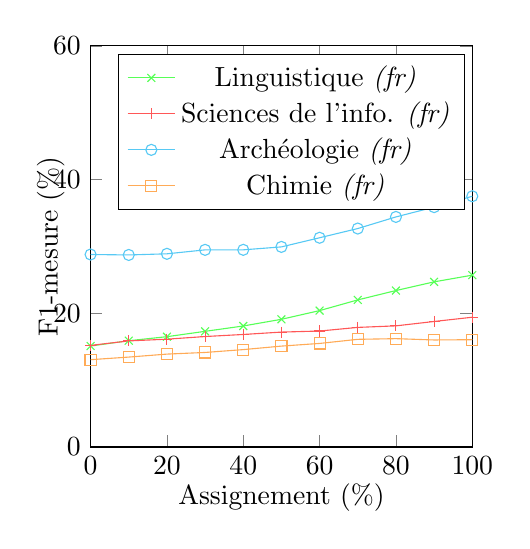
\begin{tikzpicture}
    \pgfkeys{/pgf/number format/.cd, fixed}
    \begin{axis}[x=0.0040\linewidth,
                 xtick={0, 20, ..., 100},
                 xmin=0,
                 xmax=100,
                 xlabel=Assignement (\%),
                 x label style={yshift=.34em},
                 y=0.007\linewidth,
                 ytick={0, 20, ..., 100},
                 ymin=0,
                 ymax=60,
                 ylabel=F1-mesure (\%),
                 y label style={yshift=-1.1em}]
      \addplot[green!66, mark=x] coordinates{
        (0, 15.1)
        (10, 15.9)
        (20, 16.5)
        (30, 17.3)
        (40, 18.1)
        (50, 19.1)
        (60, 20.4)
        (70, 22.0)
        (80, 23.4)
        (90, 24.7)
        (100, 25.7)
      };
      \addplot[red!66, mark=+] coordinates{
        (0, 15.1992)
        (10, 15.8659)
        (20, 16.1269)
        (30, 16.5223)
        (40, 16.8308)
        (50, 17.1875)
        (60, 17.3450)
        (70, 17.8887)
        (80, 18.1184)
        (90, 18.7733)
        (100, 19.4089)
      };
      \addplot[cyan!66, mark=o] coordinates{
        (0, 28.7887)
        (10, 28.7239)
        (20, 28.8927)
        (30, 29.4833)
        (40, 29.4880)
        (50, 29.9271)
        (60, 31.2943)
        (70, 32.6718)
        (80, 34.4101)
        (90, 35.8757)
        (100, 37.5003)
      };
      \addplot[orange!66, mark=square] coordinates{
        (0, 13.0605)
        (10, 13.4498)
        (20, 13.8944)
        (30, 14.1412)
        (40, 14.5673)
        (50, 15.0916)
        (60, 15.4902)
        (70, 16.1045)
        (80, 16.2055)
        (90, 16.0077)
        (100, 16.0506)
      };
      \legend{Linguistique \textit{(fr)}, Sciences de l'info. \textit{(fr)}, Archéologie \textit{(fr)}, Chimie \textit{(fr)}};
    \end{axis}
  \end{tikzpicture}
  \caption{Comportement de TopicCoRank en fonction du taux d'assignement
           \label{fig:assignment_variations}}
\end{figure}



        Enfin, nous réalisons une dernière expérience dans laquelle nous faisons
        varier la valeur du paramètre $\lambda$. Plus sa valeur est élevée, plus
        l'influence de la recommandation interne est forte et plus l'influence
        de la recommantation externe est faible. La
        figure~\ref{fig:lambda_variations_termith} montre le comportement de
        TopicCoRank lorsque nous faisons varier sa valeur de 0 à 1
        avec un pas de 0,1. En accord avec notre hypothèse que sujets et
        termes-clés du domaine doivent se recommander les uns les autres, les
        résultats montrent que les performances de TopicCoRank se dégradent au
        delà de $\lambda = 0,5$, valeur quasi-optimale.
        \begin{figure}[h!]
  \centering
  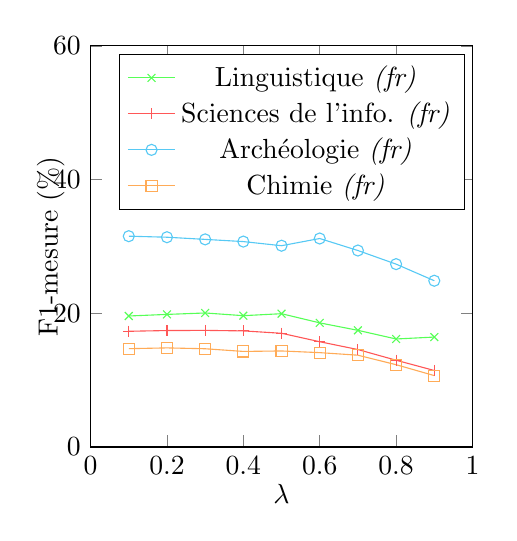
\begin{tikzpicture}
    \pgfkeys{/pgf/number format/.cd, fixed}
    \begin{axis}[x=0.4\linewidth,
                 xtick={0, 0.2, ..., 1.0},
                 xmin=0,
                 xmax=1.0,
                 xlabel=$\lambda$,
                 x label style={yshift=.34em},
                 y=0.007\linewidth,
                 ytick={0, 20, ..., 100},
                 ymin=0,
                 ymax=60,
                 ylabel=F1-mesure (\%),
                 y label style={yshift=-1.1em}]
      \addplot[green!66, mark=x] coordinates{
        (0.1, 19.5942)
        (0.2, 19.8314)
        (0.3, 20.0452)
        (0.4, 19.6420)
        (0.5, 19.9371)
        (0.6, 18.5649)
        (0.7, 17.4499)
        (0.8, 16.1558)
        (0.9, 16.4438)
      };
      \addplot[red!66, mark=+] coordinates{
        (0.1, 17.3100)
        (0.2, 17.4176)
        (0.3, 17.4420)
        (0.4, 17.3653)
        (0.5, 17.0094)
        (0.6, 15.7458)
        (0.7, 14.5758)
        (0.8, 12.9788)
        (0.9, 11.4421)
      };
      \addplot[cyan!66, mark=o] coordinates{
        (0.1, 31.5290)
        (0.2, 31.3748)
        (0.3, 31.0511)
        (0.4, 30.7214)
        (0.5, 30.1052)
        (0.6, 31.1819)
        (0.7, 29.3852)
        (0.8, 27.3498)
        (0.9, 24.8661)
      };
      \addplot[orange!66, mark=square] coordinates{
        (0.1, 14.7061)
        (0.2, 14.8227)
        (0.3, 14.6960)
        (0.4, 14.2947)
        (0.5, 14.3646)
        (0.6, 14.1136)
        (0.7, 13.7321)
        (0.8, 12.3091)
        (0.9, 10.6809)
      };
      \legend{Linguistique \textit{(fr)}, Sciences de l'info. \textit{(fr)}, Archéologie \textit{(fr)}, Chimie \textit{(fr)}};
    \end{axis}
  \end{tikzpicture}
  \caption{Comportement de TopicCoRank en fonction du taux d'assignement
           \label{fig:assignment_variations}}
\end{figure}


      
      \subsubsection{Évaluation de TopicCoRank hors domaines de spécialité}
      \label{subsubsec:main-domain_specific_keyphrase_annotation-supervised_automatic_keyphrase_annotation-evaluation-topiccorank_indepent_domains}
        Nous réalisons ici la même série d'évaluations précédentes, mais hors
        domaines de spécialités. L'objectif est de déterminer si TopicCoRank et
        ses hypothèses, fortement liées à notre étude de l'indexation manuelle
        en domaines de spécialités, se généralisent à tout type de documents.

        Le tableau~\ref{tab:topiccorank-comparison_results_general} montre les
        performances de TopicCoRank hors domaines de spécialités (\textsc{De}ft,
        SemEval et \textsc{Duc}) comparées à celles des méthodes de référence.
        Les résultats montrent de plus faibles performances qu'en domaines de
        spécialités. TopicCoRank échoue à améliorer TopicRank sur \textsc{De}ft,
        l'améliore légèrement sur SemEval et l'améliore significativement sur
        \textsc{Duc}, pour lequel nous utilisons des graphes de domaine très
        centrés sur le sujet d'actualité de chaque document de test.
        Contrairement à ce que nous observons en domaines de spécialités, c'est
        TopicCoRank qui est majoritairement le plus performant et c'est sa
        variante TopicCoRank$_\textnormal{assign.}$ qui est la moins
        performante. L'explication tient à la nature des termes-clés de
        référence de \textsc{De}ft et SemEval. Ceux-ci n'ont pas été produit à
        l'aide d'un vocabulaire contrôlé et les cinq principes sur lesquels nous
        fondons nos hypothèses ne sont pas respectés. La contrainte de
        conformité n'étant pas respectée, la nécessité de l'assignement n'est
        pas garantie~; la contrainte d'homogénéité n'étant pas respectée non
        plus, le graphe de domaine que nous construisons contient des
        termes-clés de référence redondants. La redondance des termes-clés de
        référence requiert une étape de normalisation. Celle-ci peut s'effectuer
        à l'aide de notre méthode de groupement en sujets.
        \begin{table}
          \centering
          %\resizebox{\linewidth}{!}{
            \begin{tabular}{l|ccc|ccc|ccc}
              \toprule
              \multirow{2}{*}{\textbf{Méthode}} & \multicolumn{3}{c|}{\textbf{\textsc{De}ft}} & \multicolumn{3}{c|}{\textbf{\textsc{Duc}}} & \multicolumn{3}{c}{\textbf{SemEval}}\\
              \cline{2-10}
              & P & R & F & P & R & F & P & R & F\\
              \hline
              \textsc{Tf-Idf} & 10,4 & 19,1 & 13,3 & 24,9 & 32,1 & 27,7$^{~~}$ & 13,6 & $~~$9,3 & 10,9\\
              TopicRank & \textbf{11,9} & \textbf{21,5} & \textbf{14,9} & 17,9 & 23,7 & 20,1$^{~~}$ & 16,6 & 11,5 & 13,5\\
              KEA++ & & & & & & & & &\\
              \overtabline
              \hline
              TopicCoRank$_\textnormal{extr.}$ & 10,1 & 19,1 & 13,0 & 24,6 & 35,5 & 27,2$^{~~}$ & 17,4 & 12,3 & 14,3\\
              TopicCoRank$_\textnormal{assign.}$ & $~~$6,8 & 12,8 & $~~$8,7 & 25,8 & 33,1 & 28,6$^{~~}$ & 11,8 & $~~$8,4 & $~~$9,7\\
              \hline
              TopicCoRank & $~~$8,7 & 16,2 & 11,2 & \textbf{28,2} & \textbf{36,3} & \textbf{31,3}$^\dagger$ & \textbf{17,6} & \textbf{12,5} & \textbf{14,5}\\
              \bottomrule
            \end{tabular}
          %}
        \caption[
          Résultat de l'extraction de dix termes-clés avec \textsc{Tf-Idf},
          TopicRank, \textsc{Kea++}, TopicCoRank$_\textnormal{\textit{extr.}}$,
          TopicCoRank$_\textnormal{\textit{assign.}}$ et TopicCoRank appliqués à
          \textsc{De}ft, SemEval et \textsc{Duc}
        ]{
          Résultat de l'extraction de dix termes-clés avec \textsc{Tf-Idf},
          TopicRank, \textsc{Kea++}, TopicCoRank$_\textnormal{\textit{extr.}}$,
          TopicCoRank$_\textnormal{\textit{assign.}}$ et TopicCoRank appliqués à
          \textsc{De}ft, SemEval et \textsc{Duc}. $\dagger$ indique une
          amélioration significative vis-à-vis des méthodes de référence, à
          0,001 pour le t-test de Student.
          \label{tab:topiccorank-comparison_results_general}}
        \end{table}

        La figure~\ref{fig:topiccorank-pr_curves_general} permet de comparer le
        comportement respectif des méthodes de référence, de TopicCoRank et de
        ses variantes. Contrairement aux domaines de spécialités, où TopicCoRank
        et ses variantes dominent les méthodes de référence, nous observons ici
        qu'aucune méthode dominante ne se dégage et, sauf sur \textsc{Duc}, il
        est difficile de statuer sur l'apport de TopicCoRank à TopicRank. Par
        ailleurs, le rappel maximal atteint par TopicCoRank n'excède, dans la
        plupart des cas, pas celui de \textsc{Tf-Idf}. TopicCoRank étant capable
        d'assigner des termes-clés qui n'occurrent pas dans le document, sont
        rappel maximal devrait être plus grand. Il existe deux raisons à ce
        problème. La première est aussi valable pour TopicRank. Comme les
        termes-clés candidats sont groupés en sujets et qu'un seul d'entre eux
        est extrait par sujet, si un terme-clé erroné est extrait d'un sujet
        contenant un terme-clé correct, alors le rappel maximal observable est
        plus faible que celui de \textsc{Tf-Idf}, qui peut extraire tous les
        candidats lorsque nous le lui demandons. La seconde raison nous
        intéresse particulièrement, car elle n'est pas observable en domaines de
        spécialités. En effet, le problème est aussi due à l'inconsistance des
        données d'entraînement pour représenter un \og{}domaine\fg{} de manière
        homogène et conforme à son vocabulaire. Les termes-clés employés dans
        les documents d'entraînement ne sont pas les mêmes que ceux employés
        pour les documents de test et l'assignement est donc inefficace.
        \begin{figure}[h!]
  \subfigure[\textsc{De}ft \textit{(fr)}]{
    \begin{tikzpicture}
      \pgfkeys{/pgf/number format/.cd, fixed}
      \begin{axis}[x=0.0057\linewidth,
                   xtick={0, 20, 40, ..., 100},
                   xmin=0,
                   xmax=60,
                   xlabel=rappel (\%),
                   x label style={yshift=.34em},
                   y=0.0057\linewidth,
                   ytick={0, 20, ..., 100},
                   ymin=0,
                   ymax=60,
                   ylabel=précision (\%),
                   y label style={yshift=-1.1em}]
        \addplot [green!66, mark=x] file {input/figure/data/deft_tfidf.csv};
        \addplot [red!66, mark=+] file {input/figure/data/deft_topicrank.csv};
        \addplot [orange!66, mark=square] file {input/figure/data/deft_topiccorank_extr.csv};
        \addplot [black!66, mark=triangle] file {input/figure/data/deft_topiccorank_assign.csv};
        \addplot [gray!66, mark=diamond] file {input/figure/data/deft_topiccorank.csv};
        %%%%%%%%%%%%%%%%%%%%%%%%%%%%%%%%%%%%%%%%%%%%%%%%%%%%%%%%%%%%%%%%%%%%%%%%
        \addplot [dotted, domain=35:100] {(50 * x) / ((2 * x) - 50)};
        \addplot [dotted, domain=25:100] {(40 * x) / ((2 * x) - 40)};
        \addplot [dotted, domain=15:100] {(30 * x) / ((2 * x) - 30)};
        \addplot [dotted, domain=10:100] {(20 * x) / ((2 * x) - 20)};
        \addplot [dotted, domain=5:100] {(10 * x) / ((2 * x) - 10)};
      \end{axis}
      \node at (4.85,3.6) [anchor=east] {\footnotesize{F=50,0}};
      \node at (4.85,2.6) [anchor=east] {\footnotesize{F=40,0}};
      \node at (4.85,1.8) [anchor=east] {\footnotesize{F=30,0}};
      \node at (4.85,1.15) [anchor=east] {\footnotesize{F=20,0}};
      \node at (4.85,0.6) [anchor=east] {\footnotesize{F=10,0}};
    \end{tikzpicture}
  }
  \subfigure[Semeval \textit{(en)}]{
    \begin{tikzpicture}
      \pgfkeys{/pgf/number format/.cd, fixed}
      \begin{axis}[x=0.0057\linewidth,
                   xtick={0, 20, 40, ..., 100},
                   xmin=0,
                   xmax=60,
                   xlabel=rappel (\%),
                   x label style={yshift=.34em},
                   y=0.0057\linewidth,
                   ytick={0, 20, ..., 100},
                   ymin=0,
                   ymax=60,
                   ylabel=précision (\%),
                   y label style={yshift=-1.1em}]
        \addplot [green!66, mark=x] file {input/figure/data/semeval_tfidf.csv};
        \addplot [red!66, mark=+] file {input/figure/data/semeval_topicrank.csv};
        \addplot [orange!66, mark=square] file {input/figure/data/semeval_topiccorank_extr.csv};
        \addplot [black!66, mark=triangle] file {input/figure/data/semeval_topiccorank_assign.csv};
        \addplot [gray!66, mark=diamond] file {input/figure/data/semeval_topiccorank.csv};
        %%%%%%%%%%%%%%%%%%%%%%%%%%%%%%%%%%%%%%%%%%%%%%%%%%%%%%%%%%%%%%%%%%%%%%%%
        %\addplot [dotted, domain=35:100] {(50 * x) / ((2 * x) - 50)};
        %\addplot [dotted, domain=25:100] {(40 * x) / ((2 * x) - 40)};
        \addplot [dotted, domain=15:100] {(30 * x) / ((2 * x) - 30)};
        \addplot [dotted, domain=10:100] {(20 * x) / ((2 * x) - 20)};
        \addplot [dotted, domain=5:100] {(10 * x) / ((2 * x) - 10)};
        %%%%%%%%%%%%%%%%%%%%%%%%%%%%%%%%%%%%%%%%%%%%%%%%%%%%%%%%%%%%%%%%%%%%%%%%
        \legend{\textsc{Tf-Idf}, TopicRank, TopicCoRank$_\textnormal{extr.}$,
                TopicCoRank$_\textnormal{assign.}$, TopicCoRank};        
      \end{axis}
      %\node at (4.85,3.6) [anchor=east] {\footnotesize{F=50,0}};
      %\node at (4.85,2.6) [anchor=east] {\footnotesize{F=40,0}};
      \node at (4.85,1.8) [anchor=east] {\footnotesize{F=30,0}};
      \node at (4.85,1.15) [anchor=east] {\footnotesize{F=20,0}};
      \node at (4.85,0.6) [anchor=east] {\footnotesize{F=10,0}};
    \end{tikzpicture}
  }
  \subfigure[\textsc{Duc} \textit{(en)}]{
    \begin{tikzpicture}
      \pgfkeys{/pgf/number format/.cd, fixed}
      \begin{axis}[x=0.0057\linewidth,
                   xtick={0, 20, 40, ..., 100},
                   xmin=0,
                   xmax=60,
                   xlabel=rappel (\%),
                   x label style={yshift=.34em},
                   y=0.0057\linewidth,
                   ytick={0, 20, ..., 100},
                   ymin=0,
                   ymax=60,
                   ylabel=précision (\%),
                   y label style={yshift=-1.1em}]
        \addplot [green!66, mark=x] file {input/figure/data/duc_tfidf.csv};
        \addplot [red!66, mark=+] file {input/figure/data/duc_topicrank.csv};
        \addplot [orange!66, mark=square] file {input/figure/data/duc_topiccorank_extr.csv};
        \addplot [black!66, mark=triangle] file {input/figure/data/duc_topiccorank_assign.csv};
        \addplot [gray!66, mark=diamond] file {input/figure/data/duc_topiccorank.csv};
        %%%%%%%%%%%%%%%%%%%%%%%%%%%%%%%%%%%%%%%%%%%%%%%%%%%%%%%%%%%%%%%%%%%%%%%%
        \addplot [dotted, domain=35:100] {(50 * x) / ((2 * x) - 50)};
        \addplot [dotted, domain=25:100] {(40 * x) / ((2 * x) - 40)};
        \addplot [dotted, domain=15:100] {(30 * x) / ((2 * x) - 30)};
        \addplot [dotted, domain=10:100] {(20 * x) / ((2 * x) - 20)};
        \addplot [dotted, domain=5:100] {(10 * x) / ((2 * x) - 10)};
      \end{axis}
      \node at (4.85,3.6) [anchor=east] {\footnotesize{F=50,0}};
      \node at (4.85,2.6) [anchor=east] {\footnotesize{F=40,0}};
      \node at (4.85,1.8) [anchor=east] {\footnotesize{F=30,0}};
      \node at (4.85,1.15) [anchor=east] {\footnotesize{F=20,0}};
      \node at (4.85,0.6) [anchor=east] {\footnotesize{F=10,0}};
    \end{tikzpicture}
  }
  \caption{Courbes de rappel-précision de \textsc{Tf-Idf}, TopicRank,
           TopicCoRank$_\textnormal{extr.}$, TopicCoRank$_\textnormal{assign.}$
           et TopicCoRank appliqués à \textsc{De}ft, SemEval et \textsc{Duc}
           \label{fig:topiccorank-pr_curves}}
\end{figure}



        Comme pour l'évaluation en domaines de spécialités, le
        tableau~\ref{tab:assignment_ratio_general} reporte les taux d'extraction
        et d'assignement réalisés par TopicCoRank sur \textsc{De}ft, SemEval et
        \textsc{Duc}. Ceux-ci montrent aussi que les deux catégories
        d'indexation sont réalisées conjointement, cette fois-ci sans
        prédominance de l'une face à l'autre.
        \begin{table}[h]
          \centering
          \begin{tabular}{l|c|c}
              \toprule
              & Extraction (\%) & Assignement (\%)\\
              \hline
              \textsc{De}ft \textit{(fr)} & 48,4 & 51,6\\
              SemEval \textit{(en)} & 61,4 & 38,6\\
              \textsc{Duc} \textit{(en)} & 46,9 & 53,1\\
              \bottomrule
          \end{tabular}
          \caption{Taux moyens d'extraction et d'assignement réalisés par
                   TopicCoRank pour les collections Termith
                   \label{tab:assignment_ratio_general}}
        \end{table}

        La figure~\ref{fig:assignment_variations_general} montrent les
        performances de TopicCoRank lorsque nous forçons le taux d'assignement,
        de 0~\% à 100~\% avec un pas de 10~\%. Contrairement à la courbe de
        performances en domaines de spécialités, celle de TopicCoRank hors
        domaines de spécialités est croissante puis décroissante pour \text{Duc}
        et décroissante pour \textsc{De}ft et SemEval. Cela signifie que
        l'ordonnancement des termes-clés du domaine est moins efficace hors
        domaines de spécialités. Il est toutefois intéressant de noter que, sur
        \textsc{Duc}, le taux d'assignement effectué par TopicCoRank sans que
        nous ne le forcions est proche de sa valeur optimal.
        \begin{figure}[h!]
  \centering
  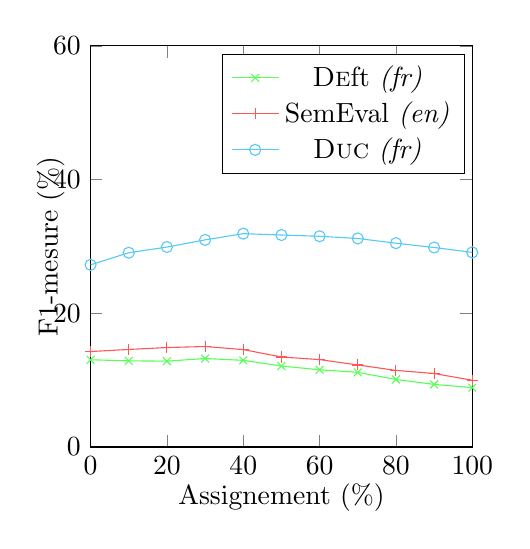
\begin{tikzpicture}
    \pgfkeys{/pgf/number format/.cd, fixed}
    \begin{axis}[x=0.0040\linewidth,
                 xtick={0, 20, ..., 100},
                 xmin=0,
                 xmax=100,
                 xlabel=Assignement (\%),
                 x label style={yshift=.34em},
                 y=0.007\linewidth,
                 ytick={0, 20, ..., 100},
                 ymin=0,
                 ymax=60,
                 ylabel=F1-mesure (\%),
                 y label style={yshift=-1.1em}]
      \addplot[green!66, mark=x] coordinates{
        (0, 13.0470)
        (10, 12.8868)
        (20, 12.8409)
        (30, 13.2342)
        (40, 12.9643)
        (50, 12.1117)
        (60, 11.5492)
        (70, 11.1649)
        (80, 10.1043)
        (90, 9.3643)
        (100, 8.8794)
      };
      \addplot[red!66, mark=+] coordinates{
        (0, 14.2790)
        (10, 14.5905)
        (20, 14.8776)
        (30, 15.0293)
        (40, 14.5713)
        (50, 13.4616)
        (60, 13.0731)
        (70, 12.2721)
        (80, 11.4582)
        (90, 10.9929)
        (100, 9.9841)
      };
      \addplot[cyan!66, mark=o] coordinates{
        (0, 27.2447)
        (10, 29.0553)
        (20, 29.9039)
        (30, 30.9763)
        (40, 31.9071)
        (50, 31.7050)
        (60, 31.5150)
        (70, 31.1887)
        (80, 30.4816)
        (90, 29.8382)
        (100, 29.1068)
      };
      \legend{\textsc{De}ft \textit{(fr)}, SemEval \textit{(en)}, \textsc{Duc} \textit{(fr)}};
    \end{axis}
  \end{tikzpicture}
  \caption{Comportement de TopicCoRank en fonction du taux d'assignement
           \label{fig:assignment_variations}}
\end{figure}



        La figure~\ref{fig:lambda_variations_general} montre le comportement de
        TopicCoRank lorsque nous faisons varier la valeur de $\lambda$ de 0 à 1
        avec un pas de 0,1. Sur \textsc{Duc}, comme en domaines des spécialités,
        l'indexation par termes-clés est meilleure lorsque l'ordonnancement est
        fortement influencé par la recommandation externe que lorsqu'il ne l'est
        pas. Sur \textsc{De}ft et SemEval, c'est l'inverse~: l'indexation par
        termes-clés est plus performante lorsque l'ordonnancement au sein de
        chaque graphe n'est que très faiblement influencé par l'ordonnancement
        au sein de l'autre. Comme observé précédemment, les données
        d'entraînement sont telles que le graphe du domaine est innefficace,
        voir contre-productif.
        \begin{figure}[t]
  \centering
  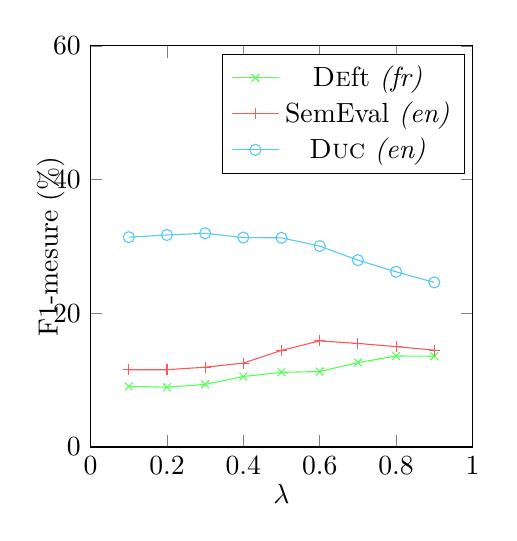
\begin{tikzpicture}
    \pgfkeys{/pgf/number format/.cd, fixed}
    \begin{axis}[x=0.4\linewidth,
                 xtick={0, 0.2, ..., 1.0},
                 xmin=0,
                 xmax=1.0,
                 xlabel=$\lambda$,
                 x label style={yshift=.34em},
                 y=0.007\linewidth,
                 ytick={0, 20, ..., 100},
                 ymin=0,
                 ymax=60,
                 ylabel=F1-mesure (\%),
                 y label style={yshift=-1.1em}]
      \addplot[green!66, mark=x] coordinates{
        (0.1, 9.0736)
        (0.2, 8.9392)
        (0.3, 9.3693)
        (0.4, 10.5436)
        (0.5, 11.1626)
        (0.6, 11.2902)
        (0.7, 12.6269)
        (0.8, 13.6109)
        (0.9, 13.5765)
      };
      \addplot[red!66, mark=+] coordinates{
        (0.1, 11.5509)
        (0.2, 11.5618)
        (0.3, 11.9382)
        (0.4, 12.5558)
        (0.5, 14.4539)
        (0.6, 15.8712)
        (0.7, 15.4920)
        (0.8, 15.0102)
        (0.9, 14.4863)
      };
      \addplot[cyan!66, mark=o] coordinates{
        (0.1, 31.3789)
        (0.2, 31.7112)
        (0.3, 31.9601)
        (0.4, 31.3222)
        (0.5, 31.2842)
        (0.6, 30.0481)
        (0.7, 27.9426)
        (0.8, 26.1973)
        (0.9, 24.6206)
      };
      \legend{\textsc{De}ft \textit{(fr)}, SemEval \textit{(en)}, \textsc{Duc} \textit{(en)}};
    \end{axis}
  \end{tikzpicture}
  \caption{Performance de TopicCoRank, appliqué à \textsc{De}ft, SemEval et
           \textsc{Duc}, lorsque le paramètre $\lambda$ varie
           \label{fig:lambda_variations_general}}
\end{figure}



    \subsection{Analyse des sorties de TopicCoRank}
    \label{subsec:main-domain_specific_keyphrase_annotation-supervised_automatic_keyphrase_annotation-error_analysis}
      Dans cette section, nous analysons les termes-clés corrects (vrais
      positifs) et incorrects (faux positifs) issus du graphe du domaine des
      collections Termith.

      \subsubsection{Analyse des vrais positifs}
      \label{subsec:main-domain_specific_keyphrase_annotation-supervised_automatic_keyphrase_annotation-error_analysis-true_positives}
        Parmi les termes-clés assignés, ceux qui sont corrects sont en grande
        partie présents dans le contenu du document. Ils sont directement
        connectés aux sujets du document et leur importance respective évolue de
        manière similaire. Il est fréquent qu'un terme-clé candidat d'un sujet
        soit extrait en même temps qu'un terme-clé de référence du domaine
        connecté à ce sujet. Dans cette situation, nous distinguons deux cas de
        figure~: un seul terme-clé est produit, car le terme-clé extrait et
        celui assigné sont les mêmes~; deux termes-clés corrects complémentaires
        sont produits, car le terme-clé extrait et celui assigné ne sont pas les
        mêmes.
        
        Il est plus difficile pour les termes-clés de référence du domaine
        connectés indirectement aux sujets du document d'émerger. Nous observons
        toutefois l'émergence de noms de disciplines (par exemple \og{}analyse
        du discours\fg{} en linguistique) et de termes-clés génériques (par
        exemple \og{}français\fg{} en linguistique, ou encore \og{}Europe\fg{}
        en archéologie). Nous observons dans les données Termith des cadres
        d'études très récurrents (par exemple, la langue française, en
        linguistique, ou des fouilles de sites européens, en archéologie) et, de
        ce fait, certains termes-clés génériques sont très fréquemment utilisés
        (\og{}français\fg{} apparaît dans 48,9~\% des documents de linguistique
        et \og{}Europe\fg{} apparaît dans 52,5~\% des documents d'archéologie).
        \TODO{plus d'exemples}

      \subsubsection{Analyse des faux positifs}
      \label{subsec:main-domain_specific_keyphrase_annotation-supervised_automatic_keyphrase_annotation-error_analysis-false_positives}
        Les termes-clés génériques évoqués dans l'analyse des vrais positifs
        sont aussi sources d'erreurs. En effet, comme ils sont associés à un
        nombre conséquent de documents d'entraînement, ils sont connectés à
        beaucoup d'autres termes-clés du domaine et gagnent donc de l'importance
        quelque soit le document. Pour l'exemple du terme-clé \og{}français\fg{}
        en linguistique, nous observons des documents qui traitent de l'arabe
        mais, parce que les termes techniques employés sont les mêmes
        (\og{}syntaxe\fg{}, \og{}sémantique\fg{}, etc.), \og{}français\fg{} est
        assigné.

        Enfin, nous observons quelques problèmes liés à la présence de
        termes-clés de référence redondants, c'est-à-dire des synonymes. C'est
        le cas, par exemple, du terme-clé \og{}rite funéraire\fg{}, qui fait
        parti du vocabulaire contrôlé d'archéologie, et qui est parfois remplacé
        par le terme-clé \og{}pratique funéraire\fg{}, qui ne fait pas partie du
        vocabulaire contrôlé d'archéologie. TopicCoRank échoue parfois parce
        qu'il a assigné l'un alors que c'était l'autre qu'il fallait trouver.

    \subsection{Bilan}
    \label{subsec:main-domain_specific_keyphrase_annotation-supervised_automatic_keyphrase_annotation-conclusion}
      Nous avons présenté TopicCoRank, une extension de la méthode TopicRank.
      Proposée dans le but de simuler le comportement d'un indexeur
      professionnel, cette extension apporte à TopicRank la capacité à assigner
      des termes-clés. Pour ce faire, TopicCoRank utilise les termes-clés de
      référence des documents d'entraînement comme vocabulaire contrôlé, crée un
      graphe dont chaque n\oe{}ud est une entrée du vocabulaire connecté aux
      autres lorsqu'ils sont termes-clés d'un même document, puis unifie ce
      graphe au graphe de sujets de TopicRank.

      Les résultats de l'évaluation de TopicCoRank en domaines de spécialités
      montrent une amélioration significative vis-à-vis de l'état de l'art. Ceux
      hors domaines de spécialités sont moins probants. Les hypothèses que nous
      faisons en proposant TopicCoRank sont fondées sur une étude de
      l'indexation manuelle en domaines de spécialités qui ne sont pas
      directement généralisables à tout type de documents.

  %-----------------------------------------------------------------------------

  \section{Évaluation manuelle en domaines de spécialités}
  \label{sec:main-domain_specific_keyphrase_annotation-manual_evaluation}
    L'évaluation manuelle des méthodes d'indexation par termes-clés consiste à
    faire valider par un ou plusieurs évaluateurs humains les termes-clés
    proposés par une méthodes automatique. Parce qu'elle est coûteuse, cette
    évaluation est quasi-systématiquement remplacée par une évaluation
    automatique, d'après le paradigme de l'évaluation \og{}à la Crandield\fg{},
    comme nous l'avons fait dans nos travaux. Néanmoins, ce paradigme
    d'évaluation n'est pas adapté à la tâche d'indexation par termes-clés, car
    il ne considère qu'une seule et unique réponse exacte, c'est-à-dire un seul
    et unique ensemble correct de termes-clés, alors que certaines variantes
    d'ensembles de termes-clés sont acceptables (\TODO{exemple}). Ayant à notre
    disposition des indexeurs professionnels de l'Inist, nous réalisons donc une
    campagne d'évaluation manuelle.

    Dans la suite, nous présentons le protocole d'évaluation et les métriques
    que nous avons proposés, puis nous analysons les premiers résultats de la
    campagne d'évaluation manuelle de TopicRank et d'une méthode de référence en
    domaine de spécialités avec la collection de linguistique Termith.

    \subsection{Protocole d'évaluation manuelle}
    \label{subsec:main-automatic_evaluation_of_keyphrase_annotation-methodology-evaluation_protocol}
      L'évaluation manuelle concerne dix termes-clés extraits et/ou assignés par
      chaque méthode d'indexation par termes-clés. Le protocole que nous
      proposons permet d'évaluer deux aspects de l'indexation automatique par
      termes-clés~:
      \begin{enumerate}
        \item{Pertinence (validité)~: chaque terme-clé fourni par la méthode
              d'indexation automatique par termes-clés est-il important pour la
              compréhension du contenu principal du document~?}
        \item{Silence~: quel est le degré d'importance des informations perdues
              entre les termes-clés de référence et les termes-clés fournis par
              la méthode d'indexation automatique par termes-clés~?}
      \end{enumerate}
      L'évaluation de la pertinence s'intéresse au même aspect que l'évaluation
      automatique~: le nombre de termes-clés corrects doit être maximisé et le
      nombre d'erreurs minimisé pour obtenir la meilleure performance.
      L'évaluation du silence s'intéresse à un aspect qui lui est propre. Elle a
      une dimension plus sémantique~: les termes-clés corrects dont
      l'information est la plus capitale pour la compréhension du contenu
      principal du document doivent être priorisés pour obtenir la meilleure
      performance.

      Afin de minimiser les problèmes d'ambiguïté et de subjectivité de certains
      cas de figure, la pertinence et le silence sont évalués sur une échelle à
      trois valeurs~: une valeur représentant le succès, une autre l'échec et
      une dernière le cas intermédiaire.

      \subsubsection{Évaluation de la pertinence}
      \label{subsubsec:main-automatic_evaluation_of_keyphrase_annotation-methodology-evaluation_protocol-relevancy}
        Pour évaluer la pertinence d'un terme-clé fourni par une méthode
        d'indexation par termes-clés, l'évaluateur doit lui attribuer un score
        sur une échelle de 0 à 2. Ce score distingue les termes-clés incorrects
        (0), les termes-clés corrects (2) et les variantes de ces derniers (1).

        Pour permettre une étude précise de cette évaluation, les indexeurs
        professionnels doivent indiquer la forme préférée des termes-clés
        auxquels ils donnent un score de 1 (variantes). Une variante peut faire
        référence à deux catégories de formes préférées, qui induisent deux
        raisonnements~:
        \begin{itemize}
          \item{variante d'un terme-clé déjà fourni (score de
                2)~$\Rightarrow$~la méthode d'indexation par termes-clés fourni
                des termes-clés redondants~; \TODO{exemple sur capture}}
          \item{variante d'un terme-clé non fourni mais présent dans le
                texte~$\Rightarrow$~la méthode d'indexation par termes-clés
                identifie correctement les sujets importants du document, mais
                peine à trouver la forme la plus appropriée pour les
                représenter. \TODO{exemple sur capture}}
        \end{itemize}

        Lorsque la forme préférée n'est pas présente dans le document, nous
        estimons que la méthode d'indexation a fourni un terme-clé correct,
        auquel cas il se voit attribuer le score de 2. Les formes variantes
        résultant d'un accord en nombre (pluriel) obtiennent aussi un score de
        2, lorsque la forme normalisée (singulier) ne se trouve pas parmi les
        termes-clés fournis.

      \subsubsection{Évaluation du silence}
      \label{subsubsec:main-automatic_evaluation_of_keyphrase_annotation-methodology-evaluation_protocol-silence}
        Pour évaluer le silence, l'évaluateur doit attribuer à chaque terme-clé
        de référence un score indiquant le degré d'importance de l'information
        qu'il véhicule et qui n'est pas capturée par les termes-clés fournis par
        une méthode d'indexation par termes-clés. Sur une échelle de 0 à 2, ce
        score permet d'indiquer s'il n'y pas de perte d'information (0), si
        l'information perdue est capitale (2) ou si elle est secondaire (1).
        Lorsqu'un terme-clé de référence obtient un score de 0, cela signifie
        soit qu'il fait partie des termes-clés fournis par la méthode
        d'indexation par termes-clés, soit que l'indexeur juge qu'il ne devrait
        pas être un terme-clé de référence, c'est-à-dire une erreur parmi les
        termes-clés de référence.

        Une perte d'information est jugée secondaire (score de 1) dans deux
        cas de figure~:
        \begin{itemize}
          \item{terme-clé de référence secondaire~: le terme-clé de référence
                n'apporte pas l'information la plus importante~;
                \TODO{exemple sur capture}}
          \item{terme-clé de référence générique~: le terme-clé de référence
                n'est pas suffisamment spécifique au contenu du document, il a
                un usage classificatoire~; \TODO{exemple sur capture}}
        \end{itemize}
        Afin de minimiser les pertes d'informations dues à des termes-clés de
        référence qui ne sont pas présents dans le document, les évaluateurs
        leur attribuent un score de 1.

    \subsection{Évaluation manuelle des méthodes proposées}
    \label{subsec:main-domain_specific_keyphrase_annotation-manual_evaluation-analysis}
      Dans cette section, nous analysons l'évaluation manuelle de TopicRank,
      %TopicCoRank, d'une méthode de référence non supervisée, \textsc{Tf-Idf},
      %et d'une méthode de référence supervisée, \textsc{Kea}. L'évaluation est
      et d'une méthode de référence, \textsc{Tf-Idf}. L'évaluation est
      effectuée par un indexeur professionnel, sur la collection de linguistique
      Termith.

      Dans un premier temps, nous analysons l'évaluation manuelle de TopicRank
      et la comparons à celle de \textsc{Tf-Idf}, puis, dans un second temps,
      nous analysons l'évaluation manuelle de TopicCoRank et la comparons à
      celle de \textsc{Kea}\footnote{La raison pour laquelle les évaluations
      manuelles sont réalisées sur \textsc{Kea} et non pas \textsc{Kea++} est
      temporelle. L'évaluation manuelle étant coûteuse, nous n'avons pas pu
      la réitérer avec \textsc{Kea++}.}.

      \subsubsection{Analyse de TopicRank}
      \label{subsubsec:main-domain_specific_keyphrase_annotation-manual_evaluation-analysis-topicrank}
        Le
        tableau~\ref{tab:main-automatic_evaluation_of_keyphrase_annotation-results-topicrank-pertinence_score_ratio}
        montre les scores de pertinence moyens de chaque méthode. Pour le score
        de 1, qui indique qu'un terme-clé est un forme variante, nous
        distinguons le cas où la variante est redondante du cas où elle ne l'est
        pas. Globalement, nous observons que TopicRank est meilleur que
        \textsc{Tf-Idf}. TopicRank fournit plus de termes-clés pertinents que
        \textsc{Tf-Idf}, mais fait aussi plus d'erreurs. Les termes-clés ayant
        un score de 1 donnent un explication intéressante à cette
        contradiction~: \textsc{Tf-Idf} à une forte tendance à extraire des
        termes-clés redondants, c'est-à-dire des termes-clés variantes de
        termes-clés déjà extrait, alors que TopicRank remplit presque son
        objectif de ne pas extraire de termes-clés redondants, avec seulement
        0,9~\% de termes-clés redondants.
        \begin{table}[h!]
          \centering
          \begin{tabular}{l|c|c|c|c}
            \toprule
            \multirow{2}{*}{\textbf{Méthode}} & \multirow{2}{*}{\textbf{0}} & \multicolumn{2}{c|}{\textbf{1}} & \multirow{2}{*}{\textbf{2}}\\
            \cline{3-4}
            & & \multicolumn{1}{p{.175\linewidth}|}{\centering{}redondant} & \multicolumn{1}{p{.175\linewidth}|}{\centering{}non redondant} &\\
            \hline
            \textsc{Tf-Idf} & \textbf{53,8~\%} & 6,8~\% & 4,2~\% & 35,3~\%\\
            TopicRank & 56,3~\% & \textbf{0,9~\%} & \textbf{5,7~\%} & \textbf{37,1~\%}\\
            \bottomrule
          \end{tabular}
          \caption{Taux de termes-clés avec un score de 0, de 1 ou de 2 pour
                   l'évaluation de la pertinence de \textsc{Tf-Idf} et de
                   TopicRank
                   \label{tab:main-automatic_evaluation_of_keyphrase_annotation-results-topicrank-pertinence_score_ratio}}
        \end{table}

        Les résultats présentés dans le
        tableau~\ref{tab:main-automatic_evaluation_of_keyphrase_annotation-results-topicrank-pertinence_score_ratio}
        sont contraires à ceux de l'évaluation automatique, puisque c'est ici
        TopicRank qui est meilleur que \textsc{Tf-Idf} sur les documents de
        linguistique. Afin de mieux observer la différence entre l'évaluation
        manuelle et l'évaluation automatique, nous calculons la précision (P),
        le rappel (R) et la f-mesure (f1-mesure, F) résultantes de l'évaluation
        manuelle et les comparons aux résultats automatiques que nous avons
        montré dans le tableau~\ref{tab:resultats_inist}
        (page~\pageref{tab:resultats_inist}). Pour calculer ces performances,
        les termes-clés ayant un score de 2 sont considérés corrects, de même
        que ceux ayant un score de 1 non redondants. Les résultats de
        l'évaluation manuelle comparés à ceux de l'évaluation automatique sont
        présentés dans le
        tableau~\ref{tab:main-automatic_evaluation_of_keyphrase_annotation-results-topicrank-prf}
        . La difficulté d'évaluer automatiquement la tâche d'indexation par
        termes-clés se confirme. Avec l'évaluation manuelle, les conclusions ne
        sont pas les mêmes, puisque de manière automatique TopicRank est moins
        performant que \textsc{Tf-Idf} alors qu'il est plus performant selon
        l'évaluation manuelle. Nous observons aussi un écart conséquent entre
        les performances évaluées manuellement et celles évaluées
        automatiquement. Le gain d'environ 20 points attestent le pessimisme de
        l'évaluation automatique.
        \begin{table}[h!]
          \centering
          \begin{tabular}{l|ccc|ccc}
            \toprule
            \multirow{2}{*}{\textbf{Méthode}} & \multicolumn{3}{c|}{\textbf{Évaluation manuelle}} & \multicolumn{3}{c}{\textbf{Évaluation automatique}}\\
            \cline{2-7}
            & P & R & F & P & R & F\\
            \hline
            \textsc{Tf-Idf} & 39,5 & 29,7 & 33,5 & \textbf{13,0} & \textbf{15,4} & \textbf{13,9}\\
            TopicRank & \textbf{42,8} & \textbf{32,2} & \textbf{36,2} & 11,2 & 13,1 & 11,9\\
            \bottomrule
          \end{tabular}
          \caption[
            Performances de \textsc{Tf-Idf} et de TopicRank en termes de
            précision, de rappel et de f-mesure
          ]{
            Performances de \textsc{Tf-Idf} et de TopicRank en termes de
            précision (P), de rappel (R) et de f-mesure (F)
            \label{tab:main-automatic_evaluation_of_keyphrase_annotation-results-topicrank-prf}}
        \end{table}
      
        ~\\Enfin, le
        tableau~\ref{tab:main-automatic_evaluation_of_keyphrase_annotation-results-topicrank-silence_score_ratio}
        montre les scores de silence attribués en moyenne par méthode. D'après
        la description donnée pour chacun des scores, la méthode qui capture le
        plus d'information est celle qui maximise le nombre de termes-clés de
        référence ayant un score de silence 0 et qui minimise ceux ayant un
        score de 1 et de 2. Nous observons donc que TopicRank couvre mieux le
        contenu principal des documents que \textsc{Tf-Idf}. Parce que TopicRank
        groupe les termes-clés candidats en sujets et n'extrait qu'un seul
        terme-clé par sujet, il y a moins de redondance parmi les termes-clés
        qu'il extrait (cf
        tableau~\ref{tab:main-automatic_evaluation_of_keyphrase_annotation-results-topicrank-pertinence_score_ratio})
        et le nombre de sujets couverts est donc meilleur.
        \begin{table}[h!]
          \centering
          \begin{tabular}{l|c|c|c}
            \toprule
            \textbf{Méthode} & \textbf{0} & \textbf{1} & \textbf{2}\\
            \hline
            \textsc{Tf-Idf} & 31,4~\% & 48,5~\% & 20,1~\%\\
            TopicRank & \textbf{35,0~\%} & \textbf{48,3~\%} & \textbf{16,8~\%}\\
            \bottomrule
          \end{tabular}
          \caption{Taux de termes-clés de référence avec un score de 0, de 1 ou
                   de 2 pour l'évaluation du silence de \textsc{Tf-Idf} et de
                   TopicRank
                   \label{tab:main-automatic_evaluation_of_keyphrase_annotation-results-topicrank-silence_score_ratio}}
        \end{table}

%      \subsubsection{Analyse de TopicCoRank}
%      \label{subsubsec:main-domain_specific_keyphrase_annotation-manual_evaluation-analysis-topiccorank}
%        \TODO{\dots}

    \subsection{Bilan}
    \label{subsec:main-domain_specific_keyphrase_annotation-manual_evaluation-conclusion}
      Nous avons réalisé une campagne d'évaluation manuelle de nos travaux en
      domaine de spécialités, avec la collection de linguistique Termith. Pour
      cette campagne, nous avons proposé un protocole d'évaluation et des
      métriques permettant de capturer deux aspects de l'indexation par
      termes-clés~: la pertinence des termes-clés extraits/assignés et leur
      silence, c'est-à-dire la quantité d'information importante qu'ils ne
      capturent pas. Contrairement au premier, qui est similaire à ce qu'évalue
      un système automatique, le dernier aspect permet d'évaluer les termes-clés
      d'un point de vu sémantique, jamais considéré auparavant.

      Les résultats montrent que, contrairement à ce que montrait l'évaluation
      automatique, TopicRank effectue une indexation par termes-clés de
      meilleure qualité que celle de \textsc{Tf-Idf}. TopicRank extrait peu de
      termes-clés redondants et couvre mieux le document, en partie grâce à son
      groupement des termes-clés candidats en sujets.

  %-----------------------------------------------------------------------------

  \section{Conclusion}
  \label{sec:main-domain_specific_keyphrase_annotation-conclusion}
    Nous nous sommes intéressé à l'indexation automatique par termes-clés en
    domaines de spécialités. Nous avons tout d'abord présenté l'indexation
    manuelle réalisée par des indexeurs professionnels dans ce contexte, nous
    avons ensuite proposé une nouvelle méthode automatique se rapprochant le
    plus possible de cette indexation, puis nous avons présenté les premiers
    résultats d'une campagne d'évaluation manuelle que nous avons réalisé avec
    des indexeurs professionnels.

    Contrairement aux méthodes d'indexation automatique, l'indexation manuelle
    n'est pas divisée entre extraction et assignement. L'indexation manuelle en
    domaines de spécialités préfère l'assignement, car cela permet une
    indexation homogène des documents d'un même domaine et une conformité
    vis-à-vis du vocabulaire spécialisé du domaine. Elle a aussi besoin de
    l'extraction, afin de fournir des termes-clés très spécifiques au document,
    ainsi que pour y identifier d'éventuels nouveaux concepts.

    Pour remédier à la fracture entre extraction et assignement en indexation
    automatique par termes-clés, nous proposons TopicCoRank. Conçu sur la base
    de TopicRank, TopicCoRank utilise les données d'entraînement pour présenter
    le domaine avec un graphe unifiié à celui des sujets. Cette unification
    permet d'améliorer l'ordonnancement des sujets, en tenant compte de leurs
    relations avec le domaine, et d'assigner des termes-clés, en puisant dans le
    domaine. À notre connaissance, TopicCoRank est la seule méthode qui réalise
    conjointement extraction et assignement.

    Pour valider les deux méthodes TopicRank et TopicCoRank, nous avons réalisé
    une campagne d'évaluation manuelle en domaines de spécialités. Le protocole
    d'évaluation que nous avons proposé permet d'évaluer chaque méthode selon le
    degré de pertinence des termes-clés qu'elle propose et selon le degré
    d'information qui lui échape. Les résultats de l'évaluation manuelle de
    TopicRank son plus encourageant que ceux de l'évaluation automatique. Ils
    montrent que TopicRank est en réalité plus performant que \textsc{Tf-Idf},
    en partie parce qu'il couvre mieux les sujets du document grâce à son
    groupement en sujets des termes-clés candidats. Au delà de cela, cette
    campagne a montré les limites de l'évaluation automatique, qui suit un
    paradigme trop strict pour la tâche d'indexation par termes-clés. Parce que
    l'évaluation manuelle est trop coûteuse pour être systématiquement mise en
    \oe{}uvre, il est donc important de s'intéresser de plus près aux méthodes
    d'évaluation automatique. Toutes les étapes de notre campagne seront donc
    rendues disponibles gratuitement à toute la communauté scientifique. Cette
    disponibilité permettra d'évaluer de nouvelles méthodes d'évaluation, en
    vérifiant leur corrélation avec l'évaluation manuelle des indexeurs
    professionnels.


  %\chapter{Évaluations manuelles}
\label{chap:main-manuelle_evaluation_of_keyphrase_annotation}
  \chaptercite{
    The performance of most keyphrase extraction algorithms is [automatically]
    evaluated by comparing whether the extracted keyphrases exactly match the
    human assigned gold standard keyphrases. However, this is known to
    underestimate performance.
  }{
    \newcite{zesch2009rprecision}
  }

  \section{Introduction}
  \label{sec:main-automatic_evaluation_of_keyphrase_annotation-introduction}
    Pour évaluer les performances d'une méthode d'indexation automatique par
    termes-clés et la comparer aux autres méthodes, il est courant d'utiliser un
    système d'évaluation automatique. Un tel système utilise un jugement de
    référence qu'il compare aux sorties de la méthode
    automatique~\cite{voorhees2002philosophy}. Dans le cas de l'indexation par
    termes-clés, si un terme-clé donné par la méthode fait partie des
    termes-clés de référence (jugement de référence), alors celui-ci est jugé
    correct, sinon il est jugé incorrect. Alternative viable et plus accessible
    que l'évaluation manuelle, l'évaluation automatique possède toutefois un
    inconvénient majeur~: la condition stricte d'appartenance au jugement de
    référence n'est pas adaptée à une tâche subjective telle que celle de
    l'indexation par termes-clés et elle rend donc pessimiste l'évaluation de
    cette dernière. En effet, un même sujet peut êrte représenté par plusieurs
    expressions synonymiques, mais le jugement de référence n'en accepte qu'une
    seule alors que les autres peuvent aussi
    convenir~\cite{hasan2014state_of_the_art}. Certains travaux tentent de
    résoudre ce problème en acceptant des variantes des termes-clés de
    référence~\cite{zesch2009rprecision,kim2010rprecision}. Cependant, aucun ne
    quantifie la divergence sémantique entre un terme-clé de référence et sa
    supposée variante. De cette ménière, l'évaluation pert certes en pessimisme,
    mais aussi en exactitude.
    
    Pour compléter les évaluations automatiques que nous utilisons pour évaluer
    nos travaux présentés dans le
    chapitre~\ref{chap:main-automatic_keyphrase_annotation}, le projet Termith
    et l'Inist mettent à notre disposition des indexeurs professionnels pour
    évaluer manuellement les termes-clés produits par nos méthodes. Ce travail,
    réalisé conjointement avec l'Inist et l'Inria Saclay, donne lieu à la
    formalisation d'un protocole d'évaluation et à la spécification d'un format
    d'échange permettant de distribuer les données indexées par nos méthodes
    ainsi que leur évaluation. Additionnellement, rendre public ces données
    permettra l'étude de nouvelles méthodes d'évaluation automatiques,
    notamment leur corrélation avec les évaluations manuelles de plusieurs
    méthodes.

  %-----------------------------------------------------------------------------

  \section{Méthodologie}
  \label{section:main-automatic_evaluation_of_keyphrase_annotation-methodology}
    Dans cette section, nous décrivons le protocole mis en place pour
    l'évaluation manuelle des méthodes d'indexation par termes-clés et
    présentons le format utilisé pour pérenniser les différentes étapes
    (indexation automatique et évaluation manuelle) et ainsi les rendre
    disponibles pour la communauté scientifique.

    \subsection{Protocole d'évaluation manuelle}
    \label{subsec:main-automatic_evaluation_of_keyphrase_annotation-methodology-evaluation_protocol}
      Le protocole d'évaluation manuelle que nous proposons permet d'évaluer
      deux aspects de l'indexation automatique par termes-clés~:
      \begin{enumerate}
        \item{Pertinence~: chaque terme-clé fourni par la méthode d'indexation
              automatique par termes-clés est-il important pour la compréhension
              du contenu principal du document~?}
        \item{Silence~: quel est le degré d'importance des informations perdues
              entre les termes-clés de référence et les termes-clés fournis par
              la méthode d'indexation automatique par termes-clés~?}
      \end{enumerate}
      L'évaluation de la pertinence traite le même aspect que l'évaluation
      automatique~: le nombre de termes-clés corrects doit être maximisé pour
      obtenir la meilleure performance. L'évaluation du silence traite un aspect
      qui n'est pas traité par l'évaluation automatique. Elle a une dimension
      plus sémantique~: les termes-clés corrects dont l'information est la plus
      capitale à la compréhension du contenu principal du document doivent être
      priorisés pour obtenir la meilleure performance.

      Afin de minimiser les problèmes d'ambiguïté et de subjectivité de certains
      cas de figure, la pertinence et le silence sont évalués sur une échelle à
      trois valeurs~: une valeur représentant l'échec, une autre représentant le
      succès et une dernière valeur représentant un cas intermédiaire.

      \subsubsection{Évaluation de la pertinence}
      \label{subsubsec:main-automatic_evaluation_of_keyphrase_annotation-methodology-evaluation_protocol-relevancy}
        Pour évaluer la pertinence d'un terme-clé fourni par une méthode
        d'indexation par termes-clés, l'évaluateur doit lui attribuer un score
        sur une échelle de 0 à 2. Ce score distingue les termes-clés incorrects
        (0), les termes-clés corrects (2) et les variantes de ces derniers (1).

        Pour permettre une étude précise de cette évaluation, les indexeurs
        professionnels doivent indiquer la forme préférée des termes-clés
        auquels ils donnent un score de 1 (variantes). Une variante peut faire
        référence à deux catégories de formes préférées, qui induisent deux
        raisonnements différents~:
        \begin{itemize}
          \item{variante d'un terme-clé déjà fourni (score de
                2)~$\Rightarrow$~la méthode d'indexation par termes-clés fourni
                des termes-clés redondants~;}
          \item{variante d'un terme-clé non fourni mais présent dans le
              texte~$\Rightarrow$~la méthode d'indexation par termes-clés
                identifie correctement les sujets importants du document, mais
                peine à trouver leur forme la plus appropriée pour les
                représenter.}
        \end{itemize}

        Lorsque la forme préférée n'est pas présente dans le document, nous
        estimons que la méthode d'indexation a fourni un terme-clé correct,
        auquel cas il se voit attribuer le score de 2. Les formes variantes
        résultant d'un accord en nombre (pluriel) obtiennent aussi un score de
        2, lorsque la forme normalisée (singulier) ne se trouve pas parmi les
        termes-clés fournis.

      \subsubsection{Évaluation du silence}
      \label{subsubsec:main-automatic_evaluation_of_keyphrase_annotation-methodology-evaluation_protocol-silence}
        Pour évaluer le silence, l'évaluateur doit attribuer à chaque terme-clé
        de référence un score indiquant le degré d'importance de l'information
        qu'il véhicule et qui n'est pas capturée par les termes-clés fournis par
        une méthode d'indexation par termes-clés. Sur une échelle de 0 à 2, ce
        score permet d'indiquer s'il n'y pas de perte d'information (0), si
        l'information perdue est capitale (2) ou si elle est secondaire (1).
        Lorsqu'un terme-clé de référence obtient un score de 0, cela signifie
        soit qu'il fait partie des termes-clés fournis par la méthode
        d'indexation par termes-clés, soit que l'indexeur juge qu'il ne devrait
        pas être un terme-clé de référence, c'est-à-dire que c'est une erreur
        parmi les termes-clés de référence.

        Une perte d'information est jugée secondaire (score de 1) dans deux
        cas de figure différents~:
        \begin{itemize}
          \item{terme-clé de référence secondaire~: le terme-clé de référence
                n'apporte pas l'information la plus importante~;}
          \item{terme-clé de référence générique~: le terme-clé de référence
                n'est pas suffisamment spécifique au contenu du document, il a
                un usage classificatoire~;}
        \end{itemize}
        Afin de minimiser les pertes d'informations dues à des termes-clés de
        référence qui ne sont pas présents dans le document, les évaluateurs
        leur attribuent un score de 1.

    \subsection{Format des données}
    \label{subsec:main-automatic_evaluation_of_keyphrase_annotation-methodology-data_format}
      Les documents distribués à l'issue de l'évaluation manuelle se présentent
      sous la forme de données structurées comprenant leurs informations
      factuelles (titre, auteurs, affiliation des auteurs, etc.), leur contenu
      textuel et leurs indexations par termes-clés effectuées par différentes
      méthodes, elles même annotées par un évaluateur. Les données sont
      structurées au format \textsc{Xml} (\textit{eXtensible Markup Language}),
      d'après les standards \textsc{Tei} (\textit{Text Encoding Initiative}) et
      \textsc{Tbx} (\textit{TermBase eXchange}).

      \subsubsection{Format \textsc{Xml}}
      \label{subsubsec:main-automatic_evaluation_of_keyphrase_annotation-methodology-data_format-xml}
        \textsc{Xml} est un language pour encoder des documents de sorte qu'ils
        soient interprétables aussi bien par un humain que par une machine. Un
        document \textsc{Xml} se présente sous la forme d'un arbre. Chaque
        élément de l'arbre représente un champ du document (par exemple, un
        titre), délimitée par une balise ouvrante et une balise fermante (par
        exemple, \texttt{<titre>} et \texttt{</titre>}).

        La figure~\ref{fig:xml_example} donne un exemple de représentation
        \textsc{Xml} d'une notice Termith. Il s'agit de la notice donnée en
        exemple dans la figure~\ref{fig:example_inist}
        (page~\ref{fig:example_inist}) du
        chapitre~\ref{chap:main-data_description}. Dans le format \textsc{Xml},
        la nature de chaque élément de la notice est clairement identifiée par
        les balises \textsc{Xml}, ce qui facilite l'accès aux informations dans
        le document.
        \begin{figure}[h!]
          \setlstxml
          \lstinputlisting{input/data/linguistics_xml_example.xml}
          \caption{Exemple de notice de linguistique au format \textsc{Xml}
                   \label{fig:xml_example}}
        \end{figure}

      \subsubsection{Standard \textsc{Tei}}
      \label{subsubsec:main-automatic_evaluation_of_keyphrase_annotation-methodology-data_format-tei}
        Le standard \textsc{Tei} propose un schéma de codage normalisé et
        structuré pour décrire toute sorte de documents numériques. Bien plus
        qu'une simple spécification de format, il s'agit d'un cadre permettant
        de créer des spécifications \textsc{Xml} personnalisées. Une
        spécification \textsc{Xml} \textsc{Tei} est organisée en trois niveaux~:
        \begin{enumerate}
          \item{Le c\oe{}ur~: spécification des éléments structurels communs à
                tout document \textsc{Tei} (en-tête, corps du text, paragraphe,
                etc.)~;}
          \item{Un jeu d'éléments structurels spécifiques~: spécification des
                éléments spécifiques à certains genres de document (théâtre,
                discours, dictionnaire, etc.)~;}
          \item{Des modules additionnels.}
        \end{enumerate}
        La figure~\ref{fig:tei_example} donne un exemple de représentation
        \textsc{Xml} \textsc{Tei} de la notice Termith représentée avec un
        format \textsc{Xml} simple dans la figure~\ref{fig:xml_example}. Il
        s'agit d'un exemple réel. Le \textsc{Tei} est un standard utilisé par
        plusieurs éditeurs et bibliothèques numériques.
        \begin{figure}[h!]
          \footnotesize
          \setlstxml
          \lstinputlisting{input/data/linguistics_tei_example.tei}
          \caption{Exemple de notice de linguistique au format \textsc{Tei}
                   \label{fig:tei_example}}
        \end{figure}

      \subsubsection{Standard \textsc{Tbx}}
      \label{subsubsec:main-automatic_evaluation_of_keyphrase_annotation-methodology-data_format-tbx}
        Le standard \textsc{Tbx} décrit un format de représentation de bases
        terminologiques. Les éléments qui composent la base de données
        terminologique sont organisés d'après le standard \textsc{Tmf}
        (\textit{Terminological Markup Framework}) présenté dans la
        figure~\ref{fig:tmf}. En outre des éléments factuels, une base
        terminologique \textsc{Tbx} est composée de concepts, représentés par un
        ou plusieurs termes groupés par langue. La figure~\ref{fig:tbx_example}
        montre un extrait de vocabulaire contrôlé au format \textsc{Tbx}. Un
        concept est représenté par un \texttt{termEntry}, un terme est
        représenté par un \texttt{term} dans un élément \texttt{tig} et le
        groupement en langue est effectué par un élément \texttt{langSet}.
        \begin{figure}
          \centering
          \begin{tikzpicture}
            \node  (root) {Terminologie};
            \node [below=of root] (concept) {Concept(s)};
            \node [left=of concept] (factual) {Informations factuelles};
            \node [right=of concept] (other) {Autres informations};
            \node [below=of concept] (langset) {Section(s) de langue};
            \node [below=of langset] (tig) {Section(s) de terme};
            \node [below=of tig] (term) {Terme};

            \draw [->] (root) -- (concept);
            \draw [->] (root) -- (factual);
            \draw [->] (root) -- (other);
            \draw [->] (concept) -- (langset);
            \draw [->] (langset) -- (tig);
            \draw [->] (tig) -- (term);
          \end{tikzpicture}
          \caption{Arbre hiérarchique du standard \textsc{Tmf}
                   \label{fig:tmf}}
        \end{figure}
        \begin{figure}[h!]
          \setlstxml
          \lstinputlisting{input/data/linguistics_tbx_example.tbx}
          \caption{Exemple de terminologie au format \textsc{Tbx}
                   \label{fig:tbx_example}}
        \end{figure}

      \subsubsection{Format d'échange utilisé}
      \label{subsubsec:main-automatic_evaluation_of_keyphrase_annotation-methodology-data_format-final_format}
        Le format de données utilisé pour distribuer les résultats de
        l'évaluation manuelle permet de pérenniser chaque notice, ses
        termes-clés fournis par différentes méthodes et l'évaluation de la
        pertinence et du silence de chacune de ces méthodes. Ce format garde en
        mémoire toutes les étapes successives afin de faciliter les
        exploitations futures par la communauté scientifique.

        Chaque notice est représentée au format \textsc{Tei} (cf
        figure~\ref{fig:tei_example}), une couche d'annotation
        \textsc{Tei} (\textit{stand-off}) est ajoutée pour chaque méthode
        d'indexation par termes-clés et une sous-couche d'annotation
        \textsc{Tei} décrivant les résultats de l'évaluation manuelle est
        ajoutée à chacune d'elles.

        La figure~\ref{fig:tei_tbx_keyphrase_example} montre un extrait
        d'indexation par termes-clés dans le format proposé. Optionnellement,
        des informations factuelles donnant des renseignements tel que le nom de
        la méthodes d'indexation et des détails concernant son fonctionnement
        peuvent être ajoutées. Le résultat de l'indexation par termes-clés se
        trouve dans l'élément \texttt{annotations}. L'ensemble des termes-clés
        extraits et/ou assignés sont représentés au format \textsc{Tbx} (cf
        figure~\ref{fig:tbx_example}). Chaque terme-clé se trouve dans un
        \texttt{termEntry}.
        \begin{figure}[h!]
          \setlstxml
          \lstinputlisting{input/data/keyphrase_example.xml}
          \caption{Exemple d'indexation par termes-clés dans le format d'échange
                   \label{fig:tei_tbx_keyphrase_example}}
        \end{figure}

        La figure~\ref{fig:tei_tbx_evaluation_example} montre un extrait
        d'évaluation manuelle dans le format proposé. Celle-ci se trouve dans un
        élément \texttt{stdf} (\textit{stand-off}), imbriqué dans celui de
        l'indexation par termes-clés qu'elle évalue. Elle est répartie en deux
        groupes d'annotations (éléments \texttt{annotationGrp}), le premier pour
        évaluer la pertinence et le second pour évaluer le silence. Chaque
        terme-clé est évalué individuellement (élément \texttt{span}) et son
        score est indiqué par l'élément \texttt{num}. Un commentaire peut être
        ajouté dans l'élément \texttt{note} et des liens vers des termes-clés
        extraits/assignés ou de référence peuvent être indiqués avec l'élément
        \texttt{link}.
        \begin{figure}[h!]
          \setlstxml
          \lstinputlisting{input/data/evaluation_example.xml}
          \caption{Exemple d'évaluation automatique dans le format d'échange
                   \label{fig:tei_tbx_evaluation_example}}
        \end{figure}

  %-----------------------------------------------------------------------------

  \section{Analyse des évaluations manuelles}
  \label{sec:main-automatic_evaluation_of_keyphrase_annotation-results}
    Dans cette section, nous analysons l'évaluation manuelle de nos méthodes
    d'indexation par termes-clés et de certaines méthodes de référence.
    L'évaluation est effectuée sur les collections de données Termith
    (linguistique, sciences de l'information, archéologie, chimie) par les
    indexeurs professionnels de l'Inist, ces mêmes indexeurs qui sont
    respondables de l'indexation de référence Termith. L'évaluation est réalisée
    en deux étapes. La première étape permet de comparer TopicRank à la méthode
    de référence \textsc{Tf-Idf} et la seconde étape permet de comparer
    TopicCoRank à \textsc{Kea}.
    
    \subsection{Évaluation manuelle de TopicRank}
    \label{subsec:main-automatic_evaluation_of_keyphrase_annotation-results-topicrank}
      La première étape de l'évaluation manuelle a pour objectif de comparer
      TopicRank à \textsc{Tf-Idf} lorsqu'ils extraient 10 termes-clés par
      document. Elle est réalisée sur la collection de linguistique et concerne
      les deux aspects de pertinence et de silence.
    
      \subsubsection{Pertinence}
      \label{subsubsec:main-automatic_evaluation_of_keyphrase_annotation-results-topicrank-pertinence}
        Le
        tableau~\ref{tab:main-automatic_evaluation_of_keyphrase_annotation-results-topicrank-pertinence_score_ratio}
        dresse le bilan des scores de pertinence attribués en moyenne par
        méthode. Pour le score de 1, qui indique qu'un terme-clé est un forme
        variante, nous distinguons le cas où la variante est redondante du cas
        où la variante n'est pas redondante. Globalement, nous observons que
        TopicRank est meilleur que \textsc{Tf-Idf}. TopicRank fournit plus de
        termes-clés pertinents que \textsc{Tf-Idf}, mais fait aussi plus
        d'erreurs. Les termes-clés ayant un score de 1 donnent un explication
        intéressante à cette contradiction. En effet, \textsc{Tf-Idf} à une
        forte tendence à extraire des termes-clés redondant, soit des
        termes-clés variantes de termes-clés déjà extrait. En revanche,
        TopicRank remplit presque son objectif de ne pas extraire de termes-clés
        redondant, avec seulement 0,9~\% de termes-clés redondants. Comme nous
        l'avons aussi observé lors de l'évaluation automatique de TopicRank (cf
        section~\ref{subsec:main-automatic_keyphrase_annotation-unsupervised_automatic_keyphrase_extraction-evaluation}
        page~\ref{subsec:main-automatic_keyphrase_annotation-unsupervised_automatic_keyphrase_extraction-evaluation}),
        celui-ci extrait cependant plus de termes-clés variantes non redondants,
        c'est-à-dire que la strategie de TopicRank pour sélectionner le meilleur
        terme-clé pour un sujet n'est pas optimale.
        \begin{table}[h!]
          \centering
          \begin{tabular}{l|c|c|c|c}
            \toprule
            \multirow{2}{*}{\textbf{Méthode}} & \multirow{2}{*}{\textbf{0}} & \multicolumn{2}{c|}{\textbf{1}} & \multirow{2}{*}{\textbf{2}}\\
            \cline{3-4}
            & & \multicolumn{1}{p{.175\linewidth}|}{\centering{}redondant} & \multicolumn{1}{p{.175\linewidth}|}{\centering{}non redondant} &\\
            \hline
            \textsc{Tf-Idf} & \textbf{53,8~\%} & 6,8~\% & 4,2~\% & 35,3~\%\\
            TopicRank & 56,3~\% & \textbf{0,9~\%} & \textbf{5,7~\%} & \textbf{37,1~\%}\\
            \bottomrule
          \end{tabular}
          \caption{Taux de termes-clés avec un score de 0, de 1 ou de 2 pour
                   l'évaluation de la pertinence de \textsc{Tf-Idf} et de
                   TopicRank
                   \label{tab:main-automatic_evaluation_of_keyphrase_annotation-results-topicrank-pertinence_score_ratio}}
        \end{table}

        Le
        tableau~\ref{tab:main-automatic_evaluation_of_keyphrase_annotation-results-topicrank-prf}
        présente les performances de \textsc{Tf-Idf} et de TopicRank, en termes
        de précision, de rappel et de f-mesure, et les compare à celles
        observées par notre système d'évaluation automatique. Pour calculer ces
        performances, les termes-clés ayant un score de 2 sont considérés
        corrects, de même que ceux ayant un score de 1 non redondants. La
        difficulté d'évaluer automatiquement la tâche d'indexation par
        termes-clés se confirme. Les conclusions ne sont pas les mêmes, puisque
        de manière automatique TopicRank est moins performant que
        \textsc{Tf-Idf} alors qu'il est plus permformant selon l'évaluation
        manuelle. Nous observons aussi des différences d'environ 30 points entre
        les mesures obtenues manuellement et automatiquement. Les résultats
        montrent ici que la tâche d'indexation par termes-clés est effectivement
        subjective et que l'évaluation manuelle permet de réduire ce problème.
        \begin{table}[h!]
          \centering
          \begin{tabular}{l|ccc|ccc}
            \toprule
            \multirow{2}{*}{\textbf{Méthode}} & \multicolumn{3}{c|}{\textbf{Manuel}} & \multicolumn{3}{c}{\textbf{Automatique}}\\
            \cline{2-7}
            & P & R & F & P & R & F\\
            \hline
            \textsc{Tf-Idf} & 39,5 & 29,7 & 33,5 & \textbf{13,2} & \textbf{15,5} & \textbf{14,0}\\
            TopicRank & \textbf{42,8} & \textbf{32,2} & \textbf{36,2} & 11,3 & 13,1 & 11,9\\
            \bottomrule
          \end{tabular}
          \caption[
            Performances de \textsc{Tf-Idf} et de TopicRank en termes de
            précision, de rappel et de f-mesure
          ]{
            Performances de \textsc{Tf-Idf} et de TopicRank en termes de
            précision (P), de rappel (R) et de f-mesure (F)
            \label{tab:main-automatic_evaluation_of_keyphrase_annotation-results-topicrank-prf}}
        \end{table}
    
      \subsubsection{Silence}
      \label{subsubsec:main-automatic_evaluation_of_keyphrase_annotation-results-topicrank-silence}
        Le
        tableau~\ref{tab:main-automatic_evaluation_of_keyphrase_annotation-results-topicrank-silence_score_ratio}
        dresse le bilan des scores de silence attribués en moyenne par méthode.
        D'après la description donnée pour chacun des scores, la méthode qui
        capture le plus d'informations est celle qui maximise le nombre de
        termes-clés de référence ayant un score de silence 0 et qui minimise
        ceux ayant un score de 1 et de 2. De ce fait, nous observons que
        TopicRank couvre mieux le contenu principal des documents que
        \textsc{Tf-Idf}.
        \begin{table}[h!]
          \centering
          \begin{tabular}{l|c|c|c}
            \toprule
            \textbf{Méthode} & \textbf{0} & \textbf{1} & \textbf{2}\\
            \hline
            \textsc{Tf-Idf} & 31,4~\% & 48,5~\% & 20,1~\%\\
            TopicRank & \textbf{35,0~\%} & \textbf{48,3~\%} & \textbf{16,8~\%}\\
            \bottomrule
          \end{tabular}
          \caption{Taux de termes-clés de référence avec un score de 0, de 1 ou
                   de 2 pour l'évaluation du silence de \textsc{Tf-Idf} et de
                   TopicRank
                   \label{tab:main-automatic_evaluation_of_keyphrase_annotation-results-topicrank-silence_score_ratio}}
        \end{table}
    
      \subsubsection{Bilan}
      \label{subsubsec:main-automatic_evaluation_of_keyphrase_annotation-results-topicrank-conclusion}
        L'évaluation manuelle de TopicRank, et sa comparaison avec
        \textsc{Tf-IDF}, montre l'apport de TopicRank vis-à-vis de l'état de
        l'art. Les résultats montrent aussi que TopicRank remplit effectivement
        l'objectif d'éviter l'extraction de termes-clés redondants.

    \subsection{Évaluation manuelle de TopicCoRank}
    \label{subsec:main-automatic_evaluation_of_keyphrase_annotation-results-topiccorank}
      \TODO{phase 3~: évaluation de la pertinence + évaluation du silence}
      \TODO{ne pas oublier de rappeler les données et les méthodes}

    \TODO{\dots}

  %-----------------------------------------------------------------------------

  \section{Conclusion}
  \label{sec:main-automatic_evaluation_of_keyphrase_annotation-Conclusion}
    Dans ce chapitre, nous présentons un protocole d'évaluation manuelle mis en
    \oe{}uvre pour évaluer les méthodes TopicRank et TopicCoRank que nous avons
    proposé. TopicRank et TopicCoRank sont évalués et comparés aux méthodes de
    référence \textsc{Tf-Idf} et \textsc{Kea} sur les collections de Termith.
    Les résultats montrent que TopicRank \TODO{et TopicCoRank} sont plus
    performants que les méthodes de référence. En complément, ils montrent aussi
    que l'évaluation automatique est effectivement très pessimiste. Les
    résultats de nos évaluations étant en libre accès, ils devraient servir à la
    communauté scientifique pour proposer de nouvelles méthodes d'évaluation
    automatique et mesurer leur corrélation avec l'évaluation manuelle.


%  \section{Conclusion et perspectives}
\label{sec:conclusion_et_perspectives}
  Dans cet article, nous nous intéressons à la tâche d'extraction automatique de
  termes-clés dans les documents scientifiques et émettons l'hypothèse que sa
  difficulté est variable selon la discipline des documents traités. Pour
  vérifier cette hypothèse, nous disposons de notices bibliographiques réparties
  dans cinq disciplines (archéologie, linguistique, sciences de l'information,
  psychologie et chimie) auxquelles nous appliquons six systèmes d'extractions
  automatique de termes-clés différents. En comparant les termes-clés extraits
  par chaque système avec les termes-clés de référence assignés aux notices dans
  des conditions réels d'indexation, notre hypothèse se vérifie et nous
  observons l'échelle suivante (de la discipline la plus facile à la plus
  difficile)~:
  \begin{enumerate*}
    \item{Archéologie~;}
    \item{Linguistique~;}
    \item{Sciences de l'information~;}
    \item{Psychologie~;}
    \item{Chimie.}
  \end{enumerate*}

  À l'issue de nos expériences et de nos observations du contenu des notices,
  nous constatons deux facteurs ayant un impact sur la difficulté de la tâche
  d'extraction automatique de termes-clés. Tout d'abord, nous observons que
  l'organisation du résumé peut aider l'extraction de termes-clés. Un résumé
  riche en explications et en mises en relations des différents concepts est
  moins difficile à traiter qu'un résumé énumératif pauvre en explications.
  Ensuite, le vocabulaire utilisé dans une discipline peut influer sur la
  difficulté à extraire les termes-clés des documents de cette discipline. Si le
  vocabulaire spécifique contient des composés syntagmatiques dont certains
  éléments sont courants dans la discipline, alors il peut être plus difficile
  d'extraire les termes-clés des documents de cette discipline.

  Des deux facteurs identifiés émergent plusieurs perspectives de travaux
  futurs. Il peut être intéressant d'analyser le discours des documents afin de
  mesurer, en amont, le degré de difficulté de l'extraction de termes-clés. Avec
  une telle connaissance, nous pourrions proposer une méthode capable de
  s'adapter au degré de difficulté en ajustant automatiquement son paramètrage.
  Cependant, l'analyse que nous proposons dans cet article se fonde uniquement
  sur le contenu de notices appartenant à cinq disciplines. Il serait pertinent
  d'étendre cette analyse au contenu intégral des documents scientifiques, ainsi
  que d'élargir le panel de disciplines utilisées dans ce travail, afin
  d'établir des catégories de discplines plus ou moins difficiles à traiter
  (p.~ex. la chimie fait partie des disciplines expérimentales, qui sont
  difficiles à traiter). Nous oberservons aussi que le vocabulaire utilisé dans
  une discipline, en particulier celui utilisé pour les termes-clés, peut rendre
  la tâche d'extraction automatique de termes-clés plus difficile. Il est donc
  important de bénéficier de resources telles que des thésaurus pour permettre à
  une méthode d'extraction de termes-clés de s'adapter au domaine. Pour
  TopicRank, par exemple, avoir connaissance de la terminologie utilisée dans
  une discipline peut améliorer le choix du terme-clé le plus représentatif d'un
  sujet. Enfin, il serait intéressant de penser la tâche d'extraction de
  termes-clés comme une tâche d'extraction d'information pour le remplissage
  d'un formulaire. En archéologie, par exemple, il pourrait s'agir d'extraire
  les informations géographiques (pays, régions, etc.), chronologiques (période,
  culture, etc.), ou encore environnementales (animaux, végétaux, etc.).



  \backmatter

  \listoftables
  \listoffigures
  \listofalgorithms

  \addcontentsline{toc}{chapter}{Bibliographie}
  \bibliographystyle{frplainnat}
  \bibliography{../../biblio}

  \addcontentsline{toc}{chapter}{Index}
  \printindex
\end{document}

